% Options for packages loaded elsewhere
\PassOptionsToPackage{unicode}{hyperref}
\PassOptionsToPackage{hyphens}{url}
\PassOptionsToPackage{dvipsnames,svgnames,x11names}{xcolor}
%
\documentclass[
  letterpaper,
  DIV=11,
  numbers=noendperiod]{scrartcl}

\usepackage{amsmath,amssymb}
\usepackage{iftex}
\ifPDFTeX
  \usepackage[T1]{fontenc}
  \usepackage[utf8]{inputenc}
  \usepackage{textcomp} % provide euro and other symbols
\else % if luatex or xetex
  \usepackage{unicode-math}
  \defaultfontfeatures{Scale=MatchLowercase}
  \defaultfontfeatures[\rmfamily]{Ligatures=TeX,Scale=1}
\fi
\usepackage{lmodern}
\ifPDFTeX\else  
    % xetex/luatex font selection
\fi
% Use upquote if available, for straight quotes in verbatim environments
\IfFileExists{upquote.sty}{\usepackage{upquote}}{}
\IfFileExists{microtype.sty}{% use microtype if available
  \usepackage[]{microtype}
  \UseMicrotypeSet[protrusion]{basicmath} % disable protrusion for tt fonts
}{}
\makeatletter
\@ifundefined{KOMAClassName}{% if non-KOMA class
  \IfFileExists{parskip.sty}{%
    \usepackage{parskip}
  }{% else
    \setlength{\parindent}{0pt}
    \setlength{\parskip}{6pt plus 2pt minus 1pt}}
}{% if KOMA class
  \KOMAoptions{parskip=half}}
\makeatother
\usepackage{xcolor}
\setlength{\emergencystretch}{3em} % prevent overfull lines
\setcounter{secnumdepth}{-\maxdimen} % remove section numbering
% Make \paragraph and \subparagraph free-standing
\makeatletter
\ifx\paragraph\undefined\else
  \let\oldparagraph\paragraph
  \renewcommand{\paragraph}{
    \@ifstar
      \xxxParagraphStar
      \xxxParagraphNoStar
  }
  \newcommand{\xxxParagraphStar}[1]{\oldparagraph*{#1}\mbox{}}
  \newcommand{\xxxParagraphNoStar}[1]{\oldparagraph{#1}\mbox{}}
\fi
\ifx\subparagraph\undefined\else
  \let\oldsubparagraph\subparagraph
  \renewcommand{\subparagraph}{
    \@ifstar
      \xxxSubParagraphStar
      \xxxSubParagraphNoStar
  }
  \newcommand{\xxxSubParagraphStar}[1]{\oldsubparagraph*{#1}\mbox{}}
  \newcommand{\xxxSubParagraphNoStar}[1]{\oldsubparagraph{#1}\mbox{}}
\fi
\makeatother

\usepackage{color}
\usepackage{fancyvrb}
\newcommand{\VerbBar}{|}
\newcommand{\VERB}{\Verb[commandchars=\\\{\}]}
\DefineVerbatimEnvironment{Highlighting}{Verbatim}{commandchars=\\\{\}}
% Add ',fontsize=\small' for more characters per line
\usepackage{framed}
\definecolor{shadecolor}{RGB}{241,243,245}
\newenvironment{Shaded}{\begin{snugshade}}{\end{snugshade}}
\newcommand{\AlertTok}[1]{\textcolor[rgb]{0.68,0.00,0.00}{#1}}
\newcommand{\AnnotationTok}[1]{\textcolor[rgb]{0.37,0.37,0.37}{#1}}
\newcommand{\AttributeTok}[1]{\textcolor[rgb]{0.40,0.45,0.13}{#1}}
\newcommand{\BaseNTok}[1]{\textcolor[rgb]{0.68,0.00,0.00}{#1}}
\newcommand{\BuiltInTok}[1]{\textcolor[rgb]{0.00,0.23,0.31}{#1}}
\newcommand{\CharTok}[1]{\textcolor[rgb]{0.13,0.47,0.30}{#1}}
\newcommand{\CommentTok}[1]{\textcolor[rgb]{0.37,0.37,0.37}{#1}}
\newcommand{\CommentVarTok}[1]{\textcolor[rgb]{0.37,0.37,0.37}{\textit{#1}}}
\newcommand{\ConstantTok}[1]{\textcolor[rgb]{0.56,0.35,0.01}{#1}}
\newcommand{\ControlFlowTok}[1]{\textcolor[rgb]{0.00,0.23,0.31}{\textbf{#1}}}
\newcommand{\DataTypeTok}[1]{\textcolor[rgb]{0.68,0.00,0.00}{#1}}
\newcommand{\DecValTok}[1]{\textcolor[rgb]{0.68,0.00,0.00}{#1}}
\newcommand{\DocumentationTok}[1]{\textcolor[rgb]{0.37,0.37,0.37}{\textit{#1}}}
\newcommand{\ErrorTok}[1]{\textcolor[rgb]{0.68,0.00,0.00}{#1}}
\newcommand{\ExtensionTok}[1]{\textcolor[rgb]{0.00,0.23,0.31}{#1}}
\newcommand{\FloatTok}[1]{\textcolor[rgb]{0.68,0.00,0.00}{#1}}
\newcommand{\FunctionTok}[1]{\textcolor[rgb]{0.28,0.35,0.67}{#1}}
\newcommand{\ImportTok}[1]{\textcolor[rgb]{0.00,0.46,0.62}{#1}}
\newcommand{\InformationTok}[1]{\textcolor[rgb]{0.37,0.37,0.37}{#1}}
\newcommand{\KeywordTok}[1]{\textcolor[rgb]{0.00,0.23,0.31}{\textbf{#1}}}
\newcommand{\NormalTok}[1]{\textcolor[rgb]{0.00,0.23,0.31}{#1}}
\newcommand{\OperatorTok}[1]{\textcolor[rgb]{0.37,0.37,0.37}{#1}}
\newcommand{\OtherTok}[1]{\textcolor[rgb]{0.00,0.23,0.31}{#1}}
\newcommand{\PreprocessorTok}[1]{\textcolor[rgb]{0.68,0.00,0.00}{#1}}
\newcommand{\RegionMarkerTok}[1]{\textcolor[rgb]{0.00,0.23,0.31}{#1}}
\newcommand{\SpecialCharTok}[1]{\textcolor[rgb]{0.37,0.37,0.37}{#1}}
\newcommand{\SpecialStringTok}[1]{\textcolor[rgb]{0.13,0.47,0.30}{#1}}
\newcommand{\StringTok}[1]{\textcolor[rgb]{0.13,0.47,0.30}{#1}}
\newcommand{\VariableTok}[1]{\textcolor[rgb]{0.07,0.07,0.07}{#1}}
\newcommand{\VerbatimStringTok}[1]{\textcolor[rgb]{0.13,0.47,0.30}{#1}}
\newcommand{\WarningTok}[1]{\textcolor[rgb]{0.37,0.37,0.37}{\textit{#1}}}

\providecommand{\tightlist}{%
  \setlength{\itemsep}{0pt}\setlength{\parskip}{0pt}}\usepackage{longtable,booktabs,array}
\usepackage{calc} % for calculating minipage widths
% Correct order of tables after \paragraph or \subparagraph
\usepackage{etoolbox}
\makeatletter
\patchcmd\longtable{\par}{\if@noskipsec\mbox{}\fi\par}{}{}
\makeatother
% Allow footnotes in longtable head/foot
\IfFileExists{footnotehyper.sty}{\usepackage{footnotehyper}}{\usepackage{footnote}}
\makesavenoteenv{longtable}
\usepackage{graphicx}
\makeatletter
\def\maxwidth{\ifdim\Gin@nat@width>\linewidth\linewidth\else\Gin@nat@width\fi}
\def\maxheight{\ifdim\Gin@nat@height>\textheight\textheight\else\Gin@nat@height\fi}
\makeatother
% Scale images if necessary, so that they will not overflow the page
% margins by default, and it is still possible to overwrite the defaults
% using explicit options in \includegraphics[width, height, ...]{}
\setkeys{Gin}{width=\maxwidth,height=\maxheight,keepaspectratio}
% Set default figure placement to htbp
\makeatletter
\def\fps@figure{htbp}
\makeatother
% definitions for citeproc citations
\NewDocumentCommand\citeproctext{}{}
\NewDocumentCommand\citeproc{mm}{%
  \begingroup\def\citeproctext{#2}\cite{#1}\endgroup}
\makeatletter
 % allow citations to break across lines
 \let\@cite@ofmt\@firstofone
 % avoid brackets around text for \cite:
 \def\@biblabel#1{}
 \def\@cite#1#2{{#1\if@tempswa , #2\fi}}
\makeatother
\newlength{\cslhangindent}
\setlength{\cslhangindent}{1.5em}
\newlength{\csllabelwidth}
\setlength{\csllabelwidth}{3em}
\newenvironment{CSLReferences}[2] % #1 hanging-indent, #2 entry-spacing
 {\begin{list}{}{%
  \setlength{\itemindent}{0pt}
  \setlength{\leftmargin}{0pt}
  \setlength{\parsep}{0pt}
  % turn on hanging indent if param 1 is 1
  \ifodd #1
   \setlength{\leftmargin}{\cslhangindent}
   \setlength{\itemindent}{-1\cslhangindent}
  \fi
  % set entry spacing
  \setlength{\itemsep}{#2\baselineskip}}}
 {\end{list}}
\usepackage{calc}
\newcommand{\CSLBlock}[1]{\hfill\break\parbox[t]{\linewidth}{\strut\ignorespaces#1\strut}}
\newcommand{\CSLLeftMargin}[1]{\parbox[t]{\csllabelwidth}{\strut#1\strut}}
\newcommand{\CSLRightInline}[1]{\parbox[t]{\linewidth - \csllabelwidth}{\strut#1\strut}}
\newcommand{\CSLIndent}[1]{\hspace{\cslhangindent}#1}

\usepackage{booktabs}
\usepackage{longtable}
\usepackage{array}
\usepackage{multirow}
\usepackage{wrapfig}
\usepackage{float}
\usepackage{colortbl}
\usepackage{pdflscape}
\usepackage{tabu}
\usepackage{threeparttable}
\usepackage{threeparttablex}
\usepackage[normalem]{ulem}
\usepackage{makecell}
\usepackage{xcolor}
\KOMAoption{captions}{tableheading}
\makeatletter
\@ifpackageloaded{caption}{}{\usepackage{caption}}
\AtBeginDocument{%
\ifdefined\contentsname
  \renewcommand*\contentsname{Table of contents}
\else
  \newcommand\contentsname{Table of contents}
\fi
\ifdefined\listfigurename
  \renewcommand*\listfigurename{List of Figures}
\else
  \newcommand\listfigurename{List of Figures}
\fi
\ifdefined\listtablename
  \renewcommand*\listtablename{List of Tables}
\else
  \newcommand\listtablename{List of Tables}
\fi
\ifdefined\figurename
  \renewcommand*\figurename{Figure}
\else
  \newcommand\figurename{Figure}
\fi
\ifdefined\tablename
  \renewcommand*\tablename{Table}
\else
  \newcommand\tablename{Table}
\fi
}
\@ifpackageloaded{float}{}{\usepackage{float}}
\floatstyle{ruled}
\@ifundefined{c@chapter}{\newfloat{codelisting}{h}{lop}}{\newfloat{codelisting}{h}{lop}[chapter]}
\floatname{codelisting}{Listing}
\newcommand*\listoflistings{\listof{codelisting}{List of Listings}}
\makeatother
\makeatletter
\makeatother
\makeatletter
\@ifpackageloaded{caption}{}{\usepackage{caption}}
\@ifpackageloaded{subcaption}{}{\usepackage{subcaption}}
\makeatother
\ifLuaTeX
  \usepackage{selnolig}  % disable illegal ligatures
\fi
\usepackage{bookmark}

\IfFileExists{xurl.sty}{\usepackage{xurl}}{} % add URL line breaks if available
\urlstyle{same} % disable monospaced font for URLs
\hypersetup{
  pdftitle={Purpose vs.~Happiness},
  pdfauthor={Patrick E. McKnight; Todd B. Kashdan; Player to be Determined Later},
  colorlinks=true,
  linkcolor={blue},
  filecolor={Maroon},
  citecolor={Blue},
  urlcolor={Blue},
  pdfcreator={LaTeX via pandoc}}

\title{Purpose vs.~Happiness}
\author{Patrick E. McKnight \and Todd B. Kashdan \and Player to be
Determined Later}
\date{}

\begin{document}
\maketitle

\renewcommand*\contentsname{Table of contents}
{
\hypersetup{linkcolor=}
\setcounter{tocdepth}{3}
\tableofcontents
}
\section{Setup Data Analytic
Environment}\label{setup-data-analytic-environment}

\begin{Shaded}
\begin{Highlighting}[]
\CommentTok{\# Load the necessary libraries}
\FunctionTok{library}\NormalTok{(knitr)}
\FunctionTok{library}\NormalTok{(psych)}
\FunctionTok{library}\NormalTok{(car)}
\FunctionTok{library}\NormalTok{(tidyverse)}
\FunctionTok{library}\NormalTok{(haven)}
\FunctionTok{library}\NormalTok{(lavaan)}
\FunctionTok{library}\NormalTok{(semPlot)}
\FunctionTok{library}\NormalTok{(semTools)}
\FunctionTok{library}\NormalTok{(sjlabelled)}
\FunctionTok{library}\NormalTok{(kableExtra)}


\CommentTok{\# include all user{-}created functions}

\CommentTok{\# function to get the column numbers and labels from the SPSS sav file}
\NormalTok{getQuests }\OtherTok{\textless{}{-}} \ControlFlowTok{function}\NormalTok{(x) \{}
  \FunctionTok{as.data.frame}\NormalTok{(}\FunctionTok{unlist}\NormalTok{(}\FunctionTok{as.list}\NormalTok{(sjlabelled}\SpecialCharTok{::}\FunctionTok{get\_label}\NormalTok{(x))))}
\NormalTok{\}}

\NormalTok{gQs }\OtherTok{\textless{}{-}} \ControlFlowTok{function}\NormalTok{(x) \{}
  \FunctionTok{data.frame}\NormalTok{(}\AttributeTok{Column =} \DecValTok{1}\SpecialCharTok{:}\FunctionTok{ncol}\NormalTok{(x),}
             \AttributeTok{Label =} \FunctionTok{unlist}\NormalTok{(}\FunctionTok{as.list}\NormalTok{(sjlabelled}\SpecialCharTok{::}\FunctionTok{get\_label}\NormalTok{(x))))}
\NormalTok{\}}

\NormalTok{gQs2 }\OtherTok{\textless{}{-}} \ControlFlowTok{function}\NormalTok{(x) \{}
  \CommentTok{\# Create the data frame}
\NormalTok{  df }\OtherTok{\textless{}{-}} \FunctionTok{data.frame}\NormalTok{(}
    \AttributeTok{Column =} \DecValTok{1}\SpecialCharTok{:}\FunctionTok{ncol}\NormalTok{(x),}
    \AttributeTok{VariableName =} \FunctionTok{names}\NormalTok{(x),}
    \AttributeTok{Label =} \FunctionTok{unlist}\NormalTok{(}\FunctionTok{as.list}\NormalTok{(sjlabelled}\SpecialCharTok{::}\FunctionTok{get\_label}\NormalTok{(x)), }\AttributeTok{use.names =} \ConstantTok{FALSE}\NormalTok{)}
\NormalTok{  )}
  
  \CommentTok{\# Use kable for bold formatting (example for R Markdown or HTML output)}
  \FunctionTok{kable}\NormalTok{(df, }\AttributeTok{format =} \StringTok{"markdown"}\NormalTok{, }\AttributeTok{align =} \FunctionTok{c}\NormalTok{(}\StringTok{\textquotesingle{}c\textquotesingle{}}\NormalTok{, }\StringTok{\textquotesingle{}l\textquotesingle{}}\NormalTok{, }\StringTok{\textquotesingle{}l\textquotesingle{}}\NormalTok{)) }\SpecialCharTok{\%\textgreater{}\%}
\NormalTok{    kableExtra}\SpecialCharTok{::}\FunctionTok{column\_spec}\NormalTok{(}\DecValTok{1}\NormalTok{, }\AttributeTok{bold =} \ConstantTok{TRUE}\NormalTok{)}
\NormalTok{\}}

\NormalTok{misscheck }\OtherTok{\textless{}{-}} \ControlFlowTok{function}\NormalTok{(data) \{}
\NormalTok{  tmp }\OtherTok{\textless{}{-}}\NormalTok{ data }\SpecialCharTok{\%\textgreater{}\%} 
    \FunctionTok{gather}\NormalTok{(}\AttributeTok{key =} \StringTok{"key"}\NormalTok{, }\AttributeTok{value =} \StringTok{"val"}\NormalTok{) }\SpecialCharTok{\%\textgreater{}\%}
    \FunctionTok{mutate}\NormalTok{(}\AttributeTok{isna =} \FunctionTok{is.na}\NormalTok{(val)) }\SpecialCharTok{\%\textgreater{}\%}
    \FunctionTok{group\_by}\NormalTok{(key) }\SpecialCharTok{\%\textgreater{}\%}
    \FunctionTok{mutate}\NormalTok{(}\AttributeTok{total =} \FunctionTok{n}\NormalTok{()) }\SpecialCharTok{\%\textgreater{}\%}
    \FunctionTok{group\_by}\NormalTok{(key, total, isna) }\SpecialCharTok{\%\textgreater{}\%}
    \FunctionTok{summarise}\NormalTok{(}\AttributeTok{num.isna =} \FunctionTok{n}\NormalTok{()) }\SpecialCharTok{\%\textgreater{}\%}
    \FunctionTok{mutate}\NormalTok{(}\AttributeTok{pct =}\NormalTok{ num.isna }\SpecialCharTok{/}\NormalTok{ total }\SpecialCharTok{*} \DecValTok{100}\NormalTok{)}
  
\NormalTok{  levels }\OtherTok{\textless{}{-}}
\NormalTok{    (tmp  }\SpecialCharTok{\%\textgreater{}\%} \FunctionTok{filter}\NormalTok{(isna }\SpecialCharTok{==}\NormalTok{ T) }\SpecialCharTok{\%\textgreater{}\%} \FunctionTok{arrange}\NormalTok{(}\FunctionTok{desc}\NormalTok{(pct)))}\SpecialCharTok{$}\NormalTok{key}
  
\NormalTok{  percentage.plot }\OtherTok{\textless{}{-}}\NormalTok{ tmp }\SpecialCharTok{\%\textgreater{}\%}
    \FunctionTok{ggplot}\NormalTok{() }\SpecialCharTok{+}
    \FunctionTok{geom\_bar}\NormalTok{(}\FunctionTok{aes}\NormalTok{(}\AttributeTok{x =} \FunctionTok{reorder}\NormalTok{(key, }\FunctionTok{desc}\NormalTok{(pct)), }
                 \AttributeTok{y =}\NormalTok{ pct, }\AttributeTok{fill=}\NormalTok{isna), }
             \AttributeTok{stat =} \StringTok{\textquotesingle{}identity\textquotesingle{}}\NormalTok{, }\AttributeTok{alpha=}\FloatTok{0.8}\NormalTok{) }\SpecialCharTok{+}
    \FunctionTok{scale\_x\_discrete}\NormalTok{(}\AttributeTok{limits =}\NormalTok{ levels) }\SpecialCharTok{+}
    \FunctionTok{scale\_fill\_manual}\NormalTok{(}\AttributeTok{name =} \StringTok{""}\NormalTok{, }
                      \AttributeTok{values =} \FunctionTok{c}\NormalTok{(}\StringTok{\textquotesingle{}black\textquotesingle{}}\NormalTok{, }\StringTok{\textquotesingle{}green\textquotesingle{}}\NormalTok{), }
                      \AttributeTok{labels =} \FunctionTok{c}\NormalTok{(}\StringTok{"Present"}\NormalTok{, }\StringTok{"Missing"}\NormalTok{)) }\SpecialCharTok{+}
    \FunctionTok{coord\_flip}\NormalTok{() }\SpecialCharTok{+}
    \FunctionTok{labs}\NormalTok{(}\AttributeTok{title =} \FunctionTok{paste}\NormalTok{(}\StringTok{"Percentage of missing values in"}\NormalTok{, }\FunctionTok{deparse}\NormalTok{(}\FunctionTok{substitute}\NormalTok{(data))),          }\AttributeTok{x =} \StringTok{\textquotesingle{}Variable\textquotesingle{}}\NormalTok{, }
         \AttributeTok{y =} \StringTok{"\% of missing values"}\NormalTok{)}
  \FunctionTok{plot}\NormalTok{(percentage.plot)}
\NormalTok{\}}
\end{Highlighting}
\end{Shaded}

\section{The Data}\label{the-data}

\begin{Shaded}
\begin{Highlighting}[]
\CommentTok{\# Load the data}
\CommentTok{\#datPvH \textless{}{-} read\_sav("Merged\_GMU\_Baseline\&FollowUp\_102819.sav") \# the one we want {-} only BL \& FU1}
\CommentTok{\#datPvH \textless{}{-} read\_sav("Merged\_GMU\_Baseline\&FollowUp\_LEVEL1\&2\_102819\_.sav") \# Jim\textquotesingle{}s fucked up ds}
\NormalTok{datPvH }\OtherTok{\textless{}{-}} \FunctionTok{read\_sav}\NormalTok{(}\StringTok{"Psychological Flexibility\_Full Dataset\_070822.sav"}\NormalTok{) }\CommentTok{\# the one we want {-} only BL \& FU1}
\end{Highlighting}
\end{Shaded}

The data used here came from post-merging operation on October 28th,
2019 and contains the merged baseline and follow-up data from the GMU
study. All original data available on Qualtrics. The data came in SPSS
format and contains 345 observations and 3554 variables. All variable
names in the dataset (originally saved in SPSS sav format and imported
into R using the haven package and \texttt{read\_sav()} function) and
their variable labels from the sav file are displayed at the end of this
file for the sake of readability. Please see the
\hyperref[data-summary]{DATA SUMMARY} below for those details.

\subsection{Data Details}\label{data-details}

There were 345 participants in the study with an average number of
repeated administrations as described below. We will use the following
variables in the analysis:

\begin{itemize}
\tightlist
\item
  \texttt{b\_shs\_mean\_POMP}: Baseline SHS score
\item
  \texttt{fu1\_shs\_mean\_POMP}: Follow-up 1 SHS score
\item
  \texttt{fu2\_shs\_mean\_POMP}: Follow-up 2 SHS score
\item
  \texttt{b\_bpurp\_mean\_POMP}: Baseline BPURP score
\item
  \texttt{fu1\_bpurp\_mean\_POMP}: Follow-up 1 BPURP score
\item
  \texttt{fu2\_bpurp\_mean\_POMP}: Follow-up 2 BPURP score
\end{itemize}

These variables capture the two main constructs of interest in this
analysis: Purpose and Happiness. We will also use the informant reports
of happiness to compare with the self-reports as a validity check for at
least one self-report measure in our model. Unfortunately, we did not
collect informant reports of purpose.

\subsection{Data Preparation}\label{data-preparation}

We focused on the three repeated measures of both happiness
(\texttt{shs}) and purpose (\texttt{bpurp}). Our initial data contain
only mean scores transformed into POMP (Percent of Maximum Points -
ranging from 0 to 100). These mean scores were useful for conducting the
rudimentary discriminant validity tests per (Steger and Kashdan 2007).

\subsection{Data Analysis}\label{data-analysis}

; tests including the cross-lagged predictions between happiness and
purpose. We tested those relationships using the cross-lagged panel
model (CLPM), random-intercept CLPM, and generalizability analysis. Each
of these approaches has its strengths and weaknesses but together they
offer us many different ways to assess the overall discriminant validity
between happiness and purpose. Thus, we

\begin{Shaded}
\begin{Highlighting}[]
\CommentTok{\# select only the necessary variables}

\DocumentationTok{\#\# no POMP scores for fu2 so make \textquotesingle{}em here}
\NormalTok{datPvH}\SpecialCharTok{$}\NormalTok{fu2\_shs\_mean\_POMP }\OtherTok{\textless{}{-}}\NormalTok{ datPvH}\SpecialCharTok{$}\NormalTok{fu2\_shs\_mean}\SpecialCharTok{/}\DecValTok{6} \SpecialCharTok{*} \DecValTok{100}
\NormalTok{datPvH}\SpecialCharTok{$}\NormalTok{fu2\_bpurp\_mean\_POMP }\OtherTok{\textless{}{-}}\NormalTok{ datPvH}\SpecialCharTok{$}\NormalTok{fu2\_bpurp\_mean}\SpecialCharTok{/}\DecValTok{4} \SpecialCharTok{*} \DecValTok{100}

\DocumentationTok{\#\# create a dataset with only the necessary variables}
\NormalTok{datPvH\_shs\_bpurp }\OtherTok{\textless{}{-}}\NormalTok{ datPvH }\SpecialCharTok{\%\textgreater{}\%} 
  \FunctionTok{select}\NormalTok{(id, }
\NormalTok{         b\_shs\_mean\_POMP, }
\NormalTok{         fu1\_shs\_mean\_POMP, }
\NormalTok{         fu2\_shs\_mean\_POMP, }
\NormalTok{         b\_bpurp\_mean\_POMP, }
\NormalTok{         fu1\_bpurp\_mean\_POMP, }
\NormalTok{         fu2\_bpurp\_mean\_POMP)}



\DocumentationTok{\#\# create the dataset in long format}
\NormalTok{datPvH\_shs\_bpurp\_long }\OtherTok{\textless{}{-}}\NormalTok{ datPvH\_shs\_bpurp }\SpecialCharTok{\%\textgreater{}\%} 
  \FunctionTok{pivot\_longer}\NormalTok{(}\AttributeTok{cols =} \FunctionTok{c}\NormalTok{(b\_shs\_mean\_POMP, }
\NormalTok{                        fu1\_shs\_mean\_POMP, }
\NormalTok{                        fu2\_shs\_mean\_POMP, }
\NormalTok{                        b\_bpurp\_mean\_POMP, }
\NormalTok{                        fu1\_bpurp\_mean\_POMP, }
\NormalTok{                        fu2\_bpurp\_mean\_POMP),}
               \AttributeTok{names\_to =} \StringTok{"Variable"}\NormalTok{,}
               \AttributeTok{values\_to =} \StringTok{"POMP Score"}\NormalTok{) }\SpecialCharTok{\%\textgreater{}\%} 
  \FunctionTok{mutate}\NormalTok{(}\AttributeTok{time =} \FunctionTok{case\_when}\NormalTok{(}\FunctionTok{str\_detect}\NormalTok{(Variable, }\StringTok{"b\_shs\_mean\_POMP"}\NormalTok{) }\SpecialCharTok{\textasciitilde{}} \StringTok{"Baseline"}\NormalTok{,}
                          \FunctionTok{str\_detect}\NormalTok{(Variable, }\StringTok{"fu1\_shs\_mean\_POMP"}\NormalTok{) }\SpecialCharTok{\textasciitilde{}} \StringTok{"Follow{-}up 1"}\NormalTok{,}
                          \FunctionTok{str\_detect}\NormalTok{(Variable, }\StringTok{"fu2\_shs\_mean\_POMP"}\NormalTok{) }\SpecialCharTok{\textasciitilde{}} \StringTok{"Follow{-}up 2"}\NormalTok{,}
                          \FunctionTok{str\_detect}\NormalTok{(Variable, }\StringTok{"b\_bpurp\_mean\_POMP"}\NormalTok{) }\SpecialCharTok{\textasciitilde{}} \StringTok{"Baseline"}\NormalTok{,}
                          \FunctionTok{str\_detect}\NormalTok{(Variable, }\StringTok{"fu1\_bpurp\_mean\_POMP"}\NormalTok{) }\SpecialCharTok{\textasciitilde{}} \StringTok{"Follow{-}up 1"}\NormalTok{,}
                          \FunctionTok{str\_detect}\NormalTok{(Variable, }\StringTok{"fu2\_bpurp\_mean\_POMP"}\NormalTok{) }\SpecialCharTok{\textasciitilde{}} \StringTok{"Follow{-}up 2"}\NormalTok{)) }\SpecialCharTok{\%\textgreater{}\%}
  \FunctionTok{mutate}\NormalTok{(}\AttributeTok{Variable =} \FunctionTok{case\_when}\NormalTok{(}\FunctionTok{str\_detect}\NormalTok{(Variable, }\StringTok{"b\_shs\_mean\_POMP"}\NormalTok{) }\SpecialCharTok{\textasciitilde{}} \StringTok{"Happiness"}\NormalTok{,}
                              \FunctionTok{str\_detect}\NormalTok{(Variable, }\StringTok{"fu1\_shs\_mean\_POMP"}\NormalTok{) }\SpecialCharTok{\textasciitilde{}} \StringTok{"Happiness"}\NormalTok{,}
                              \FunctionTok{str\_detect}\NormalTok{(Variable, }\StringTok{"fu2\_shs\_mean\_POMP"}\NormalTok{) }\SpecialCharTok{\textasciitilde{}} \StringTok{"Happiness"}\NormalTok{,}
                              \FunctionTok{str\_detect}\NormalTok{(Variable, }\StringTok{"b\_bpurp\_mean\_POMP"}\NormalTok{) }\SpecialCharTok{\textasciitilde{}} \StringTok{"Purpose"}\NormalTok{,}
                              \FunctionTok{str\_detect}\NormalTok{(Variable, }\StringTok{"fu1\_bpurp\_mean\_POMP"}\NormalTok{) }\SpecialCharTok{\textasciitilde{}} \StringTok{"Purpose"}\NormalTok{,}
                              \FunctionTok{str\_detect}\NormalTok{(Variable, }\StringTok{"fu2\_bpurp\_mean\_POMP"}\NormalTok{) }\SpecialCharTok{\textasciitilde{}} \StringTok{"Purpose"}\NormalTok{))}



\NormalTok{datPvH\_shs\_bpurp\_long }\SpecialCharTok{\%\textgreater{}\%} 
  \FunctionTok{ggplot}\NormalTok{(}\FunctionTok{aes}\NormalTok{(}\AttributeTok{x =}\NormalTok{ time, }\AttributeTok{y =} \StringTok{\textasciigrave{}}\AttributeTok{POMP Score}\StringTok{\textasciigrave{}}\NormalTok{, }\AttributeTok{color =}\NormalTok{ Variable)) }\SpecialCharTok{+}
  \FunctionTok{geom\_boxplot}\NormalTok{() }\SpecialCharTok{+}
  \FunctionTok{labs}\NormalTok{(}\AttributeTok{title =} \StringTok{"Purpose and Happiness Over Time"}\NormalTok{,}
       \AttributeTok{x =} \StringTok{"Purpose (POMP)"}\NormalTok{,}
       \AttributeTok{y =} \StringTok{"Happiness (POMP)"}\NormalTok{)}
\end{Highlighting}
\end{Shaded}

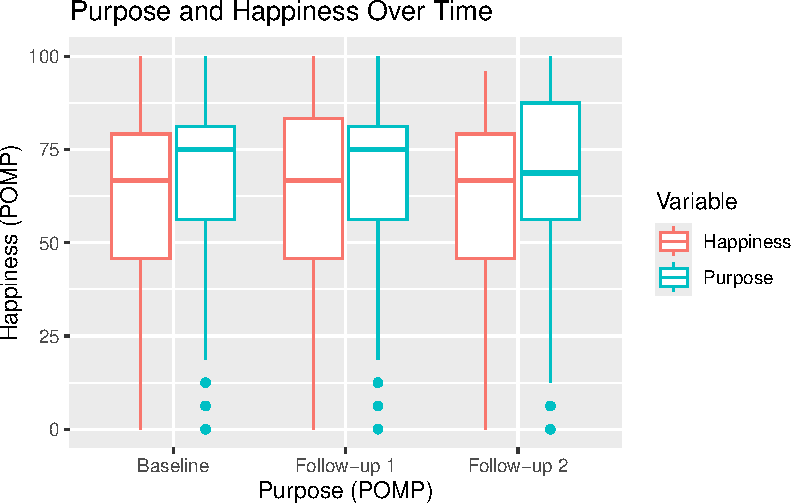
\includegraphics{purpose_vs_happiness_supplement_files/figure-pdf/data_details-1.pdf}

\section{A Comparison of Stability: Purpose
vs.~Happiness}\label{a-comparison-of-stability-purpose-vs.-happiness}

\subsection{Measurement Invariance}\label{measurement-invariance}

\subsubsection{Purpose}\label{purpose}

\subsubsection{Happiness}\label{happiness}

\subsection{Specificity Tests}\label{specificity-tests}

\subsection{Happiness}\label{happiness-1}

\begin{Shaded}
\begin{Highlighting}[]
\CommentTok{\# Happiness}
\NormalTok{datPvH\_shs\_bpurp }\SpecialCharTok{\%\textgreater{}\%} 
  \FunctionTok{select}\NormalTok{(b\_shs\_mean\_POMP, fu1\_shs\_mean\_POMP, fu2\_shs\_mean\_POMP) }\SpecialCharTok{\%\textgreater{}\%}
  \FunctionTok{rename}\NormalTok{(}\AttributeTok{Baseline =}\NormalTok{ b\_shs\_mean\_POMP,}
         \AttributeTok{FollowUp1 =}\NormalTok{ fu1\_shs\_mean\_POMP,}
         \AttributeTok{FollowUp2 =}\NormalTok{ fu2\_shs\_mean\_POMP) }\SpecialCharTok{\%\textgreater{}\%}
  \FunctionTok{pairs.panels}\NormalTok{()}
\end{Highlighting}
\end{Shaded}

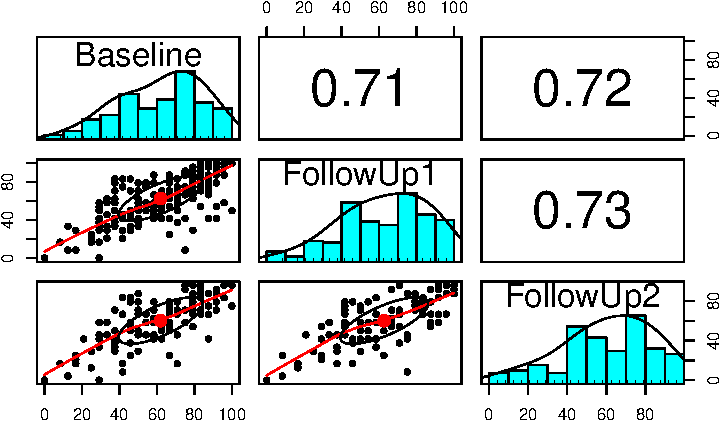
\includegraphics{purpose_vs_happiness_supplement_files/figure-pdf/purpose-1.pdf}

\begin{Shaded}
\begin{Highlighting}[]
\CommentTok{\# Purpose}
\NormalTok{datPvH\_shs\_bpurp }\SpecialCharTok{\%\textgreater{}\%}
  \FunctionTok{select}\NormalTok{(b\_bpurp\_mean\_POMP, fu1\_bpurp\_mean\_POMP, fu2\_bpurp\_mean\_POMP) }\SpecialCharTok{\%\textgreater{}\%}
  \FunctionTok{rename}\NormalTok{(}\AttributeTok{Baseline =}\NormalTok{ b\_bpurp\_mean\_POMP,}
         \AttributeTok{FollowUp1 =}\NormalTok{ fu1\_bpurp\_mean\_POMP,}
         \AttributeTok{FollowUp2 =}\NormalTok{ fu2\_bpurp\_mean\_POMP) }\SpecialCharTok{\%\textgreater{}\%}
  \FunctionTok{pairs.panels}\NormalTok{()}
\end{Highlighting}
\end{Shaded}

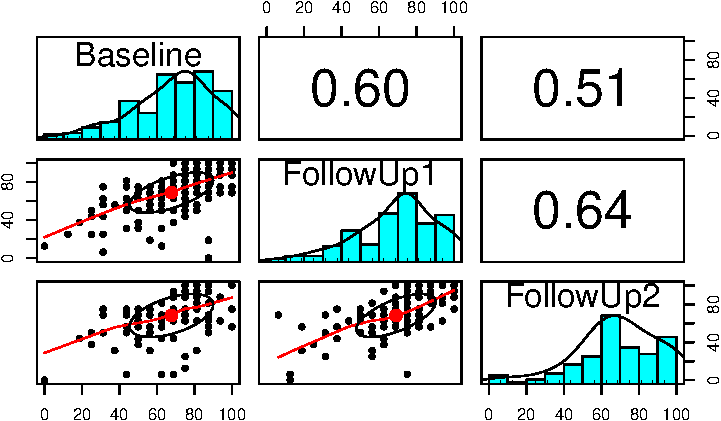
\includegraphics{purpose_vs_happiness_supplement_files/figure-pdf/purpose-2.pdf}

\section{Longitudinal Changes in Purpose and
Happiness}\label{longitudinal-changes-in-purpose-and-happiness}

\begin{Shaded}
\begin{Highlighting}[]
\CommentTok{\# select all bpurp and shs variables in the dataset}

\CommentTok{\# plot the longitudinal changes in purpose and happiness}
\NormalTok{datPvH\_shs\_bpurp\_long }\SpecialCharTok{\%\textgreater{}\%} 
  \FunctionTok{ggplot}\NormalTok{(}\FunctionTok{aes}\NormalTok{(}\AttributeTok{x =}\NormalTok{ time, }\AttributeTok{y =} \StringTok{\textasciigrave{}}\AttributeTok{POMP Score}\StringTok{\textasciigrave{}}\NormalTok{, }\AttributeTok{color =}\NormalTok{ Variable)) }\SpecialCharTok{+}
  \FunctionTok{geom\_boxplot}\NormalTok{() }\SpecialCharTok{+}
  \FunctionTok{labs}\NormalTok{(}\AttributeTok{title =} \StringTok{"Longitudinal Changes in Purpose and Happiness"}\NormalTok{,}
       \AttributeTok{x =} \StringTok{"Time"}\NormalTok{,}
       \AttributeTok{y =} \StringTok{"POMP Score"}\NormalTok{)}
\end{Highlighting}
\end{Shaded}

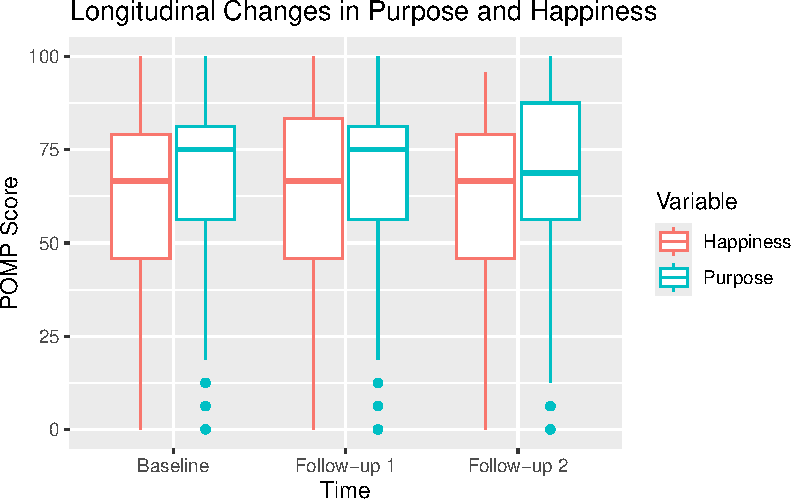
\includegraphics{purpose_vs_happiness_supplement_files/figure-pdf/longitudinal_changes-1.pdf}

\begin{Shaded}
\begin{Highlighting}[]
\NormalTok{datPvH\_shs\_bpurp\_long}\SpecialCharTok{$}\NormalTok{months }\OtherTok{\textless{}{-}} \FunctionTok{case\_match}\NormalTok{(datPvH\_shs\_bpurp\_long}\SpecialCharTok{$}\NormalTok{time,}
                                           \StringTok{"Baseline"} \SpecialCharTok{\textasciitilde{}} \DecValTok{0}\NormalTok{,}
                                           \StringTok{"Follow{-}up 1"} \SpecialCharTok{\textasciitilde{}} \DecValTok{6}\NormalTok{,}
                                           \StringTok{"Follow{-}up 2"} \SpecialCharTok{\textasciitilde{}} \DecValTok{24}\NormalTok{)}
\CommentTok{\# plot the longitudinal data }
\end{Highlighting}
\end{Shaded}

\section{How about self vs.~informant
reports?}\label{how-about-self-vs.-informant-reports}

\subsection{Is Happiness Obvious?}\label{is-happiness-obvious}

\begin{Shaded}
\begin{Highlighting}[]
\CommentTok{\# select only the necessary variables}
\NormalTok{datPvH\_self\_informant }\OtherTok{\textless{}{-}}\NormalTok{ datPvH }\SpecialCharTok{\%\textgreater{}\%} 
  \FunctionTok{select}\NormalTok{(id, b\_shs\_mean\_POMP, INF\_SHS\_mean\_POMP) }\SpecialCharTok{\%\textgreater{}\%}
  \FunctionTok{rename}\NormalTok{(}\AttributeTok{Happiness =}\NormalTok{ b\_shs\_mean\_POMP,}
         \AttributeTok{Happiness\_INF =}\NormalTok{ INF\_SHS\_mean\_POMP)}


\CommentTok{\# plot the self vs. informant reports}
\NormalTok{datPvH\_self\_informant }\SpecialCharTok{\%\textgreater{}\%} 
  \FunctionTok{ggplot}\NormalTok{(}\FunctionTok{aes}\NormalTok{(}\AttributeTok{x =}\NormalTok{ Happiness, }\AttributeTok{y =}\NormalTok{ Happiness\_INF)) }\SpecialCharTok{+}
  \FunctionTok{geom\_point}\NormalTok{() }\SpecialCharTok{+}
  \FunctionTok{geom\_smooth}\NormalTok{(}\AttributeTok{method =} \StringTok{"lm"}\NormalTok{) }\SpecialCharTok{+}
  \FunctionTok{labs}\NormalTok{(}\AttributeTok{title =} \StringTok{"Self vs. Informant Reports of Happiness"}\NormalTok{,}
       \AttributeTok{x =} \StringTok{"Self"}\NormalTok{,}
       \AttributeTok{y =} \StringTok{"Informant"}\NormalTok{) }\SpecialCharTok{+}
  \FunctionTok{geom\_abline}\NormalTok{(}\AttributeTok{intercept =} \DecValTok{0}\NormalTok{, }\AttributeTok{slope =} \DecValTok{1}\NormalTok{, }\AttributeTok{color =} \StringTok{"red"}\NormalTok{) }\SpecialCharTok{+}
  \FunctionTok{xlim}\NormalTok{(}\DecValTok{0}\NormalTok{, }\DecValTok{100}\NormalTok{) }\SpecialCharTok{+}
  \FunctionTok{ylim}\NormalTok{(}\DecValTok{0}\NormalTok{, }\DecValTok{100}\NormalTok{)}
\end{Highlighting}
\end{Shaded}

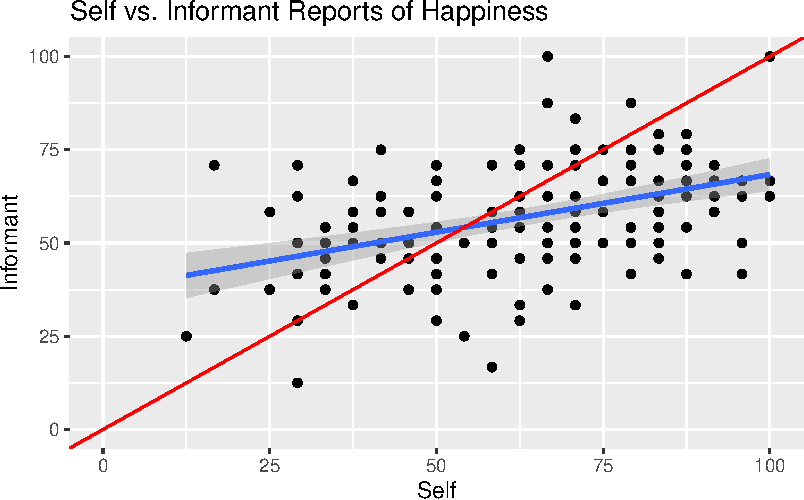
\includegraphics{purpose_vs_happiness_supplement_files/figure-pdf/self_vs_informant-1.pdf}

\section{DATA SUMMARY}\label{data-summary}

\subsection{Variable Names and Labels}\label{variable-names-and-labels}

\begin{Shaded}
\begin{Highlighting}[]
\CommentTok{\# Exctract the varnames and labels from the spss sav file and format for display in the quarto doc}

\CommentTok{\#kable(getQuests(datPvH), col.names = c("Variable", "Label"))}
\CommentTok{\#kable(gQs(datPvH))\#, col.names = c("Column", "Variable", "Label"))}

\FunctionTok{gQs2}\NormalTok{(datPvH)}
\end{Highlighting}
\end{Shaded}

\begin{longtable}[t]{>{}cll}
\toprule
Column & VariableName & Label\\
\midrule
\textbf{1} & id & Please enter the three-digit study ID that you were given in our original email.\\
\textbf{2} & B\_Final\_Results & Baseline - Participant wants to be emailed with the final results (Y or N)\\
\textbf{3} & b\_sdate & Baseline - Timing - First Click\\
\textbf{4} & b\_edate & Baseline - Timing - Last Click\\
\textbf{5} & b\_dur & Baseline - Timing - Page Submit\\
\addlinespace
\textbf{6} & b\_time1\_clicks & Baseline - Timing - Click Count\\
\textbf{7} & Woke & Yesterday, I woke up at\\
\textbf{8} & WokeAMPM & Please choose the correct time period when you woke up\\
\textbf{9} & Bed & Yesterday, I went to bed at\\
\textbf{10} & BedAMPM & Please choose the correct time period when you went to bed\\
\addlinespace
\textbf{11} & Action\_E1\_1 & Activities - Selected Choice Commuting\\
\textbf{12} & Action\_E1\_2 & Activities - Selected Choice Shopping\\
\textbf{13} & Action\_E1\_3 & Activities - Selected Choice Doing housework\\
\textbf{14} & Action\_E1\_4 & Activities - Selected Choice Eating\\
\textbf{15} & Action\_E1\_5 & Activities - Selected Choice Socializing\\
\addlinespace
\textbf{16} & Action\_E1\_6 & Activities - Selected Choice Nap/resting\\
\textbf{17} & Action\_E1\_7 & Activities - Selected Choice Relaxing\\
\textbf{18} & Action\_E1\_8 & Activities - Selected Choice Sex\\
\textbf{19} & Action\_E1\_9 & Activities - Selected Choice Working\\
\textbf{20} & Action\_E1\_10 & Activities - Selected Choice Studying\\
\addlinespace
\textbf{21} & Action\_E1\_11 & Activities - Selected Choice Emailing\\
\textbf{22} & Action\_E1\_12 & Activities - Selected Choice Preparing food\\
\textbf{23} & Action\_E1\_13 & Activities - Selected Choice Taking care of children\\
\textbf{24} & Action\_E1\_14 & Activities - Selected Choice Watching TV\\
\textbf{25} & Action\_E1\_15 & Activities - Selected Choice Leisurely Reading\\
\addlinespace
\textbf{26} & Action\_E1\_16 & Activities - Selected Choice Exercising\\
\textbf{27} & Action\_E1\_17 & Activities - Selected Choice Video/computer games\\
\textbf{28} & Action\_E1\_18 & Activities - Selected Choice Volunteering\\
\textbf{29} & Action\_E1\_19 & Activities - Selected Choice Other:\\
\textbf{30} & Social\_E1\_1 & Social Interactions What - Yes: In-person\\
\addlinespace
\textbf{31} & Social\_E1\_2 & Social Interactions What - Yes: Phone/Skype\\
\textbf{32} & Social\_E1\_3 & Social Interactions What - Yes: Texting/Instant Messaging\\
\textbf{33} & Social\_E1\_4 & Social Interactions What - No: Not interacting with anyone\\
\textbf{34} & Person\_E1\_1 & Social Interactions Who: in-person - Selected Choice Romantic partner/Spouse\\
\textbf{35} & Person\_E1\_2 & Social Interactions Who: in-person - Selected Choice Friend\\
\addlinespace
\textbf{36} & Person\_E1\_3 & Social Interactions Who: in-person - Selected Choice Classmate\\
\textbf{37} & Person\_E1\_4 & Social Interactions Who: in-person - Selected Choice Acquaintance\\
\textbf{38} & Person\_E1\_5 & Social Interactions Who: in-person - Selected Choice Stranger\\
\textbf{39} & Person\_E1\_6 & Social Interactions Who: in-person - Selected Choice My children\\
\textbf{40} & Person\_E1\_7 & Social Interactions Who: in-person - Selected Choice Parents\\
\addlinespace
\textbf{41} & Person\_E1\_8 & Social Interactions Who: in-person - Selected Choice Other Relatives\\
\textbf{42} & Person\_E1\_9 & Social Interactions Who: in-person - Selected Choice Boss\\
\textbf{43} & Person\_E1\_10 & Social Interactions Who: in-person - Selected Choice Co-worker\\
\textbf{44} & Person\_E1\_11 & Social Interactions Who: in-person - Selected Choice Employee/Supervisee\\
\textbf{45} & Person\_E1\_12 & Social Interactions Who: in-person - Selected Choice Client/Customer\\
\addlinespace
\textbf{46} & Person\_E1\_13 & Social Interactions Who: in-person - Selected Choice Other:\\
\textbf{47} & Phone\_E1\_1 & Social Interaction Who: phone/skype - Selected Choice Romantic partner/Spouse\\
\textbf{48} & Phone\_E1\_2 & Social Interaction Who: phone/skype - Selected Choice Friend\\
\textbf{49} & Phone\_E1\_3 & Social Interaction Who: phone/skype - Selected Choice Classmate\\
\textbf{50} & Phone\_E1\_4 & Social Interaction Who: phone/skype - Selected Choice Acquaintance\\
\addlinespace
\textbf{51} & Phone\_E1\_5 & Social Interaction Who: phone/skype - Selected Choice Stranger\\
\textbf{52} & Phone\_E1\_6 & Social Interaction Who: phone/skype - Selected Choice My children\\
\textbf{53} & Phone\_E1\_7 & Social Interaction Who: phone/skype - Selected Choice Parents\\
\textbf{54} & Phone\_E1\_8 & Social Interaction Who: phone/skype - Selected Choice Other Relatives\\
\textbf{55} & Phone\_E1\_9 & Social Interaction Who: phone/skype - Selected Choice Boss\\
\addlinespace
\textbf{56} & Phone\_E1\_10 & Social Interaction Who: phone/skype - Selected Choice Co-worker\\
\textbf{57} & Phone\_E1\_11 & Social Interaction Who: phone/skype - Selected Choice Employee/Supervisee\\
\textbf{58} & Phone\_E1\_12 & Social Interaction Who: phone/skype - Selected Choice Client/Customer\\
\textbf{59} & Phone\_E1\_13 & Social Interaction Who: phone/skype - Selected Choice Other:\\
\textbf{60} & Text\_E1\_1 & Social Interaction Who: text/instant messenger - Selected Choice Romantic partner/Spouse\\
\addlinespace
\textbf{61} & Text\_E1\_2 & Social Interaction Who: text/instant messenger - Selected Choice Friend\\
\textbf{62} & Text\_E1\_3 & Social Interaction Who: text/instant messenger - Selected Choice Classmate\\
\textbf{63} & Text\_E1\_4 & Social Interaction Who: text/instant messenger - Selected Choice Acquaintance\\
\textbf{64} & Text\_E1\_5 & Social Interaction Who: text/instant messenger - Selected Choice Stranger\\
\textbf{65} & Text\_E1\_6 & Social Interaction Who: text/instant messenger - Selected Choice My children\\
\addlinespace
\textbf{66} & Text\_E1\_7 & Social Interaction Who: text/instant messenger - Selected Choice Parents\\
\textbf{67} & Text\_E1\_8 & Social Interaction Who: text/instant messenger - Selected Choice Other Relatives\\
\textbf{68} & Text\_E1\_9 & Social Interaction Who: text/instant messenger - Selected Choice Boss\\
\textbf{69} & Text\_E1\_10 & Social Interaction Who: text/instant messenger - Selected Choice Co-worker\\
\textbf{70} & Text\_E1\_11 & Social Interaction Who: text/instant messenger - Selected Choice Employee/Supervisee\\
\addlinespace
\textbf{71} & Text\_E1\_12 & Social Interaction Who: text/instant messenger - Selected Choice Client/Customer\\
\textbf{72} & Text\_E1\_13 & Social Interaction Who: text/instant messenger - Selected Choice Other:\\
\textbf{73} & ERank\_1 & All Episode Impact - [QID5-ChoiceTextEntryValue]\\
\textbf{74} & ERank\_2 & All Episode Impact - [QID275-ChoiceTextEntryValue]\\
\textbf{75} & ERank\_3 & All Episode Impact - [QID298-ChoiceTextEntryValue]\\
\addlinespace
\textbf{76} & ERank\_4 & All Episode Impact - [QID321-ChoiceTextEntryValue]\\
\textbf{77} & ERank\_5 & All Episode Impact - [QID344-ChoiceTextEntryValue]\\
\textbf{78} & b\_pf1\_o\_1 & Baseline - Psychological Flexibility - items for first goal - This goal is central to my life.\\
\textbf{79} & b\_pf1\_o\_2 & Baseline - Psychological Flexibility - items for first goal - I find this goal challenging.\\
\textbf{80} & b\_pf1\_o\_3 & Baseline - Psychological Flexibility - items for first goal - I feel stressed pursuing this goal.\\
\addlinespace
\textbf{81} & b\_pf1\_o\_4 & Baseline - Psychological Flexibility - items for first goal - I experience negative emotions while pursuing this goal (such as anxiety, frustration, guilt, anger, disappointment).\\
\textbf{82} & b\_pf1\_av\_5\_nr & Baseline - Psychological Flexibility - items for first goal - I avoid the most difficult goal-related tasks.\\
\textbf{83} & b\_pf1\_av\_6\_nr & Baseline - Psychological Flexibility - items for first goal - I put off uncomfortable tasks related to this goal for as long as possible.\\
\textbf{84} & b\_pf1\_av\_7\_nr & Baseline - Psychological Flexibility - items for first goal - I put off pursuing this goal when I could be doing a more enjoyable task.\\
\textbf{85} & b\_pf1\_av\_8\_nr & Baseline - Psychological Flexibility - items for first goal - When I feel stressed pursuing this goal, I give up.\\
\addlinespace
\textbf{86} & b\_pf1\_av\_9\_nr & Baseline - Psychological Flexibility - items for first goal - I get so caught up in thoughts and feelings that I am unable to pursue this goal.\\
\textbf{87} & b\_pf1\_av\_10\_nr & Baseline - Psychological Flexibility - items for first goal - When I feel discouraged, I let my commitment for this goal slide.\\
\textbf{88} & b\_pf1\_av5\_mean\_nr & Baseline - Psychological Flexibility - Average of non-reverse-scored Avoidance items\\
\textbf{89} & b\_pf1\_av5\_mean\_nr\_POMP & B\_PF1\_Av5\_mean\_NR / 6 * 100\\
\textbf{90} & b\_pf1\_ac\_11 & Baseline - Psychological Flexibility - items for first goal - I remain calm when upsetting thoughts arise while pursuing this goal.\\
\addlinespace
\textbf{91} & b\_pf1\_ac\_12 & Baseline - Psychological Flexibility - items for first goal - I accept the setbacks while pursuing this goal.\\
\textbf{92} & b\_pf1\_ac\_13 & Baseline - Psychological Flexibility - items for first goal - While pursuing this goal, I try to accept my negative thoughts and feelings rather than resist them.\\
\textbf{93} & b\_pf1\_ac\_14 & Baseline - Psychological Flexibility - items for first goal - I am willing to experience negative thoughts and emotions related to this goal.\\
\textbf{94} & b\_pf1\_ac\_15 & Baseline - Psychological Flexibility - items for first goal - I accept things I cannot change about this goal.\\
\textbf{95} & b\_pf1\_ac\_16 & Baseline - Psychological Flexibility - items for first goal - While pursuing this goal, I can observe unpleasant feelings without being drawn into them.\\
\addlinespace
\textbf{96} & b\_pf1\_h\_17 & Baseline - Psychological Flexibility - items for first goal - Considering what can go wrong when pursuing this goal helps me prepare for it.\\
\textbf{97} & b\_pf1\_h\_18 & Baseline - Psychological Flexibility - items for first goal - When faced with obstacles related to this goal, my frustration serves to energize me.\\
\textbf{98} & b\_pf1\_h\_19 & Baseline - Psychological Flexibility - items for first goal - I find worrying helpful to solving goal-related problems.\\
\textbf{99} & b\_pf1\_h\_20 & Baseline - Psychological Flexibility - items for first goal - When people distract me from this goal, I use any anger that arises to stay focused.\\
\textbf{100} & b\_pf1\_h\_21 & Baseline - Psychological Flexibility - items for first goal - When I fail to meet my own expectations pursuing this goal, my guilt motivates me.\\
\addlinespace
\textbf{101} & b\_pf1\_h\_22 & Baseline - Psychological Flexibility - items for first goal - I find unpleasant emotions useful for reaching this goal.\\
\textbf{102} & b\_pf1\_val & Baseline - Psychological Flexibility - value first goal\\
\textbf{103} & b\_pf2\_goal & Baseline - Psychological Flexibility - second goal itself\\
\textbf{104} & b\_pf2\_o\_1 & Baseline - Psychological Flexibility - Items for second goal - This goal is central to my life.\\
\textbf{105} & b\_pf2\_o\_2 & Baseline - Psychological Flexibility - Items for second goal - I find this goal challenging.\\
\addlinespace
\textbf{106} & b\_pf2\_o\_3 & Baseline - Psychological Flexibility - Items for second goal - I feel stressed pursuing this goal.\\
\textbf{107} & b\_pf2\_o\_4 & Baseline - Psychological Flexibility - Items for second goal - I experience negative emotions while pursuing this goal (such as anxiety, frustration, guilt, anger, disappointment).\\
\textbf{108} & b\_pf2\_av\_5\_nr & Baseline - Psychological Flexibility - Items for second goal - I avoid the most difficult goal-related tasks.\\
\textbf{109} & b\_pf2\_av\_6\_nr & Baseline - Psychological Flexibility - Items for second goal - I put off uncomfortable tasks related to this goal for as long as possible.\\
\textbf{110} & b\_pf2\_av\_7\_nr & Baseline - Psychological Flexibility - Items for second goal - I put off pursuing this goal when I could be doing a more enjoyable task.\\
\addlinespace
\textbf{111} & b\_pf2\_av\_8\_nr & Baseline - Psychological Flexibility - Items for second goal - When I feel stressed pursuing this goal, I give up.\\
\textbf{112} & b\_pf2\_av\_9\_nr & Baseline - Psychological Flexibility - Items for second goal - I get so caught up in thoughts and feelings that I am unable to pursue this goal.\\
\textbf{113} & b\_pf2\_av\_10\_nr & Baseline - Psychological Flexibility - Items for second goal - When I feel discouraged, I let my commitment for this goal slide.\\
\textbf{114} & b\_pf2\_ac\_11 & Baseline - Psychological Flexibility - Items for second goal - I remain calm when upsetting thoughts arise while pursuing this goal.\\
\textbf{115} & b\_pf2\_ac\_12 & Baseline - Psychological Flexibility - Items for second goal - I accept the setbacks while pursuing this goal.\\
\addlinespace
\textbf{116} & b\_pf2\_ac\_13 & Baseline - Psychological Flexibility - Items for second goal - While pursuing this goal, I try to accept my negative thoughts and feelings rather than resist them.\\
\textbf{117} & b\_pf2\_ac\_14 & Baseline - Psychological Flexibility - Items for second goal - I am willing to experience negative thoughts and emotions related to this goal.\\
\textbf{118} & b\_pf2\_ac\_15 & Baseline - Psychological Flexibility - Items for second goal - I accept things I cannot change about this goal.\\
\textbf{119} & b\_pf2\_ac\_16 & Baseline - Psychological Flexibility - Items for second goal - While pursuing this goal, I can observe unpleasant feelings without being drawn into them.\\
\textbf{120} & b\_pf2\_h\_17 & Baseline - Psychological Flexibility - Items for second goal - Considering what can go wrong when pursuing this goal helps me prepare for it.\\
\addlinespace
\textbf{121} & b\_pf2\_h\_18 & Baseline - Psychological Flexibility - Items for second goal - When faced with obstacles related to this goal, my frustration serves to energize me.\\
\textbf{122} & b\_pf2\_h\_19 & Baseline - Psychological Flexibility - Items for second goal - I find worrying helpful to solving goal-related problems.\\
\textbf{123} & b\_pf2\_h\_20 & Baseline - Psychological Flexibility - Items for second goal - When people distract me from this goal, I use any anger that arises to stay focused.\\
\textbf{124} & b\_pf2\_h\_21 & Baseline - Psychological Flexibility - Items for second goal - When I fail to meet my own expectations pursuing this goal, my guilt motivates me.\\
\textbf{125} & b\_pf2\_h\_22 & Baseline - Psychological Flexibility - Items for second goal - I find unpleasant emotions useful for reaching this goal.\\
\addlinespace
\textbf{126} & b\_pf2\_val & Baseline - Psychological Flexibility - values second goal\\
\textbf{127} & b\_pf\_av\_5\_R\_goals1\_2 & Baseline - Combined PF - av5 - Reverse Coded (averaged av5 score for goals 1 and 2)\\
\textbf{128} & b\_pf\_av\_6\_R\_goals1\_2 & Baseline - Combined PF - av6 - Reverse Coded (averaged av6 score for goals 1 and 2)\\
\textbf{129} & b\_pf\_av\_7\_R\_goals1\_2 & Baseline - Combined PF - av7 - Reverse Coded (averaged av7 score for goals 1 and 2)\\
\textbf{130} & b\_pf\_av\_8\_R\_goals1\_2 & Baseline - Combined PF - av8 - Reverse Coded (averaged av8 score for goals 1 and 2)\\
\addlinespace
\textbf{131} & b\_pf\_av\_9\_R\_goals1\_2 & Baseline - Combined PF - av9 - Reverse Coded (averaged av9 score for goals 1 and 2)\\
\textbf{132} & b\_pf\_av\_10\_R\_goals1\_2 & Baseline - Combined PF - av10 - Reverse Coded (averaged av10 score for goals 1 and 2)\\
\textbf{133} & b\_pf\_ac\_11\_goals1\_2 & Baseline - Combined PF - ac11 (averaged ac11 score for goals 1 and 2)\\
\textbf{134} & b\_pf\_ac\_12\_goals1\_2 & Baseline - Combined PF - ac12 (averaged ac12 score for goals 1 and 2)\\
\textbf{135} & b\_pf\_ac\_13\_goals1\_2 & Baseline - Combined PF - ac13 (averaged ac13 score for goals 1 and 2)\\
\addlinespace
\textbf{136} & b\_pf\_ac\_14\_goals1\_2 & Baseline - Combined PF - ac14 (averaged ac14 score for goals 1 and 2)\\
\textbf{137} & b\_pf\_ac\_15\_goals1\_2 & Baseline - Combined PF - ac15 (averaged ac15 score for goals 1 and 2)\\
\textbf{138} & b\_pf\_ac\_16\_goals1\_2 & Baseline - Combined PF - ac16 (averaged ac16 score for goals 1 and 2)\\
\textbf{139} & b\_pf\_h\_17\_goals1\_2 & Baseline - Combined PF - h17 (averaged h17 score for goals 1 and 2)\\
\textbf{140} & b\_pf\_h\_18\_goals1\_2 & Baseline - Combined PF - h18 (averaged h18 score for goals 1 and 2)\\
\addlinespace
\textbf{141} & b\_pf\_h\_19\_goals1\_2 & Baseline - Combined PF - h19 (averaged h19 score for goals 1 and 2)\\
\textbf{142} & b\_pf\_h\_20\_goals1\_2 & Baseline - Combined PF - h20 (averaged h20 score for goals 1 and 2)\\
\textbf{143} & b\_pf\_h\_21\_goals1\_2 & Baseline - Combined PF - h21 (averaged h21 score for goals 1 and 2)\\
\textbf{144} & b\_pf\_h\_22\_goals1\_2 & Baseline - Combined PF - h22 (averaged h22 score for goals 1 and 2)\\
\textbf{145} & b\_pf\_av5\_mean\_goals1\_2 & Baseline - Combined PF - Avoidance 5-item subscale (mean of goal 1 and 2 averaged avoidance items)\\
\addlinespace
\textbf{146} & b\_pf\_ac5\_mean\_goals1\_2 & Baseline - Combined PF - Acceptance 5-item subscale (mean of goal 1 and 2 averaged acceptance items)\\
\textbf{147} & b\_pf\_h5\_mean\_goals1\_2 & Baseline - Combined PF - Harnessing 5-item subscale (mean of goal 1 and 2 averaged harnessing items)\\
\textbf{148} & b\_ep\_1 & Baseline - Emotion Prejudice Measure - How much will you pay to EXPERIENCE a situation where you feel JOY?\\
\textbf{149} & b\_ep\_2 & Baseline - Emotion Prejudice Measure - How much will you pay to EXPERIENCE a situation where you feel GRATITUDE?\\
\textbf{150} & b\_ep\_3 & Baseline - Emotion Prejudice Measure - How much will you pay to EXPERIENCE a situation where you feel CONTENTMENT?\\
\addlinespace
\textbf{151} & b\_ep\_4 & Baseline - Emotion Prejudice Measure - How much will you pay to EXPERIENCE a situation when you feel INTEREST?\\
\textbf{152} & b\_ep\_5 & Baseline - Emotion Prejudice Measure - How much will you pay to EXPERIENCE a situation where you feel AWE?\\
\textbf{153} & b\_ep\_6 & Baseline - Emotion Prejudice Measure - How much will you pay to AVOID a situation where you feel ANGER?\\
\textbf{154} & b\_ep\_7 & Baseline - Emotion Prejudice Measure - How much will you pay to AVOID a situation where you feel EMBARRASSMENT?\\
\textbf{155} & b\_ep\_8 & Baseline - Emotion Prejudice Measure - How much will you pay to AVOID a situation where you feel GUILT?\\
\addlinespace
\textbf{156} & b\_ep\_9 & Baseline - Emotion Prejudice Measure - How much will you pay to AVOID a situation where you feel AFRAID?\\
\textbf{157} & b\_ep\_10 & Baseline - Emotion Prejudice Measure - How much will you pay to AVOID a situation where you feel SAD?\\
\textbf{158} & b\_5dc\_je\_1 & Baseline - Multidimensional Curiosity Measure - I view challenging situations as an opportunity to grow and learn.\\
\textbf{159} & b\_5dc\_je\_2 & Baseline - Multidimensional Curiosity Measure - I am always looking for experiences that challenge how I think about myself and the world.\\
\textbf{160} & b\_5dc\_je\_3 & Baseline - Multidimensional Curiosity Measure - I seek out situations where it is likely that I will have to think in depth about something.\\
\addlinespace
\textbf{161} & b\_5dc\_je\_4 & Baseline - Multidimensional Curiosity Measure - I enjoy learning about subjects that are unfamiliar to me.\\
\textbf{162} & b\_5dc\_je\_5 & Baseline - Multidimensional Curiosity Measure - I find it fascinating to learn new information.\\
\textbf{163} & b\_5dc\_ds\_6 & Baseline - Multidimensional Curiosity Measure - Thinking about solutions to difficult conceptual problems can keep me awake at night.\\
\textbf{164} & b\_5dc\_ds\_7 & Baseline - Multidimensional Curiosity Measure - I can spend hours on a single problem because I just can't rest without knowing the answer.\\
\textbf{165} & b\_5dc\_ds\_8 & Baseline - Multidimensional Curiosity Measure - I feel frustrated if I can't figure out the solution to a problem, so I work even harder to solve it.\\
\addlinespace
\textbf{166} & b\_5dc\_ds\_9 & Baseline - Multidimensional Curiosity Measure - I work relentlessly at problems that I feel must be solved.\\
\textbf{167} & b\_5dc\_ds\_10 & Baseline - Multidimensional Curiosity Measure - It frustrates me when I don't have all of the information I need.\\
\textbf{168} & b\_5dc\_st\_11\_nr & Baseline - Multidimensional Curiosity Measure - The smallest doubt can stop me from seeking out new experiences.\\
\textbf{169} & b\_5dc\_st\_12\_nr & Baseline - Multidimensional Curiosity Measure - I cannot handle the stress that comes from entering uncertain situations.\\
\textbf{170} & b\_5dc\_st\_13\_nr & Baseline - Multidimensional Curiosity Measure - I find it hard to explore new places when I lack confidence in my abilities.\\
\addlinespace
\textbf{171} & b\_5dc\_st\_14\_nr & Baseline - Multidimensional Curiosity Measure - I cannot function well if I am unsure whether a new experience is safe.\\
\textbf{172} & b\_5dc\_st\_15\_nr & Baseline - Multidimensional Curiosity Measure - It is difficult to concentrate when there is a possibility that I will be taken by surprise.\\
\textbf{173} & b\_5dc\_sc\_16 & Baseline - Multidimensional Curiosity Measure - I like to learn about the habits of others.\\
\textbf{174} & b\_5dc\_sc\_17 & Baseline - Multidimensional Curiosity Measure - I like finding out why people behave the way they do.\\
\textbf{175} & b\_5dc\_sc\_18 & Baseline - Multidimensional Curiosity Measure - When other people are having a conversation, I like to find out what it's about.\\
\addlinespace
\textbf{176} & b\_5dc\_sc\_19 & Baseline - Multidimensional Curiosity Measure - When around other people, I like listening to their conversations.\\
\textbf{177} & b\_5dc\_sc\_20 & Baseline - Multidimensional Curiosity Measure - When people quarrel, I like to know what's going on.\\
\textbf{178} & b\_5dc\_ts\_21 & Baseline - Multidimensional Curiosity Measure - The anxiety of doing something new makes me feel excited and alive.\\
\textbf{179} & b\_5dc\_ts\_22 & Baseline - Multidimensional Curiosity Measure - Risk-taking is exciting to me.\\
\textbf{180} & b\_5dc\_ts\_23 & Baseline - Multidimensional Curiosity Measure - When I have free time, I want to do things that are a little scary.\\
\addlinespace
\textbf{181} & b\_5dc\_ts\_24 & Baseline - Multidimensional Curiosity Measure - Creating an adventure as I go is much more appealing than a planned adventure.\\
\textbf{182} & b\_5dc\_ts\_25 & Baseline - Multidimensional Curiosity Measure - I prefer friends who are excitingly unpredictable.\\
\textbf{183} & b\_5dc\_je\_mean & Baseline - 5DC - Joyous Exploration subscale total (mean)\\
\textbf{184} & b\_5dc\_ds\_mean & Baseline - 5DC - Deprivation Sensitivity subscale total (mean)\\
\textbf{185} & b\_5dc\_st\_11\_r & Baseline - Stress Tolerance\_11\_Reverse Coded\\
\addlinespace
\textbf{186} & b\_5dc\_st\_12\_r & Baseline - Stress Tolerance\_12\_Reverse Coded\\
\textbf{187} & b\_5dc\_st\_13\_r & Baseline - Stress Tolerance\_13\_Reverse Coded\\
\textbf{188} & b\_5dc\_st\_14\_r & Baseline - Stress Tolerance\_14\_Reverse Coded\\
\textbf{189} & b\_5dc\_st\_15\_r & Baseline - Stress Tolerance\_15\_Reverse Coded\\
\textbf{190} & b\_5dc\_st\_mean & Baseline - 5DC - Stress Tolerance subscale total (mean)\\
\addlinespace
\textbf{191} & b\_5dc\_sc\_mean & Baseline - 5DC - Social Curiosity subscale total (mean)\\
\textbf{192} & b\_5dc\_ts\_mean & Baseline - 5DC - Thrill Seeking subscale total (mean)\\
\textbf{193} & B\_BFI\_1\_NR & Baseline - Short Big Five - Tends to be quiet. E\\
\textbf{194} & B\_BFI\_2 & Baseline - Short Big Five - Is compassionate, has a soft heart. A\\
\textbf{195} & B\_BFI\_3\_NR & Baseline - Short Big Five - Tends to be disorganized. C\\
\addlinespace
\textbf{196} & B\_BFI\_4 & Baseline - Short Big Five - Worries a lot. N\\
\textbf{197} & B\_BFI\_5 & Baseline - Short Big Five - Is fascinated by art, music, or literature.\\
\textbf{198} & B\_BFI\_6 & Baseline - Short Big Five - Is dominant, acts as a leader. E\\
\textbf{199} & B\_BFI\_7\_NR & Baseline - Short Big Five - Is sometimes rude to others. A\\
\textbf{200} & B\_BFI\_8\_NR & Baseline - Short Big Five - Has difficulty getting started on tasks. C\\
\addlinespace
\textbf{201} & B\_BFI\_9 & Baseline - Short Big Five - Tends to feel depressed, blue. N\\
\textbf{202} & B\_BFI\_10\_NR & Baseline - Short Big Five - Has little interest in abstract ideas.\\
\textbf{203} & B\_BFI\_11 & Baseline - Short Big Five - Is full of energy. E\\
\textbf{204} & B\_BFI\_12 & Baseline - Short Big Five - Assumes the best about people. A\\
\textbf{205} & B\_BFI\_13 & Baseline - Short Big Five - Is reliable, can always be counted on. C\\
\addlinespace
\textbf{206} & B\_BFI\_14\_NR & Baseline - Short Big Five - Is emotionally stable, not easily upset. N\\
\textbf{207} & B\_BFI\_15 & Baseline - Short Big Five - Is original, comes up with new ideas.\\
\textbf{208} & B\_BFI\_16 & Baseline - Short Big Five - Is outgoing, sociable. E\\
\textbf{209} & B\_BFI\_17\_NR & Baseline - Short Big Five - Can be cold and uncaring. A\\
\textbf{210} & B\_BFI\_18 & Baseline - Short Big Five - Keeps things neat and tidy. C\\
\addlinespace
\textbf{211} & B\_BFI\_19\_NR & Baseline - Short Big Five - Is relaxed, handles stress well. N\\
\textbf{212} & B\_BFI\_20\_NR & Baseline - Short Big Five - Has few artistic interests.\\
\textbf{213} & B\_BFI\_21\_NR & Baseline - Short Big Five - Prefers to have others take charge. E\\
\textbf{214} & B\_BFI\_22 & Baseline - Short Big Five - Is respectful, treats others with respect. A\\
\textbf{215} & B\_BFI\_23 & Baseline - Short Big Five - Is persistent, works until the task is finished. C\\
\addlinespace
\textbf{216} & B\_BFI\_24\_NR & Baseline - Short Big Five - Feels secure, comfortable with self. N\\
\textbf{217} & B\_BFI\_25 & Baseline - Short Big Five - Is complex, a deep thinker.\\
\textbf{218} & B\_BFI\_26\_NR & Baseline - Short Big Five - Is less active than other people. E\\
\textbf{219} & B\_BFI\_27\_NR & Baseline - Short Big Five - Tends to find fault with others. A\\
\textbf{220} & B\_BFI\_28\_NR & Baseline - Short Big Five - Can be somewhat careless. C\\
\addlinespace
\textbf{221} & B\_BFI\_29 & Baseline - Short Big Five - Is temperamental, gets emotional easily. N\\
\textbf{222} & B\_BFI\_30\_NR & Baseline - Short Big Five - Has little creativity.\\
\textbf{223} & b\_bmis\_pa\_1 & Baseline - Brief Mood Inspection Scale - Month - Lively\\
\textbf{224} & b\_bmis\_pa\_2 & Baseline - Brief Mood Inspection Scale - Month - Happy\\
\textbf{225} & b\_bmis\_na\_3\_nr & Baseline - Brief Mood Inspection Scale - Month - Sad\\
\addlinespace
\textbf{226} & b\_bmis\_na\_4\_nr & Baseline - Brief Mood Inspection Scale - Month - Tired\\
\textbf{227} & b\_bmis\_pa\_5 & Baseline - Brief Mood Inspection Scale - Month - Caring\\
\textbf{228} & b\_bmis\_pa\_6 & Baseline - Brief Mood Inspection Scale - Month - Content\\
\textbf{229} & b\_bmis\_na\_7\_nr & Baseline - Brief Mood Inspection Scale - Month - Gloomy\\
\textbf{230} & b\_bmis\_na\_8\_nr & Baseline - Brief Mood Inspection Scale - Month - Jittery\\
\addlinespace
\textbf{231} & b\_bmis\_na\_9\_nr & Baseline - Brief Mood Inspection Scale - Month - Drowsy\\
\textbf{232} & b\_bmis\_na\_10\_nr & Baseline - Brief Mood Inspection Scale - Month - Grouchy\\
\textbf{233} & b\_bmis\_pa\_11 & Baseline - Brief Mood Inspection Scale - Month - Peppy\\
\textbf{234} & b\_bmis\_na\_12\_nr & Baseline - Brief Mood Inspection Scale - Month - Nervous\\
\textbf{235} & b\_bmis\_pa\_13\_nr & Baseline - Brief Mood Inspection Scale - Month - Calm\\
\addlinespace
\textbf{236} & b\_bmis\_pa\_14 & Baseline - Brief Mood Inspection Scale - Month - Loving\\
\textbf{237} & b\_bmis\_na\_15\_nr & Baseline - Brief Mood Inspection Scale - Month - Fed Up\\
\textbf{238} & b\_bmis\_pa\_16 & Baseline - Brief Mood Inspection Scale - Month - Active\\
\textbf{239} & b\_bmis\_pm\_17 & Baseline - Brief Mood Inspection Scale - Present - Overall My PRESENT Mood is\\
\textbf{240} & b\_CLRa & Baseline - Attention Check - Color A\\
\addlinespace
\textbf{241} & b\_shs\_gh\_a & Baseline - Subjective Happiness Scale - General Happiness - In general, I consider myself:\\
\textbf{242} & b\_shs\_rh\_a & Baseline - Subjective Happiness Scale - Relative Happiness - Compared to most of my peers, I consider myself:\\
\textbf{243} & b\_shs\_ch\_a & Baseline - Subjective Happiness Scale - Characterization of Happiness - Some people are generally very happy. They enjoy life regardless of what is going on, and get the most out of everything. To what extent does this characterization describe you?\\
\textbf{244} & b\_shs\_ch\_b\_nr & Baseline - Subjective Happiness Scale - Characterization of Happiness - Some people are generally not very happy. Although they are not depressed, they never seem as happy as they might be. To what extend does this characterization describe you?\\
\textbf{245} & b\_shs\_ch\_b\_r & B\_SHS\_4\_reverse scored\\
\addlinespace
\textbf{246} & b\_bmpns\_rs\_1 & Baseline - Balanced Measure of Psychological Needs Scale - I felt a sense of contact with people who care for me, and whom I care for.\\
\textbf{247} & b\_bmpns\_cs\_2 & Baseline - Balanced Measure of Psychological Needs Scale - I was successfully completing difficult tasks and projects.\\
\textbf{248} & b\_bmpns\_as\_3 & Baseline - Balanced Measure of Psychological Needs Scale - I was free to do things my own way.\\
\textbf{249} & b\_bmpns\_rd\_4\_nr & Baseline - Balanced Measure of Psychological Needs Scale - I was lonely.\\
\textbf{250} & b\_bmpns\_cd\_5\_nr & Baseline - Balanced Measure of Psychological Needs Scale - I experienced some kind of failure, or was unable to do well at something.\\
\addlinespace
\textbf{251} & b\_bmpns\_ad\_6\_nr & Baseline - Balanced Measure of Psychological Needs Scale - I had a lot of pressures I could do without.\\
\textbf{252} & b\_bmpns\_rs\_7 & Baseline - Balanced Measure of Psychological Needs Scale - I felt close and connected with other people who are important to me.\\
\textbf{253} & b\_bmpns\_cs\_8 & Baseline - Balanced Measure of Psychological Needs Scale - I took on and mastered hard challenges.\\
\textbf{254} & b\_bmpns\_as\_9 & Baseline - Balanced Measure of Psychological Needs Scale - My choices expressed my ‘‘true self.’’\\
\textbf{255} & b\_bmpns\_rd\_10\_nr & Baseline - Balanced Measure of Psychological Needs Scale - I felt unappreciated by one or more important people.\\
\addlinespace
\textbf{256} & b\_bmpns\_cd\_11\_nr & Baseline - Balanced Measure of Psychological Needs Scale - I did something stupid that made me feel incompetent.\\
\textbf{257} & b\_bmpns\_ad\_12\_nr & Baseline - Balanced Measure of Psychological Needs Scale - There were people telling me what I had to do.\\
\textbf{258} & b\_bmpns\_rs\_13 & Baseline - Balanced Measure of Psychological Needs Scale - I felt a strong sense of intimacy with the people I spent time with.\\
\textbf{259} & b\_bmpns\_cs\_14 & Baseline - Balanced Measure of Psychological Needs Scale - I did well even at the hard things.\\
\textbf{260} & b\_bmpns\_as\_15 & Baseline - Balanced Measure of Psychological Needs Scale - I was really doing what interests me.\\
\addlinespace
\textbf{261} & b\_bmpns\_rd\_16\_nr & Baseline - Balanced Measure of Psychological Needs Scale - I had disagreements or conflicts with people I usually get along with.\\
\textbf{262} & b\_bmpns\_cd\_17\_nr & Baseline - Balanced Measure of Psychological Needs Scale - I struggled doing something I should be good at.\\
\textbf{263} & b\_bmpns\_ad\_18\_nr & Baseline - Balanced Measure of Psychological Needs Scale - I had to do things against my will.\\
\textbf{264} & b\_bmpns\_rd\_4\_r & B\_BMPNS\_rd\_4\_Reverse scored\\
\textbf{265} & b\_bmpns\_cd\_5\_r & B\_BMPNS\_cd\_5\_Reverse scored\\
\addlinespace
\textbf{266} & b\_bmpns\_ad\_6\_r & B\_BMPNS\_ad\_6\_Reverse scored\\
\textbf{267} & b\_bmpns\_rd\_10\_r & B\_BMPNS\_rd\_10\_Reverse scored\\
\textbf{268} & b\_bmpns\_cd\_11\_r & B\_BMPNS\_cd\_11\_Reverse scored\\
\textbf{269} & b\_bmpns\_ad\_12\_r & B\_BMPNS\_ad\_12\_Reverse scored\\
\textbf{270} & b\_bmpns\_rd\_16\_r & B\_BMPNS\_rd\_16\_Reverse scored\\
\addlinespace
\textbf{271} & b\_bmpns\_cd\_17\_r & B\_BMPNS\_cd\_17\_Reverse scored\\
\textbf{272} & b\_bmpns\_ad\_18\_r & B\_BMPNS\_ad\_18\_Reverse scored\\
\textbf{273} & b\_swls\_1 & Baseline - Satisfaction with Life Scale - In most ways my life is close to my ideal.\\
\textbf{274} & b\_swls\_2 & Baseline - Satisfaction with Life Scale - The conditions of my life are excellent.\\
\textbf{275} & b\_swls\_3 & Baseline - Satisfaction with Life Scale - I am satisfied with my life.\\
\addlinespace
\textbf{276} & b\_swls\_4 & Baseline - Satisfaction with Life Scale - So far I have gotten the important things I want in life.\\
\textbf{277} & b\_swls\_5 & Baseline - Satisfaction with Life Scale - If I could live my life over, I would change almost nothing.\\
\textbf{278} & b\_vali\_con\_1 & Baseline - Portrait Values Questionnaire--Importance - I believe I should always show respect to my parents and to older people. It is important to me to be obedient.\\
\textbf{279} & b\_vali\_tra\_2 & Baseline - Portrait Values Questionnaire--Importance - Religious belief is important to me. I try hard to do what my religion requires.\\
\textbf{280} & b\_vali\_ben\_3 & Baseline - Portrait Values Questionnaire--Importance - It's very important to me to help the people around me. I want to care for their well-being.\\
\addlinespace
\textbf{281} & b\_vali\_uni\_4 & Baseline - Portrait Values Questionnaire--Importance - I think it is important that every person in the world be treated equally. I believe everyone should have equal opportunities in life.\\
\textbf{282} & b\_vali\_sd\_5 & Baseline - Portrait Values Questionnaire--Importance - I think it's important to be interested in things. I like to be curious and to try to understand all sorts of things.\\
\textbf{283} & b\_vali\_stim\_6 & Baseline - Portrait Values Questionnaire--Importance - I like to take risks. I am always looking for adventures.\\
\textbf{284} & b\_vali\_hed\_7 & Baseline - Portrait Values Questionnaire--Importance - I seek every chance I can to have fun. It is important to me to do things that give me pleasure.\\
\textbf{285} & b\_vali\_ach\_8 & Baseline - Portrait Values Questionnaire--Importance - Getting ahead in life is important to me. I strive to do better than others.\\
\addlinespace
\textbf{286} & b\_vali\_pow\_9 & Baseline - Portrait Values Questionnaire--Importance - I always want to be the one who makes the decisions. I like to be the leader.\\
\textbf{287} & b\_vali\_sec\_10 & Baseline - Portrait Values Questionnaire--Importance - It is important to me that things be organized and clean. I really do not like things to be a mess.\\
\textbf{288} & b\_vali\_con\_11 & Baseline - Portrait Values Questionnaire--Importance - It is important to me to always behave properly. I want to avoid doing anything people would say is wrong.\\
\textbf{289} & b\_vali\_tra\_12 & Baseline - Portrait Values Questionnaire--Importance - I think it is best to do things in traditional ways. It is important to me to keep up the customs I have learned.\\
\textbf{290} & b\_vali\_ben\_13 & Baseline - Portrait Values Questionnaire--Importance - It is important to me to respond to the needs of others. I try to support those I know.\\
\addlinespace
\textbf{291} & b\_vali\_uni\_14 & Baseline - Portrait Values Questionnaire--Importance - I believe all the worlds' people should live in harmony. Promoting peace among all groups in the world is important to me.\\
\textbf{292} & b\_vali\_sd\_15 & Baseline - Portrait Values Questionnaire--Importance - Thinking up new ideas and being creative is important to me. I like to do things in my own original way.\\
\textbf{293} & b\_vali\_stim\_16 & Baseline - Portrait Values Questionnaire--Importance - I think it is important to do lots of different things in life. I always look for new things to try.\\
\textbf{294} & b\_vali\_hed\_17 & Baseline - Portrait Values Questionnaire--Importance - I really want to enjoy life. Having a good time is very important to me.\\
\textbf{295} & b\_vali\_ach\_18 & Baseline - Portrait Values Questionnaire--Importance - Being very successful is important to me. I like to impress other people.\\
\addlinespace
\textbf{296} & b\_vali\_pow\_19 & Baseline - Portrait Values Questionnaire--Importance - It is important to me to be in charge and tell others what to do. I want people to do what I say.\\
\textbf{297} & b\_vali\_sec\_20 & Baseline - Portrait Values Questionnaire--Importance - Having a stable government is important to me. I am concerned that the social order be protected.\\
\textbf{298} & b\_kdcs\_se\_1\_a & Baseline - Kaufman Domains of Creativity Scale-FREQ - How many times IN THE PAST SIX MONTHS have you done this activity? - Finding something fun to do when I have no money\\
\textbf{299} & b\_kdcs\_se\_2\_a & Baseline - Kaufman Domains of Creativity Scale-FREQ - How many times IN THE PAST SIX MONTHS have you done this activity? - Helping other people cope with a difficult situation\\
\textbf{300} & b\_kdcs\_se\_3\_a & Baseline - Kaufman Domains of Creativity Scale-FREQ - How many times IN THE PAST SIX MONTHS have you done this activity? - Teaching someone how to do something\\
\addlinespace
\textbf{301} & b\_kdcs\_se\_4\_a & Baseline - Kaufman Domains of Creativity Scale-FREQ - How many times IN THE PAST SIX MONTHS have you done this activity? - Maintaining a good balance between my work and personal life\\
\textbf{302} & b\_kdcs\_se\_5\_a & Baseline - Kaufman Domains of Creativity Scale-FREQ - How many times IN THE PAST SIX MONTHS have you done this activity? - Understanding how to make myself happy\\
\textbf{303} & b\_kdcs\_se\_6\_a & Baseline - Kaufman Domains of Creativity Scale-FREQ - How many times IN THE PAST SIX MONTHS have you done this activity? - Being able to work through my personal problems in a healthy way\\
\textbf{304} & b\_kdcs\_se\_7\_a & Baseline - Kaufman Domains of Creativity Scale-FREQ - How many times IN THE PAST SIX MONTHS have you done this activity? - Thinking of new ways to help people\\
\textbf{305} & b\_kdcs\_se\_8\_a & Baseline - Kaufman Domains of Creativity Scale-FREQ - How many times IN THE PAST SIX MONTHS have you done this activity? - Choosing the best solution to a problem\\
\addlinespace
\textbf{306} & b\_kdcs\_se\_9\_a & Baseline - Kaufman Domains of Creativity Scale-FREQ - How many times IN THE PAST SIX MONTHS have you done this activity? - Planning a trip or event with friends that meets everyone's needs\\
\textbf{307} & b\_kdcs\_se\_10\_a & Baseline - Kaufman Domains of Creativity Scale-FREQ - How many times IN THE PAST SIX MONTHS have you done this activity? - Mediating a dispute or argument between two friends\\
\textbf{308} & b\_kdcs\_se\_11\_a & Baseline - Kaufman Domains of Creativity Scale-FREQ - How many times IN THE PAST SIX MONTHS have you done this activity? - Getting people to feel relaxed and at ease\\
\textbf{309} & b\_kdcs\_sc\_12\_a & Baseline - Kaufman Domains of Creativity Scale-FREQ - How many times IN THE PAST SIX MONTHS have you done this activity? - Writing a non-fiction article for a newspaper, newsletter, or magazine\\
\textbf{310} & b\_kdcs\_sc\_13\_a & Baseline - Kaufman Domains of Creativity Scale-FREQ - How many times IN THE PAST SIX MONTHS have you done this activity? - Writing a letter to the editor\\
\addlinespace
\textbf{311} & b\_kdcs\_sc\_14\_a & Baseline - Kaufman Domains of Creativity Scale-FREQ - How many times IN THE PAST SIX MONTHS have you done this activity? - Researching a topic using many different types of sources that may not be readily apparent\\
\textbf{312} & b\_kdcs\_sc\_15\_a & Baseline - Kaufman Domains of Creativity Scale-FREQ - How many times IN THE PAST SIX MONTHS have you done this activity? - Debating a controversial topic from my own perspective\\
\textbf{313} & b\_kdcs\_sc\_16\_a & Baseline - Kaufman Domains of Creativity Scale-FREQ - How many times IN THE PAST SIX MONTHS have you done this activity? - Responding to an issue in a context-appropriate way\\
\textbf{314} & b\_kdcs\_sc\_17\_a & Baseline - Kaufman Domains of Creativity Scale-FREQ - How many times IN THE PAST SIX MONTHS have you done this activity? - Gathering the best possible assortment of articles or papers to support a specific point or view\\
\textbf{315} & b\_kdcs\_sc\_18\_a & Baseline - Kaufman Domains of Creativity Scale-FREQ - How many times IN THE PAST SIX MONTHS have you done this activity? - Arguing a side in a debate that I do not personally agree with\\
\addlinespace
\textbf{316} & b\_kdcs\_sc\_19\_a & Baseline - Kaufman Domains of Creativity Scale-FREQ - How many times IN THE PAST SIX MONTHS have you done this activity? - Analyzing the themes in a good book\\
\textbf{317} & b\_kdcs\_sc\_20\_a & Baseline - Kaufman Domains of Creativity Scale-FREQ - How many times IN THE PAST SIX MONTHS have you done this activity? - Figuring out how to integrate critiques and suggestions while revising a work\\
\textbf{318} & b\_kdcs\_sc\_21\_a & Baseline - Kaufman Domains of Creativity Scale-FREQ - How many times IN THE PAST SIX MONTHS have you done this activity? - Being able to offer constructive feedback based on my own reading of a paper\\
\textbf{319} & b\_kdcs\_sc\_22\_a & Baseline - Kaufman Domains of Creativity Scale-FREQ - How many times IN THE PAST SIX MONTHS have you done this activity? - Coming up with a new way to think about an old debate\\
\textbf{320} & b\_kdcs\_pe\_23\_a & Baseline - Kaufman Domains of Creativity Scale-FREQ - How many times IN THE PAST SIX MONTHS have you done this activity? - Writing a poem\\
\addlinespace
\textbf{321} & b\_kdcs\_pe\_24\_a & Baseline - Kaufman Domains of Creativity Scale-FREQ - How many times IN THE PAST SIX MONTHS have you done this activity? - Making up lyrics to a funny song\\
\textbf{322} & b\_kdcs\_pe\_25\_a & Baseline - Kaufman Domains of Creativity Scale-FREQ - How many times IN THE PAST SIX MONTHS have you done this activity? - Making up rhymes\\
\textbf{323} & b\_kdcs\_pe\_26\_a & Baseline - Kaufman Domains of Creativity Scale-FREQ - How many times IN THE PAST SIX MONTHS have you done this activity? - Composing an original song\\
\textbf{324} & b\_kdcs\_pe\_27\_a & Baseline - Kaufman Domains of Creativity Scale-FREQ - How many times IN THE PAST SIX MONTHS have you done this activity? - Learning how to play a musical instrument\\
\textbf{325} & b\_kdcs\_pe\_28\_a & Baseline - Kaufman Domains of Creativity Scale-FREQ - How many times IN THE PAST SIX MONTHS have you done this activity? - Shooting a fun video to air on YouTube\\
\addlinespace
\textbf{326} & b\_kdcs\_pe\_29\_a & Baseline - Kaufman Domains of Creativity Scale-FREQ - How many times IN THE PAST SIX MONTHS have you done this activity? - Singing in harmony\\
\textbf{327} & b\_kdcs\_pe\_30\_a & Baseline - Kaufman Domains of Creativity Scale-FREQ - How many times IN THE PAST SIX MONTHS have you done this activity? - Spontaneously creating lyrics to a rap song\\
\textbf{328} & b\_kdcs\_pe\_31\_a & Baseline - Kaufman Domains of Creativity Scale-FREQ - How many times IN THE PAST SIX MONTHS have you done this activity? - Playing music in public\\
\textbf{329} & b\_kdcs\_pe\_32\_a & Baseline - Kaufman Domains of Creativity Scale-FREQ - How many times IN THE PAST SIX MONTHS have you done this activity? - Acting in a play\\
\textbf{330} & b\_kdcs\_ms\_33\_a & Baseline - Kaufman Domains of Creativity Scale-FREQ - How many times IN THE PAST SIX MONTHS have you done this activity? - Carving something out of wood or similar material\\
\addlinespace
\textbf{331} & b\_kdcs\_ms\_34\_a & Baseline - Kaufman Domains of Creativity Scale-FREQ - How many times IN THE PAST SIX MONTHS have you done this activity? - Figuring out how to fix a frozen or buggy computer\\
\textbf{332} & b\_kdcs\_ms\_35\_a & Baseline - Kaufman Domains of Creativity Scale-FREQ - How many times IN THE PAST SIX MONTHS have you done this activity? - Writing a computer program\\
\textbf{333} & b\_kdcs\_ms\_36\_a & Baseline - Kaufman Domains of Creativity Scale-FREQ - How many times IN THE PAST SIX MONTHS have you done this activity? - Solving math puzzles\\
\textbf{334} & b\_kdcs\_ms\_37\_a & Baseline - Kaufman Domains of Creativity Scale-FREQ - How many times IN THE PAST SIX MONTHS have you done this activity? - Taking apart machines and figuring out how they work\\
\textbf{335} & b\_kdcs\_ms\_38\_a & Baseline - Kaufman Domains of Creativity Scale-FREQ - How many times IN THE PAST SIX MONTHS have you done this activity? - Building something mechanical (like a robot)\\
\addlinespace
\textbf{336} & b\_kdcs\_ms\_39\_a & Baseline - Kaufman Domains of Creativity Scale-FREQ - How many times IN THE PAST SIX MONTHS have you done this activity? - Helping to carry out or design a scientific experiment\\
\textbf{337} & b\_kdcs\_ms\_40\_a & Baseline - Kaufman Domains of Creativity Scale-FREQ - How many times IN THE PAST SIX MONTHS have you done this activity? - Solving an algebraic or geometric proof\\
\textbf{338} & b\_kdcs\_ms\_41\_a & Baseline - Kaufman Domains of Creativity Scale-FREQ - How many times IN THE PAST SIX MONTHS have you done this activity? - Constructing something out of metal, stone, or similar material\\
\textbf{339} & b\_kdcs\_ac\_42\_a & Baseline - Kaufman Domains of Creativity Scale-FREQ - How many times IN THE PAST SIX MONTHS have you done this activity? - Drawing a picture of something I've never actually seen (like an alien)\\
\textbf{340} & b\_kdcs\_ac\_43\_a & Baseline - Kaufman Domains of Creativity Scale-FREQ - How many times IN THE PAST SIX MONTHS have you done this activity? - Sketching a person or object\\
\addlinespace
\textbf{341} & b\_kdcs\_ac\_44\_a & Baseline - Kaufman Domains of Creativity Scale-FREQ - How many times IN THE PAST SIX MONTHS have you done this activity? - Doodling/Drawing random or geometric designs\\
\textbf{342} & b\_kdcs\_ac\_45\_a & Baseline - Kaufman Domains of Creativity Scale-FREQ - How many times IN THE PAST SIX MONTHS have you done this activity? - Making a scrapbook page out of my photographs\\
\textbf{343} & b\_kdcs\_ac\_46\_a & Baseline - Kaufman Domains of Creativity Scale-FREQ - How many times IN THE PAST SIX MONTHS have you done this activity? - Taking a well-composed photograph using an interesting angle or approach\\
\textbf{344} & b\_kdcs\_ac\_47\_a & Baseline - Kaufman Domains of Creativity Scale-FREQ - How many times IN THE PAST SIX MONTHS have you done this activity? - Making a sculpture or piece of pottery\\
\textbf{345} & b\_kdcs\_ac\_48\_a & Baseline - Kaufman Domains of Creativity Scale-FREQ - How many times IN THE PAST SIX MONTHS have you done this activity? - Appreciating a beautiful painting\\
\addlinespace
\textbf{346} & b\_kdcs\_ac\_49\_a & Baseline - Kaufman Domains of Creativity Scale-FREQ - How many times IN THE PAST SIX MONTHS have you done this activity? - Coming up with my own interpretations of a classic work of art\\
\textbf{347} & b\_kdcs\_ac\_50\_a & Baseline - Kaufman Domains of Creativity Scale-FREQ - How many times IN THE PAST SIX MONTHS have you done this activity? - Enjoying an art museum\\
\textbf{348} & b\_kdcs\_se\_1\_b & Baseline - Kaufman Domains of Creativity Scale-RATING - How creative were you while doing this activity? - Finding something fun to do when I have no money\\
\textbf{349} & b\_kdcs\_se\_2\_b & Baseline - Kaufman Domains of Creativity Scale-RATING - How creative were you while doing this activity? - Helping other people cope with a difficult situation\\
\textbf{350} & b\_kdcs\_se\_3\_b & Baseline - Kaufman Domains of Creativity Scale-RATING - How creative were you while doing this activity? - Teaching someone how to do something\\
\addlinespace
\textbf{351} & b\_kdcs\_se\_4\_b & Baseline - Kaufman Domains of Creativity Scale-RATING - How creative were you while doing this activity? - Maintaining a good balance between my work and personal life\\
\textbf{352} & b\_kdcs\_se\_5\_b & Baseline - Kaufman Domains of Creativity Scale-RATING - How creative were you while doing this activity? - Understanding how to make myself happy\\
\textbf{353} & b\_kdcs\_se\_6\_b & Baseline - Kaufman Domains of Creativity Scale-RATING - How creative were you while doing this activity? - Being able to work through my personal problems in a healthy way\\
\textbf{354} & b\_kdcs\_se\_7\_b & Baseline - Kaufman Domains of Creativity Scale-RATING - How creative were you while doing this activity? - Thinking of new ways to help people\\
\textbf{355} & b\_kdcs\_se\_8\_b & Baseline - Kaufman Domains of Creativity Scale-RATING - How creative were you while doing this activity? - Choosing the best solution to a problem\\
\addlinespace
\textbf{356} & b\_kdcs\_se\_9\_b & Baseline - Kaufman Domains of Creativity Scale-RATING - How creative were you while doing this activity? - Planning a trip or event with friends that meets everyone's needs\\
\textbf{357} & b\_kdcs\_se\_10\_b & Baseline - Kaufman Domains of Creativity Scale-RATING - How creative were you while doing this activity? - Mediating a dispute or argument between two friends\\
\textbf{358} & b\_kdcs\_se\_11\_b & Baseline - Kaufman Domains of Creativity Scale-RATING - How creative were you while doing this activity? - Getting people to feel relaxed and at ease\\
\textbf{359} & b\_kdcs\_sc\_12\_b & Baseline - Kaufman Domains of Creativity Scale-RATING - How creative were you while doing this activity? - Writing a non-fiction article for a newspaper, newsletter, or magazine\\
\textbf{360} & b\_kdcs\_sc\_13\_b & Baseline - Kaufman Domains of Creativity Scale-RATING - How creative were you while doing this activity? - Writing a letter to the editor\\
\addlinespace
\textbf{361} & b\_kdcs\_sc\_14\_b & Baseline - Kaufman Domains of Creativity Scale-RATING - How creative were you while doing this activity? - Researching a topic using many different types of sources that may not be readily apparent\\
\textbf{362} & b\_kdcs\_sc\_15\_b & Baseline - Kaufman Domains of Creativity Scale-RATING - How creative were you while doing this activity? - Debating a controversial topic from my own perspective\\
\textbf{363} & b\_kdcs\_sc\_16\_b & Baseline - Kaufman Domains of Creativity Scale-RATING - How creative were you while doing this activity? - Responding to an issue in a context-appropriate way\\
\textbf{364} & b\_kdcs\_sc\_17\_b & Baseline - Kaufman Domains of Creativity Scale-RATING - How creative were you while doing this activity? - Gathering the best possible assortment of articles or papers to support a specific point or view\\
\textbf{365} & b\_kdcs\_sc\_18\_b & Baseline - Kaufman Domains of Creativity Scale-RATING - How creative were you while doing this activity? - Arguing a side in a debate that I do not personally agree with\\
\addlinespace
\textbf{366} & b\_kdcs\_sc\_19\_b & Baseline - Kaufman Domains of Creativity Scale-RATING - How creative were you while doing this activity? - Analyzing the themes in a good book\\
\textbf{367} & b\_kdcs\_sc\_20\_b & Baseline - Kaufman Domains of Creativity Scale-RATING - How creative were you while doing this activity? - Figuring out how to integrate critiques and suggestions while revising a work\\
\textbf{368} & b\_kdcs\_sc\_21\_b & Baseline - Kaufman Domains of Creativity Scale-RATING - How creative were you while doing this activity? - Being able to offer constructive feedback based on my own reading of a paper\\
\textbf{369} & b\_kdcs\_sc\_22\_b & Baseline - Kaufman Domains of Creativity Scale-RATING - How creative were you while doing this activity? - Coming up with a new way to think about an old debate\\
\textbf{370} & b\_kdcs\_pe\_23\_b & Baseline - Kaufman Domains of Creativity Scale-RATING - How creative were you while doing this activity? - Writing a poem\\
\addlinespace
\textbf{371} & b\_kdcs\_pe\_24\_b & Baseline - Kaufman Domains of Creativity Scale-RATING - How creative were you while doing this activity? - Making up lyrics to a funny song\\
\textbf{372} & b\_kdcs\_pe\_25\_b & Baseline - Kaufman Domains of Creativity Scale-RATING - How creative were you while doing this activity? - Making up rhymes\\
\textbf{373} & b\_kdcs\_pe\_26\_b & Baseline - Kaufman Domains of Creativity Scale-RATING - How creative were you while doing this activity? - Composing an original song\\
\textbf{374} & b\_kdcs\_pe\_27\_b & Baseline - Kaufman Domains of Creativity Scale-RATING - How creative were you while doing this activity? - Learning how to play a musical instrument\\
\textbf{375} & b\_kdcs\_pe\_28\_b & Baseline - Kaufman Domains of Creativity Scale-RATING - How creative were you while doing this activity? - Shooting a fun video to air on YouTube\\
\addlinespace
\textbf{376} & b\_kdcs\_pe\_29\_b & Baseline - Kaufman Domains of Creativity Scale-RATING - How creative were you while doing this activity? - Singing in harmony\\
\textbf{377} & b\_kdcs\_pe\_30\_b & Baseline - Kaufman Domains of Creativity Scale-RATING - How creative were you while doing this activity? - Spontaneously creating lyrics to a rap song\\
\textbf{378} & b\_kdcs\_pe\_31\_b & Baseline - Kaufman Domains of Creativity Scale-RATING - How creative were you while doing this activity? - Playing music in public\\
\textbf{379} & b\_kdcs\_pe\_32\_b & Baseline - Kaufman Domains of Creativity Scale-RATING - How creative were you while doing this activity? - Acting in a play\\
\textbf{380} & b\_kdcs\_ms\_33\_b & Baseline - Kaufman Domains of Creativity Scale-RATING - How creative were you while doing this activity? - Carving something out of wood or similar material\\
\addlinespace
\textbf{381} & b\_kdcs\_ms\_34\_b & Baseline - Kaufman Domains of Creativity Scale-RATING - How creative were you while doing this activity? - Figuring out how to fix a frozen or buggy computer\\
\textbf{382} & b\_kdcs\_ms\_35\_b & Baseline - Kaufman Domains of Creativity Scale-RATING - How creative were you while doing this activity? - Writing a computer program\\
\textbf{383} & b\_kdcs\_ms\_36\_b & Baseline - Kaufman Domains of Creativity Scale-RATING - How creative were you while doing this activity? - Solving math puzzles\\
\textbf{384} & b\_kdcs\_ms\_37\_b & Baseline - Kaufman Domains of Creativity Scale-RATING - How creative were you while doing this activity? - Taking apart machines and figuring out how they work\\
\textbf{385} & b\_kdcs\_ms\_38\_b & Baseline - Kaufman Domains of Creativity Scale-RATING - How creative were you while doing this activity? - Building something mechanical (like a robot)\\
\addlinespace
\textbf{386} & b\_kdcs\_ms\_39\_b & Baseline - Kaufman Domains of Creativity Scale-RATING - How creative were you while doing this activity? - Helping to carry out or design a scientific experiment\\
\textbf{387} & b\_kdcs\_ms\_40\_b & Baseline - Kaufman Domains of Creativity Scale-RATING - How creative were you while doing this activity? - Solving an algebraic or geometric proof\\
\textbf{388} & b\_kdcs\_ms\_41\_b & Baseline - Kaufman Domains of Creativity Scale-RATING - How creative were you while doing this activity? - Constructing something out of metal, stone, or similar material\\
\textbf{389} & b\_kdcs\_ac\_42\_b & Baseline - Kaufman Domains of Creativity Scale-RATING - How creative were you while doing this activity? - Drawing a picture of something I've never actually seen (like an alien)\\
\textbf{390} & b\_kdcs\_ac\_43\_b & Baseline - Kaufman Domains of Creativity Scale-RATING - How creative were you while doing this activity? - Sketching a person or object\\
\addlinespace
\textbf{391} & b\_kdcs\_ac\_44\_b & Baseline - Kaufman Domains of Creativity Scale-RATING - How creative were you while doing this activity? - Doodling/Drawing random or geometric designs\\
\textbf{392} & b\_kdcs\_ac\_45\_b & Baseline - Kaufman Domains of Creativity Scale-RATING - How creative were you while doing this activity? - Making a scrapbook page out of my photographs\\
\textbf{393} & b\_kdcs\_ac\_46\_b & Baseline - Kaufman Domains of Creativity Scale-RATING - How creative were you while doing this activity? - Taking a well-composed photograph using an interesting angle or approach\\
\textbf{394} & b\_kdcs\_ac\_47\_b & Baseline - Kaufman Domains of Creativity Scale-RATING - How creative were you while doing this activity? - Making a sculpture or piece of pottery\\
\textbf{395} & b\_kdcs\_ac\_48\_b & Baseline - Kaufman Domains of Creativity Scale-RATING - How creative were you while doing this activity? - Appreciating a beautiful painting\\
\addlinespace
\textbf{396} & b\_kdcs\_ac\_49\_b & Baseline - Kaufman Domains of Creativity Scale-RATING - How creative were you while doing this activity? - Coming up with my own interpretations of a classic work of art\\
\textbf{397} & b\_kdcs\_ac\_50\_b & Baseline - Kaufman Domains of Creativity Scale-RATING - How creative were you while doing this activity? - Enjoying an art museum\\
\textbf{398} & b\_bpurp\_1 & Baseline - Brief Purpose Measure - There is a direction in my life.\\
\textbf{399} & b\_bpurp\_2 & Baseline - Brief Purpose Measure - My plans for the future match with my true interests and values.\\
\textbf{400} & b\_bpurp\_3 & Baseline - Brief Purpose Measure - I know which direction I am going to follow in my life.\\
\addlinespace
\textbf{401} & b\_bpurp\_4 & Baseline - Brief Purpose Measure - My life is guided by a clear set of commitments.\\
\textbf{402} & b\_pilea\_eng\_1 & Baseline - Purpose in Life - External Aim Scale - I use smaller goals to bring me closer to achieving my purpose in life.\\
\textbf{403} & b\_pilea\_eng\_2 & Baseline - Purpose in Life - External Aim Scale - I believe the smaller goals I am working on will lead me in the direction I want to go in life.\\
\textbf{404} & b\_pilea\_eng\_3 & Baseline - Purpose in Life - External Aim Scale - The small goals I am currently working on are part of a larger aim.\\
\textbf{405} & b\_pilea\_bey\_4 & Baseline - Purpose in Life - External Aim Scale - I believe it is important to do something that improves the world.\\
\addlinespace
\textbf{406} & b\_pilea\_bey\_5 & Baseline - Purpose in Life - External Aim Scale - I want to do something that serves more than just myself.\\
\textbf{407} & b\_pilea\_bey\_6 & Baseline - Purpose in Life - External Aim Scale - My central life goal is to create positive change in the world.\\
\textbf{408} & B\_BMEAQ\_1 & Baseline - Brief Multidimensional Experiential Avoidance Questionnaire - The key to a good life is never feeling any pain.\\
\textbf{409} & B\_BMEAQ\_2 & Baseline - Brief Multidimensional Experiential Avoidance Questionnaire - I’m quick to leave any situation that makes me feel uneasy.\\
\textbf{410} & B\_BMEAQ\_3 & Baseline - Brief Multidimensional Experiential Avoidance Questionnaire - When unpleasant emotions come to me, I try to put them out of my mind.\\
\addlinespace
\textbf{411} & B\_BMEAQ\_4 & Baseline - Brief Multidimensional Experiential Avoidance Questionnaire - I feel disconnected from my emotions.\\
\textbf{412} & B\_BMEAQ\_5 & Baseline - Brief Multidimensional Experiential Avoidance Questionnaire - I won’t do something until I absolutely have to.\\
\textbf{413} & B\_BMEAQ\_6\_NR & Baseline - Brief Multidimensional Experiential Avoidance Questionnaire - Fear or anxiety won’t stop me from doing something important.\\
\textbf{414} & B\_BMEAQ\_7 & Baseline - Brief Multidimensional Experiential Avoidance Questionnaire - I would give up a lot to not feel bad.\\
\textbf{415} & B\_BMEAQ\_8 & Baseline - Brief Multidimensional Experiential Avoidance Questionnaire - I rarely do something if there’s a chance that it will upset me.\\
\addlinespace
\textbf{416} & B\_BMEAQ\_9 & Baseline - Brief Multidimensional Experiential Avoidance Questionnaire - It’s hard for me to know what I’m feeling.\\
\textbf{417} & B\_BMEAQ\_10 & Baseline - Brief Multidimensional Experiential Avoidance Questionnaire - I try to put off unpleasant tasks for as long as possible.\\
\textbf{418} & B\_BMEAQ\_11 & Baseline - Brief Multidimensional Experiential Avoidance Questionnaire - I go out of my way to avoid uncomfortable situations.\\
\textbf{419} & B\_BMEAQ\_12 & Baseline - Brief Multidimensional Experiential Avoidance Questionnaire - One of my big goals is to be free from painful emotions.\\
\textbf{420} & B\_BMEAQ\_13 & Baseline - Brief Multidimensional Experiential Avoidance Questionnaire - I work hard to keep out upsetting feelings.\\
\addlinespace
\textbf{421} & B\_BMEAQ\_14 & Baseline - Brief Multidimensional Experiential Avoidance Questionnaire - If I have any doubts about doing something, I just won’t do it.\\
\textbf{422} & B\_BMEAQ\_15 & Baseline - Brief Multidimensional Experiential Avoidance Questionnaire - Pain always leads to suffering.\\
\textbf{423} & B\_AAQII\_1 & Baseline - Acceptance and Action Questionnaire II - My painful experiences and memories make it difficult for me to live a life that I would value.\\
\textbf{424} & B\_AAQII\_2 & Baseline - Acceptance and Action Questionnaire II - I’m afraid of my feelings.\\
\textbf{425} & B\_AAQII\_3 & Baseline - Acceptance and Action Questionnaire II - I worry about not being able to control my worries and feelings.\\
\addlinespace
\textbf{426} & B\_AAQII\_4 & Baseline - Acceptance and Action Questionnaire II - My painful memories prevent me from having a fulfilling life.\\
\textbf{427} & B\_AAQII\_5 & Baseline - Acceptance and Action Questionnaire II - Emotions cause problems in my life.\\
\textbf{428} & B\_AAQII\_6 & Baseline - Acceptance and Action Questionnaire II - It seems like most people are handling their lives better than I am.\\
\textbf{429} & B\_AAQII\_7 & Baseline - Acceptance and Action Questionnaire II - Worries get in the way of my success.\\
\textbf{430} & B\_DI\_1 & Baseline - Distress Intolerance Measure - It scares me when I am nervous.\\
\addlinespace
\textbf{431} & B\_DI\_2 & Baseline - Distress Intolerance Measure - I can't handle feeling distressed or upset.\\
\textbf{432} & B\_DI\_3 & Baseline - Distress Intolerance Measure - Other people seem to be able to tolerate feeling distressed or upset better than I can.\\
\textbf{433} & B\_DI\_4 & Baseline - Distress Intolerance Measure - Being distressed or upset is always a major ordeal for me.\\
\textbf{434} & B\_DI\_5 & Baseline - Distress Intolerance Measure - My feelings of distress or being upset scare me.\\
\textbf{435} & B\_DI\_6 & Baseline - Distress Intolerance Measure - I'll do anything to stop feeling distressed or upset.\\
\addlinespace
\textbf{436} & B\_DI\_7 & Baseline - Distress Intolerance Measure - When I feel distressed or upset, I cannot help but concentrate on how bad the distress actually feels.\\
\textbf{437} & B\_DI\_8 & Baseline - Distress Intolerance Measure - I must be free of disturbing feelings as quickly as possible; I can't bear if they continue.\\
\textbf{438} & B\_DI\_9 & Baseline - Distress Intolerance Measure - I can't stand situations where I might feel upset.\\
\textbf{439} & B\_DI\_10 & Baseline - Distress Intolerance Measure - I can't bear disturbing feelings.\\
\textbf{440} & b\_gshs\_g & Baseline - Goal-specific hope scale - Write Goal\\
\addlinespace
\textbf{441} & b\_gshs\_path\_1 & Baseline - Goal-specific hope scale - Rate Goal - I can think of many ways to achieve this goal.\\
\textbf{442} & b\_gshs\_agen\_2 & Baseline - Goal-specific hope scale - Rate Goal - I energetically pursue this goal.\\
\textbf{443} & b\_gshs\_path\_3 & Baseline - Goal-specific hope scale - Rate Goal - If I had problems achieving this goal, I could think of lots of ways around these problems.\\
\textbf{444} & b\_gshs\_path\_4 & Baseline - Goal-specific hope scale - Rate Goal - Even when others get discouraged with similar goals, I know I can find a way to attain this goal.\\
\textbf{445} & b\_gshs\_agen\_5 & Baseline - Goal-specific hope scale - Rate Goal - My past experiences have prepared me well for trying to attain this goal.\\
\addlinespace
\textbf{446} & b\_gshs\_agen\_6 & Baseline - Goal-specific hope scale - Rate Goal - I believe that I will meet this goal that I have set for myself.\\
\textbf{447} & b\_icsa\_s\_1 & Baseline - Inventory for Cognitive and Somatic Anxiety (Trait) - My heart beats fast.\\
\textbf{448} & b\_icsa\_s\_2 & Baseline - Inventory for Cognitive and Somatic Anxiety (Trait) - My muscles are tense.\\
\textbf{449} & b\_icsa\_c\_3 & Baseline - Inventory for Cognitive and Somatic Anxiety (Trait) - I feel agonized over my problems.\\
\textbf{450} & b\_icsa\_c\_4 & Baseline - Inventory for Cognitive and Somatic Anxiety (Trait) - I think that others won’t approve of me.\\
\addlinespace
\textbf{451} & b\_icsa\_c\_5 & Baseline - Inventory for Cognitive and Somatic Anxiety (Trait) - I feel like I’m missing out on things because I can’t make up my mind soon enough.\\
\textbf{452} & b\_icsa\_s\_6 & Baseline - Inventory for Cognitive and Somatic Anxiety (Trait) - I feel dizzy.\\
\textbf{453} & b\_icsa\_s\_7 & Baseline - Inventory for Cognitive and Somatic Anxiety (Trait) - My muscles feel weak.\\
\textbf{454} & b\_icsa\_s\_8 & Baseline - Inventory for Cognitive and Somatic Anxiety (Trait) - I feel trembly and shaky.\\
\textbf{455} & b\_icsa\_c\_9 & Baseline - Inventory for Cognitive and Somatic Anxiety (Trait) - I picture some future misfortune.\\
\addlinespace
\textbf{456} & b\_icsa\_c\_10 & Baseline - Inventory for Cognitive and Somatic Anxiety (Trait) - I can’t get some thought out of my mind.\\
\textbf{457} & b\_icsa\_c\_11 & Baseline - Inventory for Cognitive and Somatic Anxiety (Trait) - I have trouble remembering things.\\
\textbf{458} & b\_icsa\_s\_12 & Baseline - Inventory for Cognitive and Somatic Anxiety (Trait) - My face feels hot.\\
\textbf{459} & b\_icsa\_c\_13 & Baseline - Inventory for Cognitive and Somatic Anxiety (Trait) - I think that the worst will happen.\\
\textbf{460} & b\_icsa\_s\_14 & Baseline - Inventory for Cognitive and Somatic Anxiety (Trait) - My arms and legs feel stiff.\\
\addlinespace
\textbf{461} & b\_icsa\_s\_15 & Baseline - Inventory for Cognitive and Somatic Anxiety (Trait) - My throat feels dry.\\
\textbf{462} & b\_icsa\_c\_16 & Baseline - Inventory for Cognitive and Somatic Anxiety (Trait) - I keep busy to avoid uncomfortable thoughts.\\
\textbf{463} & b\_icsa\_c\_17 & Baseline - Inventory for Cognitive and Somatic Anxiety (Trait) - I cannot concentrate without irrelevant thoughts intruding.\\
\textbf{464} & b\_icsa\_s\_18 & Baseline - Inventory for Cognitive and Somatic Anxiety (Trait) - My breathing is fast and shallow\\
\textbf{465} & b\_icsa\_c\_19 & Baseline - Inventory for Cognitive and Somatic Anxiety (Trait) - I worry that I cannot control my thoughts as well as I would like to.\\
\addlinespace
\textbf{466} & b\_icsa\_s\_20 & Baseline - Inventory for Cognitive and Somatic Anxiety (Trait) - I have butterflies in the stomach.\\
\textbf{467} & b\_icsa\_s\_21 & Baseline - Inventory for Cognitive and Somatic Anxiety (Trait) - My palms feel clammy.\\
\textbf{468} & B\_IBAES\_1 & Baseline - Implicit Beliefs about Emotions Scale - I can learn to control my emotions.\\
\textbf{469} & B\_IBAES\_2 & Baseline - Implicit Beliefs about Emotions Scale - If I want to, I can change the emotions that I have.\\
\textbf{470} & B\_IBAES\_3\_NR & Baseline - Implicit Beliefs about Emotions Scale - No matter how hard I try, I can’t really change the emotions that I have.\\
\addlinespace
\textbf{471} & B\_IBAES\_4\_NR & Baseline - Implicit Beliefs about Emotions Scale - The truth is, I have very little control over my emotions.\\
\textbf{472} & b\_phq\_1 & Baseline - Patient Health Questionnaire - Little interest or pleasure in doing things.\\
\textbf{473} & b\_phq\_2 & Baseline - Patient Health Questionnaire - Feeling down, depressed, or hopeless.\\
\textbf{474} & b\_phq\_3 & Baseline - Patient Health Questionnaire - Trouble falling asleep, staying asleep, or sleeping too much.\\
\textbf{475} & b\_phq\_4 & Baseline - Patient Health Questionnaire - Feeling tired or having little energy.\\
\addlinespace
\textbf{476} & b\_phq\_5 & Baseline - Patient Health Questionnaire - Poor appetite or overeating.\\
\textbf{477} & b\_phq\_6 & Baseline - Patient Health Questionnaire - Feeling bad about yourself -- or that you're a failure and have let yourself or your family down.\\
\textbf{478} & b\_phq\_7 & Baseline - Patient Health Questionnaire - Trouble concentrating on things, such as reading the newspaper or watching television.\\
\textbf{479} & b\_phq\_8 & Baseline - Patient Health Questionnaire - Moving or speaking so slowly that other people could have noticed. Or, the opposite -- being so fidgety and restless that you have been moving around a lot more than usual.\\
\textbf{480} & B\_SCS\_1\_NR & Baseline - Self Control Scale - I have a hard time breaking bad habits.\\
\addlinespace
\textbf{481} & B\_SCS\_2\_NR & Baseline - Self Control Scale - I get distracted easily.\\
\textbf{482} & B\_SCS\_3\_NR & Baseline - Self Control Scale - I say inappropriate things.\\
\textbf{483} & B\_SCS\_4 & Baseline - Self Control Scale - I refuse things that are bad for me, even if they are fun.\\
\textbf{484} & B\_SCS\_5 & Baseline - Self Control Scale - I am good at resisting temptation.\\
\textbf{485} & B\_SCS\_6 & Baseline - Self Control Scale - People would say that I have very strong self-discipline.\\
\addlinespace
\textbf{486} & B\_SCS\_7\_NR & Baseline - Self Control Scale - Pleasure and fun sometimes keep me from getting work done.\\
\textbf{487} & B\_SCS\_8\_NR & Baseline - Self Control Scale - I do things that feel good in the moment but regret later on.\\
\textbf{488} & B\_SCS\_9\_NR & Baseline - Self Control Scale - Sometimes I can’t stop myself from doing something, even if I know it is wrong.\\
\textbf{489} & B\_SCS\_10\_NR & Baseline - Self Control Scale - I often act without thinking through all the alternatives.\\
\textbf{490} & b\_uwes\_v\_1 & Baseline - Utrecht Work Engagement Scale [shortened version] - At my work, I feel bursting with energy.\\
\addlinespace
\textbf{491} & b\_uwes\_v\_2 & Baseline - Utrecht Work Engagement Scale [shortened version] - At my job, I feel strong and vigorous.\\
\textbf{492} & b\_uwes\_d\_3 & Baseline - Utrecht Work Engagement Scale [shortened version] - I am enthusiastic about my job.\\
\textbf{493} & b\_uwes\_d\_4 & Baseline - Utrecht Work Engagement Scale [shortened version] - My job inspires me.\\
\textbf{494} & b\_uwes\_v\_5 & Baseline - Utrecht Work Engagement Scale [shortened version] - When I get up in the morning, I feel like going to work.\\
\textbf{495} & b\_uwes\_a\_6 & Baseline - Utrecht Work Engagement Scale [shortened version] - I feel happy when I am working intensely.\\
\addlinespace
\textbf{496} & b\_uwes\_d\_7 & Baseline - Utrecht Work Engagement Scale [shortened version] - I am proud of the work that I do.\\
\textbf{497} & b\_uwes\_a\_8 & Baseline - Utrecht Work Engagement Scale [shortened version] - I am immersed in my work.\\
\textbf{498} & b\_uwes\_a\_9 & Baseline - Utrecht Work Engagement Scale [shortened version] - I get carried away when I am working.\\
\textbf{499} & b\_waaq\_1 & Baseline - Work-related Acceptance and Action Questionnaire - I can perform as required no matter how I feel.\\
\textbf{500} & b\_waaq\_2 & Baseline - Work-related Acceptance and Action Questionnaire - Worries do not get in the way of my success.\\
\addlinespace
\textbf{501} & b\_waaq\_3 & Baseline - Work-related Acceptance and Action Questionnaire - I can admit to my mistakes at work and still be successful.\\
\textbf{502} & b\_waaq\_4 & Baseline - Work-related Acceptance and Action Questionnaire - I am able to work effectively in spite of any personal worries that I have.\\
\textbf{503} & b\_waaq\_5 & Baseline - Work-related Acceptance and Action Questionnaire - I can still work very effectively, even if I am nervous about something.\\
\textbf{504} & b\_waaq\_6 & Baseline - Work-related Acceptance and Action Questionnaire - I can work effectively, even when I doubt myself.\\
\textbf{505} & b\_waaq\_7 & Baseline - Work-related Acceptance and Action Questionnaire - My thoughts and feelings do not get in the way of my work.\\
\addlinespace
\textbf{506} & B\_SIAS\_1 & Baseline - Social Interaction Anxiety Scale - I get nervous if I have to speak with someone in authority (teacher, boss, etc.).\\
\textbf{507} & B\_SIAS\_2 & Baseline - Social Interaction Anxiety Scale - I have difficulty making eye contact with others.\\
\textbf{508} & B\_SIAS\_3 & Baseline - Social Interaction Anxiety Scale - I become tense if I have to talk about myself or my feelings.\\
\textbf{509} & B\_SIAS\_4 & Baseline - Social Interaction Anxiety Scale - I find it difficult to mix comfortably with the people I work with.\\
\textbf{510} & B\_SIAS\_5\_NR & Baseline - Social Interaction Anxiety Scale - I find it easy to make friends my own age.\\
\addlinespace
\textbf{511} & B\_SIAS\_6 & Baseline - Social Interaction Anxiety Scale - I tense up if I meet an acquaintance in the street.\\
\textbf{512} & B\_SIAS\_7 & Baseline - Social Interaction Anxiety Scale - When mixing socially, I am uncomfortable.\\
\textbf{513} & B\_SIAS\_8 & Baseline - Social Interaction Anxiety Scale - I  feel tense if I am alone with just one other person.\\
\textbf{514} & B\_SIAS\_9\_NR & Baseline - Social Interaction Anxiety Scale - I am at ease meeting people at parties, etc.\\
\textbf{515} & B\_SIAS\_10 & Baseline - Social Interaction Anxiety Scale - I have difficulty talking with other people.\\
\addlinespace
\textbf{516} & B\_SIAS\_11\_NR & Baseline - Social Interaction Anxiety Scale - I find it easy to think of things to talk about.\\
\textbf{517} & B\_SIAS\_12 & Baseline - Social Interaction Anxiety Scale - I worry about expressing myself in case I appear awkward.\\
\textbf{518} & B\_SIAS\_13 & Baseline - Social Interaction Anxiety Scale - I find it difficult to disagree with another’s point of view.\\
\textbf{519} & B\_SIAS\_14 & Baseline - Social Interaction Anxiety Scale - I have difficulty talking to people I am attracted to.\\
\textbf{520} & B\_SIAS\_15 & Baseline - Social Interaction Anxiety Scale - I find myself worrying that I won’t know what to say in social situations.\\
\addlinespace
\textbf{521} & B\_SIAS\_16 & Baseline - Social Interaction Anxiety Scale - I am nervous mixing with people I don’t know well.\\
\textbf{522} & B\_SIAS\_17 & Baseline - Social Interaction Anxiety Scale - I feel I’ll say something embarrassing when talking.\\
\textbf{523} & B\_SIAS\_18 & Baseline - Social Interaction Anxiety Scale - When mixing in a group, I find myself worrying I will be ignored.\\
\textbf{524} & B\_SIAS\_19 & Baseline - Social Interaction Anxiety Scale - I  am tense mixing in a group.\\
\textbf{525} & B\_SIAS\_20 & Baseline - Social Interaction Anxiety Scale - I am unsure whether to greet someone I know only slightly.\\
\addlinespace
\textbf{526} & b\_valc\_con\_1 & Baseline - Portrait Values Questionnaire--Consistency - I believe I should always show respect to my parents and to older people. It is important to me to be obedient.\\
\textbf{527} & b\_valc\_tra\_2 & Baseline - Portrait Values Questionnaire--Consistency - Religious belief is important to me. I try hard to do what my religion requires.\\
\textbf{528} & b\_valc\_ben\_3 & Baseline - Portrait Values Questionnaire--Consistency - It's very important to me to help the people around me. I want to care for their well-being.\\
\textbf{529} & b\_valc\_uni\_4 & Baseline - Portrait Values Questionnaire--Consistency - I think it is important that every person in the world be treated equally. I believe everyone should have equal opportunities in life.\\
\textbf{530} & b\_valc\_sd\_5 & Baseline - Portrait Values Questionnaire--Consistency - I think it's important to be interested in things. I like to be curious and to try to understand all sorts of things.\\
\addlinespace
\textbf{531} & b\_valc\_stim\_6 & Baseline - Portrait Values Questionnaire--Consistency - I like to take risks. I am always looking for adventures.\\
\textbf{532} & b\_valc\_hed\_7 & Baseline - Portrait Values Questionnaire--Consistency - I seek every chance I can to have fun. It is important to me to do things that give me pleasure.\\
\textbf{533} & b\_valc\_ach\_8 & Baseline - Portrait Values Questionnaire--Consistency - Getting ahead in life is important to me. I strive to do better than others.\\
\textbf{534} & b\_valc\_pow\_9 & Baseline - Portrait Values Questionnaire--Consistency - I always want to be the one who makes the decisions. I like to be the leader.\\
\textbf{535} & b\_valc\_sec\_10 & Baseline - Portrait Values Questionnaire--Consistency - It is important to me that things be organized and clean. I really do not like things to be a mess.\\
\addlinespace
\textbf{536} & b\_valc\_con\_11 & Baseline - Portrait Values Questionnaire--Consistency - It is important to me to always behave properly. I want to avoid doing anything people would say is wrong.\\
\textbf{537} & b\_valc\_tra\_12 & Baseline - Portrait Values Questionnaire--Consistency - I think it is best to do things in traditional ways. It is important to me to keep up the customs I have learned.\\
\textbf{538} & b\_valc\_ben\_13 & Baseline - Portrait Values Questionnaire--Consistency - It is important to me to respond to the needs of others. I try to support those I know.\\
\textbf{539} & b\_valc\_uni\_14 & Baseline - Portrait Values Questionnaire--Consistency - I believe all the worlds' people should live in harmony. Promoting peace among all groups in the world is important to me.\\
\textbf{540} & b\_valc\_sd\_15 & Baseline - Portrait Values Questionnaire--Consistency - Thinking up new ideas and being creative is important to me. I like to do things in my own original way.\\
\addlinespace
\textbf{541} & b\_valc\_stim\_16 & Baseline - Portrait Values Questionnaire--Consistency - I think it is important to do lots of different things in life. I always look for new things to try.\\
\textbf{542} & b\_valc\_hed\_17 & Baseline - Portrait Values Questionnaire--Consistency - I really want to enjoy life. Having a good time is very important to me.\\
\textbf{543} & b\_valc\_ach\_18 & Baseline - Portrait Values Questionnaire--Consistency - Being very successful is important to me. I like to impress other people.\\
\textbf{544} & b\_valc\_pow\_19 & Baseline - Portrait Values Questionnaire--Consistency - It is important to me to be in charge and tell others what to do. I want people to do what I say.\\
\textbf{545} & b\_valc\_sec\_20 & Baseline - Portrait Values Questionnaire--Consistency - Having a stable government is important to me. I am concerned that the social order be protected.\\
\addlinespace
\textbf{546} & B\_SI\_Dis\_1 & SI Dishonesty - You always tell the truth.\\
\textbf{547} & B\_SI\_Dis\_2 & SI Dishonesty - You are always courteous, even to people who are disagreeable.\\
\textbf{548} & B\_SI\_Narc & SI Narcissism - I am a narcissist (Note: The word “narcissist” means egotistical, self-focused, and vain).\\
\textbf{549} & B\_SI\_SE & SI Self Esteem - I have high self-esteem.\\
\textbf{550} & b\_Therapist & How many times have you seen a mental health professional (e.g., psychologist, counselor, psychiatrist) in the past 6 months?\\
\addlinespace
\textbf{551} & b\_Doctor & How many times have you seen a medical professional (e.g., primary care physician, specialty doctor, surgeon) in the past 6 months?\\
\textbf{552} & b\_Health & Please respond on the scale below. - In general, would you say your health is...\\
\textbf{553} & b\_Feminine & SI Feminine \& Masculine - Feminine\\
\textbf{554} & b\_Masculine & SI Feminine \& Masculine - Masculine\\
\textbf{555} & b\_Gender & GENDER - Selected Choice\\
\addlinespace
\textbf{556} & b\_Gender\_3\_TEXT & GENDER - Other (please specify) - Text\\
\textbf{557} & b\_Race & RACE - Selected Choice\\
\textbf{558} & b\_Race\_6\_TEXT & RACE - Other (please specify) - Text\\
\textbf{559} & b\_Sex & Sexual Orientation - Selected Choice\\
\textbf{560} & b\_Sex\_4\_TEXT & Sexual Orientation - Other - Text\\
\addlinespace
\textbf{561} & b\_Region & CTRY - Selected Choice\\
\textbf{562} & b\_Region\_4\_TEXT & CTRY - Other (please specify) - Text\\
\textbf{563} & b\_Age & AGE\\
\textbf{564} & b\_Relstat & RELSTAT - Selected Choice\\
\textbf{565} & b\_Relstat\_7\_TEXT & RELSTAT - Other (please specify) - Text\\
\addlinespace
\textbf{566} & b\_Kids & KIDS\\
\textbf{567} & b\_Edu & SCHOOL\\
\textbf{568} & b\_CLRb & CLRb\\
\textbf{569} & b\_EmployA & EMPLOY - Selected Choice\\
\textbf{570} & b\_EmployA\_TEXT & EMPLOY - Other (please specify) - Text\\
\addlinespace
\textbf{571} & b\_Occup & JOB\\
\textbf{572} & b\_Friend & Do you have a best friend at work?\\
\textbf{573} & b\_Income & INCOME\\
\textbf{574} & b\_ESL & English is the first language I learned.\\
\textbf{575} & b\_Politics & Please answer the following question: - How would you describe your political beliefs?\\
\addlinespace
\textbf{576} & b\_PolRel & Please respond to the following statement: - Politics is important to me.\\
\textbf{577} & b\_Recruit & How the nominator was recruited - Selected Choice\\
\textbf{578} & b\_Recruit\_1\_TEXT & How the nominator was recruited - Flyer at - Text\\
\textbf{579} & b\_Recruit\_4\_TEXT & How the nominator was recruited - Person came up to me with a business card at - Text\\
\textbf{580} & b\_Recruit\_3\_TEXT & How the nominator was recruited - Other - Text\\
\addlinespace
\textbf{581} & b\_Sex\_4\_TEXT\_Topics & SEX\_4\_TEXT - Topics\\
\textbf{582} & b\_CALCULATED\_SCORES & *******************Baseline - Reverse-coded items and total scores*******************\\
\textbf{583} & B\_BFI\_1\_R & Baseline - BFI\_1 Reverse Coded\\
\textbf{584} & B\_BFI\_3\_R & Baseline - BFI\_3 Reverse Coded\\
\textbf{585} & B\_BFI\_7\_R & Baseline - BFI\_7 Reverse Coded\\
\addlinespace
\textbf{586} & B\_BFI\_8\_R & Baseline - BFI\_8 Reverse Coded\\
\textbf{587} & B\_BFI\_10\_R & Baseline - BFI\_10 Reverse Coded\\
\textbf{588} & B\_BFI\_14\_R & Baseline - BFI\_14 Reverse Coded\\
\textbf{589} & B\_BFI\_17\_R & Baseline - BFI\_17 Reverse Coded\\
\textbf{590} & B\_BFI\_19\_R & Baseline - BFI\_19 Reverse Coded\\
\addlinespace
\textbf{591} & B\_BFI\_20\_R & Baseline - BFI\_20 Reverse Coded\\
\textbf{592} & B\_BFI\_21\_R & Baseline - BFI\_21 Reverse Coded\\
\textbf{593} & B\_BFI\_24\_R & Baseline - BFI\_24 Reverse Coded\\
\textbf{594} & B\_BFI\_26\_R & Baseline - BFI\_26 Reverse Coded\\
\textbf{595} & B\_BFI\_27\_R & Baseline - BFI\_27 Reverse Coded\\
\addlinespace
\textbf{596} & B\_BFI\_28\_R & Baseline - BFI\_28 Reverse Coded\\
\textbf{597} & B\_BFI\_30\_R & Baseline - BFI\_30 Reverse Coded\\
\textbf{598} & b\_bfi\_EX\_mean & Baseline - BFI Extraversion (mean)\\
\textbf{599} & b\_bfi\_SOC\_mean & Baseline - BFI Sociability (mean)\\
\textbf{600} & b\_bfi\_ASSERT\_mean & Baseline - BFI Assertiveness (mean)\\
\addlinespace
\textbf{601} & b\_bfi\_EL\_mean & Baseline - BFI Energy Level (mean)\\
\textbf{602} & b\_bfi\_AGREE\_mean & Baseline - BFI Agreeableness (mean)\\
\textbf{603} & b\_bfi\_COMP\_mean & Baseline - BFI Compassion (mean)\\
\textbf{604} & b\_bfi\_RESP\_mean & Baseline - BFI Respectfulness (mean)\\
\textbf{605} & b\_bfi\_TRUST\_mean & Baseline - BFI Trust (mean)\\
\addlinespace
\textbf{606} & b\_bfi\_CONSC\_mean & Baseline - BFI Conscientiousness (mean)\\
\textbf{607} & b\_bfi\_ORGAN\_mean & Baseline - BFI Organization (mean)\\
\textbf{608} & b\_bfi\_PROD\_mean & Baseline - BFI Productiveness (mean)\\
\textbf{609} & b\_bfi\_RSPON\_mean & Baseline - BFI Responsibility (mean)\\
\textbf{610} & b\_bfi\_NE\_mean & Baseline - BFI Negative Emotionality (mean)\\
\addlinespace
\textbf{611} & b\_bfi\_ANX\_mean & Baseline - BFI Anxiety (mean)\\
\textbf{612} & b\_bfi\_DEP\_mean & Baseline - BFI Depression (mean)\\
\textbf{613} & b\_bfi\_EV\_mean & Baseline - BFI Emotional Volatility (mean)\\
\textbf{614} & b\_bfi\_OM\_mean & Baseline - BFI Open Mindedness (mean)\\
\textbf{615} & b\_bfi\_AS\_mean & Baseline - BFI Aesthetic Sensitivity (mean)\\
\addlinespace
\textbf{616} & b\_bfi\_IC\_mean & Baseline - BFI Intellectual Curiosity (mean)\\
\textbf{617} & b\_bfi\_CI\_mean & Baseline - BFI Creative Imagination (mean)\\
\textbf{618} & b\_bmis\_3\_na\_r & Baseline - BMIS\_3 Reverse Coded\\
\textbf{619} & b\_bmis\_4\_na\_r & Baseline - BMIS\_4 Reverse Coded\\
\textbf{620} & b\_bmis\_7\_na\_r & Baseline - BMIS\_7 Reverse Coded\\
\addlinespace
\textbf{621} & b\_bmis\_8\_na\_r & Baseline - BMIS\_8 Reverse Coded\\
\textbf{622} & b\_bmis\_9\_na\_r & Baseline - BMIS\_9 Reverse Coded\\
\textbf{623} & b\_bmis\_10\_na\_r & Baseline - BMIS\_10 Reverse Coded\\
\textbf{624} & b\_bmis\_12\_na\_r & Baseline - BMIS\_12 Reverse Coded\\
\textbf{625} & b\_bmis\_15\_na\_r & Baseline - BMIS\_15 Reverse Coded\\
\addlinespace
\textbf{626} & b\_bmis\_13\_pa\_r & Baseline - BMIS\_13 Reverse Coded\\
\textbf{627} & B\_BMEAQ\_6\_R & BMEAQ\_6 Reverse Coded\\
\textbf{628} & B\_IBAES\_3\_R & IBAES\_3 Reverse Coded\\
\textbf{629} & B\_IBAES\_4\_R & IBAES\_4 Reverse Coded\\
\textbf{630} & b\_uwes\_mean & Baseline - Utrecht Work Engagement Scale total score (mean)\\
\addlinespace
\textbf{631} & b\_uwes\_v\_mean & Baseline - Utrecht Work Engagement Scale - Vigor subscale total score (mean)\\
\textbf{632} & b\_uwes\_d\_mean & Baseline - Utrecht Work Engagement Scale - Dedication subscale total score (mean)\\
\textbf{633} & b\_uwes\_a\_mean & Baseline - Utrecht Work Engagement Scale - Absorption subscale total score (mean)\\
\textbf{634} & B\_SIAS\_5R & SIAS\_5 Reverse Coded\\
\textbf{635} & B\_SIAS\_9R & SIAS\_9 Reverse Coded\\
\addlinespace
\textbf{636} & B\_SIAS\_11R & SIAS\_11 Reverse Coded\\
\textbf{637} & b\_valc\_con\_mean & Baseline - PVQ - Consistency - Conformity subscale (mean)\\
\textbf{638} & b\_valc\_trad\_mean & Baseline - PVQ - Consistency - Tradition subscale (mean)\\
\textbf{639} & b\_valc\_ben\_mean & Baseline - PVQ - Consistency - Benevolence subscale (mean)\\
\textbf{640} & b\_valc\_univ\_mean & Baseline - PVQ - Consistency - Universalism subscale (mean)\\
\addlinespace
\textbf{641} & b\_valc\_sd\_mean & Baseline - PVQ - Consistency - Self-Direction subscale (mean)\\
\textbf{642} & b\_valc\_stim\_mean & Baseline - PVQ - Consistency - Stimulation subscale (mean)\\
\textbf{643} & b\_valc\_hed\_mean & Baseline - PVQ - Consistency - Hedonism subscale (mean)\\
\textbf{644} & b\_valc\_ach\_mean & Baseline - PVQ - Consistency - Achievement subscale (mean)\\
\textbf{645} & b\_valc\_pow\_mean & Baseline - PVQ - Consistency - Power subscale (mean)\\
\addlinespace
\textbf{646} & b\_valc\_sec\_mean & Baseline - PVQ - Consistency - Security subscale (mean)\\
\textbf{647} & b\_icsa\_mean & Baseline - Inventory for Cognitive and Somatic Anxiety - Trait Version - total Score (mean)\\
\textbf{648} & b\_waaq\_mean & Baseline - Work-related Acceptance and Action Questionnaire total Score (mean)\\
\textbf{649} & b\_pf1\_av5\_r & Baseline - PF1-av5 (Reverse Coded)\\
\textbf{650} & b\_pf1\_av6\_r & Baseline - PF1-av6 (Reverse Coded)\\
\addlinespace
\textbf{651} & b\_pf1\_av7\_r & Baseline - PF1-av7 (Reverse Coded)\\
\textbf{652} & b\_pf1\_av8\_r & Baseline - PF1-av8 (Reverse Coded)\\
\textbf{653} & b\_pf1\_av9\_r & Baseline - PF1-av9 (Reverse Coded)\\
\textbf{654} & b\_pf1\_av10\_r & Baseline - PF1-av10 (Reverse Coded)\\
\textbf{655} & b\_pf1\_av5\_mean & Baseline - PF1 - Avoidance 5-item subscale (mean)\\
\addlinespace
\textbf{656} & b\_pf1\_ac5\_mean & Baseline - PF1 - Acceptance 5-item subscale (mean)\\
\textbf{657} & b\_pf1\_h5\_mean & Baseline - PF1 - Harnessing 5-item subscale (mean)\\
\textbf{658} & b\_pf1\_avacc\_mean & MEAN(B\_PF1\_av5\_R, B\_PF1\_av7\_R, B\_PF1\_av8\_R, B\_PF1\_av9\_R, B\_PF1\_av10\_R, B\_PF1\_ac\_12, B\_PF1\_ac\_13, B\_PF1\_ac\_14, B\_PF1\_ac\_15, B\_PF1\_ac\_16)\\
\textbf{659} & b\_pf1\_total\_mean & Baseline - PF Total score MEAN(all Baseline PF items with reverse-scored Avoidance)\\
\textbf{660} & b\_pf2\_av5\_r & Baseline - PF2-av5 (Reverse Coded)\\
\addlinespace
\textbf{661} & b\_pf2\_av6\_r & Baseline - PF2-av6 (Reverse Coded)\\
\textbf{662} & b\_pf2\_av7\_r & Baseline - PF2-av7 (Reverse Coded)\\
\textbf{663} & b\_pf2\_av8\_r & Baseline - PF2-av8 (Reverse Coded)\\
\textbf{664} & b\_pf2\_av9\_r & Baseline - PF2-av9 (Reverse Coded)\\
\textbf{665} & b\_pf2\_av10\_r & Baseline - PF2-av10 (Reverse Coded)\\
\addlinespace
\textbf{666} & b\_pf2\_av5\_mean & Baseline - PF2 - Avoidance 5-item subscale (mean)\\
\textbf{667} & b\_pf2\_ac5\_mean & Baseline - PF2 - Acceptance 5-item subscale (mean)\\
\textbf{668} & b\_pf2\_h5\_mean & Baseline - PF2 - Harnessing 5-item subscale (mean)\\
\textbf{669} & b\_bmis\_PU\_mean & Baseline - Brief Mood Introspection Scale - Pleasant-Unpleasant total score (mean)\\
\textbf{670} & b\_bmis\_AC\_mean & Baseline - Brief Mood Introspection Scale - Arousal-Calm total score (mean)\\
\addlinespace
\textbf{671} & b\_bmis\_PR\_mean & Baseline - Brief Mood Introspection Scale - Positive Relaxed Mood total score (mean)\\
\textbf{672} & b\_bmis\_NT\_mean & Baseline - Brief Mood Introspection Scale - Negative Tired Mood total score (mean)\\
\textbf{673} & b\_shs\_mean & Baseline - Subjective Happiness Scale total score (mean)\\
\textbf{674} & b\_bmpns\_RS\_mean & Baseline - Balanced Measure of Psychological Needs Scale - Relatedness Satisfaction (mean)\\
\textbf{675} & b\_bmpns\_RD\_mean & Baseline - Balanced Measure of Psychological Needs Scale - Relatedness Dissatisfaction (mean)\\
\addlinespace
\textbf{676} & b\_bmpns\_R\_diff & Baseline - Balanced Measure of Psychological Needs Scale - Aggregate Relatedness Difference (mean)\\
\textbf{677} & b\_bmpns\_CS\_mean & Baseline - Balanced Measure of Psychological Needs Scale - Competemce Satisfaction (mean)\\
\textbf{678} & b\_bmpns\_CD\_mean & Baseline - Balanced Measure of Psychological Needs Scale - Competence Dissatisfaction (mean)\\
\textbf{679} & b\_bmpns\_C\_diff & Baseline -  Balanced Measure of Psychological Needs Scale - Aggregate Competence Difference (mean)\\
\textbf{680} & b\_bmpns\_AS\_mean & Baseline - Balanced Measure of Psychological Needs Scale - Autonomy Satisfaction (mean)\\
\addlinespace
\textbf{681} & b\_bmpns\_AD\_mean & Baseline - Balanced Measure of Psychological Needs Scale - Autonomy Dissatisfaction (mean)\\
\textbf{682} & b\_bmpns\_A\_diff & Baseline - Balanced Measure of Psychological Needs Scale - Aggregate Autonomy Difference\\
\textbf{683} & b\_bmpns\_A\_tot & Baseline - Balance Measure of Psychological Needs - Autonomy total score -  containing satisfaction items and reverse-scored disatisfaction items\\
\textbf{684} & b\_bmpns\_C\_tot & Baseline - Balance Measure of Psychological Needs - Competence total score -  containing satisfaction items and reverse-scored disatisfaction items\\
\textbf{685} & b\_bmpns\_R\_tot & Baseline - Balance Measure of Psychological Needs - Relatedness total score -  containing satisfaction items and reverse-scored disatisfaction items\\
\addlinespace
\textbf{686} & b\_swls\_mean & Baseline - Satisfaction With Life Scale total score (mean)\\
\textbf{687} & b\_vali\_con\_mean & Baseline - Portrait Values Questionnaire - Conformity total score (mean)\\
\textbf{688} & b\_vali\_trad\_mean & Baseline - Portrait Values Questionnaire - Tradition total score (mean)\\
\textbf{689} & b\_vali\_ben\_mean & Baseline - Portrait Values Questionnaire - Benevolence total score (mean)\\
\textbf{690} & b\_vali\_univ\_mean & Baseline - Portrait Values Questionnaire - Universalism total score (mean)\\
\addlinespace
\textbf{691} & b\_vali\_sd\_mean & Baseline - Portrait Values Questionnaire - Self-direction total score (mean)\\
\textbf{692} & b\_vali\_stim\_mean & Baseline - Portrait Values Questionnaire - Stimulation total score (mean)\\
\textbf{693} & b\_vali\_hed\_mean & Baseline - Portrait Values Questionnaire - Hedonism total score (mean)\\
\textbf{694} & b\_vali\_ach\_mean & Baseline - Portrait Values Questionnaire - Achievement total score (mean)\\
\textbf{695} & b\_vali\_pow\_mean & Baseline - Portrait Values Questionnaire - Power total score (mean)\\
\addlinespace
\textbf{696} & b\_vali\_sec\_mean & Baseline - Portrait Values Questionnaire - Security total score (mean)\\
\textbf{697} & b\_bpurp\_mean & Baseline - Brief Purpose Measure total score (mean)\\
\textbf{698} & b\_pilea\_mean & Baseline - Purpose In Life Extneral Aims total score (mean)\\
\textbf{699} & b\_bmeaq\_mean & Baseline - Brief Experiential Avoidance Questionnaire total score (mean)\\
\textbf{700} & b\_aaqii\_mean & Baseline - Acceptance and Action Questionnaire total score (mean)\\
\addlinespace
\textbf{701} & b\_di\_mean & Baseline - Distress Intolerance total score (mean)\\
\textbf{702} & b\_gshs\_mean & Baseline - Goal-Specific Hope Scale total score (mean)\\
\textbf{703} & b\_gshs\_path\_mean & Baseline - Goal-Specific Hope Scale - Pathways subscale total score (mean)\\
\textbf{704} & b\_gshs\_\_agen\_mean & Baseline - Goal-Specific Hope Scale - Agency subscale total score (mean)\\
\textbf{705} & b\_ibaes\_mean & Baseline - Implicit Beliefs About Emotions Scale total score (mean)\\
\addlinespace
\textbf{706} & b\_sias\_sum & Baseline - Social Interaction Anxiety Scale total score (sum)\\
\textbf{707} & b\_sias\_mean & Baseline - Social Interaction Anxiety Scale total score (mean)\\
\textbf{708} & b\_phq\_mean & Baseline - Patient Health Questionnaire total score (mean)\\
\textbf{709} & B\_SCS\_1\_R & Baseline - SCS 1 (Reverse Coded)\\
\textbf{710} & B\_SCS\_2\_R & Baseline - SCS 2 (Reverse Coded)\\
\addlinespace
\textbf{711} & B\_SCS\_3\_R & Baseline - SCS 3 (Reverse Coded)\\
\textbf{712} & B\_SCS\_7\_R & Baseline - SCS 7 (Reverse Coded)\\
\textbf{713} & B\_SCS\_8\_R & Baseline - SCS 8 (Reverse Coded)\\
\textbf{714} & B\_SCS\_9\_R & Baseline - SCS 9 (Reverse Coded)\\
\textbf{715} & B\_SCS\_10\_R & Baseline - SCS 10 (Reverse Coded)\\
\addlinespace
\textbf{716} & b\_scs\_mean & Baseline - Self-Control Scale total score (mean)\\
\textbf{717} & B\_START\_OF\_POMP\_SCORES & Baseline - Start of POMP (percent of maximum possible) scores\\
\textbf{718} & b\_pf1\_o\_4\_POMP & Baseline - B\_PF1\_o\_4 / 6 * 100\\
\textbf{719} & b\_pf1\_total\_mean\_POMP & B\_PF1\_Total\_mean / 6 * 100\\
\textbf{720} & b\_pf1\_av5\_mean\_POMP & Baseline - B\_PF1\_Av5\_mean / 6 * 100\\
\addlinespace
\textbf{721} & b\_pf1\_ac5\_mean\_POMP & Baseline - B\_PF1\_Ac5\_mean / 6 * 100\\
\textbf{722} & b\_pf1\_h5\_mean\_POMP & Baseline - B\_PF1\_H5\_mean / 6 * 100\\
\textbf{723} & b\_pf1\_avacc\_mean\_POMP & B\_PF1\_AvAcc\_mean /  6 * 100\\
\textbf{724} & b\_bfi\_CONSC\_mean\_POMP & Baseline - B\_BFI\_CONSC\_mean / 4 * 100\\
\textbf{725} & b\_bfi\_NE\_mean\_POMP & Baseline - B\_BFI\_NE\_mean / 4 * 100\\
\addlinespace
\textbf{726} & b\_bfi\_OM\_mean\_POMP & Baseline - B\_BFI\_OM\_mean / 4 * 100\\
\textbf{727} & b\_bfi\_EX\_mean\_POMP & Baseline - B\_BFI\_EX\_mean / 4 * 100\\
\textbf{728} & b\_bfi\_AGREE\_mean\_POMP & Baseline - B\_BFI\_AGREE\_mean / 4 * 100\\
\textbf{729} & b\_bmis\_PU\_mean\_POMP & Baseline - B\_BMIS\_PU\_mean / 3 * 100\\
\textbf{730} & b\_shs\_mean\_POMP & Baseline - B\_SHS\_mean / 6 * 100\\
\addlinespace
\textbf{731} & b\_bmpns\_A\_tot\_POMP & Baseline - B\_BMPNS\_A\_tot / 4 * 100\\
\textbf{732} & b\_bmpns\_C\_tot\_POMP & Baseline - B\_BMPNS\_C\_tot / 4 * 100\\
\textbf{733} & b\_bmpns\_R\_tot\_POMP & Baseline - B\_BMPNS\_R\_tot / 4 * 100\\
\textbf{734} & b\_swls\_mean\_POMP & Baseline - B\_SWLS\_mean / 6 * 100\\
\textbf{735} & b\_bpurp\_mean\_POMP & Baseline - B\_BPURP\_mean / 4 * 100\\
\addlinespace
\textbf{736} & b\_di\_mean\_POMP & Baseline - B\_DI\_mean / 5 * 100\\
\textbf{737} & b\_aaqii\_mean\_POMP & Baseline - B\_AAQII\_mean / 6 * 100\\
\textbf{738} & b\_bmeaq\_mean\_POMP & Baseline - B\_BMEAQ\_mean / 6 * 100\\
\textbf{739} & b\_icsa\_mean\_POMP & Baseline - B\_ICSA\_mean / 3 * 100\\
\textbf{740} & b\_phq\_mean\_POMP & Baseline - B\_PHQ\_mean / 3 * 100\\
\addlinespace
\textbf{741} & b\_sias\_mean\_POMP & Baseline - B\_SIAS\_mean / 4 * 100\\
\textbf{742} & MSCEIT\_ScoreID & Score ID: 9 - N = Expert norms\\
\textbf{743} & MSCEIT\_Perc\_A & Emperical Percentile Score\_A - Faces Task (Perceiving Emotions)\\
\textbf{744} & MSCEIT\_Perc\_B & Emperical Percentile Score\_B - Facilitation Task (Using Emotions)\\
\textbf{745} & MSCEIT\_Perc\_C & Emperical Percentile Score\_C - Changes Task (Understanding Emotions)\\
\addlinespace
\textbf{746} & MSCEIT\_Perc\_D & Emperical Percentile Score\_D - Emotion Management Task (Managing Emotions)\\
\textbf{747} & MSCEIT\_Perc\_E & Emperical Percentile Score\_E - Pictures Task (Perceiving Emotions)\\
\textbf{748} & MSCEIT\_Perc\_F & Emperical Percentile Score\_F - Sensations Task (Using Emotions)\\
\textbf{749} & MSCEIT\_Perc\_G & Emperical Percentile Score\_G - Blends Task (Understanding Emotions)\\
\textbf{750} & MSCEIT\_Perc\_H & Emperical Percentile Score\_H - Social Management Task (Managing Emotions)\\
\addlinespace
\textbf{751} & MSCEIT\_Perc\_B1 & Emperical Percentile Score\_Branch 1 - Perceiving Emotions\\
\textbf{752} & MSCEIT\_Perc\_B2 & Emperical Percentile Score\_Branch 2 - Using Emotions\\
\textbf{753} & MSCEIT\_Perc\_B3 & Emperical Percentile Score\_Branch 3 - Understanding Emotions\\
\textbf{754} & MSCEIT\_Perc\_B4 & Emperical Percentile Score\_Branch 4 - Managing Emotions\\
\textbf{755} & MSCEIT\_Perc\_EXP & Emperical Percentile Score\_Emotional Experiencing Area (Perceiving and Using Emotions)\\
\addlinespace
\textbf{756} & MSCEIT\_Perc\_REA & Emperical Percentile Score\_Emotional Reasoning Area (Understanding and Managing Emotions)\\
\textbf{757} & MSCEIT\_Perc\_TOT & Emperical Percentile Score\_Total MSCEIT\\
\textbf{758} & MSCEIT\_STANDARD\_SCORES & ***NOTE: Standard scores for expert norms are derived by comparing the expert-normed scores obtained by the participant against the expert-normed scores of the normative sample\\
\textbf{759} & MSCEIT\_SS\_A & Standard Score\_A - Faces Task (Perceiving Emotions)\\
\textbf{760} & MSCEIT\_SS\_B & Standard Score\_B - Facilitation Task (Using Emotions)\\
\addlinespace
\textbf{761} & MSCEIT\_SS\_C & Standard Score\_C - Changes Task (Understanding Emotions)\\
\textbf{762} & MSCEIT\_SS\_D & Standard Score\_D - Emotion Management Task (Managing Emotions)\\
\textbf{763} & MSCEIT\_SS\_E & Standard Score\_E - Pictures Task (Perceiving Emotions)\\
\textbf{764} & MSCEIT\_SS\_F & Standard Score\_F - Sensations Task (Using Emotions)\\
\textbf{765} & MSCEIT\_SS\_G & Standard Score\_G - Blends Task (Understanding Emotions)\\
\addlinespace
\textbf{766} & MSCEIT\_SS\_H & Standard Score\_H - Social Management Task (Managing Emotions)\\
\textbf{767} & MSCEIT\_SS\_B1 & Standard Score\_Branch 1 - Perceiving Emotions\\
\textbf{768} & MSCEIT\_SS\_B2 & Standard Score\_Branch 2 - Using Emotions\\
\textbf{769} & MSCEIT\_SS\_B3 & Standard Score\_Branch 3 - Understanding Emotions\\
\textbf{770} & MSCEIT\_SS\_B4 & Standard Score\_Branch 4 - Managing Emotions\\
\addlinespace
\textbf{771} & MSCEIT\_SS\_EXP & Standard Score\_Emotional Experiencing Area (Perceiving and Using Emotions)\\
\textbf{772} & MSCEIT\_SS\_REA & Standard Score\_Emotional Reasoning Area (Understanding and Managing Emotions)\\
\textbf{773} & MSCEIT\_SS\_TOT & Standard Score\_Total MSCEIT\\
\textbf{774} & MSCEIT\_SS\_PosNeg & Standard Score\_Total MSCEIT Positive-Negative Bias Score\\
\textbf{775} & MSCEIT\_SS\_Scat & Standard Score\_Total MSCEIT Scatter Score\\
\addlinespace
\textbf{776} & MSCEIT\_AssessmentNo & Assessment Number\\
\textbf{777} & MSCEIT\_AssessmentDate & Assessment Date\\
\textbf{778} & STRIVE\_1 & STRIVINGS - Composite striving pursuit variable for Striving 1 - MEAN (CENTRALITY, SELF-ORGANIZING, LIFE AIM, PURPOSE, EFFORT, PAST SUCCESSES)\\
\textbf{779} & STRIVE\_2 & STRIVINGS - Composite striving pursuit variable for Striving 2 - MEAN (CENTRALITY, SELF-ORGANIZING, LIFE AIM, PURPOSE, EFFORT, PAST SUCCESSES)\\
\textbf{780} & STRIVE\_3 & STRIVINGS - Composite striving pursuit variable for Striving 3 - MEAN (CENTRALITY, SELF-ORGANIZING, LIFE AIM, PURPOSE, EFFORT, PAST SUCCESSES)\\
\addlinespace
\textbf{781} & STRIVE\_4 & STRIVINGS - Composite striving pursuit variable for Striving 4 - MEAN (CENTRALITY, SELF-ORGANIZING, LIFE AIM, PURPOSE, EFFORT, PAST SUCCESSES)\\
\textbf{782} & STRIVE\_5 & STRIVINGS - Composite striving pursuit variable for Striving 5 - MEAN (CENTRALITY, SELF-ORGANIZING, LIFE AIM, PURPOSE, EFFORT, PAST SUCCESSES)\\
\textbf{783} & STRIVE\_6 & STRIVINGS - Composite striving pursuit variable for Striving 6 - MEAN (CENTRALITY, SELF-ORGANIZING, LIFE AIM, PURPOSE, EFFORT, PAST SUCCESSES)\\
\textbf{784} & Strive\_purpose & STRIVINGS - Choose the striving that best reflects your purpose in life.\\
\textbf{785} & Strive\_purpose\_oth & STRIVINGS - If you believe your purpose in life - central, fundamental, life aim right now - is different than any of your six strivings, please write it in the space below.\\
\addlinespace
\textbf{786} & PURPOSE\_Pursuit & STRIVINGS - The averaged 6-item score for the striving that most closely aligns with participants' purpose in life\\
\textbf{787} & CENTRALITY\_tot & STRIVINGS - CENTRALITY average across all 6 strivings\\
\textbf{788} & SELFORG\_tot & STRIVINGS - SELF-ORGANIZING average across all 6 strivings\\
\textbf{789} & LIFEAIM\_tot & STRIVINGS - LIFE AIM average across all 6 strivings\\
\textbf{790} & PURPOSE\_tot & STRIVINGS - PURPOSE average across all 6 strivings\\
\addlinespace
\textbf{791} & EFFORT\_tot & STRIVINGS - EFFORT average across all 6 strivings\\
\textbf{792} & SUCCESS\_tot & STRIVINGS - SUCCESS average across all 6 strivings\\
\textbf{793} & TOT\_STRIVPURSUIT & STRIVINGS - TOTAL STRIVINGS PURSUIT MEAN across all 6 strivings (CENTRALITY\_tot, SELFORG\_tot, LIFEAIM\_tot, PURPOSE\_tot, EFFORT\_tot, SUCCESS\_tot)\\
\textbf{794} & Strive\_impact\_12 & STRIVINGS - impact of striving 1 on striving 2\\
\textbf{795} & Strive\_impact\_13 & STRIVINGS - impact of striving 1 on striving 3\\
\addlinespace
\textbf{796} & Strive\_impact\_14 & STRIVINGS - impact of striving 1 on striving 4\\
\textbf{797} & Strive\_impact\_15 & STRIVINGS - impact of striving 1 on striving 5\\
\textbf{798} & Strive\_impact\_16 & STRIVINGS - impact of striving 1 on striving 6\\
\textbf{799} & Strive\_impact\_21 & STRIVINGS - impact of striving 2 on striving 1\\
\textbf{800} & Strive\_impact\_23 & STRIVINGS - impact of striving 2 on striving 3\\
\addlinespace
\textbf{801} & Strive\_impact\_24 & STRIVINGS - impact of striving 2 on striving 4\\
\textbf{802} & Strive\_impact\_25 & STRIVINGS - impact of striving 2 on striving 5\\
\textbf{803} & Strive\_impact\_26 & STRIVINGS - impact of striving 2 on striving 6\\
\textbf{804} & Strive\_impact\_31 & STRIVINGS - impact of striving 3 on striving 1\\
\textbf{805} & Strive\_impact\_32 & STRIVINGS - impact of striving 3 on striving 2\\
\addlinespace
\textbf{806} & Strive\_impact\_34 & STRIVINGS - impact of striving 3 on striving 4\\
\textbf{807} & Strive\_impact\_35 & STRIVINGS - impact of striving 3 on striving 5\\
\textbf{808} & Strive\_impact\_36 & STRIVINGS - impact of striving 3 on striving 6\\
\textbf{809} & Strive\_impact\_41 & STRIVINGS - impact of striving 4 on striving 1\\
\textbf{810} & Strive\_impact\_42 & STRIVINGS - impact of striving 4 on striving 2\\
\addlinespace
\textbf{811} & Strive\_impact\_43 & STRIVINGS - impact of striving 4 on striving 3\\
\textbf{812} & Strive\_impact\_45 & STRIVINGS - impact of striving 4 on striving 5\\
\textbf{813} & Strive\_impact\_46 & STRIVINGS - impact of striving 4 on striving 6\\
\textbf{814} & Strive\_impact\_51 & STRIVINGS - impact of striving 5 on striving 1\\
\textbf{815} & Strive\_impact\_52 & STRIVINGS - impact of striving 5 on striving 2\\
\addlinespace
\textbf{816} & Strive\_impact\_53 & STRIVINGS - impact of striving 5 on striving 3\\
\textbf{817} & Strive\_impact\_54 & STRIVINGS - impact of striving 5 on striving 4\\
\textbf{818} & Strive\_impact\_56 & STRIVINGS - impact of striving 5 on striving 6\\
\textbf{819} & Strive\_impact\_61 & STRIVINGS - impact of striving 6 on striving 1\\
\textbf{820} & Strive\_impact\_62 & STRIVINGS - impact of striving 6 on striving 2\\
\addlinespace
\textbf{821} & Strive\_impact\_63 & STRIVINGS - impact of striving 6 on striving 3\\
\textbf{822} & Strive\_impact\_64 & STRIVINGS - impact of striving 6 on striving 4\\
\textbf{823} & Strive\_impact\_65 & STRIVINGS - impact of striving 6 on striving 5\\
\textbf{824} & TOT\_STRIVIMPACT & STRIVINGS - TOTAL STRIVINGS CONFLICT - Mean of all strivings conflict items. Higher scores = more harmony among strivings. Lower scores = more conflict among strivings.\\
\textbf{825} & STRIVE\_1\_POMP & STRIVINGS - STRIVE\_1 / 7 * 100.\\
\addlinespace
\textbf{826} & STRIVE\_2\_POMP & STRIVINGS - STRIVE\_2 / 7 * 100.\\
\textbf{827} & STRIVE\_3\_POMP & STRIVINGS - STRIVE\_3 / 7 * 100.\\
\textbf{828} & STRIVE\_4\_POMP & STRIVINGS - STRIVE\_4 / 7 * 100.\\
\textbf{829} & STRIVE\_5\_POMP & STRIVINGS - STRIVE\_5 / 7 * 100.\\
\textbf{830} & STRIVE\_6\_POMP & STRIVINGS - STRIVE\_6 / 7 * 100.\\
\addlinespace
\textbf{831} & PURPOSE\_Pursuit\_POMP & STRIVINGS - PURPOSE\_Pursuit / 7 * 100.\\
\textbf{832} & CENTRALITY\_tot\_POMP & STRIVINGS - CENTRALITY\_tot / 7 * 100.\\
\textbf{833} & SELFORG\_tot\_POMP & STRIVINGS - SELFORG\_tot / 7 * 100.\\
\textbf{834} & LIFEAIM\_tot\_POMP & STRIVINGS - LIFEAIM\_tot / 7 * 100.\\
\textbf{835} & PURPOSE\_tot\_POMP & STRIVINGS - PURPOSE\_tot / 7 * 100.\\
\addlinespace
\textbf{836} & EFFORT\_tot\_POMP & STRIVINGS - EFFORT\_tot / 7 * 100.\\
\textbf{837} & SUCCESS\_tot\_POMP & STRIVINGS - SUCCESS\_tot / 7 * 100.\\
\textbf{838} & TOT\_STRIVPURSUIT\_POMP & STRIVINGS - TOT\_STRIVPURSUIT / 7 * 100.\\
\textbf{839} & Tire\_Top2\_1 & CREATIVITY - PERFORMANCE TASK - car tire creative uses - top 2\\
\textbf{840} & Tire\_Top2\_1\_ratingAnnie & CREATIVITY - PERFORMANCE TASK - RA rating of Tire Top 2\_1\\
\addlinespace
\textbf{841} & Tire\_Top2\_1\_ratingClaudia & CREATIVITY - PERFORMANCE TASK - RA rating of Tire Top 2\_1\\
\textbf{842} & Tire\_Top2\_1\_ratingLyndsy & CREATIVITY - PERFORMANCE TASK - RA rating of Tire Top 2\_1\\
\textbf{843} & Tire\_Top2\_2 & CREATIVITY - PERFORMANCE TASK - car tire creative uses - top 2\\
\textbf{844} & Tire\_Top2\_2\_ratingAnnie & CREATIVITY - PERFORMANCE TASK - RA rating of Tire Top 2\_2\\
\textbf{845} & Tire\_Top2\_2\_ratingClaudia & CREATIVITY - PERFORMANCE TASK - RA rating of Tire Top 2\_2\\
\addlinespace
\textbf{846} & Tire\_Top2\_2\_ratingLyndsy & CREATIVITY - PERFORMANCE TASK - RA rating of Tire Top 2\_2\\
\textbf{847} & Knife\_Top2\_1 & CREATIVITY - PERFORMANCE TASK - knife creative uses - top 2 - Option 1\\
\textbf{848} & Knife\_Top2\_1\_ratingAnnie & CREATIVITY - PERFORMANCE TASK - RA rating of Tire Top 2\_1\\
\textbf{849} & Knife\_Top2\_1\_ratingClaudia & CREATIVITY - PERFORMANCE TASK - RA rating of Tire Top 2\_1\\
\textbf{850} & Knife\_Top2\_1\_ratingLyndsy & CREATIVITY - PERFORMANCE TASK - RA rating of Tire Top 2\_1\\
\addlinespace
\textbf{851} & Knife\_Top2\_2 & CREATIVITY - PERFORMANCE TASK - knife creative uses - top 2 - Option 2\\
\textbf{852} & Knife\_Top2\_2\_ratingAnnie & CREATIVITY - PERFORMANCE TASK - RA rating of Tire Top 2\_2\\
\textbf{853} & Knife\_Top2\_2\_ratingClaudia & CREATIVITY - PERFORMANCE TASK - RA rating of Tire Top 2\_2\\
\textbf{854} & Knife\_Top2\_2\_ratingLyndsy & CREATIVITY - PERFORMANCE TASK - RA rating of Tire Top 2\_2\\
\textbf{855} & Noise\_Top2\_1 & CREATIVITY - PERFORMANCE TASK - loud noise creative instances - top 2\\
\addlinespace
\textbf{856} & Noise\_Top2\_1\_ratingAnnie & CREATIVITY - PERFORMANCE TASK - RA rating of Tire Top 2\_1\\
\textbf{857} & Noise\_Top2\_1\_ratingClaudia & CREATIVITY - PERFORMANCE TASK - RA rating of Tire Top 2\_1\\
\textbf{858} & Noise\_Top2\_1\_ratingLyndsy & CREATIVITY - PERFORMANCE TASK - RA rating of Tire Top 2\_1\\
\textbf{859} & Noise\_Top2\_2 & CREATIVITY - PERFORMANCE TASK - loud noise creative instances - top 2\\
\textbf{860} & Noise\_Top2\_2\_ratingAnnie & CREATIVITY - PERFORMANCE TASK - RA rating of Tire Top 2\_2\\
\addlinespace
\textbf{861} & Noise\_Top2\_2\_ratingClaudia & CREATIVITY - PERFORMANCE TASK - RA rating of Tire Top 2\_2\\
\textbf{862} & Noise\_Top2\_2\_ratingLyndsy & CREATIVITY - PERFORMANCE TASK - RA rating of Tire Top 2\_2\\
\textbf{863} & Round\_Top2\_1 & CREATIVITY - PERFORMANCE TASK - round things creative instance - top 2 - Option 1\\
\textbf{864} & Round\_Top2\_1\_ratingAnnie & CREATIVITY - PERFORMANCE TASK - RA rating of Tire Top 2\_1\\
\textbf{865} & Round\_Top2\_1\_ratingClaudia & CREATIVITY - PERFORMANCE TASK - RA rating of Tire Top 2\_1\\
\addlinespace
\textbf{866} & Round\_Top2\_1\_ratingLyndsy & CREATIVITY - PERFORMANCE TASK - RA rating of Tire Top 2\_1\\
\textbf{867} & Round\_Top2\_2 & CREATIVITY - PERFORMANCE TASK - round things creative instance - top 2 - Option 2\\
\textbf{868} & Round\_Top2\_2\_ratingAnnie & CREATIVITY - PERFORMANCE TASK - RA rating of Tire Top 2\_2\\
\textbf{869} & Round\_Top2\_2\_ratingClaudia & CREATIVITY - PERFORMANCE TASK - RA rating of Tire Top 2\_2\\
\textbf{870} & Round\_Top2\_2\_ratingLyndsy & CREATIVITY - PERFORMANCE TASK - RA rating of Tire Top 2\_2\\
\addlinespace
\textbf{871} & Tire\_Top2\_AvgRatings & CREATIVITY - MEAN(Tire\_Top2\_1\_ratingAnnie, Tire\_Top2\_1\_ratingClaudia, Tire\_Top2\_1\_ratingLyndsy,  Tire\_Top2\_2\_ratingAnnie, Tire\_Top2\_2\_ratingClaudia,  Tire\_Top2\_2\_ratingLyndsy).\\
\textbf{872} & Knife\_Top2\_AvgRatings & CREATIVITY - MEAN(Knife\_Top2\_1\_ratingAnnie, Knife\_Top2\_1\_ratingClaudia, Knife\_Top2\_1\_ratingLyndsy,  Knife\_Top2\_2\_ratingAnnie, Knife\_Top2\_2\_ratingClaudia, Knife\_Top2\_2\_ratingLyndsy).\\
\textbf{873} & Noise\_Top2\_AvgRatings & CREATIVITY - MEAN(Noise\_Top2\_1\_ratingAnnie, Noise\_Top2\_1\_ratingClaudia, Noise\_Top2\_1\_ratingLyndsy,  Noise\_Top2\_2\_ratingAnnie, Noise\_Top2\_2\_ratingClaudia, Noise\_Top2\_2\_ratingLyndsy).\\
\textbf{874} & Round\_Top2\_AvgRatings & CREATIVITY - MEAN(Round\_Top2\_1\_ratingAnnie, Round\_Top2\_1\_ratingClaudia, Round\_Top2\_1\_ratingLyndsy,  Round\_Top2\_2\_ratingAnnie, Round\_Top2\_2\_ratingClaudia, Round\_Top2\_2\_ratingLyndsy).\\
\textbf{875} & Top2\_Total\_Avg & CREATIVITY - Mean of all Top 2 creativity ratings for Tire, Knife, Noise, and Round\\
\addlinespace
\textbf{876} & Tire\_Top2\_AvgRatings\_POMP & CREATIVITY - Tire\_Top2\_AvgRatings / 5 * 100.\\
\textbf{877} & Knife\_Top2\_AvgRatings\_POMP & CREATIVITY - Knife\_Top2\_AvgRatings / 5 * 100.\\
\textbf{878} & Noise\_Top2\_AvgRatings\_POMP & CREATIVITY - Noise\_Top2\_AvgRatings / 5 * 100.\\
\textbf{879} & Round\_Top2\_AvgRatings\_POMP & CREATIVITY - Round\_Top2\_AvgRatings / 5 * 100.\\
\textbf{880} & Top2\_Total\_Avg\_POMP & CREATIVITY - Top2\_Total\_Avg / 5 * 100.\\
\addlinespace
\textbf{881} & b\_kdcs\_Self\_TotalFreq & CREATIVITY - B\_KDCS - Total Self-Reported Frequency - SUM(B\_KDCS\_1\_1, B\_KDCS\_2\_1, B\_KDCS\_3\_1, B\_KDCS\_4\_1, B\_KDCS\_5\_1, B\_KDCS\_6\_1, B\_KDCS\_7\_1, B\_KDCS\_8\_1, B\_KDCS\_9\_1, B\_KDCS\_10\_1, B\_KDCS\_11\_1)\\
\textbf{882} & b\_kdcs\_Scholarly\_TotalFreq & CREATIVITY - B\_KDCS - Total Self-Reported Frequency - SUM(B\_KDCS\_12\_1, B\_KDCS\_13\_1, B\_KDCS\_14\_1, B\_KDCS\_15\_1, B\_KDCS\_16\_1, B\_KDCS\_17\_1, B\_KDCS\_18\_1, B\_KDCS\_19\_1, B\_KDCS\_20\_1, B\_KDCS\_21\_1, B\_KDCS\_22\_1)\\
\textbf{883} & b\_kdcs\_Performance\_TotalFreq & CREATIVITY - B\_KDCS - Total Self-Reported Frequency - SUM(B\_KDCS\_23\_1, B\_KDCS\_24\_1, B\_KDCS\_25\_1, B\_KDCS\_26\_1, B\_KDCS\_27\_1, B\_KDCS\_28\_1, B\_KDCS\_29\_1, B\_KDCS\_30\_1, B\_KDCS\_31\_1, B\_KDCS\_32\_1)\\
\textbf{884} & b\_kdcs\_MechScience\_TotalFreq & CREATIVITY - B\_KDCS - Total Self-Reported Frequency - SUM(B\_KDCS\_33\_1, B\_KDCS\_34\_1, B\_KDCS\_35\_1, B\_KDCS\_36\_1, B\_KDCS\_37\_1, B\_KDCS\_38\_1, B\_KDCS\_39\_1, B\_KDCS\_40\_1, B\_KDCS\_41\_1)\\
\textbf{885} & b\_kdcs\_Artistic\_TotalFreq & CREATIVITY - B\_KDCS - Total Self-Reported Frequency - SUM(B\_KDCS\_42\_1, B\_KDCS\_43\_1, B\_KDCS\_44\_1, B\_KDCS\_45\_1, B\_KDCS\_46\_1, B\_KDCS\_47\_1, B\_KDCS\_48\_1, B\_KDCS\_49\_1, B\_KDCS\_50\_1)\\
\addlinespace
\textbf{886} & b\_kdcs\_FreqAllActivities & CREATIVITY - B\_KDCS - Total Self-Reported Frequency - Averaged across all FREQ items\\
\textbf{887} & b\_kdcs\_Self\_AvgRating & CREATIVITY - B\_KDCS - Mean Self-Reporting Ratings - MEAN(B\_KDCS\_1\_2, B\_KDCS\_2\_2, B\_KDCS\_3\_2, B\_KDCS\_4\_2, B\_KDCS\_5\_2, B\_KDCS\_6\_2, B\_KDCS\_7\_2, B\_KDCS\_8\_2, B\_KDCS\_9\_2, B\_KDCS\_10\_2, B\_KDCS\_11\_2)\\
\textbf{888} & b\_kdcs\_Scholarly\_AvgRating & CREATIVITY - B\_KDCS - Mean Self-Reporting Ratings - MEAN(B\_KDCS\_12\_2, B\_KDCS\_13\_2, B\_KDCS\_14\_2, B\_KDCS\_15\_2, B\_KDCS\_16\_2, B\_KDCS\_17\_2, B\_KDCS\_18\_2, B\_KDCS\_19\_2, B\_KDCS\_20\_2, B\_KDCS\_21\_2, B\_KDCS\_22\_2)\\
\textbf{889} & b\_kdcs\_Performance\_AvgRating & CREATIVITY - B\_KDCS - Mean Self-Reporting Ratings - MEAN(B\_KDCS\_23\_2, B\_KDCS\_24\_2, B\_KDCS\_25\_2, B\_KDCS\_26\_2, B\_KDCS\_27\_2, B\_KDCS\_28\_2, B\_KDCS\_29\_2, B\_KDCS\_30\_2, B\_KDCS\_31\_2, B\_KDCS\_32\_2)\\
\textbf{890} & b\_kdcs\_MechScience\_AvgRating & CREATIVITY - B\_KDCS - Mean Self-Reporting Ratings - MEAN(B\_KDCS\_33\_2, B\_KDCS\_34\_2, B\_KDCS\_35\_2, B\_KDCS\_36\_2, B\_KDCS\_37\_2, B\_KDCS\_38\_2, B\_KDCS\_39\_2, B\_KDCS\_40\_2, B\_KDCS\_41\_2)\\
\addlinespace
\textbf{891} & b\_kdcs\_Artistic\_AvgRating & CREATIVITY - B\_KDCS - Mean Self-Reporting Ratings - MEAN(B\_KDCS\_42\_2, B\_KDCS\_43\_2, B\_KDCS\_44\_2, B\_KDCS\_45\_2, B\_KDCS\_46\_2, B\_KDCS\_47\_2, B\_KDCS\_48\_2, B\_KDCS\_49\_2, B\_KDCS\_50\_2)\\
\textbf{892} & b\_kdcs\_AvgRatingAllItems & CREATIVITY - B\_KDCS - Mean Self-Reporting Ratings - Averaged acorss all Ratings items\\
\textbf{893} & b\_kdcs\_Self\_AvgRating\_POMP & CREATIVITY - B\_KDCS - B\_KDCS\_Self\_AvgRating / 5 * 100\\
\textbf{894} & b\_kdcs\_Scholarly\_AvgRating\_POMP & CREATIVITY - B\_KDCS - B\_KDCS\_Scholarly\_AvgRating / 5 * 100\\
\textbf{895} & b\_kdcs\_Performance\_AvgRating\_POMP & CREATIVITY - B\_KDCS - B\_KDCS\_Performance\_AvgRating / 5 * 100\\
\addlinespace
\textbf{896} & b\_kdcs\_MechScience\_AvgRating\_POMP & CREATIVITY - B\_KDCS - B\_KDCS\_MechScience\_AvgRating / 5 * 100\\
\textbf{897} & b\_kdcs\_Artistic\_AvgRating\_POMP & CREATIVITY - B\_KDCS - B\_KDCS\_Artistic\_AvgRating / 5 * 100\\
\textbf{898} & b\_kdcs\_AvgRatingAllItems\_POMP & CREATIVITY - B\_KDCS - B\_KDCS\_AvgRatingAllItems / 5 * 100\\
\textbf{899} & number\_5 & INTERVIEW - Event 5 number in life events packet\\
\textbf{900} & obj\_intensity\_INT\_5 & INTERVIEW - Objective intensity rating for Event 5\\
\addlinespace
\textbf{901} & subj\_intensity\_5 & INTERVIEW - Subjective intensity rating for Event 5 (from Life Events Table dataset)\\
\textbf{902} & indep\_INT\_5 & INTERVIEW - Independence rating for Event 5\\
\textbf{903} & indep2\_INT\_5 & INTERVIEW - Independent/Dependent forced choice for Event 5\\
\textbf{904} & episode\_INT\_5 & INTERVIEW - Episodic rating for Event 5\\
\textbf{905} & start\_INT\_5 & INTERVIEW - Event 5 Start (week or month)\\
\addlinespace
\textbf{906} & start\_INT\_5text & INTERVIEW -\\
\textbf{907} & end\_INT\_5 & INTERVIEW - Event 5 End (week or month); if the event is ongoing, make the end date the day the participant came into the lab\\
\textbf{908} & end\_INT\_5text & INTERVIEW -\\
\textbf{909} & ongoing\_INT\_5 & INTERVIEW - Is the event still ongoing?\\
\textbf{910} & others\_5 & INTERVIEW - Event 5 responsibility attributed to others\\
\addlinespace
\textbf{911} & circum\_5 & INTERVIEW - Event 5 responsibility attributed to circumstances/luck/change/God/nature/etc.\\
\textbf{912} & self\_5 & INTERVIEW - Event 5 responsibility attributed to self\\
\textbf{913} & emotion1\_5 & INTERVIEW - Event 5 first emotion\\
\textbf{914} & emotion2\_5 & INTERVIEW - Event 5 second emotion\\
\textbf{915} & emotion3\_5 & INTERVIEW - Event 5 third emotion\\
\addlinespace
\textbf{916} & emotion4\_5 & INTERVIEW - Event 5 fourth emotion\\
\textbf{917} & emotion5\_5 & INTERVIEW - Event 5 fifth emotion\\
\textbf{918} & emotion6\_5 & INTERVIEW - Event 5 sixth emotion\\
\textbf{919} & emotion7\_5 & INTERVIEW - Event 5 seventh emotion\\
\textbf{920} & emotion8\_5 & INTERVIEW - Event 5 eighth emotion\\
\addlinespace
\textbf{921} & emotion9\_5 & INTERVIEW - Event 5 ninth emotion\\
\textbf{922} & emotion10\_5 & INTERVIEW - Event 5 tenth emotion\\
\textbf{923} & emotion11\_5 & INTERVIEW -\\
\textbf{924} & emotion12\_5 & INTERVIEW -\\
\textbf{925} & emotion13\_5 & INTERVIEW -\\
\addlinespace
\textbf{926} & emotion14\_5 & INTERVIEW -\\
\textbf{927} & emotion\_5 & INTERVIEW - Event 5 most salient emotion\\
\textbf{928} & emotion\_5\_rating & INTERVIEW -\\
\textbf{929} & Gratitude\_5 & INTERVIEW - Event 5 - Gratitude - "thought about all the good things"\\
\textbf{930} & Humor\_5 & INTERVIEW - Event 5 - Humor - "found something to laugh or joke about"\\
\addlinespace
\textbf{931} & ExpSupp\_5 & INTERVIEW - Event 5 - Expressive Suppression - "made sure not to express what you were feeling"\\
\textbf{932} & CogAvoid\_5 & INTERVIEW - Event 5 - Cognitive Avoidance - "tried to avoid thinking about what happened"\\
\textbf{933} & SubUse\_5 & INTERVIEW - Event 5 - Substance Use - "used alcohol or drugs"\\
\textbf{934} & NonJudg\_5 & INTERVIEW - Event 5 - Nonjudgmental Awareness - "noticed your thoughts and feelings without thinking of them as good or bad"\\
\textbf{935} & EmoRum\_5 & INTERVIEW - Event 5 - Emotional Rumination - "kept thinking about and dwelling on your emotion"\\
\addlinespace
\textbf{936} & Religion\_5 & INTERVIEW - Event 5 - Religious Coping - "tried to find comfort in your religion"\\
\textbf{937} & SeekSupport\_5 & INTERVIEW - Event 5 - Sought Social Support - "sought out emotional and/or practical help"\\
\textbf{938} & GiveSupport\_5 & INTERVIEW - Event 5 - Provided Social Support"provided emotional and/or practical help"\\
\textbf{939} & Exercise\_5 & INTERVIEW - Event 5 - Exercise - "engaged in physical exercise"\\
\textbf{940} & CogReapp\_5 & INTERVIEW - Event 5 - Cognitive Reappraisal - "tired to think about the situation differently"\\
\addlinespace
\textbf{941} & Distract\_5 & INTERVIEW - Event 5 - Distraction - "tried to distract yourself"\\
\textbf{942} & PosAffirm\_5 & INTERVIEW - Event 5 - Positive Affirmation - "reminded yourself of your strengths"\\
\textbf{943} & Other\_text5 & INTERVIEW - Event 5 "other strategy" text\\
\textbf{944} & Other\_5 & INTERVIEW - Event 5 "other strategy" rating\\
\textbf{945} & other2\_5text & INTERVIEW -\\
\addlinespace
\textbf{946} & other2\_5 & INTERVIEW -\\
\textbf{947} & other3\_5text & INTERVIEW -\\
\textbf{948} & other3\_5 & INTERVIEW -\\
\textbf{949} & other4\_5text & INTERVIEW -\\
\textbf{950} & other4\_5 & INTERVIEW -\\
\addlinespace
\textbf{951} & number\_4 & INTERVIEW - Event 4 number in life events packet\\
\textbf{952} & obj\_intensity\_INT\_4 & INTERVIEW - Subjective intensity rating for Event 4 (from Life Events Table dataset)\\
\textbf{953} & subj\_intensity\_4 & INTERVIEW - Subjective intensity rating for Event 4\\
\textbf{954} & indep\_INT\_4 & INTERVIEW - Independence rating for Event 4\\
\textbf{955} & indep2\_INT\_4 & INTERVIEW - Independent/Dependent forced choice for Event 4\\
\addlinespace
\textbf{956} & episode\_INT\_4 & INTERVIEW - Episodic rating for Event 4\\
\textbf{957} & start\_INT\_4 & INTERVIEW - Event 4 Start (week or month)\\
\textbf{958} & start\_INT\_4text & INTERVIEW -\\
\textbf{959} & end\_INT\_4 & INTERVIEW - Event 4 End (week or month); if the event is ongoing, make the end date the day the participant came into the lab\\
\textbf{960} & end\_INT\_4text & INTERVIEW -\\
\addlinespace
\textbf{961} & ongoing\_INT\_4 & INTERVIEW - Is the event still ongoing?\\
\textbf{962} & others\_4 & INTERVIEW - Event 4 responsibility attributed to others\\
\textbf{963} & circum\_4 & INTERVIEW - Event 5 responsibility attributed to circumstances/luck/change/God/nature/etc.\\
\textbf{964} & self\_4 & INTERVIEW - Event 4 responsibility attributed to self\\
\textbf{965} & emotion1\_4 & INTERVIEW - Event 4 first emotion\\
\addlinespace
\textbf{966} & emotion2\_4 & INTERVIEW - Event 4 second emotion\\
\textbf{967} & emotion3\_4 & INTERVIEW - Event 4 third emotion\\
\textbf{968} & emotion4\_4 & INTERVIEW - Event 4 fourth emotion\\
\textbf{969} & emotion5\_4 & INTERVIEW - Event 4 fifth emotion\\
\textbf{970} & emotion6\_4 & INTERVIEW - Event 4 sixth emotion\\
\addlinespace
\textbf{971} & emotion7\_4 & INTERVIEW - Event 4 seventh emotion\\
\textbf{972} & emotion8\_4 & INTERVIEW - Event 4 eighth emotion\\
\textbf{973} & emotion9\_4 & INTERVIEW - Event 4 ninth emotion\\
\textbf{974} & emotion10\_4 & INTERVIEW - Event 4 tenth emotion\\
\textbf{975} & emotion11\_4 & INTERVIEW -\\
\addlinespace
\textbf{976} & emotion\_4 & INTERVIEW - Event 4 most salient emotion\\
\textbf{977} & emotion\_4\_rating & INTERVIEW -\\
\textbf{978} & Gratitude\_4 & INTERVIEW - Event 4 - Gratitude - "thought about all the good things"\\
\textbf{979} & Humor\_4 & INTERVIEW - Event 4 - Humor - "found something to laugh or joke about"\\
\textbf{980} & ExpSupp\_4 & INTERVIEW - Event 4 - Expressive Suppression - "made sure not to express what you were feeling"\\
\addlinespace
\textbf{981} & CogAvoid\_4 & INTERVIEW - Event 4 - Cognitive Avoidance - "tried to avoid thinking about what happened"\\
\textbf{982} & SubUse\_4 & INTERVIEW - Event 4 - Substance Use - "used alcohol or drugs"\\
\textbf{983} & NonJudg\_4 & INTERVIEW - Event 4 - Nonjudgmental Awareness - "noticed your thoughts and feelings without thinking of them as good or bad"\\
\textbf{984} & EmoRum\_4 & INTERVIEW - Event 4 - Emotional Rumination - "kept thinking about and dwelling on your emotion"\\
\textbf{985} & Religion\_4 & INTERVIEW - Event 4 - Religious Coping - "tried to find comfort in your religion"\\
\addlinespace
\textbf{986} & SeekSupport\_4 & INTERVIEW - Event 4 - Sought Social Support - "sought out emotional and/or practical help"\\
\textbf{987} & GiveSupport\_4 & INTERVIEW - Event 4 - Provided Social Support"provided emotional and/or practical help"\\
\textbf{988} & Exercise\_4 & INTERVIEW - Event 4 - Exercise - "engaged in physical exercise"\\
\textbf{989} & CogReapp\_4 & INTERVIEW - Event 4 - Cognitive Reappraisal - "tired to think about the situation differently"\\
\textbf{990} & Distract\_4 & INTERVIEW - Event 4 - Distraction - "tried to distract yourself"\\
\addlinespace
\textbf{991} & PosAffirm\_4 & INTERVIEW - Event 4 - Positive Affirmation - "reminded yourself of your strengths"\\
\textbf{992} & other\_text4 & INTERVIEW - Event 4 "other strategy" text\\
\textbf{993} & other\_4 & INTERVIEW - Event 4 "other strategy" rating\\
\textbf{994} & other2\_text4 & INTERVIEW -\\
\textbf{995} & other2\_4 & INTERVIEW -\\
\addlinespace
\textbf{996} & other3\_text4 & INTERVIEW -\\
\textbf{997} & other3\_4 & INTERVIEW -\\
\textbf{998} & number\_3 & INTERVIEW - Event 3 number in life events packet\\
\textbf{999} & obj\_intensity\_INT\_3 & INTERVIEW - Objective intensity rating for Event 3\\
\textbf{1000} & subj\_intensity\_3 & INTERVIEW - Subjective intensity rating for Event 3 (from Life Events Table dataset)\\
\addlinespace
\textbf{1001} & indep\_INT\_3 & INTERVIEW - Independence rating for Event 3\\
\textbf{1002} & indep2\_INT\_3 & INTERVIEW - Independent/Dependent forced choice for Event 3\\
\textbf{1003} & episode\_INT\_3 & INTERVIEW - Episodic rating for Event 3\\
\textbf{1004} & start\_INT\_3 & INTERVIEW - Event 3 Start (week or month)\\
\textbf{1005} & start\_INT\_3text & INTERVIEW -\\
\addlinespace
\textbf{1006} & end\_INT\_3 & INTERVIEW - Event 3 End (week or month); if the event is ongoing, make the end date the day the participant came into the lab\\
\textbf{1007} & end\_INT\_3text & INTERVIEW -\\
\textbf{1008} & ongoing\_INT\_3 & INTERVIEW - Is the event still ongoing?\\
\textbf{1009} & others\_3 & INTERVIEW - Event 3 responsibility attributed to others\\
\textbf{1010} & circum\_3 & INTERVIEW - Event 5 responsibility attributed to circumstances/luck/change/God/nature/etc.\\
\addlinespace
\textbf{1011} & self\_3 & INTERVIEW - Event 3 responsibility attributed to self\\
\textbf{1012} & emotion1\_3 & INTERVIEW - Event 3 first emotion\\
\textbf{1013} & emotion2\_3 & INTERVIEW - Event 3 second emotion\\
\textbf{1014} & emotion3\_3 & INTERVIEW - Event 3 third emotion\\
\textbf{1015} & emotion4\_3 & INTERVIEW - Event 3 fourth emotion\\
\addlinespace
\textbf{1016} & emotion5\_3 & INTERVIEW - Event 3 fifth emotion\\
\textbf{1017} & emotion6\_3 & INTERVIEW - Event 3 sixth emotion\\
\textbf{1018} & emotion7\_3 & INTERVIEW - Event 3 seventh emotion\\
\textbf{1019} & emotion8\_3 & INTERVIEW - Event 3 eighth emotion\\
\textbf{1020} & emotion9\_3 & INTERVIEW - Event 3 ninth emotion\\
\addlinespace
\textbf{1021} & emotion10\_3 & INTERVIEW - Event 3 tenth emotion\\
\textbf{1022} & emotion11\_3 & INTERVIEW -\\
\textbf{1023} & emotion12\_3 & INTERVIEW -\\
\textbf{1024} & emotion13\_3 & INTERVIEW -\\
\textbf{1025} & emotion\_3 & INTERVIEW - Event 3 most salient emotion\\
\addlinespace
\textbf{1026} & emotion\_3\_rating & INTERVIEW -\\
\textbf{1027} & Gratitude\_3 & INTERVIEW - Event 3 - Gratitude - "thought about all the good things"\\
\textbf{1028} & Humor\_3 & INTERVIEW - Event 3 - Humor - "found something to laugh or joke about"\\
\textbf{1029} & ExpSupp\_3 & INTERVIEW - Event 3 - Expressive Suppression - "made sure not to express what you were feeling"\\
\textbf{1030} & CogAvoid\_3 & INTERVIEW - Event 3 - Cognitive Avoidance - "tried to avoid thinking about what happened"\\
\addlinespace
\textbf{1031} & SubUse\_3 & INTERVIEW - Event 3 - Substance Use - "used alcohol or drugs"\\
\textbf{1032} & NonJudg\_3 & INTERVIEW - Event 3 - Nonjudgmental Awareness - "noticed your thoughts and feelings without thinking of them as good or bad"\\
\textbf{1033} & EmoRum\_3 & INTERVIEW - Event 3 - Emotional Rumination - "kept thinking about and dwelling on your emotion"\\
\textbf{1034} & Religion\_3 & INTERVIEW - Event 3 - Religious Coping - "tried to find comfort in your religion"\\
\textbf{1035} & SeekSupport\_3 & INTERVIEW - Event 3 - Sought Social Support - "sought out emotional and/or practical help"\\
\addlinespace
\textbf{1036} & GiveSupport\_3 & INTERVIEW - Event 3 - Provided Social Support"provided emotional and/or practical help"\\
\textbf{1037} & Exercise\_3 & INTERVIEW - Event 3 - Exercise - "engaged in physical exercise"\\
\textbf{1038} & CogReapp\_3 & INTERVIEW - Event 3 - Cognitive Reappraisal - "tired to think about the situation differently"\\
\textbf{1039} & Distract\_3 & INTERVIEW - Event 3 - Distraction - "tried to distract yourself"\\
\textbf{1040} & PosAffirm\_3 & INTERVIEW - Event 3 - Positive Affirmation - "reminded yourself of your strengths"\\
\addlinespace
\textbf{1041} & other\_text3 & INTERVIEW - Event 3 "other strategy" text\\
\textbf{1042} & other\_3 & INTERVIEW - Event 3 "other strategy" rating\\
\textbf{1043} & other\_2\_text3 & INTERVIEW -\\
\textbf{1044} & other\_2\_3 & INTERVIEW -\\
\textbf{1045} & other\_3\_3text & INTERVIEW -\\
\addlinespace
\textbf{1046} & other\_3\_3 & INTERVIEW -\\
\textbf{1047} & other\_3\_4text & INTERVIEW -\\
\textbf{1048} & other\_3\_4 & INTERVIEW -\\
\textbf{1049} & number\_2 & INTERVIEW - Event 2 number in life events packet\\
\textbf{1050} & obj\_intensity\_INT\_2 & INTERVIEW - Objective intensity rating for Event 2\\
\addlinespace
\textbf{1051} & subj\_intensity\_2 & INTERVIEW - Subjective intensity rating for Event 2 (from Life Events Table dataset)\\
\textbf{1052} & indep\_INT\_2 & INTERVIEW - Independence rating for Event 2\\
\textbf{1053} & indep2\_INT\_2 & INTERVIEW - Independent/Dependent forced choice for Event 2\\
\textbf{1054} & episode\_INT\_2 & INTERVIEW - Episodic rating for Event 2\\
\textbf{1055} & start\_INT\_2 & INTERVIEW - Event 2 Start (week or month)\\
\addlinespace
\textbf{1056} & start\_INT\_2text & INTERVIEW -\\
\textbf{1057} & end\_INT\_2 & INTERVIEW - Event 2 End (week or month); if the event is ongoing, make the end date the day the participant came into the lab\\
\textbf{1058} & end\_INT\_2text & INTERVIEW -\\
\textbf{1059} & ongoing\_INT\_2 & INTERVIEW - Is the event still ongoing?\\
\textbf{1060} & others\_2 & INTERVIEW - Event 2 responsibility attributed to others\\
\addlinespace
\textbf{1061} & circum\_2 & INTERVIEW - Event 5 responsibility attributed to circumstances/luck/change/God/nature/etc.\\
\textbf{1062} & self\_2 & INTERVIEW - Event 2 responsibility attributed to self\\
\textbf{1063} & emotion1\_2 & INTERVIEW - Event 2 first emotion\\
\textbf{1064} & emotion2\_2 & INTERVIEW - Event 2 second emotion\\
\textbf{1065} & emotion3\_2 & INTERVIEW - Event 2 third emotion\\
\addlinespace
\textbf{1066} & emotion4\_2 & INTERVIEW - Event 2 fourth emotion\\
\textbf{1067} & emotion5\_2 & INTERVIEW - Event 2 fifth emotion\\
\textbf{1068} & emotion6\_2 & INTERVIEW - Event 2 sixth emotion\\
\textbf{1069} & emotion7\_2 & INTERVIEW - Event 2 seventh emotion\\
\textbf{1070} & emotion8\_2 & INTERVIEW - Event 2 eighth emotion\\
\addlinespace
\textbf{1071} & emotion9\_2 & INTERVIEW - Event 2 ninth emotion\\
\textbf{1072} & emotion10\_2 & INTERVIEW - Event 2 tenth emotion\\
\textbf{1073} & emotion11\_2 & INTERVIEW -\\
\textbf{1074} & emotion12\_2 & INTERVIEW -\\
\textbf{1075} & emotion\_2 & INTERVIEW - Event 2 most salient emotion\\
\addlinespace
\textbf{1076} & emotion\_2\_rating & INTERVIEW -\\
\textbf{1077} & Gratitude\_2 & INTERVIEW - Event 2 - Gratitude - "thought about all the good things"\\
\textbf{1078} & Humor\_2 & INTERVIEW - Event 2 - Humor - "found something to laugh or joke about"\\
\textbf{1079} & ExpSupp\_2 & INTERVIEW - Event 2 - Expressive Suppression - "made sure not to express what you were feeling"\\
\textbf{1080} & CogAvoid\_2 & INTERVIEW - Event 2 - Cognitive Avoidance - "tried to avoid thinking about what happened"\\
\addlinespace
\textbf{1081} & SubUse\_2 & INTERVIEW - Event 2 - Substance Use - "used alcohol or drugs"\\
\textbf{1082} & NonJudg\_2 & INTERVIEW - Event 2 - Nonjudgmental Awareness - "noticed your thoughts and feelings without thinking of them as good or bad"\\
\textbf{1083} & EmoRum\_2 & INTERVIEW - Event 2 - Emotional Rumination - "kept thinking about and dwelling on your emotion"\\
\textbf{1084} & Religion\_2 & INTERVIEW - Event 2 - Religious Coping - "tried to find comfort in your religion"\\
\textbf{1085} & SeekSupport\_2 & INTERVIEW - Event 2 - Sought Social Support - "sought out emotional and/or practical help"\\
\addlinespace
\textbf{1086} & GiveSupport\_2 & INTERVIEW - Event 2 - Provided Social Support"provided emotional and/or practical help"\\
\textbf{1087} & Exercise\_2 & INTERVIEW - Event 2 - Exercise - "engaged in physical exercise"\\
\textbf{1088} & CogReapp\_2 & INTERVIEW - Event 2 - Cognitive Reappraisal - "tired to think about the situation differently"\\
\textbf{1089} & Distract\_2 & INTERVIEW - Event 2 - Distraction - "tried to distract yourself"\\
\textbf{1090} & PosAffirm\_2 & INTERVIEW - Event 2 - Positive Affirmation - "reminded yourself of your strengths"\\
\addlinespace
\textbf{1091} & other\_text2 & INTERVIEW - Event 2 "other strategy" text\\
\textbf{1092} & other\_2 & INTERVIEW - Event 2 "other strategy" rating\\
\textbf{1093} & other2\_text2 & INTERVIEW -\\
\textbf{1094} & other2a\_2 & INTERVIEW -\\
\textbf{1095} & other2a\_text3 & INTERVIEW -\\
\addlinespace
\textbf{1096} & other2a\_3 & INTERVIEW -\\
\textbf{1097} & other2a\_text4 & INTERVIEW -\\
\textbf{1098} & other2a\_4 & INTERVIEW -\\
\textbf{1099} & other2a\_5text & INTERVIEW -\\
\textbf{1100} & other2a\_5 & INTERVIEW -\\
\addlinespace
\textbf{1101} & other2a\_6text & INTERVIEW -\\
\textbf{1102} & other2a\_6 & INTERVIEW -\\
\textbf{1103} & number\_1 & INTERVIEW - Event 1 number in life events packet\\
\textbf{1104} & obj\_intensity\_INT\_1 & INTERVIEW - Objective intensity rating for Event 1\\
\textbf{1105} & subj\_intensity\_1 & INTERVIEW - Subjective intensity rating for Eevent 1 (from Life Events Table dataset)\\
\addlinespace
\textbf{1106} & indep\_INT\_1 & INTERVIEW - Independence rating for Event 1\\
\textbf{1107} & indep2\_INT\_1 & INTERVIEW - Independent/Dependent forced choice for Event 1\\
\textbf{1108} & episode\_INT\_1 & INTERVIEW - Episodic rating for Event 1\\
\textbf{1109} & start\_INT\_1 & INTERVIEW - Event 1 Start (week or month)\\
\textbf{1110} & start\_INT\_1text & INTERVIEW -\\
\addlinespace
\textbf{1111} & end\_INT\_1 & INTERVIEW - Event 1 End (week or month); if the event is ongoing, make the end date the day the participant came into the lab\\
\textbf{1112} & end\_INT\_1text & INTERVIEW -\\
\textbf{1113} & ongoing\_INT\_1 & INTERVIEW - Is the event ongoing?\\
\textbf{1114} & others\_1 & INTERVIEW - Event 1 responsibility attributed to others\\
\textbf{1115} & circum\_1 & INTERVIEW - Event 5 responsibility attributed to circumstances/luck/change/God/nature/etc.\\
\addlinespace
\textbf{1116} & self\_1 & INTERVIEW - Event 1 responsibility attributed to self\\
\textbf{1117} & emotion1\_1 & INTERVIEW - Event 1 first emotion\\
\textbf{1118} & emotion2\_1 & INTERVIEW - Event 1 second emotion\\
\textbf{1119} & emotion3\_1 & INTERVIEW - Event 1 third emotion\\
\textbf{1120} & emotion4\_1 & INTERVIEW - Event 1 fourth emotion\\
\addlinespace
\textbf{1121} & emotion5\_1 & INTERVIEW - Event 1 fifth emotion\\
\textbf{1122} & emotion6\_1 & INTERVIEW - Event 1 sixth emotion\\
\textbf{1123} & emotion7\_1 & INTERVIEW - Event 1 seventh emotion\\
\textbf{1124} & emotion8\_1 & INTERVIEW - Event 1 eighth emotion\\
\textbf{1125} & emotion9\_1 & INTERVIEW - Event 1 ninth emotion\\
\addlinespace
\textbf{1126} & emotion10\_1 & INTERVIEW - Event 1 tenth emotion\\
\textbf{1127} & emotion11\_1 & INTERVIEW -\\
\textbf{1128} & emotion\_1 & INTERVIEW - Event 1 most salient emotion\\
\textbf{1129} & emotion\_1\_rating & INTERVIEW -\\
\textbf{1130} & Gratitude\_1 & INTERVIEW - Event 1 - Gratitude - "thought about all the good things"\\
\addlinespace
\textbf{1131} & Humor\_1 & INTERVIEW - Event 1 - Humor - "found something to laugh or joke about"\\
\textbf{1132} & ExpSupp\_1 & INTERVIEW - Event 1 - Expressive Suppression - "made sure not to express what you were feeling"\\
\textbf{1133} & CogAvoid\_1 & INTERVIEW - Event 1 - Cognitive Avoidance - "tried to avoid thinking about what happened"\\
\textbf{1134} & SubUse\_1 & INTERVIEW - Event 1 - Substance Use - "used alcohol or drugs"\\
\textbf{1135} & NonJudg\_1 & INTERVIEW - Event 1 - Nonjudgmental Awareness - "noticed your thoughts and feelings without thinking of them as good or bad"\\
\addlinespace
\textbf{1136} & EmoRum\_1 & INTERVIEW - Event 1 - Emotional Rumination - "kept thinking about and dwelling on your emotion"\\
\textbf{1137} & Religion\_1 & INTERVIEW - Event 1 - Religious Coping - "tried to find comfort in your religion"\\
\textbf{1138} & SeekSupport\_1 & INTERVIEW - Event 1 - Sought Social Support - "sought out emotional and/or practical help"\\
\textbf{1139} & GiveSupport\_1 & INTERVIEW - Event 1 - Provided Social Support"provided emotional and/or practical help"\\
\textbf{1140} & Exercise\_1 & INTERVIEW - Event 1 - Exercise - "engaged in physical exercise"\\
\addlinespace
\textbf{1141} & CogReapp\_1 & INTERVIEW - Event 1 - Cognitive Reappraisal - "tired to think about the situation differently"\\
\textbf{1142} & Distract\_1 & INTERVIEW - Event 1 - Distraction - "tried to distract yourself"\\
\textbf{1143} & PosAffirm\_1 & INTERVIEW - Event 1 - Positive Affirmation - "reminded yourself of your strengths"\\
\textbf{1144} & other\_text1 & INTERVIEW - Event 1 "other strategy" text\\
\textbf{1145} & other\_1 & INTERVIEW - Event 1 "other strategy" rating\\
\addlinespace
\textbf{1146} & other1\_text2 & INTERVIEW -\\
\textbf{1147} & other1\_2 & INTERVIEW -\\
\textbf{1148} & other1\_text3 & INTERVIEW -\\
\textbf{1149} & other1\_3 & INTERVIEW -\\
\textbf{1150} & other1\_text4 & INTERVIEW -\\
\addlinespace
\textbf{1151} & other1\_4 & INTERVIEW -\\
\textbf{1152} & other1\_5text & INTERVIEW -\\
\textbf{1153} & other1\_5 & INTERVIEW -\\
\textbf{1154} & other1\_6text & INTERVIEW -\\
\textbf{1155} & other1\_6 & INTERVIEW -\\
\addlinespace
\textbf{1156} & ObjIntensityAvg & INTERVIEW - MEAN(obj\_intensity\_INT\_5, obj\_intensity\_INT\_4, obj\_intensity\_INT\_3, obj\_intensity\_INT\_2, obj\_intensity\_INT\_1)\\
\textbf{1157} & SubjIntensityAvg & INTERVIEW - MEAN(subj\_intensity\_5, subj\_intensity\_4, subj\_intensity\_3, subj\_intensity\_2, subj\_intensity\_1)\\
\textbf{1158} & Gratitude\_Avg & INTERVIEW - MEAN(Gratitude\_5, Gratitude\_4, Gratitude\_3, Gratitude\_2, Gratitude\_1)\\
\textbf{1159} & Humor\_Avg & INTERVIEW - MEAN(Humor\_5, Humor\_4, Humor\_3, Humor\_2, Humor\_1)\\
\textbf{1160} & ExpSupp\_Avg & INTERVIEW - MEAN(ExpSupp\_5, ExpSupp\_4, ExpSupp\_3, ExpSupp\_2, ExpSupp\_1)\\
\addlinespace
\textbf{1161} & CogAvoid\_Avg & INTERVIEW - MEAN(CogAvoid\_5, CogAvoid\_4, CogAvoid\_3, CogAvoid\_2, CogAvoid\_1)\\
\textbf{1162} & SubUse\_Avg & INTERVIEW - MEAN(SubUse\_5, SubUse\_4, SubUse\_3, SubUse\_2, SubUse\_1)\\
\textbf{1163} & NonJudg\_Avg & INTERVIEW - MEAN(NonJudg\_5, NonJudg\_4, NonJudg\_3, NonJudg\_2, NonJudg\_1)\\
\textbf{1164} & EmoRum\_Avg & INTERVIEW - MEAN(EmoRum\_5, EmoRum\_4, EmoRum\_3, EmoRum\_2, EmoRum\_1)\\
\textbf{1165} & Religion\_Avg & INTERVIEW - MEAN(Religion\_5, Religion\_4, Religion\_3, Religion\_2, Religion\_1)\\
\addlinespace
\textbf{1166} & SeekSupport\_Avg & INTERVIEW - MEAN(SeekSupport\_5, SeekSupport\_4, SeekSupport\_3, SeekSupport\_2, SeekSupport\_1)\\
\textbf{1167} & GiveSupport\_Avg & INTERVIEW - MEAN(GiveSupport\_5, GiveSupport\_4, GiveSupport\_3, GiveSupport\_2, GiveSupport\_1)\\
\textbf{1168} & Exercise\_Avg & INTERVIEW - MEAN(Exercise\_5, Exercise\_4, Exercise\_3, Exercise\_2, Exercise\_1)\\
\textbf{1169} & CogReapp\_Avg & INTERVIEW - MEAN(CogReapp\_5, CogReapp\_4, CogReapp\_3, CogReapp\_2, CogReapp\_1)\\
\textbf{1170} & Distract\_Avg & INTERVIEW - MEAN(Distract\_5, Distract\_4, Distract\_3, Distract\_2, Distract\_1)\\
\addlinespace
\textbf{1171} & PosAffirm\_Avg & INTERVIEW - MEAN(PosAffirm\_5, PosAffirm\_4, PosAffirm\_3, PosAffirm\_2, PosAffirm\_1)\\
\textbf{1172} & obj\_intensity\_INT\_1\_POMP & INTERVIEW - obj\_intensity\_INT\_1 / 4 * 100 (for LE \#1)\\
\textbf{1173} & subj\_intensity\_1\_POMP & INTERIEW - subj\_intensity\_1 / 4 * 100 (for LE \#1)\\
\textbf{1174} & ObjIntensityAvg\_POMP & INTERVIEW - ObjIntensityAvg / 4 * 100\\
\textbf{1175} & SubjIntensityAvg\_POMP & INTERVIEW - SubjIntensityAvg / 4 * 100\\
\addlinespace
\textbf{1176} & Gratitude\_1\_POMP & INTERVIEW - Gratitude\_1 / 2 *100\\
\textbf{1177} & Humor\_1\_POMP & INTERVIEW - Humor\_1 / 2 *100\\
\textbf{1178} & ExpSupp\_1\_POMP & INTERVIEW - ExpSupp\_1 / 2 *100\\
\textbf{1179} & CogAvoid\_1\_POMP & INTERVIEW - CogAvoid\_1 / 2 *100\\
\textbf{1180} & SubUse\_1\_POMP & INTERVIEW - SubUse\_1 / 2 *100\\
\addlinespace
\textbf{1181} & NonJudg\_1\_POMP & INTERVIEW - NonJudg\_1 / 2 *100\\
\textbf{1182} & EmoRum\_1\_POMP & INTERVIEW - EmoRum\_1 / 2 *100\\
\textbf{1183} & Religion\_1\_POMP & INTERVIEW - Religion\_1 / 2 *100\\
\textbf{1184} & SeekSupport\_1\_POMP & INTERVIEW - SeekSupport\_1 / 2 *100\\
\textbf{1185} & GiveSupport\_1\_POMP & INTERVIEW - GiveSupport\_1 / 2 *100\\
\addlinespace
\textbf{1186} & Exercise\_1\_POMP & INTERVIEW - Exercise\_1 / 2 *100\\
\textbf{1187} & CogReapp\_1\_POMP & INTERVIEW - CogReapp\_1 / 2 *100\\
\textbf{1188} & Distract\_1\_POMP & INTERVIEW - Distract\_1 / 2 *100\\
\textbf{1189} & PosAffirm\_1\_POMP & INTERVIEW - PosAffirm\_1 / 2 *100\\
\textbf{1190} & Gratitude\_Avg\_POMP & INTERVIEW - Gratitude\_Avg / 2 * 100\\
\addlinespace
\textbf{1191} & Humor\_Avg\_POMP & INTERVIEW - Humor\_Avg / 2 * 100\\
\textbf{1192} & ExpSupp\_Avg\_POMP & INTERVIEW - ExpSupp\_Avg / 2 * 100\\
\textbf{1193} & CogAvoid\_Avg\_POMP & INTERVIEW - CogAvoid\_Avg / 2 * 100\\
\textbf{1194} & SubUse\_Avg\_POMP & INTERVIEW - SubUse\_Avg / 2 * 100\\
\textbf{1195} & NonJudg\_Avg\_POMP & INTERVIEW - NonJudg\_Avg / 2 * 100\\
\addlinespace
\textbf{1196} & EmoRum\_Avg\_POMP & INTERVIEW - EmoRum\_Avg / 2 * 100\\
\textbf{1197} & Religion\_Avg\_POMP & INTERVIEW - Religion\_Avg / 2 * 100\\
\textbf{1198} & SeekSupport\_Avg\_POMP & INTERVIEW - SeekSupport\_Avg / 2 * 100\\
\textbf{1199} & GiveSupport\_Avg\_POMP & INTERVIEW - GiveSupport\_Avg / 2 * 100\\
\textbf{1200} & Exercise\_Avg\_POMP & INTERVIEW - Exercise\_Avg / 2 * 100\\
\addlinespace
\textbf{1201} & CogReapp\_Avg\_POMP & INTERVIEW - CogReapp\_Avg / 2 * 100\\
\textbf{1202} & Distract\_Avg\_POMP & INTERVIEW - Distract\_Avg / 2 * 100\\
\textbf{1203} & PosAffirm\_Avg\_POMP & INTERVIEW - PosAffirm\_Avg / 2 * 100\\
\textbf{1204} & INF\_PF\_Av5\_mean\_POMP & INFORMANT REPORT - PF\_Av5\_mean / 6 * 100\\
\textbf{1205} & INF\_PF\_Ac5\_mean\_POMP & INFORMANT REPORT - PF\_Ac5\_mean / 6 * 100\\
\addlinespace
\textbf{1206} & INF\_PF\_H5\_mean\_POMP & INFORMANT REPORT - PF\_H5\_mean / 6 * 100\\
\textbf{1207} & INF\_SWLS\_mean\_POMP & INFORMANT REPORT - SWLS\_mean / 6 * 100\\
\textbf{1208} & INF\_SHS\_mean\_POMP & INFORMANT REPORT - SHS\_mean / 6 * 100\\
\textbf{1209} & INF\_BMIS\_PU\_mean\_POMP & INFORMANT REPORT - BMIS\_PU\_mean / 3 * 100\\
\textbf{1210} & INF\_BFI\_E\_mean\_POMP & INFORMANT REPORT - BFI\_E\_mean / 4 * 100\\
\addlinespace
\textbf{1211} & INF\_BFI\_A\_mean\_POMP & INFORMANT REPORT - BFI\_A\_mean / 4 * 100\\
\textbf{1212} & INF\_BFI\_C\_mean\_POMP & INFORMANT REPORT - BFI\_C\_mean / 4 * 100\\
\textbf{1213} & INF\_BFI\_NE\_mean\_POMP & INFORMANT REPORT - BFI\_NE\_mean / 4 * 100\\
\textbf{1214} & INF\_BFI\_OM\_mean\_POMP & INFORMANT REPORT - BFI\_OM\_mean / 4 * 100\\
\textbf{1215} & INF\_BMPNS\_A\_tot\_POMP & INFORMANT REPORT - BMPNS\_A\_tot / 4 * 100\\
\addlinespace
\textbf{1216} & INF\_BMPNS\_C\_tot\_POMP & INFORMANT REPORT - BMPNS\_C\_tot / 4 * 100\\
\textbf{1217} & INF\_BMPNS\_R\_tot\_POMP & INFORMANT REPORT - BMPNS\_R\_tot / 4 * 100\\
\textbf{1218} & START\_6\_MONTH\_FOLLOW\_UP & ***************START OF 6 MONTH FOLLOW UP DATA*****************\\
\textbf{1219} & fu1\_pf1\_goal & 6 Month Follow Up - Psychological Flexibility 1st Goal\\
\textbf{1220} & fu1\_pf1\_o\_1 & 6 Month Follow Up - Psychological Flexibility Questions about 1st Goal - This goal is central to my life.\\
\addlinespace
\textbf{1221} & fu1\_pf1\_o\_2 & 6 Month Follow Up - Psychological Flexibility Questions about 1st Goal - I find this goal challenging.\\
\textbf{1222} & fu1\_pf1\_o\_3 & 6 Month Follow Up - Psychological Flexibility Questions about 1st Goal - I feel stressed when pursuing this goal.\\
\textbf{1223} & fu1\_pf1\_o\_4 & 6 Month Follow Up - Psychological Flexibility Questions about 1st Goal - I experience negative emotions when pursuing this goal (such as anxiety, frustration, guilt, anger, disappointment).\\
\textbf{1224} & fu1\_pf1\_av\_5\_nr & 6 Month Follow Up - Psychological Flexibility Questions about 1st Goal - I avoid the most difficult goal-related tasks.\\
\textbf{1225} & fu1\_pf1\_av\_6\_nr & 6 Month Follow Up - Psychological Flexibility Questions about 1st Goal - I put off uncomfortable tasks related to this goal for as long as possible.\\
\addlinespace
\textbf{1226} & fu1\_pf1\_av\_7\_nr & 6 Month Follow Up - Psychological Flexibility Questions about 1st Goal - I put off pursuing this goal when I could be doing a more enjoyable task.\\
\textbf{1227} & fu1\_pf1\_av\_8\_nr & 6 Month Follow Up - Psychological Flexibility Questions about 1st Goal - When I feel stressed pursuing this goal, I give up.\\
\textbf{1228} & fu1\_pf1\_av\_9\_nr & 6 Month Follow Up - Psychological Flexibility Questions about 1st Goal - I get so caught up in thoughts and feelings that I am unable to pursue this goal.\\
\textbf{1229} & fu1\_pf1\_av\_10\_nr & 6 Month Follow Up - Psychological Flexibility Questions about 1st Goal - When I feel discouraged, I let my commitment for this goal slide.\\
\textbf{1230} & fu1\_pf1\_ac\_11 & 6 Month Follow Up - Psychological Flexibility Questions about 1st Goal - I remain calm when upsetting thoughts arise when pursuing this goal.\\
\addlinespace
\textbf{1231} & fu1\_pf1\_ac\_12 & 6 Month Follow Up - Psychological Flexibility Questions about 1st Goal - I accept the setbacks when pursuing this goal.\\
\textbf{1232} & fu1\_pf1\_ac\_13 & 6 Month Follow Up - Psychological Flexibility Questions about 1st Goal - While pursuing this goal, I try to accept my negative thoughts and feelings rather than resist them.\\
\textbf{1233} & fu1\_pf1\_ac\_14 & 6 Month Follow Up - Psychological Flexibility Questions about 1st Goal - I am willing to experience negative thoughts and emotions related to this goal.\\
\textbf{1234} & fu1\_pf1\_ac\_15 & 6 Month Follow Up - Psychological Flexibility Questions about 1st Goal - I accept things I cannot change about this goal.\\
\textbf{1235} & fu1\_pf1\_ac\_16 & 6 Month Follow Up - Psychological Flexibility Questions about 1st Goal - While pursuing this goal, I can observe unpleasant feelings without being drawn into them.\\
\addlinespace
\textbf{1236} & fu1\_pf1\_h\_17 & 6 Month Follow Up - Psychological Flexibility Questions about 1st Goal - Considering what can go wrong when pursuing this goal helps me to prepare for it.\\
\textbf{1237} & fu1\_pf1\_h\_18 & 6 Month Follow Up - Psychological Flexibility Questions about 1st Goal - When faced with obstacles related to this goal, my frustration serves to energize me.\\
\textbf{1238} & fu1\_pf1\_h\_19 & 6 Month Follow Up - Psychological Flexibility Questions about 1st Goal - I find worrying helpful to solving goal-related problems.\\
\textbf{1239} & fu1\_pf1\_h\_20 & 6 Month Follow Up - Psychological Flexibility Questions about 1st Goal - When people distract me from this goal, I use any anger that arises to stay focused.\\
\textbf{1240} & fu1\_pf1\_h\_21 & 6 Month Follow Up - Psychological Flexibility Questions about 1st Goal - I get motivated by guilt when I fail to meet my own expectations pursuing this goal.\\
\addlinespace
\textbf{1241} & fu1\_pf1\_h\_22 & 6 Month Follow Up - Psychological Flexibility Questions about 1st Goal - I find unpleasant emotions useful for reaching this goal.\\
\textbf{1242} & fu1\_pf1\_val & 6 Month Follow Up - Psychological Flexibility Reasons for 1st Goal\\
\textbf{1243} & fu1\_pf2\_goal & 6 Month Follow Up - Psychological Flexibility 2nd Goal\\
\textbf{1244} & fu1\_pf2\_o\_1 & 6 Month Follow Up - Psychological Flexibility Questions about 1st Goal - This goal is central to my life.\\
\textbf{1245} & fu1\_pf2\_o\_2 & 6 Month Follow Up - Psychological Flexibility Questions about 1st Goal - I find this goal challenging.\\
\addlinespace
\textbf{1246} & fu1\_pf2\_o\_3 & 6 Month Follow Up - Psychological Flexibility Questions about 1st Goal - I feel stressed when pursuing this goal.\\
\textbf{1247} & fu1\_pf2\_o\_4 & 6 Month Follow Up - Psychological Flexibility Questions about 1st Goal - I experience negative emotions when pursuing this goal (such as anxiety, frustration, guilt, anger, disappointment).\\
\textbf{1248} & fu1\_pf2\_av\_5\_nr & 6 Month Follow Up - Psychological Flexibility Questions about 1st Goal - I avoid the most difficult goal-related tasks.\\
\textbf{1249} & fu1\_pf2\_av\_6\_nr & 6 Month Follow Up - Psychological Flexibility Questions about 1st Goal - I put off uncomfortable tasks related to this goal for as long as possible.\\
\textbf{1250} & fu1\_pf2\_av\_7\_nr & 6 Month Follow Up - Psychological Flexibility Questions about 1st Goal - I put off pursuing this goal when I could be doing a more enjoyable task.\\
\addlinespace
\textbf{1251} & fu1\_pf2\_av\_8\_nr & 6 Month Follow Up - Psychological Flexibility Questions about 1st Goal - When I feel stressed pursuing this goal, I give up.\\
\textbf{1252} & fu1\_pf2\_av\_9\_nr & 6 Month Follow Up - Psychological Flexibility Questions about 1st Goal - I get so caught up in thoughts and feelings that I am unable to pursue this goal.\\
\textbf{1253} & fu1\_pf2\_av\_10\_nr & 6 Month Follow Up - Psychological Flexibility Questions about 1st Goal - When I feel discouraged, I let my commitment for this goal slide.\\
\textbf{1254} & fu1\_pf2\_ac\_11 & 6 Month Follow Up - Psychological Flexibility Questions about 1st Goal - I remain calm when upsetting thoughts arise when pursuing this goal.\\
\textbf{1255} & fu1\_pf2\_ac\_12 & 6 Month Follow Up - Psychological Flexibility Questions about 1st Goal - I accept the setbacks when pursuing this goal.\\
\addlinespace
\textbf{1256} & fu1\_pf2\_ac\_13 & 6 Month Follow Up - Psychological Flexibility Questions about 1st Goal - While pursuing this goal, I try to accept my negative thoughts and feelings rather than resist them.\\
\textbf{1257} & fu1\_pf2\_ac\_14 & 6 Month Follow Up - Psychological Flexibility Questions about 1st Goal - I am willing to experience negative thoughts and emotions related to this goal.\\
\textbf{1258} & fu1\_pf2\_ac\_15 & 6 Month Follow Up - Psychological Flexibility Questions about 1st Goal - I accept things I cannot change about this goal.\\
\textbf{1259} & fu1\_pf2\_ac\_16 & 6 Month Follow Up - Psychological Flexibility Questions about 1st Goal - While pursuing this goal, I can observe unpleasant feelings without being drawn into them.\\
\textbf{1260} & fu1\_pf2\_h\_17 & 6 Month Follow Up - Psychological Flexibility Questions about 1st Goal - Considering what can go wrong when pursuing this goal helps me to prepare for it.\\
\addlinespace
\textbf{1261} & fu1\_pf2\_h\_18 & 6 Month Follow Up - Psychological Flexibility Questions about 1st Goal - When faced with obstacles related to this goal, my frustration serves to energize me.\\
\textbf{1262} & fu1\_pf2\_h\_19 & 6 Month Follow Up - Psychological Flexibility Questions about 1st Goal - I find worrying helpful to solving goal-related problems.\\
\textbf{1263} & fu1\_pf2\_h\_20 & 6 Month Follow Up - Psychological Flexibility Questions about 1st Goal - When people distract me from this goal, I use any anger that arises to stay focused.\\
\textbf{1264} & fu1\_pf2\_h\_21 & 6 Month Follow Up - Psychological Flexibility Questions about 1st Goal - I get motivated by guilt when I fail to meet my own expectations pursuing this goal.\\
\textbf{1265} & fu1\_pf2\_h\_22 & 6 Month Follow Up - Psychological Flexibility Questions about 1st Goal - I find unpleasant emotions useful for reaching this goal.\\
\addlinespace
\textbf{1266} & fu1\_pf2\_val & 6 Month Follow Up - Psychological Flexibility Reasons for 2nd Goal\\
\textbf{1267} & fu1\_ep\_1 & 6 month follow-up - Emotion Prejudice - How much will you pay to EXPERIENCE a situation where you feel JOY?\\
\textbf{1268} & fu1\_ep\_2 & 6 month follow-up - Emotion Prejudice - How much will you pay to EXPERIENCE a situation where you feel GRATITUDE?\\
\textbf{1269} & fu1\_ep\_3 & 6 month follow-up - Emotion Prejudice - How much will you pay to EXPERIENCE a situation where you feel CONTENTMENT?\\
\textbf{1270} & fu1\_ep\_4 & 6 month follow-up - Emotion Prejudice - How much will you pay to EXPERIENCE a situation where you feel INTEREST?\\
\addlinespace
\textbf{1271} & fu1\_ep\_5 & 6 month follow-up - Emotion Prejudice - How much will you pay to EXPERIENCE a situation where you feel AWE?\\
\textbf{1272} & fu1\_ep\_6 & 6 month follow-up - Emotion Prejudice - How much will you pay to AVOID a situation where you feel ANGER?\\
\textbf{1273} & fu1\_ep\_7 & 6 month follow-up - Emotion Prejudice - How much will you pay to AVOID a situation where you feel EMBARRASSMENT?\\
\textbf{1274} & fu1\_ep\_8 & 6 month follow-up - Emotion Prejudice - How much will you pay to AVOID a situation where you feel GUILT?\\
\textbf{1275} & fu1\_ep\_9 & 6 month follow-up - Emotion Prejudice - How much will you pay to AVOID a situation where you feel AFRAID?\\
\addlinespace
\textbf{1276} & fu1\_ep\_10 & 6 month follow-up - Emotion Prejudice - How much will you pay to AVOID a situation where you feel SAD?\\
\textbf{1277} & fu1\_5dc\_je\_1 & 6 Month Follow-up - Curiosity 5-Dimensions - I view challenging situations as an opportunity to grow and learn.\\
\textbf{1278} & fu1\_5dc\_je\_2 & 6 Month Follow-up - Curiosity 5-Dimensions - I am always looking for experiences that challenge how I think about myself and the world.\\
\textbf{1279} & fu1\_5dc\_je\_3 & 6 Month Follow-up - Curiosity 5-Dimensions - I seek out situations where it is likely that I will have to think in depth about something.\\
\textbf{1280} & fu1\_5dc\_je\_4 & 6 Month Follow-up - Curiosity 5-Dimensions - I enjoy learning about subjects that are unfamiliar to me.\\
\addlinespace
\textbf{1281} & fu1\_5dc\_je\_5 & 6 Month Follow-up - Curiosity 5-Dimensions - I find it fascinating to learn new information.\\
\textbf{1282} & fu1\_5dc\_ds\_6 & 6 Month Follow-up - Curiosity 5-Dimensions - Thinking about solutions to difficult conceptual problems can keep me awake at night.\\
\textbf{1283} & fu1\_5dc\_ds\_7 & 6 Month Follow-up - Curiosity 5-Dimensions - I can spend hours on a single problem because I just can't rest without knowing the answer.\\
\textbf{1284} & fu1\_5dc\_ds\_8 & 6 Month Follow-up - Curiosity 5-Dimensions - I feel frustrated if I can't figure out the solution to a problem, so I work even harder to solve it.\\
\textbf{1285} & fu1\_5dc\_ds\_9 & 6 Month Follow-up - Curiosity 5-Dimensions - I work relentlessly at problems that I feel must be solved.\\
\addlinespace
\textbf{1286} & fu1\_5dc\_ds\_10 & 6 Month Follow-up - Curiosity 5-Dimensions - It frustrates me when I don't have all of the information I need.\\
\textbf{1287} & fu1\_5dc\_st\_11\_nr & 6 Month Follow-up - Curiosity 5-Dimensions - The smallest doubt can stop me from seeking out new experiences.\\
\textbf{1288} & fu1\_5dc\_st\_12\_nr & 6 Month Follow-up - Curiosity 5-Dimensions - I cannot handle the stress that comes from entering uncertain situations.\\
\textbf{1289} & fu1\_5dc\_st\_13\_nr & 6 Month Follow-up - Curiosity 5-Dimensions - I find it hard to explore new places when I lack confidence in my abilities.\\
\textbf{1290} & fu1\_5dc\_st\_14\_nr & 6 Month Follow-up - Curiosity 5-Dimensions - I cannot function well if I am unsure whether a new experience is safe.\\
\addlinespace
\textbf{1291} & fu1\_5dc\_st\_15\_nr & 6 Month Follow-up - Curiosity 5-Dimensions - It is difficult to concentrate when there is a possibility that I will be taken by surprise.\\
\textbf{1292} & fu1\_5dc\_sc\_16 & 6 Month Follow-up - Curiosity 5-Dimensions - I like to learn about the habits of others.\\
\textbf{1293} & fu1\_5dc\_sc\_17 & 6 Month Follow-up - Curiosity 5-Dimensions - I like finding out why people behave the way they do.\\
\textbf{1294} & fu1\_5dc\_sc\_18 & 6 Month Follow-up - Curiosity 5-Dimensions - When other people are having a conversation, I like to find out what it's about.\\
\textbf{1295} & fu1\_5dc\_sc\_19 & 6 Month Follow-up - Curiosity 5-Dimensions - When around other people, I like listening to their conversations.\\
\addlinespace
\textbf{1296} & fu1\_5dc\_sc\_20 & 6 Month Follow-up - Curiosity 5-Dimensions - When people quarrel, I like to know what's going on.\\
\textbf{1297} & fu1\_5dc\_ts\_21 & 6 Month Follow-up - Curiosity 5-Dimensions - The anxiety of doing something new makes me feel excited and alive.\\
\textbf{1298} & fu1\_5dc\_ts\_22 & 6 Month Follow-up - Curiosity 5-Dimensions - Risk-taking is exciting to me.\\
\textbf{1299} & fu1\_5dc\_ts\_23 & 6 Month Follow-up - Curiosity 5-Dimensions - When I have free time, I want to do things that are a little scary.\\
\textbf{1300} & fu1\_5dc\_ts\_24 & 6 Month Follow-up - Curiosity 5-Dimensions - Creating an adventure as I go is much more appealing than a planned adventure.\\
\addlinespace
\textbf{1301} & fu1\_5dc\_ts\_25 & 6 Month Follow-up - Curiosity 5-Dimensions - I prefer friends who are excitingly unpredictable.\\
\textbf{1302} & fu1\_kdcs\_se\_1\_a & 6 month follow-up - Kaufman Domains of Creativity Scale - FREQ - How many times IN THE PAST SIX MONTHS have you done this activity? - Finding something fun to do when I have no money\\
\textbf{1303} & fu1\_kdcs\_se\_2\_a & 6 month follow-up - Kaufman Domains of Creativity Scale - FREQ - How many times IN THE PAST SIX MONTHS have you done this activity? - Helping other people cope with a difficult situation\\
\textbf{1304} & fu1\_kdcs\_se\_3\_a & 6 month follow-up - Kaufman Domains of Creativity Scale - FREQ - How many times IN THE PAST SIX MONTHS have you done this activity? - Teaching someone how to do something\\
\textbf{1305} & fu1\_kdcs\_se\_4\_a & 6 month follow-up - Kaufman Domains of Creativity Scale - FREQ - How many times IN THE PAST SIX MONTHS have you done this activity? - Maintaining a good balance between my work and personal life\\
\addlinespace
\textbf{1306} & fu1\_kdcs\_se\_5\_a & 6 month follow-up - Kaufman Domains of Creativity Scale - FREQ - How many times IN THE PAST SIX MONTHS have you done this activity? - Understanding how to make myself happy\\
\textbf{1307} & fu1\_kdcs\_se\_6\_a & 6 month follow-up - Kaufman Domains of Creativity Scale - FREQ - How many times IN THE PAST SIX MONTHS have you done this activity? - Being able to work through my personal problems in a healthy way\\
\textbf{1308} & fu1\_kdcs\_se\_7\_a & 6 month follow-up - Kaufman Domains of Creativity Scale - FREQ - How many times IN THE PAST SIX MONTHS have you done this activity? - Thinking of new ways to help people\\
\textbf{1309} & fu1\_kdcs\_se\_8\_a & 6 month follow-up - Kaufman Domains of Creativity Scale - FREQ - How many times IN THE PAST SIX MONTHS have you done this activity? - Choosing the best solution to a problem\\
\textbf{1310} & fu1\_kdcs\_se\_9\_a & 6 month follow-up - Kaufman Domains of Creativity Scale - FREQ - How many times IN THE PAST SIX MONTHS have you done this activity? - Planning a trip or event with friends that meets everyone's needs\\
\addlinespace
\textbf{1311} & fu1\_kdcs\_se\_10\_a & 6 month follow-up - Kaufman Domains of Creativity Scale - FREQ - How many times IN THE PAST SIX MONTHS have you done this activity? - Mediating a dispute or argument between two friends\\
\textbf{1312} & fu1\_kdcs\_se\_11\_a & 6 month follow-up - Kaufman Domains of Creativity Scale - FREQ - How many times IN THE PAST SIX MONTHS have you done this activity? - Getting people to feel relaxed and at ease\\
\textbf{1313} & fu1\_kdcs\_sc\_12\_a & 6 month follow-up - Kaufman Domains of Creativity Scale - FREQ - How many times IN THE PAST SIX MONTHS have you done this activity? - Writing a non-fiction article for a newspaper, newsletter, or magazine\\
\textbf{1314} & fu1\_kdcs\_sc\_13\_a & 6 month follow-up - Kaufman Domains of Creativity Scale - FREQ - How many times IN THE PAST SIX MONTHS have you done this activity? - Writing a letter to the editor\\
\textbf{1315} & fu1\_kdcs\_sc\_14\_a & 6 month follow-up - Kaufman Domains of Creativity Scale - FREQ - How many times IN THE PAST SIX MONTHS have you done this activity? - Researching a topic using many different types of sources that may not be readily apparent\\
\addlinespace
\textbf{1316} & fu1\_kdcs\_sc\_15\_a & 6 month follow-up - Kaufman Domains of Creativity Scale - FREQ - How many times IN THE PAST SIX MONTHS have you done this activity? - Debating a controversial topic from my own perspective\\
\textbf{1317} & fu1\_kdcs\_sc\_16\_a & 6 month follow-up - Kaufman Domains of Creativity Scale - FREQ - How many times IN THE PAST SIX MONTHS have you done this activity? - Responding to an issue in a context-appropriate way\\
\textbf{1318} & fu1\_kdcs\_sc\_17\_a & 6 month follow-up - Kaufman Domains of Creativity Scale - FREQ - How many times IN THE PAST SIX MONTHS have you done this activity? - Gathering the best possible assortment of articles or papers to support a specific point or view\\
\textbf{1319} & fu1\_kdcs\_sc\_18\_a & 6 month follow-up - Kaufman Domains of Creativity Scale - FREQ - How many times IN THE PAST SIX MONTHS have you done this activity? - Arguing a side in a debate that I do not personally agree with\\
\textbf{1320} & fu1\_kdcs\_sc\_19\_a & 6 month follow-up - Kaufman Domains of Creativity Scale - FREQ - How many times IN THE PAST SIX MONTHS have you done this activity? - Analyzing the themes in a good book\\
\addlinespace
\textbf{1321} & fu1\_kdcs\_sc\_20\_a & 6 month follow-up - Kaufman Domains of Creativity Scale - FREQ - How many times IN THE PAST SIX MONTHS have you done this activity? - Figuring out how to integrate critiques and suggestions while revising a work\\
\textbf{1322} & fu1\_kdcs\_sc\_21\_a & 6 month follow-up - Kaufman Domains of Creativity Scale - FREQ - How many times IN THE PAST SIX MONTHS have you done this activity? - Being able to offer constructive feedback based on my own reading of a paper\\
\textbf{1323} & fu1\_kdcs\_sc\_22\_a & 6 month follow-up - Kaufman Domains of Creativity Scale - FREQ - How many times IN THE PAST SIX MONTHS have you done this activity? - Coming up with a new way to think about an old debate\\
\textbf{1324} & fu1\_kdcs\_pe\_23\_a & 6 month follow-up - Kaufman Domains of Creativity Scale - FREQ - How many times IN THE PAST SIX MONTHS have you done this activity? - Writing a poem\\
\textbf{1325} & fu1\_kdcs\_pe\_24\_a & 6 month follow-up - Kaufman Domains of Creativity Scale - FREQ - How many times IN THE PAST SIX MONTHS have you done this activity? - Making up lyrics to a funny song\\
\addlinespace
\textbf{1326} & fu1\_kdcs\_pe\_25\_a & 6 month follow-up - Kaufman Domains of Creativity Scale - FREQ - How many times IN THE PAST SIX MONTHS have you done this activity? - Making up rhymes\\
\textbf{1327} & fu1\_kdcs\_pe\_26\_a & 6 month follow-up - Kaufman Domains of Creativity Scale - FREQ - How many times IN THE PAST SIX MONTHS have you done this activity? - Composing an original song\\
\textbf{1328} & fu1\_kdcs\_pe\_27\_a & 6 month follow-up - Kaufman Domains of Creativity Scale - FREQ - How many times IN THE PAST SIX MONTHS have you done this activity? - Learning how to play a musical instrument\\
\textbf{1329} & fu1\_kdcs\_pe\_28\_a & 6 month follow-up - Kaufman Domains of Creativity Scale - FREQ - How many times IN THE PAST SIX MONTHS have you done this activity? - Shooting a fun video to air on YouTube\\
\textbf{1330} & fu1\_kdcs\_pe\_29\_a & 6 month follow-up - Kaufman Domains of Creativity Scale - FREQ - How many times IN THE PAST SIX MONTHS have you done this activity? - Singing in harmony\\
\addlinespace
\textbf{1331} & fu1\_kdcs\_pe\_30\_a & 6 month follow-up - Kaufman Domains of Creativity Scale - FREQ - How many times IN THE PAST SIX MONTHS have you done this activity? - Spontaneously creating lyrics to a rap song\\
\textbf{1332} & fu1\_kdcs\_pe\_31\_a & 6 month follow-up - Kaufman Domains of Creativity Scale - FREQ - How many times IN THE PAST SIX MONTHS have you done this activity? - Playing music in public\\
\textbf{1333} & fu1\_kdcs\_pe\_32\_a & 6 month follow-up - Kaufman Domains of Creativity Scale - FREQ - How many times IN THE PAST SIX MONTHS have you done this activity? - Acting in a play\\
\textbf{1334} & fu1\_kdcs\_ms\_33\_a & 6 month follow-up - Kaufman Domains of Creativity Scale - FREQ - How many times IN THE PAST SIX MONTHS have you done this activity? - Carving something out of wood or similar material\\
\textbf{1335} & fu1\_kdcs\_ms\_34\_a & 6 month follow-up - Kaufman Domains of Creativity Scale - FREQ - How many times IN THE PAST SIX MONTHS have you done this activity? - Figuring out how to fix a frozen or buggy computer\\
\addlinespace
\textbf{1336} & fu1\_kdcs\_ms\_35\_a & 6 month follow-up - Kaufman Domains of Creativity Scale - FREQ - How many times IN THE PAST SIX MONTHS have you done this activity? - Writing a computer program\\
\textbf{1337} & fu1\_kdcs\_ms\_36\_a & 6 month follow-up - Kaufman Domains of Creativity Scale - FREQ - How many times IN THE PAST SIX MONTHS have you done this activity? - Solving math puzzles\\
\textbf{1338} & fu1\_kdcs\_ms\_37\_a & 6 month follow-up - Kaufman Domains of Creativity Scale - FREQ - How many times IN THE PAST SIX MONTHS have you done this activity? - Taking apart machines and figuring out how they work\\
\textbf{1339} & fu1\_kdcs\_ms\_38\_a & 6 month follow-up - Kaufman Domains of Creativity Scale - FREQ - How many times IN THE PAST SIX MONTHS have you done this activity? - Building something mechanical (like a robot)\\
\textbf{1340} & fu1\_kdcs\_ms\_39\_a & 6 month follow-up - Kaufman Domains of Creativity Scale - FREQ - How many times IN THE PAST SIX MONTHS have you done this activity? - Helping to carry out or design a scientific experiment\\
\addlinespace
\textbf{1341} & fu1\_kdcs\_ms\_40\_a & 6 month follow-up - Kaufman Domains of Creativity Scale - FREQ - How many times IN THE PAST SIX MONTHS have you done this activity? - Solving an algebraic or geometric proof\\
\textbf{1342} & fu1\_kdcs\_ms\_41\_a & 6 month follow-up - Kaufman Domains of Creativity Scale - FREQ - How many times IN THE PAST SIX MONTHS have you done this activity? - Constructing something out of metal, stone, or similar material\\
\textbf{1343} & fu1\_kdcs\_ac\_42\_a & 6 month follow-up - Kaufman Domains of Creativity Scale - FREQ - How many times IN THE PAST SIX MONTHS have you done this activity? - Drawing a picture of something I've never actually seen (like an alien)\\
\textbf{1344} & fu1\_kdcs\_ac\_43\_a & 6 month follow-up - Kaufman Domains of Creativity Scale - FREQ - How many times IN THE PAST SIX MONTHS have you done this activity? - Sketching a person or object\\
\textbf{1345} & fu1\_kdcs\_ac\_44\_a & 6 month follow-up - Kaufman Domains of Creativity Scale - FREQ - How many times IN THE PAST SIX MONTHS have you done this activity? - Doodling/Drawing random or geometric designs\\
\addlinespace
\textbf{1346} & fu1\_kdcs\_ac\_45\_a & 6 month follow-up - Kaufman Domains of Creativity Scale - FREQ - How many times IN THE PAST SIX MONTHS have you done this activity? - Making a scrapbook page out of my photographs\\
\textbf{1347} & fu1\_kdcs\_ac\_46\_a & 6 month follow-up - Kaufman Domains of Creativity Scale - FREQ - How many times IN THE PAST SIX MONTHS have you done this activity? - Taking a well-composed photograph using an interesting angle or approach\\
\textbf{1348} & fu1\_kdcs\_ac\_47\_a & 6 month follow-up - Kaufman Domains of Creativity Scale - FREQ - How many times IN THE PAST SIX MONTHS have you done this activity? - Making a sculpture or piece of pottery\\
\textbf{1349} & fu1\_kdcs\_ac\_48\_a & 6 month follow-up - Kaufman Domains of Creativity Scale - FREQ - How many times IN THE PAST SIX MONTHS have you done this activity? - Appreciating a beautiful painting\\
\textbf{1350} & fu1\_kdcs\_ac\_49\_a & 6 month follow-up - Kaufman Domains of Creativity Scale - FREQ - How many times IN THE PAST SIX MONTHS have you done this activity? - Coming up with my own interpretations of a classic work of art\\
\addlinespace
\textbf{1351} & fu1\_kdcs\_ac\_50\_a & 6 month follow-up - Kaufman Domains of Creativity Scale - FREQ - How many times IN THE PAST SIX MONTHS have you done this activity? - Enjoying an art museum\\
\textbf{1352} & fu1\_kdcs\_se\_1\_b & 6 month follow-up - Kaufman Domains of Creativity Scale - RATING - How creative were you while doing this activity compared to people with your age and life experience? - Finding something fun to do when I have no money\\
\textbf{1353} & fu1\_kdcs\_se\_2\_b & 6 month follow-up - Kaufman Domains of Creativity Scale - RATING - How creative were you while doing this activity compared to people with your age and life experience? - Helping other people cope with a difficult situation\\
\textbf{1354} & fu1\_kdcs\_se\_3\_b & 6 month follow-up - Kaufman Domains of Creativity Scale - RATING - How creative were you while doing this activity compared to people with your age and life experience? - Teaching someone how to do something\\
\textbf{1355} & fu1\_kdcs\_se\_4\_b & 6 month follow-up - Kaufman Domains of Creativity Scale - RATING - How creative were you while doing this activity compared to people with your age and life experience? - Maintaining a good balance between my work and personal life\\
\addlinespace
\textbf{1356} & fu1\_kdcs\_se\_5\_b & 6 month follow-up - Kaufman Domains of Creativity Scale - RATING - How creative were you while doing this activity compared to people with your age and life experience? - Understanding how to make myself happy\\
\textbf{1357} & fu1\_kdcs\_se\_6\_b & 6 month follow-up - Kaufman Domains of Creativity Scale - RATING - How creative were you while doing this activity compared to people with your age and life experience? - Being able to work through my personal problems in a healthy way\\
\textbf{1358} & fu1\_kdcs\_se\_7\_b & 6 month follow-up - Kaufman Domains of Creativity Scale - RATING - How creative were you while doing this activity compared to people with your age and life experience? - Thinking of new ways to help people\\
\textbf{1359} & fu1\_kdcs\_se\_8\_b & 6 month follow-up - Kaufman Domains of Creativity Scale - RATING - How creative were you while doing this activity compared to people with your age and life experience? - Choosing the best solution to a problem\\
\textbf{1360} & fu1\_kdcs\_se\_9\_b & 6 month follow-up - Kaufman Domains of Creativity Scale - RATING - How creative were you while doing this activity compared to people with your age and life experience? - Planning a trip or event with friends that meets everyone's needs\\
\addlinespace
\textbf{1361} & fu1\_kdcs\_se\_10\_b & 6 month follow-up - Kaufman Domains of Creativity Scale - RATING - How creative were you while doing this activity compared to people with your age and life experience? - Mediating a dispute or argument between two friends\\
\textbf{1362} & fu1\_kdcs\_se\_11\_b & 6 month follow-up - Kaufman Domains of Creativity Scale - RATING - How creative were you while doing this activity compared to people with your age and life experience? - Getting people to feel relaxed and at ease\\
\textbf{1363} & fu1\_kdcs\_sc\_12\_b & 6 month follow-up - Kaufman Domains of Creativity Scale - RATING - How creative were you while doing this activity compared to people with your age and life experience? - Writing a non-fiction article for a newspaper, newsletter, or magazine\\
\textbf{1364} & fu1\_kdcs\_sc\_13\_b & 6 month follow-up - Kaufman Domains of Creativity Scale - RATING - How creative were you while doing this activity compared to people with your age and life experience? - Writing a letter to the editor\\
\textbf{1365} & fu1\_kdcs\_sc\_14\_b & 6 month follow-up - Kaufman Domains of Creativity Scale - RATING - How creative were you while doing this activity compared to people with your age and life experience? - Researching a topic using many different types of sources that may not be readily ap\\
\addlinespace
\textbf{1366} & fu1\_kdcs\_sc\_15\_b & 6 month follow-up - Kaufman Domains of Creativity Scale - RATING - How creative were you while doing this activity compared to people with your age and life experience? - Debating a controversial topic from my own perspective\\
\textbf{1367} & fu1\_kdcs\_sc\_16\_b & 6 month follow-up - Kaufman Domains of Creativity Scale - RATING - How creative were you while doing this activity compared to people with your age and life experience? - Responding to an issue in a context-appropriate way\\
\textbf{1368} & fu1\_kdcs\_sc\_17\_b & 6 month follow-up - Kaufman Domains of Creativity Scale - RATING - How creative were you while doing this activity compared to people with your age and life experience? - Gathering the best possible assortment of articles or papers to support a specific p\\
\textbf{1369} & fu1\_kdcs\_sc\_18\_b & 6 month follow-up - Kaufman Domains of Creativity Scale - RATING - How creative were you while doing this activity compared to people with your age and life experience? - Arguing a side in a debate that I do not personally agree with\\
\textbf{1370} & fu1\_kdcs\_sc\_19\_b & 6 month follow-up - Kaufman Domains of Creativity Scale - RATING - How creative were you while doing this activity compared to people with your age and life experience? - Analyzing the themes in a good book\\
\addlinespace
\textbf{1371} & fu1\_kdcs\_sc\_20\_b & 6 month follow-up - Kaufman Domains of Creativity Scale - RATING - How creative were you while doing this activity compared to people with your age and life experience? - Figuring out how to integrate critiques and suggestions while revising a work\\
\textbf{1372} & fu1\_kdcs\_sc\_21\_b & 6 month follow-up - Kaufman Domains of Creativity Scale - RATING - How creative were you while doing this activity compared to people with your age and life experience? - Being able to offer constructive feedback based on my own reading of a paper\\
\textbf{1373} & fu1\_kdcs\_sc\_22\_b & 6 month follow-up - Kaufman Domains of Creativity Scale - RATING - How creative were you while doing this activity compared to people with your age and life experience? - Coming up with a new way to think about an old debate\\
\textbf{1374} & fu1\_kdcs\_pe\_23\_b & 6 month follow-up - Kaufman Domains of Creativity Scale - RATING - How creative were you while doing this activity compared to people with your age and life experience? - Writing a poem\\
\textbf{1375} & fu1\_kdcs\_pe\_24\_b & 6 month follow-up - Kaufman Domains of Creativity Scale - RATING - How creative were you while doing this activity compared to people with your age and life experience? - Making up lyrics to a funny song\\
\addlinespace
\textbf{1376} & fu1\_kdcs\_pe\_25\_b & 6 month follow-up - Kaufman Domains of Creativity Scale - RATING - How creative were you while doing this activity compared to people with your age and life experience? - Making up rhymes\\
\textbf{1377} & fu1\_kdcs\_pe\_26\_b & 6 month follow-up - Kaufman Domains of Creativity Scale - RATING - How creative were you while doing this activity compared to people with your age and life experience? - Composing an original song\\
\textbf{1378} & fu1\_kdcs\_pe\_27\_b & 6 month follow-up - Kaufman Domains of Creativity Scale - RATING - How creative were you while doing this activity compared to people with your age and life experience? - Learning how to play a musical instrument\\
\textbf{1379} & fu1\_kdcs\_pe\_28\_b & 6 month follow-up - Kaufman Domains of Creativity Scale - RATING - How creative were you while doing this activity compared to people with your age and life experience? - Shooting a fun video to air on YouTube\\
\textbf{1380} & fu1\_kdcs\_pe\_29\_b & 6 month follow-up - Kaufman Domains of Creativity Scale - RATING - How creative were you while doing this activity compared to people with your age and life experience? - Singing in harmony\\
\addlinespace
\textbf{1381} & fu1\_kdcs\_pe\_30\_b & 6 month follow-up - Kaufman Domains of Creativity Scale - RATING - How creative were you while doing this activity compared to people with your age and life experience? - Spontaneously creating lyrics to a rap song\\
\textbf{1382} & fu1\_kdcs\_pe\_31\_b & 6 month follow-up - Kaufman Domains of Creativity Scale - RATING - How creative were you while doing this activity compared to people with your age and life experience? - Playing music in public\\
\textbf{1383} & fu1\_kdcs\_pe\_32\_b & 6 month follow-up - Kaufman Domains of Creativity Scale - RATING - How creative were you while doing this activity compared to people with your age and life experience? - Acting in a play\\
\textbf{1384} & fu1\_kdcs\_ms\_33\_b & 6 month follow-up - Kaufman Domains of Creativity Scale - RATING - How creative were you while doing this activity compared to people with your age and life experience? - Carving something out of wood or similar material\\
\textbf{1385} & fu1\_kdcs\_ms\_34\_b & 6 month follow-up - Kaufman Domains of Creativity Scale - RATING - How creative were you while doing this activity compared to people with your age and life experience? - Figuring out how to fix a frozen or buggy computer\\
\addlinespace
\textbf{1386} & fu1\_kdcs\_ms\_35\_b & 6 month follow-up - Kaufman Domains of Creativity Scale - RATING - How creative were you while doing this activity compared to people with your age and life experience? - Writing a computer program\\
\textbf{1387} & fu1\_kdcs\_ms\_36\_b & 6 month follow-up - Kaufman Domains of Creativity Scale - RATING - How creative were you while doing this activity compared to people with your age and life experience? - Solving math puzzles\\
\textbf{1388} & fu1\_kdcs\_ms\_37\_b & 6 month follow-up - Kaufman Domains of Creativity Scale - RATING - How creative were you while doing this activity compared to people with your age and life experience? - Taking apart machines and figuring out how they work\\
\textbf{1389} & fu1\_kdcs\_ms\_38\_b & 6 month follow-up - Kaufman Domains of Creativity Scale - RATING - How creative were you while doing this activity compared to people with your age and life experience? - Building something mechanical (like a robot)\\
\textbf{1390} & fu1\_kdcs\_ms\_39\_b & 6 month follow-up - Kaufman Domains of Creativity Scale - RATING - How creative were you while doing this activity compared to people with your age and life experience? - Helping to carry out or design a scientific experiment\\
\addlinespace
\textbf{1391} & fu1\_kdcs\_ms\_40\_b & 6 month follow-up - Kaufman Domains of Creativity Scale - RATING - How creative were you while doing this activity compared to people with your age and life experience? - Solving an algebraic or geometric proof\\
\textbf{1392} & fu1\_kdcs\_ms\_41\_b & 6 month follow-up - Kaufman Domains of Creativity Scale - RATING - How creative were you while doing this activity compared to people with your age and life experience? - Constructing something out of metal, stone, or similar material\\
\textbf{1393} & fu1\_kdcs\_ac\_42\_b & 6 month follow-up - Kaufman Domains of Creativity Scale - RATING - How creative were you while doing this activity compared to people with your age and life experience? - Drawing a picture of something I've never actually seen (like an alien)\\
\textbf{1394} & fu1\_kdcs\_ac\_43\_b & 6 month follow-up - Kaufman Domains of Creativity Scale - RATING - How creative were you while doing this activity compared to people with your age and life experience? - Sketching a person or object\\
\textbf{1395} & fu1\_kdcs\_ac\_44\_b & 6 month follow-up - Kaufman Domains of Creativity Scale - RATING - How creative were you while doing this activity compared to people with your age and life experience? - Doodling/Drawing random or geometric designs\\
\addlinespace
\textbf{1396} & fu1\_kdcs\_ac\_45\_b & 6 month follow-up - Kaufman Domains of Creativity Scale - RATING - How creative were you while doing this activity compared to people with your age and life experience? - Making a scrapbook page out of my photographs\\
\textbf{1397} & fu1\_kdcs\_ac\_46\_b & 6 month follow-up - Kaufman Domains of Creativity Scale - RATING - How creative were you while doing this activity compared to people with your age and life experience? - Taking a well-composed photograph using an interesting angle or approach\\
\textbf{1398} & fu1\_kdcs\_ac\_47\_b & 6 month follow-up - Kaufman Domains of Creativity Scale - RATING - How creative were you while doing this activity compared to people with your age and life experience? - Making a sculpture or piece of pottery\\
\textbf{1399} & fu1\_kdcs\_ac\_48\_b & 6 month follow-up - Kaufman Domains of Creativity Scale - RATING - How creative were you while doing this activity compared to people with your age and life experience? - Appreciating a beautiful painting\\
\textbf{1400} & fu1\_kdcs\_ac\_49\_b & 6 month follow-up - Kaufman Domains of Creativity Scale - RATING - How creative were you while doing this activity compared to people with your age and life experience? - Coming up with my own interpretations of a classic work of art\\
\addlinespace
\textbf{1401} & fu1\_kdcs\_ac\_50\_b & 6 month follow-up - Kaufman Domains of Creativity Scale - RATING - How creative were you while doing this activity compared to people with your age and life experience? - Enjoying an art museum\\
\textbf{1402} & fu1\_bmis\_pa\_1 & 6 Month Follow Up - Brief Mood Introspection Scale Emotions - Lively\\
\textbf{1403} & fu1\_bmis\_pa\_2 & 6 Month Follow Up - Brief Mood Introspection Scale Emotions - Happy\\
\textbf{1404} & fu1\_bmis\_na\_3\_nr & 6 Month Follow Up - Brief Mood Introspection Scale Emotions - Sad\\
\textbf{1405} & fu1\_bmis\_na\_4\_nr & 6 Month Follow Up - Brief Mood Introspection Scale Emotions - Tired\\
\addlinespace
\textbf{1406} & fu1\_bmis\_pa\_5 & 6 Month Follow Up - Brief Mood Introspection Scale Emotions - Caring\\
\textbf{1407} & fu1\_bmis\_pa\_6 & 6 Month Follow Up - Brief Mood Introspection Scale Emotions - Content\\
\textbf{1408} & fu1\_bmis\_na\_7\_nr & 6 Month Follow Up - Brief Mood Introspection Scale Emotions - Gloomy\\
\textbf{1409} & fu1\_bmis\_na\_8\_nr & 6 Month Follow Up - Brief Mood Introspection Scale Emotions - Jittery\\
\textbf{1410} & fu1\_bmis\_na\_9\_nr & 6 Month Follow Up - Brief Mood Introspection Scale Emotions - Drowsy\\
\addlinespace
\textbf{1411} & fu1\_bmis\_na\_10\_nr & 6 Month Follow Up - Brief Mood Introspection Scale Emotions - Grouchy\\
\textbf{1412} & fu1\_bmis\_pa\_11 & 6 Month Follow Up - Brief Mood Introspection Scale Emotions - Peppy\\
\textbf{1413} & fu1\_bmis\_na\_12\_nr & 6 Month Follow Up - Brief Mood Introspection Scale Emotions - Nervous\\
\textbf{1414} & fu1\_bmis\_pa\_13\_nr & 6 Month Follow Up - Brief Mood Introspection Scale Emotions - Calm\\
\textbf{1415} & fu1\_bmis\_pa\_14 & 6 Month Follow Up - Brief Mood Introspection Scale Emotions - Loving\\
\addlinespace
\textbf{1416} & fu1\_bmis\_na\_15\_nr & 6 Month Follow Up - Brief Mood Introspection Scale Emotions - Fed Up\\
\textbf{1417} & fu1\_bmis\_pa\_16 & 6 Month Follow Up - Brief Mood Introspection Scale Emotions - Active\\
\textbf{1418} & fu1\_bmis\_pm\_1 & 6 Month Follow Up - Brief Mood Introspection Scale PRESENT - Overall My PRESENT Mood is\\
\textbf{1419} & fu1\_shs\_gh\_a & 6 Month Follow Up - Subjective Happiness Item 1 - In general, I consider myself:\\
\textbf{1420} & fu1\_shs\_rh\_a & 6 Month Follow Up - Subjective Happiness Item 2 - Compared to most of my peers, I consider myself:\\
\addlinespace
\textbf{1421} & fu1\_shs\_ch\_a & 6 Month Follow Up - Subjective Happiness Items 3,4 - Some people are generally very happy. They enjoy life regardless of what is going on, and get the most out of everything. To what extent does this characterization describe you?\\
\textbf{1422} & fu1\_shs\_ch\_fu1\_nr & 6 Month Follow Up - Subjective Happiness Items 3,4 - Some people are generally NOT very happy. Although they are not depressed, they never seem as happy as they might be. To what extend does this characterization describe you?\\
\textbf{1423} & fu1\_shs\_ch\_fu1\_r & fu1\_SHS\_4\_reverse scored\\
\textbf{1424} & fu1\_bmpns\_rs\_1 & 6 Month Follow Up - Balanced Measure of Psychological Needs Scale - I felt a sense of contact with people who care for me, and whom I care for.\\
\textbf{1425} & fu1\_bmpns\_cs\_2 & 6 Month Follow Up - Balanced Measure of Psychological Needs Scale - I was successfully completing difficult tasks and projects.\\
\addlinespace
\textbf{1426} & fu1\_bmpns\_as\_3 & 6 Month Follow Up - Balanced Measure of Psychological Needs Scale - I was free to do things my own way.\\
\textbf{1427} & fu1\_bmpns\_rd\_4\_nr & 6 Month Follow Up - Balanced Measure of Psychological Needs Scale - I was lonely.\\
\textbf{1428} & fu1\_bmpns\_cd\_5\_nr & 6 Month Follow Up - Balanced Measure of Psychological Needs Scale - I experienced some kind of failure, or was unable to do well at something.\\
\textbf{1429} & fu1\_bmpns\_ad\_6\_nr & 6 Month Follow Up - Balanced Measure of Psychological Needs Scale - I had a lot of pressures I could do without.\\
\textbf{1430} & fu1\_bmpns\_rs\_7 & 6 Month Follow Up - Balanced Measure of Psychological Needs Scale - I felt close and connected with other people who are important to me.\\
\addlinespace
\textbf{1431} & fu1\_bmpns\_cs\_8 & 6 Month Follow Up - Balanced Measure of Psychological Needs Scale - I took on and mastered hard challenges.\\
\textbf{1432} & fu1\_bmpns\_as\_9 & 6 Month Follow Up - Balanced Measure of Psychological Needs Scale - My choices expressed my ‘‘true self.’’\\
\textbf{1433} & fu1\_bmpns\_rd\_10\_nr & 6 Month Follow Up - Balanced Measure of Psychological Needs Scale - I felt unappreciated by one or more important people.\\
\textbf{1434} & fu1\_bmpns\_cd\_11\_nr & 6 Month Follow Up - Balanced Measure of Psychological Needs Scale - I did something stupid that made me feel incompetent.\\
\textbf{1435} & fu1\_bmpns\_ad\_12\_nr & 6 Month Follow Up - Balanced Measure of Psychological Needs Scale - There were people telling me what I had to do.\\
\addlinespace
\textbf{1436} & fu1\_bmpns\_rs\_13 & 6 Month Follow Up - Balanced Measure of Psychological Needs Scale - I felt a strong sense of intimacy with the people I spent time with.\\
\textbf{1437} & fu1\_bmpns\_cs\_14 & 6 Month Follow Up - Balanced Measure of Psychological Needs Scale - I did well even at the hard things.\\
\textbf{1438} & fu1\_bmpns\_as\_15 & 6 Month Follow Up - Balanced Measure of Psychological Needs Scale - I was really doing what interests me.\\
\textbf{1439} & fu1\_bmpns\_rd\_16\_nr & 6 Month Follow Up - Balanced Measure of Psychological Needs Scale - I had disagreements or conflicts with people I usually get along with.\\
\textbf{1440} & fu1\_bmpns\_cd\_17\_nr & 6 Month Follow Up - Balanced Measure of Psychological Needs Scale - I struggled doing something I should be good at.\\
\addlinespace
\textbf{1441} & fu1\_bmpns\_ad\_18\_nr & 6 Month Follow Up - Balanced Measure of Psychological Needs Scale - I had to do things against my will.\\
\textbf{1442} & fu1\_swls\_1 & 6 Month Follow Up - Satisfaction with Life Scale - In most ways my life is close to my ideal.\\
\textbf{1443} & fu1\_swls\_2 & 6 Month Follow Up - Satisfaction with Life Scale - The conditions of my life are excellent.\\
\textbf{1444} & fu1\_swls\_3 & 6 Month Follow Up - Satisfaction with Life Scale - I am satisfied with my life.\\
\textbf{1445} & fu1\_swls\_4 & 6 Month Follow Up - Satisfaction with Life Scale - So far I have gotten the important things I want in life.\\
\addlinespace
\textbf{1446} & fu1\_swls\_5 & 6 Month Follow Up - Satisfaction with Life Scale - If I could live my life over, I would change almost nothing.\\
\textbf{1447} & fu1\_vali\_con\_1 & 6 Month Follow Up - Portrait Values Questionnaire Importance - I believe I should always show respect to my parents and to older people. It is important to me to be obedient.\\
\textbf{1448} & fu1\_vali\_tra\_2 & 6 Month Follow Up - Portrait Values Questionnaire Importance - Religious belief is important to me. I try hard to do what my religion requires.\\
\textbf{1449} & fu1\_vali\_ben\_3 & 6 Month Follow Up - Portrait Values Questionnaire Importance - It's very important to me to help the people around me. I want to care for their well-being.\\
\textbf{1450} & fu1\_vali\_uni\_4 & 6 Month Follow Up - Portrait Values Questionnaire Importance - I think it is important that every person in the world be treated equally. I believe everyone should have equal opportunities in life.\\
\addlinespace
\textbf{1451} & fu1\_vali\_sd\_5 & 6 Month Follow Up - Portrait Values Questionnaire Importance - I think it's important to be interested in things. I like to be curious and to try to understand all sorts of things.\\
\textbf{1452} & fu1\_vali\_stim\_6 & 6 Month Follow Up - Portrait Values Questionnaire Importance - I like to take risks. I am always looking for adventures.\\
\textbf{1453} & fu1\_vali\_hed\_7 & 6 Month Follow Up - Portrait Values Questionnaire Importance - I seek every chance I can to have fun. It is important to me to do things that give me pleasure.\\
\textbf{1454} & fu1\_vali\_ach\_8 & 6 Month Follow Up - Portrait Values Questionnaire Importance - Getting ahead in life is important to me. I strive to do better than others.\\
\textbf{1455} & fu1\_vali\_pow\_9 & 6 Month Follow Up - Portrait Values Questionnaire Importance - I always want to be the one who makes the decisions. I like to be the leader.\\
\addlinespace
\textbf{1456} & fu1\_vali\_sec\_10 & 6 Month Follow Up - Portrait Values Questionnaire Importance - It is important to me that things be organized and clean. I really do not like things to be a mess.\\
\textbf{1457} & fu1\_vali\_con\_11 & 6 Month Follow Up - Portrait Values Questionnaire Importance - It is important to me to always behave properly. I want to avoid doing anything people would say is wrong.\\
\textbf{1458} & fu1\_vali\_tra\_12 & 6 Month Follow Up - Portrait Values Questionnaire Importance - I think it is best to do things in traditional ways. It is important to me to keep up the customs I have learned.\\
\textbf{1459} & fu1\_vali\_ben\_13 & 6 Month Follow Up - Portrait Values Questionnaire Importance - It is important to me to respond to the needs of others. I try to support those I know.\\
\textbf{1460} & fu1\_vali\_uni\_14 & 6 Month Follow Up - Portrait Values Questionnaire Importance - I believe all the worlds' people should live in harmony. Promoting peace among all groups in the world is important to me.\\
\addlinespace
\textbf{1461} & fu1\_vali\_sd\_15 & 6 Month Follow Up - Portrait Values Questionnaire Importance - Thinking up new ideas and being creative is important to me. I like to do things in my own original way.\\
\textbf{1462} & fu1\_vali\_stim\_16 & 6 Month Follow Up - Portrait Values Questionnaire Importance - I think it is important to do lots of different things in life. I always look for new things to try.\\
\textbf{1463} & fu1\_vali\_hed\_17 & 6 Month Follow Up - Portrait Values Questionnaire Importance - I really want to enjoy life. Having a good time is very important to me.\\
\textbf{1464} & fu1\_vali\_ach\_18 & 6 Month Follow Up - Portrait Values Questionnaire Importance - Being very successful is important to me. I like to impress other people.\\
\textbf{1465} & fu1\_vali\_pow\_19 & 6 Month Follow Up - Portrait Values Questionnaire Importance - It is important to me to be in charge and tell others what to do. I want people to do what I say.\\
\addlinespace
\textbf{1466} & fu1\_vali\_sec\_20 & 6 Month Follow Up - Portrait Values Questionnaire Importance - Having a stable government is important to me. I am concerned that the social order be protected.\\
\textbf{1467} & fu1\_bpurp\_1 & 6 Month Follow Up - Brief Purpose Measure - There is a direction in my life.\\
\textbf{1468} & fu1\_bpurp\_2 & 6 Month Follow Up - Brief Purpose Measure - My plans for the future match with my true interests and values.\\
\textbf{1469} & fu1\_bpurp\_3 & 6 Month Follow Up - Brief Purpose Measure - I know which direction I am going to follow in my life.\\
\textbf{1470} & fu1\_bpurp\_4 & 6 Month Follow Up - Brief Purpose Measure - My life is guided by a clear set of commitments.\\
\addlinespace
\textbf{1471} & fu1\_pilea\_eng\_1 & 6 Month Follow Up - Purpose in Life External Aim Scale - I use smaller goals to bring me closer to achieving my purpose in life.\\
\textbf{1472} & fu1\_pilea\_eng\_2 & 6 Month Follow Up - Purpose in Life External Aim Scale - I believe the smaller goals I am working on will lead me in the direction I want to go in life.\\
\textbf{1473} & fu1\_pilea\_eng\_3 & 6 Month Follow Up - Purpose in Life External Aim Scale - The small goals I am currently working on are part of a larger aim.\\
\textbf{1474} & fu1\_pilea\_bey\_4 & 6 Month Follow Up - Purpose in Life External Aim Scale - I believe it is important to do something that improves the world.\\
\textbf{1475} & fu1\_pilea\_bey\_5 & 6 Month Follow Up - Purpose in Life External Aim Scale - I want to do something that serves more than just myself.\\
\addlinespace
\textbf{1476} & fu1\_pilea\_bey\_6 & 6 Month Follow Up - Purpose in Life External Aim Scale - My central life goal is to create positive change in the world.\\
\textbf{1477} & fu1\_gshs\_path\_1 & 6 Month Follow Up - Goal-specific Hope Scale - I can think of many ways to achieve this goal.\\
\textbf{1478} & fu1\_gshs\_agen\_2 & 6 Month Follow Up - Goal-specific Hope Scale - I energetically pursue this goal.\\
\textbf{1479} & fu1\_gshs\_path\_3 & 6 Month Follow Up - Goal-specific Hope Scale - If I had problems achieving this goal, I could think of lots of ways around these problems.\\
\textbf{1480} & fu1\_gshs\_path\_4 & 6 Month Follow Up - Goal-specific Hope Scale - Even when others get discouraged with similar goals, I know I can find a way to attain this goal.\\
\addlinespace
\textbf{1481} & fu1\_gshs\_agen\_5 & 6 Month Follow Up - Goal-specific Hope Scale - My past experiences have prepared me well for trying to attain this goal.\\
\textbf{1482} & fu1\_gshs\_agen\_6 & 6 Month Follow Up - Goal-specific Hope Scale - I believe that I will meet this goal that I have set for myself.\\
\textbf{1483} & fu1\_valc\_con\_1 & 6 Month Follow Up - Portrait Values Questionnaire Consistency - I believe I should always show respect to my parents and to older people. It is important to me to be obedient.\\
\textbf{1484} & fu1\_valc\_tra\_2 & 6 Month Follow Up - Portrait Values Questionnaire Consistency - Religious belief is important to me. I try hard to do what my religion requires.\\
\textbf{1485} & fu1\_valc\_ben\_3 & 6 Month Follow Up - Portrait Values Questionnaire Consistency - It's very important to me to help the people around me. I want to care for their well-being.\\
\addlinespace
\textbf{1486} & fu1\_valc\_uni\_4 & 6 Month Follow Up - Portrait Values Questionnaire Consistency - I think it is important that every person in the world be treated equally. I believe everyone should have equal opportunities in life.\\
\textbf{1487} & fu1\_valc\_sd\_5 & 6 Month Follow Up - Portrait Values Questionnaire Consistency - I think it's important to be interested in things. I like to be curious and to try to understand all sorts of things.\\
\textbf{1488} & fu1\_valc\_stim\_6 & 6 Month Follow Up - Portrait Values Questionnaire Consistency - I like to take risks. I am always looking for adventures.\\
\textbf{1489} & fu1\_valc\_hed\_7 & 6 Month Follow Up - Portrait Values Questionnaire Consistency - I seek every chance I can to have fun. It is important to me to do things that give me pleasure.\\
\textbf{1490} & fu1\_valc\_ach\_8 & 6 Month Follow Up - Portrait Values Questionnaire Consistency - Getting ahead in life is important to me. I strive to do better than others.\\
\addlinespace
\textbf{1491} & fu1\_valc\_pow\_9 & 6 Month Follow Up - Portrait Values Questionnaire Consistency - I always want to be the one who makes the decisions. I like to be the leader.\\
\textbf{1492} & fu1\_valc\_sec\_10 & 6 Month Follow Up - Portrait Values Questionnaire Consistency - It is important to me that things be organized and clean. I really do not like things to be a mess.\\
\textbf{1493} & fu1\_valc\_con\_11 & 6 Month Follow Up - Portrait Values Questionnaire Consistency - It is important to me to always behave properly. I want to avoid doing anything people would say is wrong.\\
\textbf{1494} & fu1\_valc\_tra\_12 & 6 Month Follow Up - Portrait Values Questionnaire Consistency - I think it is best to do things in traditional ways. It is important to me to keep up the customs I have learned.\\
\textbf{1495} & fu1\_valc\_ben\_13 & 6 Month Follow Up - Portrait Values Questionnaire Consistency - It is important to me to respond to the needs of others. I try to support those I know.\\
\addlinespace
\textbf{1496} & fu1\_valc\_uni\_14 & 6 Month Follow Up - Portrait Values Questionnaire Consistency - I believe all the worlds' people should live in harmony. Promoting peace among all groups in the world is important to me.\\
\textbf{1497} & fu1\_valc\_sd\_15 & 6 Month Follow Up - Portrait Values Questionnaire Consistency - Thinking up new ideas and being creative is important to me. I like to do things in my own original way.\\
\textbf{1498} & fu1\_valc\_stim\_16 & 6 Month Follow Up - Portrait Values Questionnaire Consistency - I think it is important to do lots of different things in life. I always look for new things to try.\\
\textbf{1499} & fu1\_valc\_hed\_17 & 6 Month Follow Up - Portrait Values Questionnaire Consistency - I really want to enjoy life. Having a good time is very important to me.\\
\textbf{1500} & fu1\_valc\_ach\_18 & 6 Month Follow Up - Portrait Values Questionnaire Consistency - Being very successful is important to me. I like to impress other people.\\
\addlinespace
\textbf{1501} & fu1\_valc\_pow\_19 & 6 Month Follow Up - Portrait Values Questionnaire Consistency - It is important to me to be in charge and tell others what to do. I want people to do what I say.\\
\textbf{1502} & fu1\_valc\_sec\_20 & 6 Month Follow Up - Portrait Values Questionnaire Consistency - Having a stable government is important to me. I am concerned that the social order be protected.\\
\textbf{1503} & fu1\_icsa\_s\_1 & 6 Month Follow Up - Inventory of Cognitive and Somatic Anxiety - My heart beats fast.\\
\textbf{1504} & fu1\_icsa\_s\_2 & 6 Month Follow Up - Inventory of Cognitive and Somatic Anxiety - My muscles are tense.\\
\textbf{1505} & fu1\_icsa\_c\_3 & 6 Month Follow Up - Inventory of Cognitive and Somatic Anxiety - I feel agonized over my problems.\\
\addlinespace
\textbf{1506} & fu1\_icsa\_c\_4 & 6 Month Follow Up - Inventory of Cognitive and Somatic Anxiety - I think that others won’t approve of me.\\
\textbf{1507} & fu1\_icsa\_c\_5 & 6 Month Follow Up - Inventory of Cognitive and Somatic Anxiety - I feel like I’m missing out on things because I can’t make up my mind soon enough.\\
\textbf{1508} & fu1\_icsa\_s\_6 & 6 Month Follow Up - Inventory of Cognitive and Somatic Anxiety - I feel dizzy.\\
\textbf{1509} & fu1\_icsa\_s\_7 & 6 Month Follow Up - Inventory of Cognitive and Somatic Anxiety - My muscles feel weak.\\
\textbf{1510} & fu1\_icsa\_s\_8 & 6 Month Follow Up - Inventory of Cognitive and Somatic Anxiety - I feel trembly and shaky.\\
\addlinespace
\textbf{1511} & fu1\_icsa\_c\_9 & 6 Month Follow Up - Inventory of Cognitive and Somatic Anxiety - I picture some future misfortune.\\
\textbf{1512} & fu1\_icsa\_c\_10 & 6 Month Follow Up - Inventory of Cognitive and Somatic Anxiety - I can’t get some thought out of my mind.\\
\textbf{1513} & fu1\_icsa\_c\_11 & 6 Month Follow Up - Inventory of Cognitive and Somatic Anxiety - I have trouble remembering things.\\
\textbf{1514} & fu1\_icsa\_s\_12 & 6 Month Follow Up - Inventory of Cognitive and Somatic Anxiety - My face feels hot.\\
\textbf{1515} & fu1\_icsa\_c\_13 & 6 Month Follow Up - Inventory of Cognitive and Somatic Anxiety - I think that the worst will happen.\\
\addlinespace
\textbf{1516} & fu1\_icsa\_s\_14 & 6 Month Follow Up - Inventory of Cognitive and Somatic Anxiety - My arms and legs feel stiff.\\
\textbf{1517} & fu1\_icsa\_s\_15 & 6 Month Follow Up - Inventory of Cognitive and Somatic Anxiety - My throat feels dry.\\
\textbf{1518} & fu1\_icsa\_c\_16 & 6 Month Follow Up - Inventory of Cognitive and Somatic Anxiety - I keep busy to avoid uncomfortable thoughts.\\
\textbf{1519} & fu1\_icsa\_c\_17 & 6 Month Follow Up - Inventory of Cognitive and Somatic Anxiety - I cannot concentrate without irrelevant thoughts intruding.\\
\textbf{1520} & fu1\_icsa\_s\_18 & 6 Month Follow Up - Inventory of Cognitive and Somatic Anxiety - My breathing is fast and shallow\\
\addlinespace
\textbf{1521} & fu1\_icsa\_c\_19 & 6 Month Follow Up - Inventory of Cognitive and Somatic Anxiety - I worry that I cannot control my thoughts as well as I would like to.\\
\textbf{1522} & fu1\_icsa\_s\_20 & 6 Month Follow Up - Inventory of Cognitive and Somatic Anxiety - I have butterflies in the stomach.\\
\textbf{1523} & fu1\_icsa\_s\_21 & 6 Month Follow Up - Inventory of Cognitive and Somatic Anxiety - My palms feel clammy.\\
\textbf{1524} & fu1\_phq\_1 & 6 Month Follow Up - Patient Health Questionnaire Depression - Little interest or pleasure in doing things.\\
\textbf{1525} & fu1\_phq\_2 & 6 Month Follow Up - Patient Health Questionnaire Depression - Feeling down, depressed, or hopeless.\\
\addlinespace
\textbf{1526} & fu1\_phq\_3 & 6 Month Follow Up - Patient Health Questionnaire Depression - Trouble falling asleep, staying asleep, or sleeping too much.\\
\textbf{1527} & fu1\_phq\_4 & 6 Month Follow Up - Patient Health Questionnaire Depression - Feeling tired or having little energy.\\
\textbf{1528} & fu1\_phq\_5 & 6 Month Follow Up - Patient Health Questionnaire Depression - Poor appetite or overeating.\\
\textbf{1529} & fu1\_phq\_6 & 6 Month Follow Up - Patient Health Questionnaire Depression - Feeling bad about yourself -- or that you're a failure and have let yourself or your family down.\\
\textbf{1530} & fu1\_phq\_7 & 6 Month Follow Up - Patient Health Questionnaire Depression - Trouble concentrating on things, such as reading the newspaper or watching television.\\
\addlinespace
\textbf{1531} & fu1\_phq\_8 & 6 Month Follow Up - Patient Health Questionnaire Depression - Moving or speaking so slowly that other people could have noticed. Or, the opposite -- being so fidgety and restless that you have been moving around a lot more than usual.\\
\textbf{1532} & fu1\_wisea & 6 Month Follow Up - Wisdom Relationship - Selected Choice\\
\textbf{1533} & fu1\_wisea\_4\_text & 6 Month Follow Up - Wisdom Relationship - Other - Text\\
\textbf{1534} & fu1\_wiseb & 6 Month Follow Up - Wisdom Text\\
\textbf{1535} & fu1\_wisec\_c\_1 & 6 Month Follow Up - Wisdom Questions - Trying to put myself in the other person/people’s shoes.\\
\addlinespace
\textbf{1536} & fu1\_wisec\_c\_2 & 6 Month Follow Up - Wisdom Questions - Trying to communicate to find common ground.\\
\textbf{1537} & fu1\_wisec\_c\_3 & 6 Month Follow Up - Wisdom Questions - Making an effort to take the other person’s perspective.\\
\textbf{1538} & fu1\_wisec\_c\_4 & 6 Month Follow Up - Wisdom Questions - Taking time to get the others’ opinions on the matter before coming to a conclusion.\\
\textbf{1539} & fu1\_wisec\_i\_5 & 6 Month Follow Up - Wisdom Questions - Double-checking whether my opinion on the situation might be incorrect.\\
\textbf{1540} & fu1\_wisec\_i\_6 & 6 Month Follow Up - Wisdom Questions - Considering whether others’ opinions might be more correct than mine.\\
\addlinespace
\textbf{1541} & fu1\_wisec\_i\_7 & 6 Month Follow Up - Wisdom Questions - Looking for any extraordinary circumstances that may have affected the situation.\\
\textbf{1542} & fu1\_wisec\_i\_8 & 6 Month Follow Up - Wisdom Questions - Recognizing that there may be some important and relevant information that I do not know about.\\
\textbf{1543} & fu1\_wisec\_s\_9 & 6 Month Follow Up - Wisdom Questions - Trying to find a way to accommodate both perspectives.\\
\textbf{1544} & fu1\_wisec\_s\_10 & 6 Month Follow Up - Wisdom Questions - Searching for a solution that could result in both people being satisfied.\\
\textbf{1545} & fu1\_wisec\_s\_11 & 6 Month Follow Up - Wisdom Questions - Considering whether a compromise is possible in resolving the situation.\\
\addlinespace
\textbf{1546} & fu1\_wisec\_a\_12 & 6 Month Follow Up - Wisdom Questions - Trying to see the situation from the point of view of an uninvolved person.\\
\textbf{1547} & fu1\_wisec\_a\_13 & 6 Month Follow Up - Wisdom Questions - Imagining what other people might think or feel if they were watching the situation.\\
\textbf{1548} & fu1\_wisec\_a\_14 & 6 Month Follow Up - Wisdom Questions - Imagine whether an outside person might have a different opinion from mine.\\
\textbf{1549} & fu1\_wisec\_r\_15 & 6 Month Follow Up - Wisdom Questions - Considering how the situation might change over time.\\
\textbf{1550} & fu1\_wisec\_r\_16 & 6 Month Follow Up - Wisdom Questions - Looking for different solutions as the situation evolves.\\
\addlinespace
\textbf{1551} & fu1\_wisec\_r\_17 & 6 Month Follow Up - Wisdom Questions - Considering alternative solutions as the situation evolves.\\
\textbf{1552} & fu1\_wisec\_r\_18 & 6 Month Follow Up - Wisdom Questions - Recognizing the situation could lead to a number of different outcomes.\\
\textbf{1553} & fu1\_wisec\_r\_19 & 6 Month Follow Up - Wisdom Questions - Recognizing the situation could unfold in many different ways.\\
\textbf{1554} & fu1\_waaq\_1 & 6 Month Follow Up - Work-related Acceptance and Action Questionnaire - I can perform as required no matter how I feel.\\
\textbf{1555} & fu1\_waaq\_2 & 6 Month Follow Up - Work-related Acceptance and Action Questionnaire - Worries do not get in the way of my success.\\
\addlinespace
\textbf{1556} & fu1\_waaq\_3 & 6 Month Follow Up - Work-related Acceptance and Action Questionnaire - I can admit to my mistakes at work and still be successful.\\
\textbf{1557} & fu1\_waaq\_4 & 6 Month Follow Up - Work-related Acceptance and Action Questionnaire - I am able to work effectively in spite of any personal worries that I have.\\
\textbf{1558} & fu1\_waaq\_5 & 6 Month Follow Up - Work-related Acceptance and Action Questionnaire - I can still work very effectively, even if I am nervous about something.\\
\textbf{1559} & fu1\_waaq\_6 & 6 Month Follow Up - Work-related Acceptance and Action Questionnaire - I can work effectively, even when I doubt myself.\\
\textbf{1560} & fu1\_waaq\_7 & 6 Month Follow Up - Work-related Acceptance and Action Questionnaire - My thoughts and feelings do not get in the way of my work.\\
\addlinespace
\textbf{1561} & fu1\_EMPLa & 6 Month Follow Up - Have you been employed some time in the last six months?\\
\textbf{1562} & fu1\_EMPLb & 6 Month Follow Up - Of the past 6 months, how many months have you had full or part time employment?\\
\textbf{1563} & fu1\_uwes\_v\_1 & 6 Month Follow Up - Utrecht Work Engagement - At my work, I feel bursting with energy.\\
\textbf{1564} & fu1\_uwes\_v\_2 & 6 Month Follow Up - Utrecht Work Engagement - At my job, I feel strong and vigorous.\\
\textbf{1565} & fu1\_uwes\_d\_3 & 6 Month Follow Up - Utrecht Work Engagement - I am enthusiastic about my job.\\
\addlinespace
\textbf{1566} & fu1\_uwes\_d\_4 & 6 Month Follow Up - Utrecht Work Engagement - My job inspires me.\\
\textbf{1567} & fu1\_uwes\_v\_5 & 6 Month Follow Up - Utrecht Work Engagement - When I get up in the morning, I feel like going to work.\\
\textbf{1568} & fu1\_uwes\_a\_6 & 6 Month Follow Up - Utrecht Work Engagement - I feel happy when I am working intensely.\\
\textbf{1569} & fu1\_uwes\_d\_7 & 6 Month Follow Up - Utrecht Work Engagement - I am proud of the work that I do.\\
\textbf{1570} & fu1\_uwes\_a\_8 & 6 Month Follow Up - Utrecht Work Engagement - I am immersed in my work.\\
\addlinespace
\textbf{1571} & fu1\_uwes\_a\_9 & 6 Month Follow Up - Utrecht Work Engagement - I get carried away when I am working.\\
\textbf{1572} & fu1\_wtd\_1 & 6 Month Follow Up - Willingness to Dissent - I dare to take a minority position within the team.\\
\textbf{1573} & fu1\_wtd\_2\_NR & 6 Month Follow Up - Willingness to Dissent - I dare to take a minority position within the team.\\
\textbf{1574} & fu1\_wtd\_3 & 6 Month Follow Up - Willingness to Dissent - I dare to take a minority position within the team.\\
\textbf{1575} & fu1\_wtd\_4 & 6 Month Follow Up - Willingness to Dissent - I dare to take a minority position within the team.\\
\addlinespace
\textbf{1576} & fu1\_wtd\_5 & 6 Month Follow Up - Willingness to Dissent - I dare to take a minority position within the team.\\
\textbf{1577} & fu1\_Region & 6 Month Follow Up - Demographics Region - Selected Choice\\
\textbf{1578} & fu1\_Region\_4\_text & 6 Month Follow Up - Demographics Region - Other (please specify) - Text\\
\textbf{1579} & fu1\_RelStat & 6 Month Follow Up - Demographics Relationship Status - Selected Choice\\
\textbf{1580} & fu1\_RelStat\_text & 6 Month Follow Up - Demographics Relationship Status - Other (please specify) - Text\\
\addlinespace
\textbf{1581} & fu1\_Edu & 6 Month Follow Up - Demographics Education\\
\textbf{1582} & fu1\_College & 6 Month Follow Up - Demographics College - Selected Choice\\
\textbf{1583} & fu1\_College\_text & 6 Month Follow Up - Demographics College - Other (please specify) - Text\\
\textbf{1584} & fu1\_Employ & 6 Month Follow Up - Demographics Employment - Selected Choice\\
\textbf{1585} & fu1\_Employ\_TEXT & 6 Month Follow Up - Demographics Employment - Other (please specify) - Text\\
\addlinespace
\textbf{1586} & fu1\_EmployChange & 6 Month Follow up - Demographics Employment Change Multiple-Choice - Selected Choice\\
\textbf{1587} & fu1\_EmployChange\_TEXT & 6 Month Follow up - Demographics Employment Change Multiple-Choice - Other (please specify) - Text\\
\textbf{1588} & fu1\_EmployChange\_writein & 6 Month Follow Up - Demographics Employment Change Write-in\\
\textbf{1589} & fu1\_Occup\_1 & 6 Month Follow Up - Demographics Occupation - Selected Choice Management\\
\textbf{1590} & fu1\_Occup\_2 & 6 Month Follow Up - Demographics Occupation - Selected Choice Business and financial\\
\addlinespace
\textbf{1591} & fu1\_Occup\_3 & 6 Month Follow Up - Demographics Occupation - Selected Choice Computer and mathematical\\
\textbf{1592} & fu1\_Occup\_4 & 6 Month Follow Up - Demographics Occupation - Selected Choice Architecture and engineering\\
\textbf{1593} & fu1\_Occup\_5 & 6 Month Follow Up - Demographics Occupation - Selected Choice Life, physical, and social science\\
\textbf{1594} & fu1\_Occup\_6 & 6 Month Follow Up - Demographics Occupation - Selected Choice Community and social services\\
\textbf{1595} & fu1\_Occup\_7 & 6 Month Follow Up - Demographics Occupation - Selected Choice Legal\\
\addlinespace
\textbf{1596} & fu1\_Occup\_8 & 6 Month Follow Up - Demographics Occupation - Selected Choice Education, training, and library\\
\textbf{1597} & fu1\_Occup\_9 & 6 Month Follow Up - Demographics Occupation - Selected Choice Arts, design, entertainment, sports, and media\\
\textbf{1598} & fu1\_Occup\_10 & 6 Month Follow Up - Demographics Occupation - Selected Choice Health care practitioners and technical\\
\textbf{1599} & fu1\_Occup\_11 & 6 Month Follow Up - Demographics Occupation - Selected Choice Health care support\\
\textbf{1600} & fu1\_Occup\_12 & 6 Month Follow Up - Demographics Occupation - Selected Choice Protective service\\
\addlinespace
\textbf{1601} & fu1\_Occup\_13 & 6 Month Follow Up - Demographics Occupation - Selected Choice Food preparation and service related\\
\textbf{1602} & fu1\_Occup\_14 & 6 Month Follow Up - Demographics Occupation - Selected Choice Personal care and service\\
\textbf{1603} & fu1\_Occup\_15 & 6 Month Follow Up - Demographics Occupation - Selected Choice Sales and related\\
\textbf{1604} & fu1\_Occup\_16 & 6 Month Follow Up - Demographics Occupation - Selected Choice Office and administrative support\\
\textbf{1605} & fu1\_Occup\_17 & 6 Month Follow Up - Demographics Occupation - Selected Choice Farming, fishing, and forestry\\
\addlinespace
\textbf{1606} & fu1\_Occup\_18 & 6 Month Follow Up - Demographics Occupation - Selected Choice Construction and extraction\\
\textbf{1607} & fu1\_Occup\_19 & 6 Month Follow Up - Demographics Occupation - Selected Choice Installation, maintenance, and repair\\
\textbf{1608} & fu1\_Occup\_20 & 6 Month Follow Up - Demographics Occupation - Selected Choice Production\\
\textbf{1609} & fu1\_Occup\_21 & 6 Month Follow Up - Demographics Occupation - Selected Choice Transportation and material moving\\
\textbf{1610} & fu1\_Occup\_22 & 6 Month Follow Up - Demographics Occupation - Selected Choice Military specific\\
\addlinespace
\textbf{1611} & fu1\_Occup\_23 & 6 Month Follow Up - Demographics Occupation - Selected Choice I do not have a job\\
\textbf{1612} & fu1\_Occup\_24 & 6 Month Follow Up - Demographics Occupation - Selected Choice Other (please specify)\\
\textbf{1613} & fu1\_Occup\_24\_TEXT & 6 Month Follow Up - Demographics Occupation - Other (please specify) - Text\\
\textbf{1614} & fu1\_Income & Demographics- Income\\
\textbf{1615} & fu1\_str1\_time & 6 Month Follow Up - Striving 1 - How much time and effort did you devote to being successful in your striving in the past six months?\\
\addlinespace
\textbf{1616} & fu1\_str1\_diff & 6 Month Follow Up - Striving 1 - How difficult was it to be successful in your striving in the past 6 months? Think about the obstacles you encountered, how much demand each project placed on you, your opportunity to succeed, etc.\\
\textbf{1617} & fu1\_str1\_succ & 6 Month Follow Up - Striving 1 - How successful have you been in your striving in the past 6 months?\\
\textbf{1618} & fu1\_str1\_supp & 6 Month Follow Up - Striving 1 - How much support have you received from significant others for your striving in the past 6 months?\\
\textbf{1619} & fu1\_str1\_joy & 6 Month Follow Up - Striving 1 - In the past 6 months, how much joy did you experience when you were successful in your striving?\\
\textbf{1620} & fu1\_str2\_time & 6 Month Follow Up - Striving 2 - How much time and effort did you devote to being successful in your striving in the past six months?\\
\addlinespace
\textbf{1621} & fu1\_str2\_diff & 6 Month Follow Up - Striving 2 - How difficult was it to be successful in your striving in the past 6 months? Think about the obstacles you encountered, how much demand each project placed on you, your opportunity to succeed, etc.\\
\textbf{1622} & fu1\_str2\_succ & 6 Month Follow Up - Striving 2 - How successful have you been in your striving in the past 6 months?\\
\textbf{1623} & fu1\_str2\_supp & 6 Month Follow Up - Striving 2 - How much support have you received from significant others for your striving in the past 6 months?\\
\textbf{1624} & fu1\_str2\_joy & 6 Month Follow Up - Striving 2 - In the past 6 months, how much joy did you experience when you were successful in your striving?\\
\textbf{1625} & fu1\_str3\_time & 6 Month Follow Up - Striving 3 - How much time and effort did you devote to being successful in your striving in the past six months?\\
\addlinespace
\textbf{1626} & fu1\_str3\_diff & 6 Month Follow Up - Striving 3 - How difficult was it to be successful in your striving in the past 6 months? Think about the obstacles you encountered, how much demand each project placed on you, your opportunity to succeed, etc.\\
\textbf{1627} & fu1\_str3\_succ & 6 Month Follow Up - Striving 3 - How successful have you been in your striving in the past 6 months?\\
\textbf{1628} & fu1\_str3\_supp & 6 Month Follow Up - Striving 3 - How much support have you received from significant others for your striving in the past 6 months?\\
\textbf{1629} & fu1\_str3\_joy & 6 Month Follow Up - Striving 3 - In the past 6 months, how much joy did you experience when you were successful in your striving?\\
\textbf{1630} & fu1\_str4\_time & 6 Month Follow Up - Striving 4 - How much time and effort did you devote to being successful in your striving in the past six months?\\
\addlinespace
\textbf{1631} & fu1\_str4\_diff & 6 Month Follow Up - Striving 4 - How difficult was it to be successful in your striving in the past 6 months? Think about the obstacles you encountered, how much demand each project placed on you, your opportunity to succeed, etc.\\
\textbf{1632} & fu1\_str4\_succ & 6 Month Follow Up - Striving 4 - How successful have you been in your striving in the past 6 months?\\
\textbf{1633} & fu1\_str4\_supp & 6 Month Follow Up - Striving 4 - How much support have you received from significant others for your striving in the past 6 months?\\
\textbf{1634} & fu1\_str4\_joy & 6 Month Follow Up - Striving 4 - In the past 6 months, how much joy did you experience when you were successful in your striving?\\
\textbf{1635} & fu1\_str5\_time & 6 Month Follow Up - Striving 5 - How much time and effort did you devote to being successful in your striving in the past six months?\\
\addlinespace
\textbf{1636} & fu1\_str5\_diff & 6 Month Follow Up - Striving 5 - How difficult was it to be successful in your striving in the past 6 months? Think about the obstacles you encountered, how much demand each project placed on you, your opportunity to succeed, etc.\\
\textbf{1637} & fu1\_str5\_succ & 6 Month Follow Up - Striving 5 - How successful have you been in your striving in the past 6 months?\\
\textbf{1638} & fu1\_str5\_supp & 6 Month Follow Up - Striving 5 - How much support have you received from significant others for your striving in the past 6 months?\\
\textbf{1639} & fu1\_str5\_joy & 6 Month Follow Up - Striving 5 - In the past 6 months, how much joy did you experience when you were successful in your striving?\\
\textbf{1640} & fu1\_str6\_time & 6 Month Follow Up - Striving 6 - How much time and effort did you devote to being successful in your striving in the past six months?\\
\addlinespace
\textbf{1641} & fu1\_str6\_diff & 6 Month Follow Up - Striving 6 - How difficult was it to be successful in your striving in the past 6 months? Think about the obstacles you encountered, how much demand each project placed on you, your opportunity to succeed, etc.\\
\textbf{1642} & fu1\_str6\_succ & 6 Month Follow Up - Striving 6 - How successful have you been in your striving in the past 6 months?\\
\textbf{1643} & fu1\_str6\_supp & 6 Month Follow Up - Striving 6 - How much support have you received from significant others for your striving in the past 6 months?\\
\textbf{1644} & fu1\_str6\_joy & 6 Month Follow Up - Striving 6 - In the past 6 months, how much joy did you experience when you were successful in your striving?\\
\textbf{1645} & fu1\_cons\_2 & RESEARCH PROCEDURESThis research is being conducted to gain a better understanding of personality, emotional agility,social relationships, and other psychological contributors to well-being. You will be asked tocomplete the last 15 minutes of an hour-long, online follow-up survey as a part of the 360 degree personality project.RISKSThere are no foreseeable risks associated with participating in this research.BENEFITSThere are no direct benefits to participants.CONFIDENTIALITYThe data in this study will be confidential. Other than your first name and email address, nopersonally identifiable information will be linked to your responses. Following all datacollection, your first name and email address will be removed from the data and replaced by analphanumeric code. While it is understood that no computer transmission can be perfectly secure,reasonable efforts will be made to protect the confidentiality of your transmission.PARTICIPATIONYou must be 18 years or older to participate in this study. Your participat\\
\addlinespace
\textbf{1646} & fu1\_ple1\_1 & 6 Month Follow Up - Past Life Event 1 - Because of [life event], I feel stressed.\\
\textbf{1647} & fu1\_ple1\_2 & 6 Month Follow Up - Past Life Event 1 - I feel I can deal with [life event].\\
\textbf{1648} & fu1\_ple1\_3 & 6 Month Follow Up - Past Life Event 1 - I feel I can control the consequences of [life event].\\
\textbf{1649} & fu1\_ple1\_4 & 6 Month Follow Up - Past Life Event 1 - Because of [life event], my ability to work is impaired.\\
\textbf{1650} & fu1\_ple1\_5 & 6 Month Follow Up - Past Life Event 1 - Because of [life event], my home management (cleaning, tidying, paying bills, shopping, looking after home)  is impaired.\\
\addlinespace
\textbf{1651} & fu1\_ple1\_6 & 6 Month Follow Up - Past Life Event 1 - Because of [life event], my social leisure activities (with other people such as in visits, outings, home entertaining, parties, bars, clubs, and/or dating) are impaired.\\
\textbf{1652} & fu1\_ple1\_7 & 6 Month Follow Up - Past Life Event 1 - Because of [life event], my private leisure activities (done alone, such as reading, exercising, walking, collecting, gardening, or something else) are impaired.\\
\textbf{1653} & fu1\_ple1\_8 & 6 Month Follow Up - Past Life Event 1 - Because of [life event], my ability to form and maintain close relationship with others, including those I live with, is impaired.\\
\textbf{1654} & fu1\_ple2\_1 & 6 Month Follow Up - Past Life Event 2 - Because of [life event], I feel stressed.\\
\textbf{1655} & fu1\_ple2\_2 & 6 Month Follow Up - Past Life Event 2 - I feel I can deal with [life event].\\
\addlinespace
\textbf{1656} & fu1\_ple2\_3 & 6 Month Follow Up - Past Life Event 2 - I feel I can control the consequences of [life event].\\
\textbf{1657} & fu1\_ple2\_4 & 6 Month Follow Up - Past Life Event 2 - Because of [life event], my ability to work is impaired.\\
\textbf{1658} & fu1\_ple2\_5 & 6 Month Follow Up - Past Life Event 2 - Because of [life event], my home management (cleaning, tidying, paying bills, shopping, looking after home)  is impaired.\\
\textbf{1659} & fu1\_ple2\_6 & 6 Month Follow Up - Past Life Event 2 - Because of [life event], my social leisure activities (with other people such as in visits, outings, home entertaining, parties, bars, clubs, and/or dating) are impaired.\\
\textbf{1660} & fu1\_ple2\_7 & 6 Month Follow Up - Past Life Event 2 - Because of [life event], my private leisure activities (done alone, such as reading, exercising, walking, collecting, gardening, or something else) are impaired.\\
\addlinespace
\textbf{1661} & fu1\_ple2\_8 & 6 Month Follow Up - Past Life Event 2 - Because of [life event], my ability to form and maintain close relationship with others, including those I live with, is impaired.\\
\textbf{1662} & fu1\_ple3\_1 & 6 Month Follow Up - Past Life Event 3 - Because of [life event], I feel stressed.\\
\textbf{1663} & fu1\_ple3\_2 & 6 Month Follow Up - Past Life Event 3 - I feel I can deal with [life event].\\
\textbf{1664} & fu1\_ple3\_3 & 6 Month Follow Up - Past Life Event 3 - I feel I can control the consequences of [life event].\\
\textbf{1665} & fu1\_ple3\_4 & 6 Month Follow Up - Past Life Event 3 - Because of [life event], my ability to work is impaired.\\
\addlinespace
\textbf{1666} & fu1\_ple3\_5 & 6 Month Follow Up - Past Life Event 3 - Because of [life event], my home management (cleaning, tidying, paying bills, shopping, looking after home)  is impaired.\\
\textbf{1667} & fu1\_ple3\_6 & 6 Month Follow Up - Past Life Event 3 - Because of [life event], my social leisure activities (with other people such as in visits, outings, home entertaining, parties, bars, clubs, and/or dating) are impaired.\\
\textbf{1668} & fu1\_ple3\_7 & 6 Month Follow Up - Past Life Event 3 - Because of [life event], my private leisure activities (done alone, such as reading, exercising, walking, collecting, gardening, or something else) are impaired.\\
\textbf{1669} & fu1\_ple3\_8 & 6 Month Follow Up - Past Life Event 3 - Because of [life event], my ability to form and maintain close relationship with others, including those I live with, is impaired.\\
\textbf{1670} & fu1\_ple4\_1 & 6 Month Follow Up - Past Life Event 4 - Because of [life event], I feel stressed.\\
\addlinespace
\textbf{1671} & fu1\_ple4\_2 & 6 Month Follow Up - Past Life Event 4 - I feel I can deal with [life event].\\
\textbf{1672} & fu1\_ple4\_3 & 6 Month Follow Up - Past Life Event 4 - I feel I can control the consequences of [life event].\\
\textbf{1673} & fu1\_ple4\_4 & 6 Month Follow Up - Past Life Event 4 - Because of [life event], my ability to work is impaired.\\
\textbf{1674} & fu1\_ple4\_5 & 6 Month Follow Up - Past Life Event 4 - Because of [life event], my home management (cleaning, tidying, paying bills, shopping, looking after home)  is impaired.\\
\textbf{1675} & fu1\_ple4\_6 & 6 Month Follow Up - Past Life Event 4 - Because of [life event], my social leisure activities (with other people such as in visits, outings, home entertaining, parties, bars, clubs, and/or dating) are impaired.\\
\addlinespace
\textbf{1676} & fu1\_ple4\_7 & 6 Month Follow Up - Past Life Event 4 - Because of [life event], my private leisure activities (done alone, such as reading, exercising, walking, collecting, gardening, or something else) are impaired.\\
\textbf{1677} & fu1\_ple4\_8 & 6 Month Follow Up - Past Life Event 4 - Because of [life event], my ability to form and maintain close relationship with others, including those I live with, is impaired.\\
\textbf{1678} & fu1\_ple5\_1 & 6 Month Follow Up - Past Life Event 5 - Because of [life event], I feel stressed.\\
\textbf{1679} & fu1\_ple5\_2 & 6 Month Follow Up - Past Life Event 5 - I feel I can deal with [life event].\\
\textbf{1680} & fu1\_ple5\_3 & 6 Month Follow Up - Past Life Event 5 - I feel I can control the consequences of [life event].\\
\addlinespace
\textbf{1681} & fu1\_ple5\_4 & 6 Month Follow Up - Past Life Event 5 - Because of [life event], my ability to work is impaired.\\
\textbf{1682} & fu1\_ple5\_5 & 6 Month Follow Up - Past Life Event 5 - Because of [life event], my home management (cleaning, tidying, paying bills, shopping, looking after home)  is impaired.\\
\textbf{1683} & fu1\_ple5\_6 & 6 Month Follow Up - Past Life Event 5 - Because of [life event], my social leisure activities (with other people such as in visits, outings, home entertaining, parties, bars, clubs, and/or dating) are impaired.\\
\textbf{1684} & fu1\_ple5\_7 & 6 Month Follow Up - Past Life Event 5 - Because of [life event], my private leisure activities (done alone, such as reading, exercising, walking, collecting, gardening, or something else) are impaired.\\
\textbf{1685} & fu1\_ple5\_8 & 6 Month Follow Up - Past Life Event 5 - Because of [life event], my ability to form and maintain close relationship with others, including those I live with, is impaired.\\
\addlinespace
\textbf{1686} & fu1\_nle\_1\_text & 6 Month Follow Up - New Life Event 1 Text\\
\textbf{1687} & fu1\_nle\_2\_text & 6 Month Follow Up - New Life Event 2 Text\\
\textbf{1688} & fu1\_nle\_3\_text & 6 Month Follow Up - New Life Event 3 Text\\
\textbf{1689} & fu1\_nle1\_1 & 6 Month Follow Up - New Life Event 1 Questions - Because of [life event], I feel stressed.\\
\textbf{1690} & fu1\_nle1\_2 & 6 Month Follow Up - New Life Event 1 Questions - I feel I can deal with [life event].\\
\addlinespace
\textbf{1691} & fu1\_nle1\_3 & 6 Month Follow Up - New Life Event 1 Questions - I feel I can control the consequences of [life event].\\
\textbf{1692} & fu1\_nle1\_4 & 6 Month Follow Up - New Life Event 1 Questions - Because of [life event], my ability to work is impaired.\\
\textbf{1693} & fu1\_nle1\_5 & 6 Month Follow Up - New Life Event 1 Questions - Because of [life event], my home management (cleaning, tidying, shopping, paying bills, looking after home)  is impaired.\\
\textbf{1694} & fu1\_nle1\_6 & 6 Month Follow Up - New Life Event 1 Questions - Because of [life event], my social leisure activities (with other people such as in visits, outings, home entertaining, parties, bars, clubs, and/or dating) are impaired.\\
\textbf{1695} & fu1\_nle1\_7 & 6 Month Follow Up - New Life Event 1 Questions - Because of [life event], my private leisure activities (done alone, such as reading, exercising, walking, collecting, gardening, or something else) are impaired.\\
\addlinespace
\textbf{1696} & fu1\_nle1\_8 & 6 Month Follow Up - New Life Event 1 Questions - Because of [life event], my ability to form and maintain close relationship with others, including those I live with, is impaired.\\
\textbf{1697} & fu1\_nle1\_subj & 6 Month Follow Up - New Life Event 1 Subjective\\
\textbf{1698} & fu1\_nle2\_1 & 6 Month Follow Up - New Life Event 2 Questions - Because of [life event], I feel stressed.\\
\textbf{1699} & fu1\_nle2\_2 & 6 Month Follow Up - New Life Event 2 Questions - I feel I can deal with [life event].\\
\textbf{1700} & fu1\_nle2\_3 & 6 Month Follow Up - New Life Event 2 Questions - I feel I can control the consequences of [life event].\\
\addlinespace
\textbf{1701} & fu1\_nle2\_4 & 6 Month Follow Up - New Life Event 2 Questions - Because of [life event], my ability to work is impaired.\\
\textbf{1702} & fu1\_nle2\_5 & 6 Month Follow Up - New Life Event 2 Questions - Because of [life event], my home management (cleaning, tidying, shopping, paying bills, looking after home)  is impaired.\\
\textbf{1703} & fu1\_nle2\_6 & 6 Month Follow Up - New Life Event 2 Questions - Because of [life event], my social leisure activities (with other people such as in visits, outings, home entertaining, parties, bars, clubs, and/or dating) are impaired.\\
\textbf{1704} & fu1\_nle2\_7 & 6 Month Follow Up - New Life Event 2 Questions - Because of [life event], my private leisure activities (done alone, such as reading, exercising, walking, collecting, gardening, or something else) are impaired.\\
\textbf{1705} & fu1\_nle2\_8 & 6 Month Follow Up - New Life Event 2 Questions - Because of [life event], my ability to form and maintain close relationship with others, including those I live with, is impaired.\\
\addlinespace
\textbf{1706} & fu1\_nle2\_subj & 6 Month Follow Up - New Life Event 2 Subjective\\
\textbf{1707} & fu1\_nle3\_1 & 6 Month Follow Up - New Life Event 3 Questions - Because of [life event], I feel stressed.\\
\textbf{1708} & fu1\_nle3\_2 & 6 Month Follow Up - New Life Event 3 Questions - I feel I can deal with [life event].\\
\textbf{1709} & fu1\_nle3\_3 & 6 Month Follow Up - New Life Event 3 Questions - I feel I can control the consequences of [life event].\\
\textbf{1710} & fu1\_nle3\_4 & 6 Month Follow Up - New Life Event 3 Questions - Because of [life event], my ability to work is impaired.\\
\addlinespace
\textbf{1711} & fu1\_nle3\_5 & 6 Month Follow Up - New Life Event 3 Questions - Because of [life event], my home management (cleaning, tidying, shopping, paying bills, looking after home)  is impaired.\\
\textbf{1712} & fu1\_nle3\_6 & 6 Month Follow Up - New Life Event 3 Questions - Because of [life event], my social leisure activities (with other people such as in visits, outings, home entertaining, parties, bars, clubs, and/or dating) are impaired.\\
\textbf{1713} & fu1\_nle3\_7 & 6 Month Follow Up - New Life Event 3 Questions - Because of [life event], my private leisure activities (done alone, such as reading, exercising, walking, collecting, gardening, or something else) are impaired.\\
\textbf{1714} & fu1\_nle3\_8 & 6 Month Follow Up - New Life Event 3 Questions - Because of [life event], my ability to form and maintain close relationship with others, including those I live with, is impaired.\\
\textbf{1715} & fu1\_nle3\_subj & 6 Month Follow Up - New Life Event 3 Subjective\\
\addlinespace
\textbf{1716} & fu1\_CALCULATED\_SCORES & ********************6 Month Follow Up - Reverse coded items and total scores*********************\\
\textbf{1717} & fu1\_bmis\_3\_r & 6 Month Follow Up - BMIS\_3 Reverse Coded\\
\textbf{1718} & fu1\_bmis\_4\_r & 6 Month Follow Up - BMIS\_4 Reverse Coded\\
\textbf{1719} & fu1\_bmis\_7\_r & 6 Month Follow Up - BMIS\_7 Reverse Coded\\
\textbf{1720} & fu1\_bmis\_8\_r & 6 Month Follow Up - BMIS\_8 Reverse Coded\\
\addlinespace
\textbf{1721} & fu1\_bmis\_9\_r & 6 Month Follow Up - BMIS\_9 Reverse Coded\\
\textbf{1722} & fu1\_bmis\_10\_r & 6 Month Follow Up - BMIS\_10 Reverse Coded\\
\textbf{1723} & fu1\_bmis\_12\_r & 6 Month Follow Up - BMIS\_12 Reverse Coded\\
\textbf{1724} & fu1\_bmis\_13\_r & 6 Month Follow Up - BMIS\_13 Reverse Coded\\
\textbf{1725} & fu1\_bmis\_15\_r & 6 Month Follow Up - BMIS\_15 Reverse Coded\\
\addlinespace
\textbf{1726} & fu1\_bmis\_PU\_mean & 6 Month Follow Up - Brief Mood Introspection Scale - Pleasant-Unpleasant total score (mean)\\
\textbf{1727} & fu1\_bmis\_AC\_mean & 6 Month Follow Up - Brief Mood Introspection Scale - Arousal-Calm Mood total score (mean)\\
\textbf{1728} & fu1\_bmis\_PR\_mean & 6 Month Follow Up - Brief Mood Introspection Scale - Positive Relaxed Mood total score (mean)\\
\textbf{1729} & fu1\_bmis\_NT\_mean & 6 Month Follow Up - Brief Mood Introspection Scale - Negative Tired Mood total score (mean)\\
\textbf{1730} & fu1\_bmpns\_RS\_mean & 6 Month Follow Up - Balanced Measure of Psychological Needs Scale - Relatedness Satisfaction (mean)\\
\addlinespace
\textbf{1731} & fu1\_bmpns\_RD\_mean & 6 Month Follow Up - Balanced Measure of Psychological Needs Scale - Relatedness Dissatisfaction (mean)\\
\textbf{1732} & fu1\_bmpns\_R\_diff & 6 Month Follow Up - Balanced Measure of Psychological Needs Scale - Aggregate Relatedness Difference (mean)\\
\textbf{1733} & fu1\_bmpns\_CS\_mean & 6 Month Follow Up - Balanced Measure of Psychological Needs Scale - Competemce Satisfaction (mean)\\
\textbf{1734} & fu1\_bmpns\_CD\_mean & 6 Month Follow Up - Balanced Measure of Psychological Needs Scale - Competence Dissatisfaction (mean)\\
\textbf{1735} & fu1\_bmpns\_C\_diff & 6 Month Follow Up - Balanced Measure of Psychological Needs Scale - Aggregate Competence Difference (mean)\\
\addlinespace
\textbf{1736} & fu1\_bmpns\_AS\_mean & 6 Month Follow Up - Balanced Measure of Psychological Needs Scale - Autonomy Satisfaction (mean)\\
\textbf{1737} & fu1\_bmpns\_AD\_mean & 6 Month Follow Up - Balanced Measure of Psychological Needs Scale - Autonomy Dissatisfaction (mean)\\
\textbf{1738} & fu1\_bmpns\_A\_diff & 6 Month Follow Up - Balanced Measure of Psychological Needs Scale - Aggregate Autonomy Difference\\
\textbf{1739} & fu1\_bmpns\_rd\_4\_r & 6 Month Follow Up - Balanced Measure of Psychological Needs Scale - REVERSE SCORED rd\_4\\
\textbf{1740} & fu1\_bmpns\_cd\_5\_r & 6 Month Follow Up - Balanced Measure of Psychological Needs Scale - REVERSE SCORED cd\_5\\
\addlinespace
\textbf{1741} & fu1\_bmpns\_ad\_6\_r & 6 Month Follow Up - Balanced Measure of Psychological Needs Scale - REVERSE SCORED ad\_6\\
\textbf{1742} & fu1\_bmpns\_rd\_10\_r & 6 Month Follow Up - Balanced Measure of Psychological Needs Scale - REVERSE SCORED rd\_10\\
\textbf{1743} & fu1\_bmpns\_cd\_11\_r & 6 Month Follow Up - Balanced Measure of Psychological Needs Scale - REVERSE SCORED cd\_11\\
\textbf{1744} & fu1\_bmpns\_ad\_12\_r & 6 Month Follow Up - Balanced Measure of Psychological Needs Scale - REVERSE SCORED ad\_12\\
\textbf{1745} & fu1\_bmpns\_rd\_16\_r & 6 Month Follow Up - Balanced Measure of Psychological Needs Scale - REVERSE SCORED rd\_16\\
\addlinespace
\textbf{1746} & fu1\_bmpns\_cd\_17\_r & 6 Month Follow Up - Balanced Measure of Psychological Needs Scale - REVERSE SCORED cd\_17\\
\textbf{1747} & fu1\_bmpns\_ad\_18\_r & 6 Month Follow Up - Balanced Measure of Psychological Needs Scale - REVERSE SCORED ad\_18\\
\textbf{1748} & fu1\_bmpns\_A\_tot & 6 Month Follow Up - Balanced Measure of Psychological Needs Scale - Total Autonomy (fu1\_BMPNS\_as\_3, fu1\_BMPNS\_as\_9, fu1\_BMPNS\_as\_15, fu1\_BMPNS\_ad\_6\_R, fu1\_BMPNS\_ad\_12\_R, fu1\_BMPNS\_ad\_18\_R)\\
\textbf{1749} & fu1\_bmpns\_C\_tot & 6 Month Follow Up - Balanced Measure of Psychological Needs Scale - Total Competence (fu1\_BMPNS\_cs\_2, fu1\_BMPNS\_cs\_8, fu1\_BMPNS\_cs\_14, fu1\_BMPNS\_cd\_5\_R,  fu1\_BMPNS\_cd\_11\_R, fu1\_BMPNS\_cd\_17\_R)\\
\textbf{1750} & fu1\_bmpns\_R\_tot & 6 Month Follow Up - Balanced Measure of Psychological Needs Scale - Total Relatedness (fu1\_BMPNS\_rs\_1, fu1\_BMPNS\_rs\_7, fu1\_BMPNS\_rs\_13, fu1\_BMPNS\_rd\_4\_R,  fu1\_BMPNS\_rd\_10\_R, fu1\_BMPNS\_rd\_16\_R)\\
\addlinespace
\textbf{1751} & fu1\_shs\_mean & 6 Month Follow Up - Subjective Happiness Scale total score (mean)\\
\textbf{1752} & fu1\_swls\_mean & 6 Month Follow Up - Satisfaction With Life Scale total score (mean)\\
\textbf{1753} & fu1\_vali\_con\_mean & 6 Month Follow Up - Portrait Values Questionnaire - Conformity total score (mean)\\
\textbf{1754} & fu1\_vali\_trad\_mean & 6 Month Follow Up - Portrait Values Questionnaire - Tradition total score (mean)\\
\textbf{1755} & fu1\_vali\_ben\_mean & 6 Month Follow Up - Portrait Values Questionnaire - Benevolence total score (mean)\\
\addlinespace
\textbf{1756} & fu1\_vali\_univ\_mean & 6 Month Follow Up - Portrait Values Questionnaire - Universalism total score (mean)\\
\textbf{1757} & fu1\_vali\_sd\_mean & 6 Month Follow Up - Portrait Values Questionnaire - Self-direction total score (mean)\\
\textbf{1758} & fu1\_vali\_stim\_mean & 6 Month Follow Up - Portrait Values Questionnaire - Stimulation total score (mean)\\
\textbf{1759} & fu1\_vali\_hed\_mean & 6 Month Follow Up - Portrait Values Questionnaire - Hedonism total score (mean)\\
\textbf{1760} & fu1\_vali\_ach\_mean & 6 Month Follow Up - Portrait Values Questionnaire - Achievement total score (mean)\\
\addlinespace
\textbf{1761} & fu1\_vali\_pow\_mean & 6 Month Follow Up - Portrait Values Questionnaire - Power total score (mean)\\
\textbf{1762} & fu1\_vali\_sec\_mean & 6 Month Follow Up - Portrait Values Questionnaire - Security total score (mean)\\
\textbf{1763} & fu1\_icsa\_mean & 6 Month Follow Up - Inventory for Cognitive and Somatic Anxiety total score (mean)\\
\textbf{1764} & fu1\_phq\_mean & 6 Month Follow Up - Patient Health Questionnaire total score (mean)\\
\textbf{1765} & fu1\_wise\_mean & 6 Month Follow Up - Wise Reasoning scale total score (mean)\\
\addlinespace
\textbf{1766} & fu1\_waaq\_mean & 6 Month Follow Up - Work-related Acceptance and Action Questionnaire total score (mean)\\
\textbf{1767} & fu1\_uwes\_mean & 6 Month Follow Up - Utrecht Work Engagement Scale total score (mean)\\
\textbf{1768} & fu1\_uwes\_v\_mean & 6 Month Follow Up - Utrecht Work Engagement Scale - Vigor subscale (mean)\\
\textbf{1769} & fu1\_uwes\_d\_mean & 6 Month Follow Up - Utrecht Work Engagement Scale - Dedication subscale (mean)\\
\textbf{1770} & fu1\_uwes\_a\_mean & 6 Month Follow Up - Utrecht Work Engagement Scale - Absorption subscale (mean)\\
\addlinespace
\textbf{1771} & fu1\_bpurp\_mean & 6 Month Follow Up - Brief Purpose Measure total score (mean)\\
\textbf{1772} & fu1\_pilea\_mean & 6 Month Follow Up - Purpose In Life Extneral Aims total score (mean)\\
\textbf{1773} & fu1\_gshs\_mean & 6 Month Follow Up - Goal-Specific Hope Scale total score (mean)\\
\textbf{1774} & fu1\_gshs\_path\_mean & 6 Month Follow Up - Goal-Specific Hope Scale Pathways subscale (mean)\\
\textbf{1775} & fu1\_gshs\_agen\_mean & 6 Month Follow Up - Goal-Specific Hope Scale Agency subscale (mean)\\
\addlinespace
\textbf{1776} & fu1\_wtd\_2\_R & 6 Month Follow Up - fu1\_WTD\_2\_Reverse scored\\
\textbf{1777} & fu1\_wtd\_mean & 6 Month Follow Up - Willingness to Dissent scale total score (mean)\\
\textbf{1778} & fu1\_pf1\_av\_5\_r & 2 Year Follow Up - Psychological Flexibility Questions about 1st Goal - I avoid the most difficult goal-related tasks.\\
\textbf{1779} & fu1\_pf1\_av\_6\_r & 2 Year Follow Up Psychological Flexibility Questions about 1st Goal - I put off uncomfortable tasks related to this go\\
\textbf{1780} & fu1\_pf1\_av\_7\_r & 2 Year Follow Up - Psychological Flexibility Questions about 1st Goal - I put off pursuing this goal when I could be doi\\
\addlinespace
\textbf{1781} & fu1\_pf1\_av\_8\_r & 2 Year Follow Up - Psychological Flexibility Questions about 1st Goal - When I feel stressed pursuing this goal, I give\\
\textbf{1782} & fu1\_pf1\_av\_9\_r & 2 Year Follow Up - Psychological Flexibility Questions about 1st Goal - I get so caught up in thoughts and feelings that\\
\textbf{1783} & fu1\_pf1\_av\_10\_r & 2 Year Follow Up - Psychological Flexibility Questions about 1st Goal - When I feel discouraged, I let my commitment for\\
\textbf{1784} & fu1\_pf1\_av5\_mean & 6 Month Follow Up - PF1 Avoidance 5-item subscale (mean)\\
\textbf{1785} & fu1\_pf1\_ac5\_mean & 6 Month Follow Up - PF1 Acceptance 5-item subscale (mean)\\
\addlinespace
\textbf{1786} & fu1\_pf1\_h5\_mean & 6 Month Follow Up - PF1 Harnessing 5-item subscale  (mean)\\
\textbf{1787} & fu1\_pf1\_total\_mean & 6 Month Follow Up - PF1 15-item total score (mean, with reverse-scored avoidance)\\
\textbf{1788} & fu1\_pf2\_av\_5\_r & 2 Year Follow Up - Psychological Flexibility Questions about 2nd Goal - I avoid the most difficult goal-related tasks.\\
\textbf{1789} & fu1\_pf2\_av\_6\_r & 2 Year Follow Up Psychological Flexibility Questions about 2nd Goal - I put off uncomfortable tasks related to this go\\
\textbf{1790} & fu1\_pf2\_av\_7\_r & 2 Year Follow Up - Psychological Flexibility Questions about 2nd Goal - I put off pursuing this goal when I could be doi\\
\addlinespace
\textbf{1791} & fu1\_pf2\_av\_8\_r & 2 Year Follow Up - Psychological Flexibility Questions about 2nd Goal - When I feel stressed pursuing this goal, I give\\
\textbf{1792} & fu1\_pf2\_av\_9\_r & 2 Year Follow Up - Psychological Flexibility Questions about 2nd Goal - I get so caught up in thoughts and feelings that\\
\textbf{1793} & fu1\_pf2\_av\_10\_r & 2 Year Follow Up - Psychological Flexibility Questions about 2nd Goal - When I feel discouraged, I let my commitment for\\
\textbf{1794} & fu1\_pf2\_av5\_mean & 6 Month Follow Up - PF2 Avoidance 5-item subscale (mean)\\
\textbf{1795} & fu1\_pf2\_ac5\_mean & 6 Month Follow Up - PF2 Acceptance 5-item subscale (mean)\\
\addlinespace
\textbf{1796} & fu1\_pf2\_h5\_mean & 6 Month Follow Up - PF2 Harnessing 5-item subscale (mean)\\
\textbf{1797} & fu1\_pf\_av\_5\_r\_goals1\_2 & 6 Month Follow Up - Combined PF - av5 - Reverse Coded (averaged av5 score for goals 1 and 2)\\
\textbf{1798} & fu1\_pf\_av\_6\_r\_goals1\_2 & 6 Month Follow Up - Combined PF - av6 - Reverse Coded (averaged av6 score for goals 1 and 2)\\
\textbf{1799} & fu1\_pf\_av\_7\_r\_goals1\_2 & 6 Month Follow Up - Combined PF - av7 - Reverse Coded (averaged av7 score for goals 1 and 2)\\
\textbf{1800} & fu1\_pf\_av\_8\_r\_goals1\_2 & 6 Month Follow Up - Combined PF - av8 - Reverse Coded (averaged av8 score for goals 1 and 2)\\
\addlinespace
\textbf{1801} & fu1\_pf\_av\_9\_r\_goals1\_2 & 6 Month Follow Up - Combined PF - av9 - Reverse Coded (averaged av9 score for goals 1 and 2)\\
\textbf{1802} & fu1\_pf\_av\_10\_r\_goals1\_2 & 6 Month Follow Up - Combined PF - av10 - Reverse Coded (averaged av10 score for goals 1 and 2)\\
\textbf{1803} & fu1\_pf\_ac\_11\_goals1\_2 & 6 Month Follow Up - Combined PF - ac11 (averaged ac11 score for goals 1 and 2)\\
\textbf{1804} & fu1\_pf\_ac\_12\_goals1\_2 & 6 Month Follow Up - Combined PF - ac12 (averaged ac12 score for goals 1 and 2)\\
\textbf{1805} & fu1\_pf\_ac\_13\_goals1\_2 & 6 Month Follow Up - Combined PF - ac13 (averaged ac13 score for goals 1 and 2)\\
\addlinespace
\textbf{1806} & fu1\_pf\_ac\_14\_goals1\_2 & 6 Month Follow Up - Combined PF - ac14 (averaged ac14 score for goals 1 and 2)\\
\textbf{1807} & fu1\_pf\_ac\_15\_goals1\_2 & 6 Month Follow Up - Combined PF - ac15 (averaged ac15 score for goals 1 and 2)\\
\textbf{1808} & fu1\_pf\_ac\_16\_goals1\_2 & 6 Month Follow Up - Combined PF - ac16 (averaged ac16 score for goals 1 and 2)\\
\textbf{1809} & fu1\_pf\_h\_17\_goals1\_2 & 6 Month Follow Up - Combined PF - h17 (averaged h17 score for goals 1 and 2)\\
\textbf{1810} & fu1\_pf\_h\_18\_goals1\_2 & 6 Month Follow Up - Combined PF - h18 (averaged h18 score for goals 1 and 2)\\
\addlinespace
\textbf{1811} & fu1\_pf\_h\_19\_goals1\_2 & 6 Month Follow Up - Combined PF - h19 (averaged h19 score for goals 1 and 2)\\
\textbf{1812} & fu1\_pf\_h\_20\_goals1\_2 & 6 Month Follow Up - Combined PF - h20 (averaged h20 score for goals 1 and 2)\\
\textbf{1813} & fu1\_pf\_h\_21\_goals1\_2 & 6 Month Follow Up - Combined PF - h21 (averaged h21 score for goals 1 and 2)\\
\textbf{1814} & fu1\_pf\_h\_22\_goals1\_2 & 6 Month Follow Up - Combined PF - h22 (averaged h22 score for goals 1 and 2)\\
\textbf{1815} & fu1\_pf\_av5\_mean\_goals1\_2 & 6 Month Follow Up - Combined PF - Avoidance 5-item subscale (mean of goal 1 and 2 averaged avoidance items)\\
\addlinespace
\textbf{1816} & fu1\_pf\_ac5\_mean\_goals1\_2 & 6 Month Follow Up - Combined PF - Acceptance 5-item subscale (mean of goal 1 and 2 averaged acceptance items)\\
\textbf{1817} & fu1\_pf\_h5\_mean\_goals1\_2 & 6 Month Follow Up - Combined PF - Harnessing 5-item subscale (mean of goal 1 and 2 averaged harnessing items)\\
\textbf{1818} & fu1\_bmis\_PU\_mean\_POMP & 6 Month Follow Up - fu1\_BMIS\_PU\_mean / 3 * 100.\\
\textbf{1819} & fu1\_bmis\_AC\_mean\_POMP & 6 Month Follow Up - fu1\_BMIS\_AC\_mean / 3 * 100.\\
\textbf{1820} & fu1\_bmis\_PR\_mean\_POMP & 6 Month Follow Up - fu1\_BMIS\_PR\_mean / 3 * 100.\\
\addlinespace
\textbf{1821} & fu1\_bmis\_NT\_mean\_POMP & 6 Month Follow Up - fu1\_BMIS\_NT\_mean / 3 * 100.\\
\textbf{1822} & fu1\_bmpns\_A\_tot\_POMP & 6 Month Follow Up - fu1\_BMPNS\_A\_tot / 4 * 100.\\
\textbf{1823} & fu1\_bmpns\_C\_tot\_POMP & 6 Month Follow Up - fu1\_BMPNS\_C\_tot / 4 * 100.\\
\textbf{1824} & fu1\_bmpns\_R\_tot\_POMP & 6 Month Follow Up - fu1\_BMPNS\_R\_tot / 4 * 100.\\
\textbf{1825} & fu1\_shs\_mean\_POMP & 6 Month Follow Up - fu1\_SHS\_mean / 6 * 100.\\
\addlinespace
\textbf{1826} & fu1\_swls\_mean\_POMP & 6 Month Follow Up - fu1\_SWLS\_mean / 6 * 100.\\
\textbf{1827} & fu1\_vali\_con\_mean\_POMP & 6 Month Follow Up - fu1\_PVQ\_con\_mean / 6 * 100.\\
\textbf{1828} & fu1\_vali\_trad\_mean\_POMP & 6 Month Follow Up - fu1\_PVQ\_tra\_mean / 6 * 100.\\
\textbf{1829} & fu1\_vali\_ben\_mean\_POMP & 6 Month Follow Up - fu1\_PVQ\_ben\_mean / 6 * 100.\\
\textbf{1830} & fu1\_vali\_univ\_mean\_POMP & 6 Month Follow Up - fu1\_PVQ\_uni\_mean / 6 * 100.\\
\addlinespace
\textbf{1831} & fu1\_vali\_sd\_mean\_POMP & 6 Month Follow Up - fu1\_PVQ\_sd\_mean / 6 * 100.\\
\textbf{1832} & fu1\_vali\_stim\_mean\_POMP & 6 Month Follow Up - fu1\_PVQ\_stim\_mean / 6 * 100.\\
\textbf{1833} & fu1\_vali\_hed\_mean\_POMP & 6 Month Follow Up - fu1\_PVQ\_hed\_mean / 6 * 100.\\
\textbf{1834} & fu1\_vali\_ach\_mean\_POMP & 6 Month Follow Up - fu1\_PVQ\_ach\_mean / 6 * 100.\\
\textbf{1835} & fu1\_vali\_pow\_mean\_POMP & 6 Month Follow Up - fu1\_PVQ\_pow\_mean / 6 * 100.\\
\addlinespace
\textbf{1836} & fu1\_vali\_sec\_mean\_POMP & 6 Month Follow Up - fu1\_PVQ\_sec\_mean / 6 * 100.\\
\textbf{1837} & fu1\_icsa\_mean\_POMP & 6 Month Follow Up - fu1\_ICSA\_mean / 3 * 100.\\
\textbf{1838} & fu1\_phq\_mean\_POMP & 6 Month Follow Up - fu1\_PHQ\_mean / 3 * 100.\\
\textbf{1839} & fu1\_wise\_mean\_POMP & 6 Month Follow Up - fu1\_WISE\_mean / 4 * 100.\\
\textbf{1840} & fu1\_waaq\_mean\_POMP & 6 Month Follow Up - fu1\_WAAQ\_mean / 6 * 100.\\
\addlinespace
\textbf{1841} & fu1\_uwes\_mean\_POMP & 6 Month Follow Up - fu1\_UWES\_mean / 5 * 100.\\
\textbf{1842} & fu1\_uwes\_v\_mean\_POMP & 6 Month Follow Up - fu1\_UWES\_V\_mean / 5 * 100.\\
\textbf{1843} & fu1\_uwes\_d\_mean\_POMP & 6 Month Follow Up - fu1\_UWES\_D\_mean / 5 * 100.\\
\textbf{1844} & fu1\_uwes\_a\_mean\_POMP & 6 Month Follow Up - fu1\_UWES\_A\_mean / 5 * 100.\\
\textbf{1845} & fu1\_bpurp\_mean\_POMP & 6 Month Follow Up - fu1\_BPURP\_mean / 4 * 100.\\
\addlinespace
\textbf{1846} & fu1\_pilea\_mean\_POMP & 6 Month Follow Up - fu1\_PILEA\_mean / 4 * 100.\\
\textbf{1847} & fu1\_gshs\_mean\_POMP & 6 Month Follow Up - fu1\_GSHS\_mean / 7 * 100.\\
\textbf{1848} & fu1\_gshs\_path\_mean\_POMP & 6 Month Follow Up - fu1\_GSHS\_path\_mean / 7 * 100.\\
\textbf{1849} & fu1\_gshs\_agen\_mean\_POMP & 6 Month Follow Up - fu1\_GSHS\_agen\_mean / 7 * 100.\\
\textbf{1850} & fu1\_wtd\_mean\_POMP & 6 Month Follow Up - fu1\_WTD\_mean / 5 * 100.\\
\addlinespace
\textbf{1851} & fu1\_pf1\_av5\_mean\_POMP & 6 Month Follow Up - fu1\_PF1\_Av5\_mean / 6 * 100.\\
\textbf{1852} & fu1\_pf1\_ac5\_mean\_POMP & 6 Month Follow Up - fu1\_PF1\_Ac5\_mean / 6 * 100.\\
\textbf{1853} & fu1\_pf1\_h5\_mean\_POMP & 6 Month Follow Up -  fu1\_PF1\_H5\_mean / 6 * 100.\\
\textbf{1854} & STANDARDIZED\_VARS & **********START OF STANDARDIZED VARIABLES************\\
\textbf{1855} & Zb\_pf1\_av5\_mean\_nr & Zscore:  Baseline - Psychological Flexibility - Average of non-reverse-scored Avoidance items\\
\addlinespace
\textbf{1856} & Zb\_pf1\_ac5\_mean & Zscore:  Baseline - PF1 - Acceptance 5-item subscale (mean)\\
\textbf{1857} & Zb\_pf1\_h5\_mean & Zscore:  Baseline - PF1 - Harnessing 5-item subscale (mean)\\
\textbf{1858} & Zb\_pf1\_total\_mean & Zscore:  Baseline - PF Total score MEAN(all Baseline PF items with reverse-scored Avoidance)\\
\textbf{1859} & ZPURPOSE\_Pursuit & Zscore:  STRIVINGS - The averaged 6-item score for the striving that most closely aligns with participants' purpose in life\\
\textbf{1860} & ZCENTRALITY\_tot & Zscore:  STRIVINGS - CENTRALITY average across all 6 strivings\\
\addlinespace
\textbf{1861} & ZSELFORG\_tot & Zscore:  STRIVINGS - SELF-ORGANIZING average across all 6 strivings\\
\textbf{1862} & ZLIFEAIM\_tot & Zscore:  STRIVINGS - LIFE AIM average across all 6 strivings\\
\textbf{1863} & ZPURPOSE\_tot & Zscore:  STRIVINGS - PURPOSE average across all 6 strivings\\
\textbf{1864} & ZEFFORT\_tot & Zscore:  STRIVINGS - EFFORT average across all 6 strivings\\
\textbf{1865} & ZSUCCESS\_tot & Zscore:  STRIVINGS - SUCCESS average across all 6 strivings\\
\addlinespace
\textbf{1866} & ZTOT\_STRIVPURSUIT & Zscore:  STRIVINGS - TOTAL STRIVINGS PURSUIT MEAN across all 6 strivings (CENTRALITY\_tot, SELFORG\_tot, LIFEAIM\_tot, PURPOSE\_tot, EFFORT\_tot, SUCCESS\_tot)\\
\textbf{1867} & ZSubjIntensityAvg & Zscore:  INTERVIEW - MEAN(subj\_intensity\_5, subj\_intensity\_4, subj\_intensity\_3, subj\_intensity\_2, subj\_intensity\_1)\\
\textbf{1868} & ZGratitude\_Avg & Zscore:  INTERVIEW - MEAN(Gratitude\_5, Gratitude\_4, Gratitude\_3, Gratitude\_2, Gratitude\_1)\\
\textbf{1869} & ZHumor\_Avg & Zscore:  INTERVIEW - MEAN(Humor\_5, Humor\_4, Humor\_3, Humor\_2, Humor\_1)\\
\textbf{1870} & ZExpSupp\_Avg & Zscore:  INTERVIEW - MEAN(ExpSupp\_5, ExpSupp\_4, ExpSupp\_3, ExpSupp\_2, ExpSupp\_1)\\
\addlinespace
\textbf{1871} & ZCogAvoid\_Avg & Zscore:  INTERVIEW - MEAN(CogAvoid\_5, CogAvoid\_4, CogAvoid\_3, CogAvoid\_2, CogAvoid\_1)\\
\textbf{1872} & ZSubUse\_Avg & Zscore:  INTERVIEW - MEAN(SubUse\_5, SubUse\_4, SubUse\_3, SubUse\_2, SubUse\_1)\\
\textbf{1873} & ZNonJudg\_Avg & Zscore:  INTERVIEW - MEAN(NonJudg\_5, NonJudg\_4, NonJudg\_3, NonJudg\_2, NonJudg\_1)\\
\textbf{1874} & ZEmoRum\_Avg & Zscore:  INTERVIEW - MEAN(EmoRum\_5, EmoRum\_4, EmoRum\_3, EmoRum\_2, EmoRum\_1)\\
\textbf{1875} & ZReligion\_Avg & Zscore:  INTERVIEW - MEAN(Religion\_5, Religion\_4, Religion\_3, Religion\_2, Religion\_1)\\
\addlinespace
\textbf{1876} & ZSeekSupport\_Avg & Zscore:  INTERVIEW - MEAN(SeekSupport\_5, SeekSupport\_4, SeekSupport\_3, SeekSupport\_2, SeekSupport\_1)\\
\textbf{1877} & ZGiveSupport\_Avg & Zscore:  INTERVIEW - MEAN(GiveSupport\_5, GiveSupport\_4, GiveSupport\_3, GiveSupport\_2, GiveSupport\_1)\\
\textbf{1878} & ZExercise\_Avg & Zscore:  INTERVIEW - MEAN(Exercise\_5, Exercise\_4, Exercise\_3, Exercise\_2, Exercise\_1)\\
\textbf{1879} & ZCogReapp\_Avg & Zscore:  INTERVIEW - MEAN(CogReapp\_5, CogReapp\_4, CogReapp\_3, CogReapp\_2, CogReapp\_1)\\
\textbf{1880} & ZDistract\_Avg & Zscore:  INTERVIEW - MEAN(Distract\_5, Distract\_4, Distract\_3, Distract\_2, Distract\_1)\\
\addlinespace
\textbf{1881} & ZPosAffirm\_Avg & Zscore:  INTERVIEW - MEAN(PosAffirm\_5, PosAffirm\_4, PosAffirm\_3, PosAffirm\_2, PosAffirm\_1)\\
\textbf{1882} & Zfu1\_bmpns\_A\_tot & Zscore:  6 Month Follow Up - Balanced Measure of Psychological Needs Scale - Total Autonomy (fu1\_BMPNS\_as\_3, fu1\_BMPNS\_as\_9, fu1\_BMPNS\_as\_15, fu1\_BMPNS\_ad\_6\_R, fu1\_BMPNS\_ad\_12\_R, fu1\_BMPNS\_ad\_18\_R)\\
\textbf{1883} & Zfu1\_bmpns\_C\_tot & Zscore:  6 Month Follow Up - Balanced Measure of Psychological Needs Scale - Total Competence (fu1\_BMPNS\_cs\_2, fu1\_BMPNS\_cs\_8, fu1\_BMPNS\_cs\_14, fu1\_BMPNS\_cd\_5\_R,  fu1\_BMPNS\_cd\_11\_R, fu1\_BMPNS\_cd\_17\_R)\\
\textbf{1884} & Zfu1\_bmpns\_R\_tot & Zscore:  6 Month Follow Up - Balanced Measure of Psychological Needs Scale - Total Relatedness (fu1\_BMPNS\_rs\_1, fu1\_BMPNS\_rs\_7, fu1\_BMPNS\_rs\_13, fu1\_BMPNS\_rd\_4\_R,  fu1\_BMPNS\_rd\_10\_R, fu1\_BMPNS\_rd\_16\_R)\\
\textbf{1885} & Zfu1\_shs\_mean & Zscore:  6 Month Follow Up - Subjective Happiness Scale total score (mean)\\
\addlinespace
\textbf{1886} & Zb\_bmeaq\_mean & Zscore:  Baseline - Brief Experiential Avoidance Questionnaire total score (mean)\\
\textbf{1887} & Zb\_aaqii\_mean & Zscore:  Baseline - Acceptance and Action Questionnaire total score (mean)\\
\textbf{1888} & b\_pilea\_eng\_mean & PILEA Engagement in Aim Subscale Mean(B\_PILEA\_1, B\_PILEA\_2, B\_PILEA\_3).\\
\textbf{1889} & b\_pilea\_bey\_mean & PILEA Beyond the Self Subscale Mean(B\_PILEA\_4, B\_PILEA\_5, B\_PILEA\_6).\\
\textbf{1890} & b\_icsa\_cog\_mean & ICSA Cognitive Anxiety Subscale Mean(B\_ICSA\_3, B\_ICSA\_4, B\_ICSA\_5, B\_ICSA\_9, B\_ICSA\_10, B\_ICSA\_11, B\_ICSA\_13, B\_ICSA\_16, B\_ICSA\_17, B\_ICSA\_19).\\
\addlinespace
\textbf{1891} & b\_icsa\_som\_mean & ICSA Somatic Anxiety Subscale Mean(B\_ICSA\_1, B\_ICSA\_2, B\_ICSA\_6, B\_ICSA\_7, B\_ICSA\_8, B\_ICSA\_12, B\_ICSA\_14, B\_ICSA\_15, B\_ICSA\_18, B\_ICSA\_20, B\_ICSA\_21).\\
\textbf{1892} & fu1\_pilea\_eng\_mean & PILEA Engagement in Aim Subscale Mean(fu1\_PILEA\_1, fu1\_PILEA\_2, fu1\_PILEA\_3).\\
\textbf{1893} & fu1\_pilea\_bey\_mean & PILEA Beyond the Self Subscale Mean(fu1\_PILEA\_4, fu1\_PILEA\_5, fu1\_PILEA\_6).\\
\textbf{1894} & fu1\_icsa\_cog\_mean & ICSA Cognitive Anxiety Subscale Mean(fu1\_ICSA\_3, fu1\_ICSA\_4, fu1\_ICSA\_5, fu1\_ICSA\_9, fu1\_ICSA\_10, fu1\_ICSA\_11, fu1\_ICSA\_13, fu1\_ICSA\_16, fu1\_ICSA\_17, fu1\_ICSA\_19).\\
\textbf{1895} & fu1\_icsa\_som\_mean & ICSA Somatic Anxiety Subscale Mean(fu1\_ICSA\_1, fu1\_ICSA\_2, fu1\_ICSA\_6, fu1\_ICSA\_7, fu1\_ICSA\_8, fu1\_ICSA\_12, fu1\_ICSA\_14, fu1\_ICSA\_15, fu1\_ICSA\_18, fu1\_ICSA\_20, fu1\_ICSA\_21).\\
\addlinespace
\textbf{1896} & fu1\_5dc\_je\_mean & 6-Month Follow-up 5DCR Joyous Exploration Mean(fu1\_je\_1, fu1\_je\_2, fu1\_je\_3, fu1\_je\_4, fu1\_je\_5).\\
\textbf{1897} & fu1\_5dc\_sc\_mean & 6-Month Follow-up 5DCR Social Curiosity Mean(fu1\_sc\_16, fu1\_sc\_17, fu1\_sc\_18, fu1\_sc\_19, fu1\_sc\_20).\\
\textbf{1898} & fu1\_5dc\_ts\_mean & 6-Month Follow-up 5DCR Thrill Seeking Mean(fu1\_ts\_21, fu1\_ts\_22, fu1\_ts\_23, fu1\_ts\_24, fu1\_ts\_25).\\
\textbf{1899} & fu1\_5dc\_st\_11\_r & \\
\textbf{1900} & fu1\_5dc\_st\_12\_r & \\
\addlinespace
\textbf{1901} & fu1\_5dc\_st\_13\_r & \\
\textbf{1902} & fu1\_5dc\_st\_14\_r & \\
\textbf{1903} & fu1\_5dc\_st\_15\_r & \\
\textbf{1904} & fu1\_5dc\_st\_mean & 6-Month Follow-up 5DCR Stress Tolerance Mean(fu1\_st\_11\_R, fu1\_st\_12\_R, fu1\_st\_13\_R,  fu1\_st\_14\_R, fu1\_st\_15\_R).\\
\textbf{1905} & fu1\_5dc\_ds\_mean & 6-Month Follow-up 5DCR Deprivation Sensitivity Mean(fu1\_ds\_6, fu1\_ds\_7, fu1\_ds\_8, fu1\_ds\_9, fu1\_ds\_10).\\
\addlinespace
\textbf{1906} & b\_pf1\_av\_5\_r & 2 Year Follow Up - Psychological Flexibility Questions about 1st Goal - I avoid the most difficult goal-related tasks.\\
\textbf{1907} & b\_pf1\_av\_6\_r & 2 Year Follow Up Psychological Flexibility Questions about 1st Goal - I put off uncomfortable tasks related to this go\\
\textbf{1908} & b\_pf1\_av\_7\_r & 2 Year Follow Up - Psychological Flexibility Questions about 1st Goal - I put off pursuing this goal when I could be doi\\
\textbf{1909} & b\_pf1\_av\_8\_r & 2 Year Follow Up - Psychological Flexibility Questions about 1st Goal - When I feel stressed pursuing this goal, I give\\
\textbf{1910} & b\_pf1\_av\_9\_r & 2 Year Follow Up - Psychological Flexibility Questions about 1st Goal - I get so caught up in thoughts and feelings that\\
\addlinespace
\textbf{1911} & b\_pf1\_av\_10\_r & 2 Year Follow Up - Psychological Flexibility Questions about 1st Goal - When I feel discouraged, I let my commitment for\\
\textbf{1912} & b\_pf2\_av\_5\_r & 2 Year Follow Up - Psychological Flexibility Questions about 2nd Goal - I avoid the most difficult goal-related tasks.\\
\textbf{1913} & b\_pf2\_av\_6\_r & 2 Year Follow Up Psychological Flexibility Questions about 2nd Goal - I put off uncomfortable tasks related to this go\\
\textbf{1914} & b\_pf2\_av\_7\_r & 2 Year Follow Up - Psychological Flexibility Questions about 2nd Goal - I put off pursuing this goal when I could be doi\\
\textbf{1915} & b\_pf2\_av\_8\_r & 2 Year Follow Up - Psychological Flexibility Questions about 2nd Goal - When I feel stressed pursuing this goal, I give\\
\addlinespace
\textbf{1916} & b\_pf2\_av\_9\_r & 2 Year Follow Up - Psychological Flexibility Questions about 2nd Goal - I get so caught up in thoughts and feelings that\\
\textbf{1917} & b\_pf2\_av\_10\_r & 2 Year Follow Up - Psychological Flexibility Questions about 2nd Goal - When I feel discouraged, I let my commitment for\\
\textbf{1918} & Name\_E1 & Name\_E1.1: Episode Name\\
\textbf{1919} & Name\_E2 & Name\_E1.2: Episode Name\\
\textbf{1920} & Name\_E3 & Name\_E1.3: Episode Name\\
\addlinespace
\textbf{1921} & Name\_E4 & Name\_E1.4: Episode Name\\
\textbf{1922} & Name\_E5 & Name\_E1.5: Episode Name\\
\textbf{1923} & BegTime\_E1 & BegTime1.1: Episode Hour Start\\
\textbf{1924} & BegTime\_E2 & BegTime1.2: Episode Hour Start\\
\textbf{1925} & BegTime\_E3 & BegTime1.3: Episode Hour Start\\
\addlinespace
\textbf{1926} & BegTime\_E4 & BegTime1.4: Episode Hour Start\\
\textbf{1927} & BegTime\_E5 & BegTime1.5: Episode Hour Start\\
\textbf{1928} & BegAmPm\_E1 & BegAmPm1.1: Episode Time Period Start\\
\textbf{1929} & BegAmPm\_E2 & BegAmPm1.2: Episode Time Period Start\\
\textbf{1930} & BegAmPm\_E3 & BegAmPm1.3: Episode Time Period Start\\
\addlinespace
\textbf{1931} & BegAmPm\_E4 & BegAmPm1.4: Episode Time Period Start\\
\textbf{1932} & BegAmPm\_E5 & BegAmPm1.5: Episode Time Period Start\\
\textbf{1933} & EndTime\_E1 & EndTime1.1: Episode Hour End\\
\textbf{1934} & EndTime\_E2 & EndTime1.2: Episode Hour End\\
\textbf{1935} & EndTime\_E3 & EndTime1.3: Episode Hour End\\
\addlinespace
\textbf{1936} & EndTime\_E4 & EndTime1.4: Episode Hour End\\
\textbf{1937} & EndTime\_E5 & EndTime1.5: Episode Hour End\\
\textbf{1938} & EndAmPm\_E1 & EndAmPm1.1: Episode Time Period End\\
\textbf{1939} & EndAmPm\_E2 & EndAmPm1.2: Episode Time Period End\\
\textbf{1940} & EndAmPm\_E3 & EndAmPm1.3: Episode Time Period End\\
\addlinespace
\textbf{1941} & EndAmPm\_E4 & EndAmPm1.4: Episode Time Period End\\
\textbf{1942} & EndAmPm\_E5 & EndAmPm1.5: Episode Time Period End\\
\textbf{1943} & Desc\_E1 & Desc1.1: Episode Description\\
\textbf{1944} & Desc\_E2 & Desc1.2: Episode Description\\
\textbf{1945} & Desc\_E3 & Desc1.3: Episode Description\\
\addlinespace
\textbf{1946} & Desc\_E4 & Desc1.4: Episode Description\\
\textbf{1947} & Desc\_E5 & Desc1.5: Episode Description\\
\textbf{1948} & Action\_19\_TEXT\_E1 & Action\_E1\_19\_TEXT.1: Activities - Other: - Text\\
\textbf{1949} & Action\_19\_TEXT\_E2 & Action\_E1\_19\_TEXT.2: Activities - Other: - Text\\
\textbf{1950} & Action\_19\_TEXT\_E3 & Action\_E1\_19\_TEXT.3: Activities - Other: - Text\\
\addlinespace
\textbf{1951} & Action\_19\_TEXT\_E4 & Action\_E1\_19\_TEXT.4: Activities - Other: - Text\\
\textbf{1952} & Action\_19\_TEXT\_E5 & Action\_E1\_19\_TEXT.5: Activities - Other: - Text\\
\textbf{1953} & Place\_E1 & Place\_E1.1: Location - Selected Choice\\
\textbf{1954} & Place\_E2 & Place\_E1.2: Location - Selected Choice\\
\textbf{1955} & Place\_E3 & Place\_E1.3: Location - Selected Choice\\
\addlinespace
\textbf{1956} & Place\_E4 & Place\_E1.4: Location - Selected Choice\\
\textbf{1957} & Place\_E5 & Place\_E1.5: Location - Selected Choice\\
\textbf{1958} & Place\_3\_TEXT\_E1 & Place\_E1\_3\_TEXT.1: Location - Other: - Text\\
\textbf{1959} & Place\_3\_TEXT\_E2 & Place\_E1\_3\_TEXT.2: Location - Other: - Text\\
\textbf{1960} & Place\_3\_TEXT\_E3 & Place\_E1\_3\_TEXT.3: Location - Other: - Text\\
\addlinespace
\textbf{1961} & Place\_3\_TEXT\_E4 & Place\_E1\_3\_TEXT.4: Location - Other: - Text\\
\textbf{1962} & Place\_3\_TEXT\_E5 & Place\_E1\_3\_TEXT.5: Location - Other: - Text\\
\textbf{1963} & Person\_13\_TEXT\_E1 & Person\_E1\_13\_TEXT.1: Social Interactions Who: in-person - Other: - Text\\
\textbf{1964} & Person\_13\_TEXT\_E2 & Person\_E1\_13\_TEXT.2: Social Interactions Who: in-person - Other: - Text\\
\textbf{1965} & Person\_13\_TEXT\_E3 & Person\_E1\_13\_TEXT.3: Social Interactions Who: in-person - Other: - Text\\
\addlinespace
\textbf{1966} & Person\_13\_TEXT\_E4 & Person\_E1\_13\_TEXT.4: Social Interactions Who: in-person - Other: - Text\\
\textbf{1967} & Person\_13\_TEXT\_E5 & Person\_E1\_13\_TEXT.5: Social Interactions Who: in-person - Other: - Text\\
\textbf{1968} & Phone\_13\_TEXT\_E1 & Phone\_E1\_13\_TEXT.1: Social Interaction Who: phone/skype - Other: - Text\\
\textbf{1969} & Phone\_13\_TEXT\_E2 & Phone\_E1\_13\_TEXT.2: Social Interaction Who: phone/skype - Other: - Text\\
\textbf{1970} & Phone\_13\_TEXT\_E3 & Phone\_E1\_13\_TEXT.3: Social Interaction Who: phone/skype - Other: - Text\\
\addlinespace
\textbf{1971} & Phone\_13\_TEXT\_E4 & Phone\_E1\_13\_TEXT.4: Social Interaction Who: phone/skype - Other: - Text\\
\textbf{1972} & Phone\_13\_TEXT\_E5 & Phone\_E1\_13\_TEXT.5: Social Interaction Who: phone/skype - Other: - Text\\
\textbf{1973} & Text\_13\_TEXT\_E1 & Text\_E1\_13\_TEXT.1: Social Interaction Who: text/instant messenger - Other: - Text\\
\textbf{1974} & Text\_13\_TEXT\_E2 & Text\_E1\_13\_TEXT.2: Social Interaction Who: text/instant messenger - Other: - Text\\
\textbf{1975} & Text\_13\_TEXT\_E3 & Text\_E1\_13\_TEXT.3: Social Interaction Who: text/instant messenger - Other: - Text\\
\addlinespace
\textbf{1976} & Text\_13\_TEXT\_E4 & Text\_E1\_13\_TEXT.4: Social Interaction Who: text/instant messenger - Other: - Text\\
\textbf{1977} & Text\_13\_TEXT\_E5 & Text\_E1\_13\_TEXT.5: Social Interaction Who: text/instant messenger - Other: - Text\\
\textbf{1978} & DIAMOND\_\_E1 & DIAMOND\_E1\_1.1: DIAMOND situations - Duty: I was completing work and fulfilling duties\\
\textbf{1979} & DIAMOND\_\_E2 & DIAMOND\_E1\_1.2: DIAMOND situations - Duty: I was completing work and fulfilling duties\\
\textbf{1980} & DIAMOND\_\_E3 & DIAMOND\_E1\_1.3: DIAMOND situations - Duty: I was completing work and fulfilling duties\\
\addlinespace
\textbf{1981} & DIAMOND\_\_E4 & DIAMOND\_E1\_1.4: DIAMOND situations - Duty: I was completing work and fulfilling duties\\
\textbf{1982} & DIAMOND\_\_E5 & DIAMOND\_E1\_1.5: DIAMOND situations - Duty: I was completing work and fulfilling duties\\
\textbf{1983} & DIAMOND\_2\_E1 & DIAMOND\_E1\_2.1: DIAMOND situations - Intellect: I was using my intellect\\
\textbf{1984} & DIAMOND\_2\_E2 & DIAMOND\_E1\_2.2: DIAMOND situations - Intellect: I was using my intellect\\
\textbf{1985} & DIAMOND\_2\_E3 & DIAMOND\_E1\_2.3: DIAMOND situations - Intellect: I was using my intellect\\
\addlinespace
\textbf{1986} & DIAMOND\_2\_E4 & DIAMOND\_E1\_2.4: DIAMOND situations - Intellect: I was using my intellect\\
\textbf{1987} & DIAMOND\_2\_E5 & DIAMOND\_E1\_2.5: DIAMOND situations - Intellect: I was using my intellect\\
\textbf{1988} & DIAMOND\_3\_E1 & DIAMOND\_E1\_3.1: DIAMOND situations - Adversity: I was criticized or accused by someone\\
\textbf{1989} & DIAMOND\_3\_E2 & DIAMOND\_E1\_3.2: DIAMOND situations - Adversity: I was criticized or accused by someone\\
\textbf{1990} & DIAMOND\_3\_E3 & DIAMOND\_E1\_3.3: DIAMOND situations - Adversity: I was criticized or accused by someone\\
\addlinespace
\textbf{1991} & DIAMOND\_3\_E4 & DIAMOND\_E1\_3.4: DIAMOND situations - Adversity: I was criticized or accused by someone\\
\textbf{1992} & DIAMOND\_3\_E5 & DIAMOND\_E1\_3.5: DIAMOND situations - Adversity: I was criticized or accused by someone\\
\textbf{1993} & DIAMOND\_4\_E1 & DIAMOND\_E1\_4.1: DIAMOND situations - Mating: I wanted to be physically attractive or appealing to someone\\
\textbf{1994} & DIAMOND\_4\_E2 & DIAMOND\_E1\_4.2: DIAMOND situations - Mating: I wanted to be physically attractive or appealing to someone\\
\textbf{1995} & DIAMOND\_4\_E3 & DIAMOND\_E1\_4.3: DIAMOND situations - Mating: I wanted to be physically attractive or appealing to someone\\
\addlinespace
\textbf{1996} & DIAMOND\_4\_E4 & DIAMOND\_E1\_4.4: DIAMOND situations - Mating: I wanted to be physically attractive or appealing to someone\\
\textbf{1997} & DIAMOND\_4\_E5 & DIAMOND\_E1\_4.5: DIAMOND situations - Mating: I wanted to be physically attractive or appealing to someone\\
\textbf{1998} & DIAMOND\_5\_E1 & DIAMOND\_E1\_5.1: DIAMOND situations - Positivity: I was enjoying something\\
\textbf{1999} & DIAMOND\_5\_E2 & DIAMOND\_E1\_5.2: DIAMOND situations - Positivity: I was enjoying something\\
\textbf{2000} & DIAMOND\_5\_E3 & DIAMOND\_E1\_5.3: DIAMOND situations - Positivity: I was enjoying something\\
\addlinespace
\textbf{2001} & DIAMOND\_5\_E4 & DIAMOND\_E1\_5.4: DIAMOND situations - Positivity: I was enjoying something\\
\textbf{2002} & DIAMOND\_5\_E5 & DIAMOND\_E1\_5.5: DIAMOND situations - Positivity: I was enjoying something\\
\textbf{2003} & DIAMOND\_6\_E1 & DIAMOND\_E1\_6.1: DIAMOND situations - Negativity: I experienced something unpleasant\\
\textbf{2004} & DIAMOND\_6\_E2 & DIAMOND\_E1\_6.2: DIAMOND situations - Negativity: I experienced something unpleasant\\
\textbf{2005} & DIAMOND\_6\_E3 & DIAMOND\_E1\_6.3: DIAMOND situations - Negativity: I experienced something unpleasant\\
\addlinespace
\textbf{2006} & DIAMOND\_6\_E4 & DIAMOND\_E1\_6.4: DIAMOND situations - Negativity: I experienced something unpleasant\\
\textbf{2007} & DIAMOND\_6\_E5 & DIAMOND\_E1\_6.5: DIAMOND situations - Negativity: I experienced something unpleasant\\
\textbf{2008} & DIAMOND\_7\_E1 & DIAMOND\_E1\_7.1: DIAMOND situations - Deception: I was deceived or betrayed by someone\\
\textbf{2009} & DIAMOND\_7\_E2 & DIAMOND\_E1\_7.2: DIAMOND situations - Deception: I was deceived or betrayed by someone\\
\textbf{2010} & DIAMOND\_7\_E3 & DIAMOND\_E1\_7.3: DIAMOND situations - Deception: I was deceived or betrayed by someone\\
\addlinespace
\textbf{2011} & DIAMOND\_7\_E4 & DIAMOND\_E1\_7.4: DIAMOND situations - Deception: I was deceived or betrayed by someone\\
\textbf{2012} & DIAMOND\_7\_E5 & DIAMOND\_E1\_7.5: DIAMOND situations - Deception: I was deceived or betrayed by someone\\
\textbf{2013} & DIAMOND\_8\_E1 & DIAMOND\_E1\_8.1: DIAMOND situations - Sociality: I was talking with other people and socializing\\
\textbf{2014} & DIAMOND\_8\_E2 & DIAMOND\_E1\_8.2: DIAMOND situations - Sociality: I was talking with other people and socializing\\
\textbf{2015} & DIAMOND\_8\_E3 & DIAMOND\_E1\_8.3: DIAMOND situations - Sociality: I was talking with other people and socializing\\
\addlinespace
\textbf{2016} & DIAMOND\_8\_E4 & DIAMOND\_E1\_8.4: DIAMOND situations - Sociality: I was talking with other people and socializing\\
\textbf{2017} & DIAMOND\_8\_E5 & DIAMOND\_E1\_8.5: DIAMOND situations - Sociality: I was talking with other people and socializing\\
\textbf{2018} & Emo\_Enthusiastic\_E1 & Emo\_E1\_Enthusiastic.1: Emotions - Enthusiastic\\
\textbf{2019} & Emo\_Enthusiastic\_E2 & Emo\_E1\_Enthusiastic.2: Emotions - Enthusiastic\\
\textbf{2020} & Emo\_Enthusiastic\_E3 & Emo\_E1\_Enthusiastic.3: Emotions - Enthusiastic\\
\addlinespace
\textbf{2021} & Emo\_Enthusiastic\_E4 & Emo\_E1\_Enthusiastic.4: Emotions - Enthusiastic\\
\textbf{2022} & Emo\_Enthusiastic\_E5 & Emo\_E1\_Enthusiastic.5: Emotions - Enthusiastic\\
\textbf{2023} & Emo\_Cheerful\_E1 & Emo\_E1\_Cheerful.1: Emotions - Cheerful\\
\textbf{2024} & Emo\_Cheerful\_E2 & Emo\_E1\_Cheerful.2: Emotions - Cheerful\\
\textbf{2025} & Emo\_Cheerful\_E3 & Emo\_E1\_Cheerful.3: Emotions - Cheerful\\
\addlinespace
\textbf{2026} & Emo\_Cheerful\_E4 & Emo\_E1\_Cheerful.4: Emotions - Cheerful\\
\textbf{2027} & Emo\_Cheerful\_E5 & Emo\_E1\_Cheerful.5: Emotions - Cheerful\\
\textbf{2028} & Emo\_Happy\_composite\_E1 & Emo\_Happy\_composite.1: MEAN(Emo\_Enthusiastic, Emo\_Cheerful)\\
\textbf{2029} & Emo\_Happy\_composite\_E2 & Emo\_Happy\_composite.2: MEAN(Emo\_Enthusiastic, Emo\_Cheerful)\\
\textbf{2030} & Emo\_Happy\_composite\_E3 & Emo\_Happy\_composite.3: MEAN(Emo\_Enthusiastic, Emo\_Cheerful)\\
\addlinespace
\textbf{2031} & Emo\_Happy\_composite\_E4 & Emo\_Happy\_composite.4: MEAN(Emo\_Enthusiastic, Emo\_Cheerful)\\
\textbf{2032} & Emo\_Happy\_composite\_E5 & Emo\_Happy\_composite.5: MEAN(Emo\_Enthusiastic, Emo\_Cheerful)\\
\textbf{2033} & Emo\_Content\_E1 & Emo\_E1\_Content.1: Emotions - Content\\
\textbf{2034} & Emo\_Content\_E2 & Emo\_E1\_Content.2: Emotions - Content\\
\textbf{2035} & Emo\_Content\_E3 & Emo\_E1\_Content.3: Emotions - Content\\
\addlinespace
\textbf{2036} & Emo\_Content\_E4 & Emo\_E1\_Content.4: Emotions - Content\\
\textbf{2037} & Emo\_Content\_E5 & Emo\_E1\_Content.5: Emotions - Content\\
\textbf{2038} & Emo\_Relaxed\_E1 & Emo\_E1\_Relaxed.1: Emotions - Relaxed\\
\textbf{2039} & Emo\_Relaxed\_E2 & Emo\_E1\_Relaxed.2: Emotions - Relaxed\\
\textbf{2040} & Emo\_Relaxed\_E3 & Emo\_E1\_Relaxed.3: Emotions - Relaxed\\
\addlinespace
\textbf{2041} & Emo\_Relaxed\_E4 & Emo\_E1\_Relaxed.4: Emotions - Relaxed\\
\textbf{2042} & Emo\_Relaxed\_E5 & Emo\_E1\_Relaxed.5: Emotions - Relaxed\\
\textbf{2043} & Emo\_Nervous\_E1 & Emo\_E1\_Nervous.1: Emotions - Nervous\\
\textbf{2044} & Emo\_Nervous\_E2 & Emo\_E1\_Nervous.2: Emotions - Nervous\\
\textbf{2045} & Emo\_Nervous\_E3 & Emo\_E1\_Nervous.3: Emotions - Nervous\\
\addlinespace
\textbf{2046} & Emo\_Nervous\_E4 & Emo\_E1\_Nervous.4: Emotions - Nervous\\
\textbf{2047} & Emo\_Nervous\_E5 & Emo\_E1\_Nervous.5: Emotions - Nervous\\
\textbf{2048} & Emo\_Angry\_E1 & Emo\_E1\_Angry.1: Emotions - Angry\\
\textbf{2049} & Emo\_Angry\_E2 & Emo\_E1\_Angry.2: Emotions - Angry\\
\textbf{2050} & Emo\_Angry\_E3 & Emo\_E1\_Angry.3: Emotions - Angry\\
\addlinespace
\textbf{2051} & Emo\_Angry\_E4 & Emo\_E1\_Angry.4: Emotions - Angry\\
\textbf{2052} & Emo\_Angry\_E5 & Emo\_E1\_Angry.5: Emotions - Angry\\
\textbf{2053} & Emo\_Sad\_E1 & Emo\_E1\_Sad.1: Emotions - Sad\\
\textbf{2054} & Emo\_Sad\_E2 & Emo\_E1\_Sad.2: Emotions - Sad\\
\textbf{2055} & Emo\_Sad\_E3 & Emo\_E1\_Sad.3: Emotions - Sad\\
\addlinespace
\textbf{2056} & Emo\_Sad\_E4 & Emo\_E1\_Sad.4: Emotions - Sad\\
\textbf{2057} & Emo\_Sad\_E5 & Emo\_E1\_Sad.5: Emotions - Sad\\
\textbf{2058} & Emo\_Tired\_E1 & Emo\_E1\_Tired.1: Emotions - Tired\\
\textbf{2059} & Emo\_Tired\_E2 & Emo\_E1\_Tired.2: Emotions - Tired\\
\textbf{2060} & Emo\_Tired\_E3 & Emo\_E1\_Tired.3: Emotions - Tired\\
\addlinespace
\textbf{2061} & Emo\_Tired\_E4 & Emo\_E1\_Tired.4: Emotions - Tired\\
\textbf{2062} & Emo\_Tired\_E5 & Emo\_E1\_Tired.5: Emotions - Tired\\
\textbf{2063} & Emo\_Grateful\_E1 & Emo\_E1\_Grateful.1: Emotions - Grateful\\
\textbf{2064} & Emo\_Grateful\_E2 & Emo\_E1\_Grateful.2: Emotions - Grateful\\
\textbf{2065} & Emo\_Grateful\_E3 & Emo\_E1\_Grateful.3: Emotions - Grateful\\
\addlinespace
\textbf{2066} & Emo\_Grateful\_E4 & Emo\_E1\_Grateful.4: Emotions - Grateful\\
\textbf{2067} & Emo\_Grateful\_E5 & Emo\_E1\_Grateful.5: Emotions - Grateful\\
\textbf{2068} & Emo\_Guilty\_E1 & Emo\_E1\_Guilty.1: Emotions - Guilty\\
\textbf{2069} & Emo\_Guilty\_E2 & Emo\_E1\_Guilty.2: Emotions - Guilty\\
\textbf{2070} & Emo\_Guilty\_E3 & Emo\_E1\_Guilty.3: Emotions - Guilty\\
\addlinespace
\textbf{2071} & Emo\_Guilty\_E4 & Emo\_E1\_Guilty.4: Emotions - Guilty\\
\textbf{2072} & Emo\_Guilty\_E5 & Emo\_E1\_Guilty.5: Emotions - Guilty\\
\textbf{2073} & Emo\_Ashamed\_E1 & Emo\_E1\_Ashamed.1: Emotions - Ashamed\\
\textbf{2074} & Emo\_Ashamed\_E2 & Emo\_E1\_Ashamed.2: Emotions - Ashamed\\
\textbf{2075} & Emo\_Ashamed\_E3 & Emo\_E1\_Ashamed.3: Emotions - Ashamed\\
\addlinespace
\textbf{2076} & Emo\_Ashamed\_E4 & Emo\_E1\_Ashamed.4: Emotions - Ashamed\\
\textbf{2077} & Emo\_Ashamed\_E5 & Emo\_E1\_Ashamed.5: Emotions - Ashamed\\
\textbf{2078} & Emo\_Bored\_E1 & Emo\_E1\_Bored.1: Emotions - Bored\\
\textbf{2079} & Emo\_Bored\_E2 & Emo\_E1\_Bored.2: Emotions - Bored\\
\textbf{2080} & Emo\_Bored\_E3 & Emo\_E1\_Bored.3: Emotions - Bored\\
\addlinespace
\textbf{2081} & Emo\_Bored\_E4 & Emo\_E1\_Bored.4: Emotions - Bored\\
\textbf{2082} & Emo\_Bored\_E5 & Emo\_E1\_Bored.5: Emotions - Bored\\
\textbf{2083} & Emo\_Best\_E1 & Emo\_E1\_Best.1: Single best emotion - Selected Choice\\
\textbf{2084} & Emo\_Best\_E2 & Emo\_E1\_Best.2: Single best emotion - Selected Choice\\
\textbf{2085} & Emo\_Best\_E3 & Emo\_E1\_Best.3: Single best emotion - Selected Choice\\
\addlinespace
\textbf{2086} & Emo\_Best\_E4 & Emo\_E1\_Best.4: Single best emotion - Selected Choice\\
\textbf{2087} & Emo\_Best\_E5 & Emo\_E1\_Best.5: Single best emotion - Selected Choice\\
\textbf{2088} & Emo\_Best\_TEXT\_E1 & Emo\_E1\_Best\_TEXT.1: Single best emotion - Other - Text\\
\textbf{2089} & Emo\_Best\_TEXT\_E2 & Emo\_E1\_Best\_TEXT.2: Single best emotion - Other - Text\\
\textbf{2090} & Emo\_Best\_TEXT\_E3 & Emo\_E1\_Best\_TEXT.3: Single best emotion - Other - Text\\
\addlinespace
\textbf{2091} & Emo\_Best\_TEXT\_E4 & Emo\_E1\_Best\_TEXT.4: Single best emotion - Other - Text\\
\textbf{2092} & Emo\_Best\_TEXT\_E5 & Emo\_E1\_Best\_TEXT.5: Single best emotion - Other - Text\\
\textbf{2093} & Avg\_PA\_DRM\_E1 & Avg\_PA\_DRM.1: MEAN(Emo\_Happy\_composite, Emo\_Content, Emo\_Relaxed, Emo\_Grateful)\\
\textbf{2094} & Avg\_PA\_DRM\_E2 & Avg\_PA\_DRM.2: MEAN(Emo\_Happy\_composite, Emo\_Content, Emo\_Relaxed, Emo\_Grateful)\\
\textbf{2095} & Avg\_PA\_DRM\_E3 & Avg\_PA\_DRM.3: MEAN(Emo\_Happy\_composite, Emo\_Content, Emo\_Relaxed, Emo\_Grateful)\\
\addlinespace
\textbf{2096} & Avg\_PA\_DRM\_E4 & Avg\_PA\_DRM.4: MEAN(Emo\_Happy\_composite, Emo\_Content, Emo\_Relaxed, Emo\_Grateful)\\
\textbf{2097} & Avg\_PA\_DRM\_E5 & Avg\_PA\_DRM.5: MEAN(Emo\_Happy\_composite, Emo\_Content, Emo\_Relaxed, Emo\_Grateful)\\
\textbf{2098} & Avg\_NA\_DRM\_E1 & Avg\_NA\_DRM.1: MEAN(Emo\_Nervous, Emo\_Angry, Emo\_Sad, Emo\_Tired, Emo\_Guilty, Emo\_Ashamed, Emo\_Bored)\\
\textbf{2099} & Avg\_NA\_DRM\_E2 & Avg\_NA\_DRM.2: MEAN(Emo\_Nervous, Emo\_Angry, Emo\_Sad, Emo\_Tired, Emo\_Guilty, Emo\_Ashamed, Emo\_Bored)\\
\textbf{2100} & Avg\_NA\_DRM\_E3 & Avg\_NA\_DRM.3: MEAN(Emo\_Nervous, Emo\_Angry, Emo\_Sad, Emo\_Tired, Emo\_Guilty, Emo\_Ashamed, Emo\_Bored)\\
\addlinespace
\textbf{2101} & Avg\_NA\_DRM\_E4 & Avg\_NA\_DRM.4: MEAN(Emo\_Nervous, Emo\_Angry, Emo\_Sad, Emo\_Tired, Emo\_Guilty, Emo\_Ashamed, Emo\_Bored)\\
\textbf{2102} & Avg\_NA\_DRM\_E5 & Avg\_NA\_DRM.5: MEAN(Emo\_Nervous, Emo\_Angry, Emo\_Sad, Emo\_Tired, Emo\_Guilty, Emo\_Ashamed, Emo\_Bored)\\
\textbf{2103} & Goal\_E1 & Goal1.1: Episode\_Goal\\
\textbf{2104} & Goal\_E2 & Goal1.2: Episode\_Goal\\
\textbf{2105} & Goal\_E3 & Goal1.3: Episode\_Goal\\
\addlinespace
\textbf{2106} & Goal\_E4 & Goal1.4: Episode\_Goal\\
\textbf{2107} & Goal\_E5 & Goal1.5: Episode\_Goal\\
\textbf{2108} & Striv\_\_E1 & Striv\_E1\_1.1: Daily goals items - DIFFICULTY - How challenging did you find this goal?\\
\textbf{2109} & Striv\_\_E2 & Striv\_E1\_1.2: Daily goals items - DIFFICULTY - How challenging did you find this goal?\\
\textbf{2110} & Striv\_\_E3 & Striv\_E1\_1.3: Daily goals items - DIFFICULTY - How challenging did you find this goal?\\
\addlinespace
\textbf{2111} & Striv\_\_E4 & Striv\_E1\_1.4: Daily goals items - DIFFICULTY - How challenging did you find this goal?\\
\textbf{2112} & Striv\_\_E5 & Striv\_E1\_1.5: Daily goals items - DIFFICULTY - How challenging did you find this goal?\\
\textbf{2113} & Striv\_2\_E1 & Striv\_E1\_2.1: Daily goals items - COMPETENCE - How capable did you feel while working on this goal?\\
\textbf{2114} & Striv\_2\_E2 & Striv\_E1\_2.2: Daily goals items - COMPETENCE - How capable did you feel while working on this goal?\\
\textbf{2115} & Striv\_2\_E3 & Striv\_E1\_2.3: Daily goals items - COMPETENCE - How capable did you feel while working on this goal?\\
\addlinespace
\textbf{2116} & Striv\_2\_E4 & Striv\_E1\_2.4: Daily goals items - COMPETENCE - How capable did you feel while working on this goal?\\
\textbf{2117} & Striv\_2\_E5 & Striv\_E1\_2.5: Daily goals items - COMPETENCE - How capable did you feel while working on this goal?\\
\textbf{2118} & Striv\_3\_E1 & Striv\_E1\_3.1: Daily goals items - EFFORT - How hard did you work on this goal?\\
\textbf{2119} & Striv\_3\_E2 & Striv\_E1\_3.2: Daily goals items - EFFORT - How hard did you work on this goal?\\
\textbf{2120} & Striv\_3\_E3 & Striv\_E1\_3.3: Daily goals items - EFFORT - How hard did you work on this goal?\\
\addlinespace
\textbf{2121} & Striv\_3\_E4 & Striv\_E1\_3.4: Daily goals items - EFFORT - How hard did you work on this goal?\\
\textbf{2122} & Striv\_3\_E5 & Striv\_E1\_3.5: Daily goals items - EFFORT - How hard did you work on this goal?\\
\textbf{2123} & Striv\_4\_E1 & Striv\_E1\_4.1: Daily goals items - DISTRESS - How much did anxiety and pain interfere with work on this goal?\\
\textbf{2124} & Striv\_4\_E2 & Striv\_E1\_4.2: Daily goals items - DISTRESS - How much did anxiety and pain interfere with work on this goal?\\
\textbf{2125} & Striv\_4\_E3 & Striv\_E1\_4.3: Daily goals items - DISTRESS - How much did anxiety and pain interfere with work on this goal?\\
\addlinespace
\textbf{2126} & Striv\_4\_E4 & Striv\_E1\_4.4: Daily goals items - DISTRESS - How much did anxiety and pain interfere with work on this goal?\\
\textbf{2127} & Striv\_4\_E5 & Striv\_E1\_4.5: Daily goals items - DISTRESS - How much did anxiety and pain interfere with work on this goal?\\
\textbf{2128} & Striv\_5\_E1 & Striv\_E1\_5.1: Daily goals items - JOY - To what degree did you experience joy from working toward this goal?\\
\textbf{2129} & Striv\_5\_E2 & Striv\_E1\_5.2: Daily goals items - JOY - To what degree did you experience joy from working toward this goal?\\
\textbf{2130} & Striv\_5\_E3 & Striv\_E1\_5.3: Daily goals items - JOY - To what degree did you experience joy from working toward this goal?\\
\addlinespace
\textbf{2131} & Striv\_5\_E4 & Striv\_E1\_5.4: Daily goals items - JOY - To what degree did you experience joy from working toward this goal?\\
\textbf{2132} & Striv\_5\_E5 & Striv\_E1\_5.5: Daily goals items - JOY - To what degree did you experience joy from working toward this goal?\\
\textbf{2133} & Striv\_6\_E1 & Striv\_E1\_6.1: Daily goals items - MEANING - To what degree did you experience a sense of meaning from working toward this goal?\\
\textbf{2134} & Striv\_6\_E2 & Striv\_E1\_6.2: Daily goals items - MEANING - To what degree did you experience a sense of meaning from working toward this goal?\\
\textbf{2135} & Striv\_6\_E3 & Striv\_E1\_6.3: Daily goals items - MEANING - To what degree did you experience a sense of meaning from working toward this goal?\\
\addlinespace
\textbf{2136} & Striv\_6\_E4 & Striv\_E1\_6.4: Daily goals items - MEANING - To what degree did you experience a sense of meaning from working toward this goal?\\
\textbf{2137} & Striv\_6\_E5 & Striv\_E1\_6.5: Daily goals items - MEANING - To what degree did you experience a sense of meaning from working toward this goal?\\
\textbf{2138} & Striv\_7\_E1 & Striv\_E1\_7.1: Daily goals items - CONTROL - To what degree did you feel in control while working toward this goal?\\
\textbf{2139} & Striv\_7\_E2 & Striv\_E1\_7.2: Daily goals items - CONTROL - To what degree did you feel in control while working toward this goal?\\
\textbf{2140} & Striv\_7\_E3 & Striv\_E1\_7.3: Daily goals items - CONTROL - To what degree did you feel in control while working toward this goal?\\
\addlinespace
\textbf{2141} & Striv\_7\_E4 & Striv\_E1\_7.4: Daily goals items - CONTROL - To what degree did you feel in control while working toward this goal?\\
\textbf{2142} & Striv\_7\_E5 & Striv\_E1\_7.5: Daily goals items - CONTROL - To what degree did you feel in control while working toward this goal?\\
\textbf{2143} & Striv\_8\_E1 & Striv\_E1\_8.1: Daily goals items - VALUES CONSISTENCY - To what extent was your goal consistent with the values that guide your life?\\
\textbf{2144} & Striv\_8\_E2 & Striv\_E1\_8.2: Daily goals items - VALUES CONSISTENCY - To what extent was your goal consistent with the values that guide your life?\\
\textbf{2145} & Striv\_8\_E3 & Striv\_E1\_8.3: Daily goals items - VALUES CONSISTENCY - To what extent was your goal consistent with the values that guide your life?\\
\addlinespace
\textbf{2146} & Striv\_8\_E4 & Striv\_E1\_8.4: Daily goals items - VALUES CONSISTENCY - To what extent was your goal consistent with the values that guide your life?\\
\textbf{2147} & Striv\_8\_E5 & Striv\_E1\_8.5: Daily goals items - VALUES CONSISTENCY - To what extent was your goal consistent with the values that guide your life?\\
\textbf{2148} & Striv\_9\_E1 & Striv\_E1\_9.1: Daily goals items - PROGRESS - To what extent did you make progress towards your goal?\\
\textbf{2149} & Striv\_9\_E2 & Striv\_E1\_9.2: Daily goals items - PROGRESS - To what extent did you make progress towards your goal?\\
\textbf{2150} & Striv\_9\_E3 & Striv\_E1\_9.3: Daily goals items - PROGRESS - To what extent did you make progress towards your goal?\\
\addlinespace
\textbf{2151} & Striv\_9\_E4 & Striv\_E1\_9.4: Daily goals items - PROGRESS - To what extent did you make progress towards your goal?\\
\textbf{2152} & Striv\_9\_E5 & Striv\_E1\_9.5: Daily goals items - PROGRESS - To what extent did you make progress towards your goal?\\
\textbf{2153} & Striv\_10\_E1 & Striv\_E1\_10.1: Daily goals items - AUTONOMY - To what extent did you engage in this goal of your own free will, not because anyone else wanted you to do it?\\
\textbf{2154} & Striv\_10\_E2 & Striv\_E1\_10.2: Daily goals items - AUTONOMY - To what extent did you engage in this goal of your own free will, not because anyone else wanted you to do it?\\
\textbf{2155} & Striv\_10\_E3 & Striv\_E1\_10.3: Daily goals items - AUTONOMY - To what extent did you engage in this goal of your own free will, not because anyone else wanted you to do it?\\
\addlinespace
\textbf{2156} & Striv\_10\_E4 & Striv\_E1\_10.4: Daily goals items - AUTONOMY - To what extent did you engage in this goal of your own free will, not because anyone else wanted you to do it?\\
\textbf{2157} & Striv\_10\_E5 & Striv\_E1\_10.5: Daily goals items - AUTONOMY - To what extent did you engage in this goal of your own free will, not because anyone else wanted you to do it?\\
\textbf{2158} & MostPos\_E1 & MostPos\_E1.1: Most Positive Event\\
\textbf{2159} & MostPos\_E2 & MostPos\_E1.2: Most Positive Event\\
\textbf{2160} & MostPos\_E3 & MostPos\_E1.3: Most Positive Event\\
\addlinespace
\textbf{2161} & MostPos\_E4 & MostPos\_E1.4: Most Positive Event\\
\textbf{2162} & MostPos\_E5 & MostPos\_E1.5: Most Positive Event\\
\textbf{2163} & MostNeg\_E1 & MostNeg\_E1.1: Most Negative Event\\
\textbf{2164} & MostNeg\_E2 & MostNeg\_E1.2: Most Negative Event\\
\textbf{2165} & MostNeg\_E3 & MostNeg\_E1.3: Most Negative Event\\
\addlinespace
\textbf{2166} & MostNeg\_E4 & MostNeg\_E1.4: Most Negative Event\\
\textbf{2167} & MostNeg\_E5 & MostNeg\_E1.5: Most Negative Event\\
\textbf{2168} & Cope\_\_E1 & Cope\_E1\_1.1: Coping items - REAPPRAISAL - I thought about the situation in a different way\\
\textbf{2169} & Cope\_\_E2 & Cope\_E1\_1.2: Coping items - REAPPRAISAL - I thought about the situation in a different way\\
\textbf{2170} & Cope\_\_E3 & Cope\_E1\_1.3: Coping items - REAPPRAISAL - I thought about the situation in a different way\\
\addlinespace
\textbf{2171} & Cope\_\_E4 & Cope\_E1\_1.4: Coping items - REAPPRAISAL - I thought about the situation in a different way\\
\textbf{2172} & Cope\_\_E5 & Cope\_E1\_1.5: Coping items - REAPPRAISAL - I thought about the situation in a different way\\
\textbf{2173} & Cope\_2\_E1 & Cope\_E1\_2.1: Coping items - ACCEPTANCE - I accepted the situation and/or my emotions\\
\textbf{2174} & Cope\_2\_E2 & Cope\_E1\_2.2: Coping items - ACCEPTANCE - I accepted the situation and/or my emotions\\
\textbf{2175} & Cope\_2\_E3 & Cope\_E1\_2.3: Coping items - ACCEPTANCE - I accepted the situation and/or my emotions\\
\addlinespace
\textbf{2176} & Cope\_2\_E4 & Cope\_E1\_2.4: Coping items - ACCEPTANCE - I accepted the situation and/or my emotions\\
\textbf{2177} & Cope\_2\_E5 & Cope\_E1\_2.5: Coping items - ACCEPTANCE - I accepted the situation and/or my emotions\\
\textbf{2178} & Cope\_3\_E1 & Cope\_E1\_3.1: Coping items - PROBLEM-SOLVING I made a plan to make the situation better\\
\textbf{2179} & Cope\_3\_E2 & Cope\_E1\_3.2: Coping items - PROBLEM-SOLVING I made a plan to make the situation better\\
\textbf{2180} & Cope\_3\_E3 & Cope\_E1\_3.3: Coping items - PROBLEM-SOLVING I made a plan to make the situation better\\
\addlinespace
\textbf{2181} & Cope\_3\_E4 & Cope\_E1\_3.4: Coping items - PROBLEM-SOLVING I made a plan to make the situation better\\
\textbf{2182} & Cope\_3\_E5 & Cope\_E1\_3.5: Coping items - PROBLEM-SOLVING I made a plan to make the situation better\\
\textbf{2183} & Cope\_4\_E1 & Cope\_E1\_4.1: Coping items - PERSPECTIVE - I reminded myself that things could be worse\\
\textbf{2184} & Cope\_4\_E2 & Cope\_E1\_4.2: Coping items - PERSPECTIVE - I reminded myself that things could be worse\\
\textbf{2185} & Cope\_4\_E3 & Cope\_E1\_4.3: Coping items - PERSPECTIVE - I reminded myself that things could be worse\\
\addlinespace
\textbf{2186} & Cope\_4\_E4 & Cope\_E1\_4.4: Coping items - PERSPECTIVE - I reminded myself that things could be worse\\
\textbf{2187} & Cope\_4\_E5 & Cope\_E1\_4.5: Coping items - PERSPECTIVE - I reminded myself that things could be worse\\
\textbf{2188} & Cope\_5\_E1 & Cope\_E1\_5.1: Coping items - EXPRESSIVE SUPPRESSION - I controlled my emotions by not showing them\\
\textbf{2189} & Cope\_5\_E2 & Cope\_E1\_5.2: Coping items - EXPRESSIVE SUPPRESSION - I controlled my emotions by not showing them\\
\textbf{2190} & Cope\_5\_E3 & Cope\_E1\_5.3: Coping items - EXPRESSIVE SUPPRESSION - I controlled my emotions by not showing them\\
\addlinespace
\textbf{2191} & Cope\_5\_E4 & Cope\_E1\_5.4: Coping items - EXPRESSIVE SUPPRESSION - I controlled my emotions by not showing them\\
\textbf{2192} & Cope\_5\_E5 & Cope\_E1\_5.5: Coping items - EXPRESSIVE SUPPRESSION - I controlled my emotions by not showing them\\
\textbf{2193} & Cope\_6\_E1 & Cope\_E1\_6.1: Coping items - EMOTIONAL SUPPRESSION - I ignored my feelings\\
\textbf{2194} & Cope\_6\_E2 & Cope\_E1\_6.2: Coping items - EMOTIONAL SUPPRESSION - I ignored my feelings\\
\textbf{2195} & Cope\_6\_E3 & Cope\_E1\_6.3: Coping items - EMOTIONAL SUPPRESSION - I ignored my feelings\\
\addlinespace
\textbf{2196} & Cope\_6\_E4 & Cope\_E1\_6.4: Coping items - EMOTIONAL SUPPRESSION - I ignored my feelings\\
\textbf{2197} & Cope\_6\_E5 & Cope\_E1\_6.5: Coping items - EMOTIONAL SUPPRESSION - I ignored my feelings\\
\textbf{2198} & Cope\_7\_E1 & Cope\_E1\_7.1: Coping items - BENEFIT FINDING - I thought about how I could become stronger or learn from this situation\\
\textbf{2199} & Cope\_7\_E2 & Cope\_E1\_7.2: Coping items - BENEFIT FINDING - I thought about how I could become stronger or learn from this situation\\
\textbf{2200} & Cope\_7\_E3 & Cope\_E1\_7.3: Coping items - BENEFIT FINDING - I thought about how I could become stronger or learn from this situation\\
\addlinespace
\textbf{2201} & Cope\_7\_E4 & Cope\_E1\_7.4: Coping items - BENEFIT FINDING - I thought about how I could become stronger or learn from this situation\\
\textbf{2202} & Cope\_7\_E5 & Cope\_E1\_7.5: Coping items - BENEFIT FINDING - I thought about how I could become stronger or learn from this situation\\
\textbf{2203} & Cope\_8\_E1 & Cope\_E1\_8.1: Coping items - POSITIVE REFOCUSING - I thought of something pleasant instead of the situation\\
\textbf{2204} & Cope\_8\_E2 & Cope\_E1\_8.2: Coping items - POSITIVE REFOCUSING - I thought of something pleasant instead of the situation\\
\textbf{2205} & Cope\_8\_E3 & Cope\_E1\_8.3: Coping items - POSITIVE REFOCUSING - I thought of something pleasant instead of the situation\\
\addlinespace
\textbf{2206} & Cope\_8\_E4 & Cope\_E1\_8.4: Coping items - POSITIVE REFOCUSING - I thought of something pleasant instead of the situation\\
\textbf{2207} & Cope\_8\_E5 & Cope\_E1\_8.5: Coping items - POSITIVE REFOCUSING - I thought of something pleasant instead of the situation\\
\textbf{2208} & Cope\_9\_E1 & Cope\_E1\_9.1: Coping items - RUMINATION - I thought over and over again about the situation and my feelings\\
\textbf{2209} & Cope\_9\_E2 & Cope\_E1\_9.2: Coping items - RUMINATION - I thought over and over again about the situation and my feelings\\
\textbf{2210} & Cope\_9\_E3 & Cope\_E1\_9.3: Coping items - RUMINATION - I thought over and over again about the situation and my feelings\\
\addlinespace
\textbf{2211} & Cope\_9\_E4 & Cope\_E1\_9.4: Coping items - RUMINATION - I thought over and over again about the situation and my feelings\\
\textbf{2212} & Cope\_9\_E5 & Cope\_E1\_9.5: Coping items - RUMINATION - I thought over and over again about the situation and my feelings\\
\textbf{2213} & Cope\_10\_E1 & Cope\_E1\_10.1: Coping items - BEHAVIORAL ACTIVATION - I found an activity to keep myself busy and distracted\\
\textbf{2214} & Cope\_10\_E2 & Cope\_E1\_10.2: Coping items - BEHAVIORAL ACTIVATION - I found an activity to keep myself busy and distracted\\
\textbf{2215} & Cope\_10\_E3 & Cope\_E1\_10.3: Coping items - BEHAVIORAL ACTIVATION - I found an activity to keep myself busy and distracted\\
\addlinespace
\textbf{2216} & Cope\_10\_E4 & Cope\_E1\_10.4: Coping items - BEHAVIORAL ACTIVATION - I found an activity to keep myself busy and distracted\\
\textbf{2217} & Cope\_10\_E5 & Cope\_E1\_10.5: Coping items - BEHAVIORAL ACTIVATION - I found an activity to keep myself busy and distracted\\
\textbf{2218} & Cope\_1\_E1 & Cope\_E1\_11.1: Coping items - COGNITIVE AVOIDANCE - I tried to think about something else instead of dealing with my emotions and thoughts\\
\textbf{2219} & Cope\_1\_E2 & Cope\_E1\_11.2: Coping items - COGNITIVE AVOIDANCE - I tried to think about something else instead of dealing with my emotions and thoughts\\
\textbf{2220} & Cope\_1\_E3 & Cope\_E1\_11.3: Coping items - COGNITIVE AVOIDANCE - I tried to think about something else instead of dealing with my emotions and thoughts\\
\addlinespace
\textbf{2221} & Cope\_1\_E4 & Cope\_E1\_11.4: Coping items - COGNITIVE AVOIDANCE - I tried to think about something else instead of dealing with my emotions and thoughts\\
\textbf{2222} & Cope\_1\_E5 & Cope\_E1\_11.5: Coping items - COGNITIVE AVOIDANCE - I tried to think about something else instead of dealing with my emotions and thoughts\\
\textbf{2223} & Cope\_12\_E1 & Cope\_E1\_12.1: Coping items - RELAXATION - I did something to help me relax\\
\textbf{2224} & Cope\_12\_E2 & Cope\_E1\_12.2: Coping items - RELAXATION - I did something to help me relax\\
\textbf{2225} & Cope\_12\_E3 & Cope\_E1\_12.3: Coping items - RELAXATION - I did something to help me relax\\
\addlinespace
\textbf{2226} & Cope\_12\_E4 & Cope\_E1\_12.4: Coping items - RELAXATION - I did something to help me relax\\
\textbf{2227} & Cope\_12\_E5 & Cope\_E1\_12.5: Coping items - RELAXATION - I did something to help me relax\\
\textbf{2228} & Cope\_13\_E1 & Cope\_E1\_13.1: Coping items - UNDERSTANDING FEELINGS - I tried to figure out the specific emotions I was feeling\\
\textbf{2229} & Cope\_13\_E2 & Cope\_E1\_13.2: Coping items - UNDERSTANDING FEELINGS - I tried to figure out the specific emotions I was feeling\\
\textbf{2230} & Cope\_13\_E3 & Cope\_E1\_13.3: Coping items - UNDERSTANDING FEELINGS - I tried to figure out the specific emotions I was feeling\\
\addlinespace
\textbf{2231} & Cope\_13\_E4 & Cope\_E1\_13.4: Coping items - UNDERSTANDING FEELINGS - I tried to figure out the specific emotions I was feeling\\
\textbf{2232} & Cope\_13\_E5 & Cope\_E1\_13.5: Coping items - UNDERSTANDING FEELINGS - I tried to figure out the specific emotions I was feeling\\
\textbf{2233} & Wisdom\_\_E1 & Wisdom\_1.1: Wisdom items - Thought about what the other person and I might have in common (adapted item from Adopting Other's Perspectives subscale)\\
\textbf{2234} & Wisdom\_\_E2 & Wisdom\_1.2: Wisdom items - Thought about what the other person and I might have in common (adapted item from Adopting Other's Perspectives subscale)\\
\textbf{2235} & Wisdom\_\_E3 & Wisdom\_1.3: Wisdom items - Thought about what the other person and I might have in common (adapted item from Adopting Other's Perspectives subscale)\\
\addlinespace
\textbf{2236} & Wisdom\_\_E4 & Wisdom\_1.4: Wisdom items - Thought about what the other person and I might have in common (adapted item from Adopting Other's Perspectives subscale)\\
\textbf{2237} & Wisdom\_\_E5 & Wisdom\_1.5: Wisdom items - Thought about what the other person and I might have in common (adapted item from Adopting Other's Perspectives subscale)\\
\textbf{2238} & Wisdom\_2\_E1 & Wisdom\_2.1: Wisdom items - Made an effort to take the other person's perspective (item from Adopting Other's Perspectives subscale)\\
\textbf{2239} & Wisdom\_2\_E2 & Wisdom\_2.2: Wisdom items - Made an effort to take the other person's perspective (item from Adopting Other's Perspectives subscale)\\
\textbf{2240} & Wisdom\_2\_E3 & Wisdom\_2.3: Wisdom items - Made an effort to take the other person's perspective (item from Adopting Other's Perspectives subscale)\\
\addlinespace
\textbf{2241} & Wisdom\_2\_E4 & Wisdom\_2.4: Wisdom items - Made an effort to take the other person's perspective (item from Adopting Other's Perspectives subscale)\\
\textbf{2242} & Wisdom\_2\_E5 & Wisdom\_2.5: Wisdom items - Made an effort to take the other person's perspective (item from Adopting Other's Perspectives subscale)\\
\textbf{2243} & Wisdom\_3\_E1 & Wisdom\_3.1: Wisdom items - Double-checked whether my opinion on the situation might be incorrect (adapted item from Intellectual Humility subscale)\\
\textbf{2244} & Wisdom\_3\_E2 & Wisdom\_3.2: Wisdom items - Double-checked whether my opinion on the situation might be incorrect (adapted item from Intellectual Humility subscale)\\
\textbf{2245} & Wisdom\_3\_E3 & Wisdom\_3.3: Wisdom items - Double-checked whether my opinion on the situation might be incorrect (adapted item from Intellectual Humility subscale)\\
\addlinespace
\textbf{2246} & Wisdom\_3\_E4 & Wisdom\_3.4: Wisdom items - Double-checked whether my opinion on the situation might be incorrect (adapted item from Intellectual Humility subscale)\\
\textbf{2247} & Wisdom\_3\_E5 & Wisdom\_3.5: Wisdom items - Double-checked whether my opinion on the situation might be incorrect (adapted item from Intellectual Humility subscale)\\
\textbf{2248} & Wisdom\_4\_E1 & Wisdom\_4.1: Wisdom items - Behaved as if there may be some information to which I do not have access (adapted item from Intellectual Humility subscale)\\
\textbf{2249} & Wisdom\_4\_E2 & Wisdom\_4.2: Wisdom items - Behaved as if there may be some information to which I do not have access (adapted item from Intellectual Humility subscale)\\
\textbf{2250} & Wisdom\_4\_E3 & Wisdom\_4.3: Wisdom items - Behaved as if there may be some information to which I do not have access (adapted item from Intellectual Humility subscale)\\
\addlinespace
\textbf{2251} & Wisdom\_4\_E4 & Wisdom\_4.4: Wisdom items - Behaved as if there may be some information to which I do not have access (adapted item from Intellectual Humility subscale)\\
\textbf{2252} & Wisdom\_4\_E5 & Wisdom\_4.5: Wisdom items - Behaved as if there may be some information to which I do not have access (adapted item from Intellectual Humility subscale)\\
\textbf{2253} & Wisdom\_Avg\_E1 & Wisdom\_Avg.1: MEAN(Wisdom\_1, Wisdom\_2, Wisdom\_3, Wisdom\_4)\\
\textbf{2254} & Wisdom\_Avg\_E2 & Wisdom\_Avg.2: MEAN(Wisdom\_1, Wisdom\_2, Wisdom\_3, Wisdom\_4)\\
\textbf{2255} & Wisdom\_Avg\_E3 & Wisdom\_Avg.3: MEAN(Wisdom\_1, Wisdom\_2, Wisdom\_3, Wisdom\_4)\\
\addlinespace
\textbf{2256} & Wisdom\_Avg\_E4 & Wisdom\_Avg.4: MEAN(Wisdom\_1, Wisdom\_2, Wisdom\_3, Wisdom\_4)\\
\textbf{2257} & Wisdom\_Avg\_E5 & Wisdom\_Avg.5: MEAN(Wisdom\_1, Wisdom\_2, Wisdom\_3, Wisdom\_4)\\
\textbf{2258} & DIAMOND\_1\_POMP\_E1 & DIAMOND\_1\_POMP.1: DIAMOND\_1 / 4 * 100\\
\textbf{2259} & DIAMOND\_1\_POMP\_E2 & DIAMOND\_1\_POMP.2: DIAMOND\_1 / 4 * 100\\
\textbf{2260} & DIAMOND\_1\_POMP\_E3 & DIAMOND\_1\_POMP.3: DIAMOND\_1 / 4 * 100\\
\addlinespace
\textbf{2261} & DIAMOND\_1\_POMP\_E4 & DIAMOND\_1\_POMP.4: DIAMOND\_1 / 4 * 100\\
\textbf{2262} & DIAMOND\_1\_POMP\_E5 & DIAMOND\_1\_POMP.5: DIAMOND\_1 / 4 * 100\\
\textbf{2263} & DIAMOND\_2\_POMP\_E1 & DIAMOND\_2\_POMP.1: DIAMOND\_2\_/ 4 * 100\\
\textbf{2264} & DIAMOND\_2\_POMP\_E2 & DIAMOND\_2\_POMP.2: DIAMOND\_2\_/ 4 * 100\\
\textbf{2265} & DIAMOND\_2\_POMP\_E3 & DIAMOND\_2\_POMP.3: DIAMOND\_2\_/ 4 * 100\\
\addlinespace
\textbf{2266} & DIAMOND\_2\_POMP\_E4 & DIAMOND\_2\_POMP.4: DIAMOND\_2\_/ 4 * 100\\
\textbf{2267} & DIAMOND\_2\_POMP\_E5 & DIAMOND\_2\_POMP.5: DIAMOND\_2\_/ 4 * 100\\
\textbf{2268} & DIAMOND\_3\_POMP\_E1 & DIAMOND\_3\_POMP.1: DIAMOND\_3 / 4 * 100\\
\textbf{2269} & DIAMOND\_3\_POMP\_E2 & DIAMOND\_3\_POMP.2: DIAMOND\_3 / 4 * 100\\
\textbf{2270} & DIAMOND\_3\_POMP\_E3 & DIAMOND\_3\_POMP.3: DIAMOND\_3 / 4 * 100\\
\addlinespace
\textbf{2271} & DIAMOND\_3\_POMP\_E4 & DIAMOND\_3\_POMP.4: DIAMOND\_3 / 4 * 100\\
\textbf{2272} & DIAMOND\_3\_POMP\_E5 & DIAMOND\_3\_POMP.5: DIAMOND\_3 / 4 * 100\\
\textbf{2273} & DIAMOND\_4\_POMP\_E1 & DIAMOND\_4\_POMP.1: DIAMOND\_4 / 4 * 100\\
\textbf{2274} & DIAMOND\_4\_POMP\_E2 & DIAMOND\_4\_POMP.2: DIAMOND\_4 / 4 * 100\\
\textbf{2275} & DIAMOND\_4\_POMP\_E3 & DIAMOND\_4\_POMP.3: DIAMOND\_4 / 4 * 100\\
\addlinespace
\textbf{2276} & DIAMOND\_4\_POMP\_E4 & DIAMOND\_4\_POMP.4: DIAMOND\_4 / 4 * 100\\
\textbf{2277} & DIAMOND\_4\_POMP\_E5 & DIAMOND\_4\_POMP.5: DIAMOND\_4 / 4 * 100\\
\textbf{2278} & DIAMOND\_5\_POMP\_E1 & DIAMOND\_5\_POMP.1: DIAMOND\_5 / 4 * 100\\
\textbf{2279} & DIAMOND\_5\_POMP\_E2 & DIAMOND\_5\_POMP.2: DIAMOND\_5 / 4 * 100\\
\textbf{2280} & DIAMOND\_5\_POMP\_E3 & DIAMOND\_5\_POMP.3: DIAMOND\_5 / 4 * 100\\
\addlinespace
\textbf{2281} & DIAMOND\_5\_POMP\_E4 & DIAMOND\_5\_POMP.4: DIAMOND\_5 / 4 * 100\\
\textbf{2282} & DIAMOND\_5\_POMP\_E5 & DIAMOND\_5\_POMP.5: DIAMOND\_5 / 4 * 100\\
\textbf{2283} & DIAMOND\_6\_POMP\_E1 & DIAMOND\_6\_POMP.1: DIAMOND\_6 / 4 * 100\\
\textbf{2284} & DIAMOND\_6\_POMP\_E2 & DIAMOND\_6\_POMP.2: DIAMOND\_6 / 4 * 100\\
\textbf{2285} & DIAMOND\_6\_POMP\_E3 & DIAMOND\_6\_POMP.3: DIAMOND\_6 / 4 * 100\\
\addlinespace
\textbf{2286} & DIAMOND\_6\_POMP\_E4 & DIAMOND\_6\_POMP.4: DIAMOND\_6 / 4 * 100\\
\textbf{2287} & DIAMOND\_6\_POMP\_E5 & DIAMOND\_6\_POMP.5: DIAMOND\_6 / 4 * 100\\
\textbf{2288} & DIAMOND\_7\_POMP\_E1 & DIAMOND\_7\_POMP.1: DIAMOND\_7 / 4 * 100\\
\textbf{2289} & DIAMOND\_7\_POMP\_E2 & DIAMOND\_7\_POMP.2: DIAMOND\_7 / 4 * 100\\
\textbf{2290} & DIAMOND\_7\_POMP\_E3 & DIAMOND\_7\_POMP.3: DIAMOND\_7 / 4 * 100\\
\addlinespace
\textbf{2291} & DIAMOND\_7\_POMP\_E4 & DIAMOND\_7\_POMP.4: DIAMOND\_7 / 4 * 100\\
\textbf{2292} & DIAMOND\_7\_POMP\_E5 & DIAMOND\_7\_POMP.5: DIAMOND\_7 / 4 * 100\\
\textbf{2293} & DIAMOND\_8\_POMP\_E1 & DIAMOND\_8\_POMP.1: DIAMOND\_8 / 4 * 100\\
\textbf{2294} & DIAMOND\_8\_POMP\_E2 & DIAMOND\_8\_POMP.2: DIAMOND\_8 / 4 * 100\\
\textbf{2295} & DIAMOND\_8\_POMP\_E3 & DIAMOND\_8\_POMP.3: DIAMOND\_8 / 4 * 100\\
\addlinespace
\textbf{2296} & DIAMOND\_8\_POMP\_E4 & DIAMOND\_8\_POMP.4: DIAMOND\_8 / 4 * 100\\
\textbf{2297} & DIAMOND\_8\_POMP\_E5 & DIAMOND\_8\_POMP.5: DIAMOND\_8 / 4 * 100\\
\textbf{2298} & Emo\_Enthusiastic\_POMP\_E1 & Emo\_Enthusiastic\_POMP.1: Emo\_Enthusiastic / 4 * 100\\
\textbf{2299} & Emo\_Enthusiastic\_POMP\_E2 & Emo\_Enthusiastic\_POMP.2: Emo\_Enthusiastic / 4 * 100\\
\textbf{2300} & Emo\_Enthusiastic\_POMP\_E3 & Emo\_Enthusiastic\_POMP.3: Emo\_Enthusiastic / 4 * 100\\
\addlinespace
\textbf{2301} & Emo\_Enthusiastic\_POMP\_E4 & Emo\_Enthusiastic\_POMP.4: Emo\_Enthusiastic / 4 * 100\\
\textbf{2302} & Emo\_Enthusiastic\_POMP\_E5 & Emo\_Enthusiastic\_POMP.5: Emo\_Enthusiastic / 4 * 100\\
\textbf{2303} & Emo\_Cheerful\_POMP\_E1 & Emo\_Cheerful\_POMP.1: Emo\_Cheerful / 4 * 100\\
\textbf{2304} & Emo\_Cheerful\_POMP\_E2 & Emo\_Cheerful\_POMP.2: Emo\_Cheerful / 4 * 100\\
\textbf{2305} & Emo\_Cheerful\_POMP\_E3 & Emo\_Cheerful\_POMP.3: Emo\_Cheerful / 4 * 100\\
\addlinespace
\textbf{2306} & Emo\_Cheerful\_POMP\_E4 & Emo\_Cheerful\_POMP.4: Emo\_Cheerful / 4 * 100\\
\textbf{2307} & Emo\_Cheerful\_POMP\_E5 & Emo\_Cheerful\_POMP.5: Emo\_Cheerful / 4 * 100\\
\textbf{2308} & Emo\_Happy\_composite\_POMP\_E1 & Emo\_Happy\_composite\_POMP.1: Emo\_Happy\_composite / 4 * 100\\
\textbf{2309} & Emo\_Happy\_composite\_POMP\_E2 & Emo\_Happy\_composite\_POMP.2: Emo\_Happy\_composite / 4 * 100\\
\textbf{2310} & Emo\_Happy\_composite\_POMP\_E3 & Emo\_Happy\_composite\_POMP.3: Emo\_Happy\_composite / 4 * 100\\
\addlinespace
\textbf{2311} & Emo\_Happy\_composite\_POMP\_E4 & Emo\_Happy\_composite\_POMP.4: Emo\_Happy\_composite / 4 * 100\\
\textbf{2312} & Emo\_Happy\_composite\_POMP\_E5 & Emo\_Happy\_composite\_POMP.5: Emo\_Happy\_composite / 4 * 100\\
\textbf{2313} & Emo\_Content\_POMP\_E1 & Emo\_Content\_POMP.1: Emo\_Content / 4 * 100\\
\textbf{2314} & Emo\_Content\_POMP\_E2 & Emo\_Content\_POMP.2: Emo\_Content / 4 * 100\\
\textbf{2315} & Emo\_Content\_POMP\_E3 & Emo\_Content\_POMP.3: Emo\_Content / 4 * 100\\
\addlinespace
\textbf{2316} & Emo\_Content\_POMP\_E4 & Emo\_Content\_POMP.4: Emo\_Content / 4 * 100\\
\textbf{2317} & Emo\_Content\_POMP\_E5 & Emo\_Content\_POMP.5: Emo\_Content / 4 * 100\\
\textbf{2318} & Emo\_Relaxed\_POMP\_E1 & Emo\_Relaxed\_POMP.1: Emo\_Relaxed / 4 * 100\\
\textbf{2319} & Emo\_Relaxed\_POMP\_E2 & Emo\_Relaxed\_POMP.2: Emo\_Relaxed / 4 * 100\\
\textbf{2320} & Emo\_Relaxed\_POMP\_E3 & Emo\_Relaxed\_POMP.3: Emo\_Relaxed / 4 * 100\\
\addlinespace
\textbf{2321} & Emo\_Relaxed\_POMP\_E4 & Emo\_Relaxed\_POMP.4: Emo\_Relaxed / 4 * 100\\
\textbf{2322} & Emo\_Relaxed\_POMP\_E5 & Emo\_Relaxed\_POMP.5: Emo\_Relaxed / 4 * 100\\
\textbf{2323} & Emo\_Nervous\_POMP\_E1 & Emo\_Nervous\_POMP.1: Emo\_Nervous / 4 * 100\\
\textbf{2324} & Emo\_Nervous\_POMP\_E2 & Emo\_Nervous\_POMP.2: Emo\_Nervous / 4 * 100\\
\textbf{2325} & Emo\_Nervous\_POMP\_E3 & Emo\_Nervous\_POMP.3: Emo\_Nervous / 4 * 100\\
\addlinespace
\textbf{2326} & Emo\_Nervous\_POMP\_E4 & Emo\_Nervous\_POMP.4: Emo\_Nervous / 4 * 100\\
\textbf{2327} & Emo\_Nervous\_POMP\_E5 & Emo\_Nervous\_POMP.5: Emo\_Nervous / 4 * 100\\
\textbf{2328} & Emo\_Angry\_POMP\_E1 & Emo\_Angry\_POMP.1: Emo\_Angry / 4 * 100\\
\textbf{2329} & Emo\_Angry\_POMP\_E2 & Emo\_Angry\_POMP.2: Emo\_Angry / 4 * 100\\
\textbf{2330} & Emo\_Angry\_POMP\_E3 & Emo\_Angry\_POMP.3: Emo\_Angry / 4 * 100\\
\addlinespace
\textbf{2331} & Emo\_Angry\_POMP\_E4 & Emo\_Angry\_POMP.4: Emo\_Angry / 4 * 100\\
\textbf{2332} & Emo\_Angry\_POMP\_E5 & Emo\_Angry\_POMP.5: Emo\_Angry / 4 * 100\\
\textbf{2333} & Emo\_Sad\_POMP\_E1 & Emo\_Sad\_POMP.1: Emo\_Sad / 4 * 100\\
\textbf{2334} & Emo\_Sad\_POMP\_E2 & Emo\_Sad\_POMP.2: Emo\_Sad / 4 * 100\\
\textbf{2335} & Emo\_Sad\_POMP\_E3 & Emo\_Sad\_POMP.3: Emo\_Sad / 4 * 100\\
\addlinespace
\textbf{2336} & Emo\_Sad\_POMP\_E4 & Emo\_Sad\_POMP.4: Emo\_Sad / 4 * 100\\
\textbf{2337} & Emo\_Sad\_POMP\_E5 & Emo\_Sad\_POMP.5: Emo\_Sad / 4 * 100\\
\textbf{2338} & Emo\_Tired\_POMP\_E1 & Emo\_Tired\_POMP.1: Emo\_Tired / 4 * 100\\
\textbf{2339} & Emo\_Tired\_POMP\_E2 & Emo\_Tired\_POMP.2: Emo\_Tired / 4 * 100\\
\textbf{2340} & Emo\_Tired\_POMP\_E3 & Emo\_Tired\_POMP.3: Emo\_Tired / 4 * 100\\
\addlinespace
\textbf{2341} & Emo\_Tired\_POMP\_E4 & Emo\_Tired\_POMP.4: Emo\_Tired / 4 * 100\\
\textbf{2342} & Emo\_Tired\_POMP\_E5 & Emo\_Tired\_POMP.5: Emo\_Tired / 4 * 100\\
\textbf{2343} & Emo\_Grateful\_POMP\_E1 & Emo\_Grateful\_POMP.1: Emo\_Grateful / 4 * 100\\
\textbf{2344} & Emo\_Grateful\_POMP\_E2 & Emo\_Grateful\_POMP.2: Emo\_Grateful / 4 * 100\\
\textbf{2345} & Emo\_Grateful\_POMP\_E3 & Emo\_Grateful\_POMP.3: Emo\_Grateful / 4 * 100\\
\addlinespace
\textbf{2346} & Emo\_Grateful\_POMP\_E4 & Emo\_Grateful\_POMP.4: Emo\_Grateful / 4 * 100\\
\textbf{2347} & Emo\_Grateful\_POMP\_E5 & Emo\_Grateful\_POMP.5: Emo\_Grateful / 4 * 100\\
\textbf{2348} & Emo\_Guilty\_POMP\_E1 & Emo\_Guilty\_POMP.1: Emo\_Guilty / 4 * 100\\
\textbf{2349} & Emo\_Guilty\_POMP\_E2 & Emo\_Guilty\_POMP.2: Emo\_Guilty / 4 * 100\\
\textbf{2350} & Emo\_Guilty\_POMP\_E3 & Emo\_Guilty\_POMP.3: Emo\_Guilty / 4 * 100\\
\addlinespace
\textbf{2351} & Emo\_Guilty\_POMP\_E4 & Emo\_Guilty\_POMP.4: Emo\_Guilty / 4 * 100\\
\textbf{2352} & Emo\_Guilty\_POMP\_E5 & Emo\_Guilty\_POMP.5: Emo\_Guilty / 4 * 100\\
\textbf{2353} & Emo\_Ashamed\_POMP\_E1 & Emo\_Ashamed\_POMP.1: Emo\_Ashamed / 4 * 100\\
\textbf{2354} & Emo\_Ashamed\_POMP\_E2 & Emo\_Ashamed\_POMP.2: Emo\_Ashamed / 4 * 100\\
\textbf{2355} & Emo\_Ashamed\_POMP\_E3 & Emo\_Ashamed\_POMP.3: Emo\_Ashamed / 4 * 100\\
\addlinespace
\textbf{2356} & Emo\_Ashamed\_POMP\_E4 & Emo\_Ashamed\_POMP.4: Emo\_Ashamed / 4 * 100\\
\textbf{2357} & Emo\_Ashamed\_POMP\_E5 & Emo\_Ashamed\_POMP.5: Emo\_Ashamed / 4 * 100\\
\textbf{2358} & Avg\_PA\_DRM\_POMP\_E1 & Avg\_PA\_DRM\_POMP.1: Avg\_PA\_DRM / 4 * 100\\
\textbf{2359} & Avg\_PA\_DRM\_POMP\_E2 & Avg\_PA\_DRM\_POMP.2: Avg\_PA\_DRM / 4 * 100\\
\textbf{2360} & Avg\_PA\_DRM\_POMP\_E3 & Avg\_PA\_DRM\_POMP.3: Avg\_PA\_DRM / 4 * 100\\
\addlinespace
\textbf{2361} & Avg\_PA\_DRM\_POMP\_E4 & Avg\_PA\_DRM\_POMP.4: Avg\_PA\_DRM / 4 * 100\\
\textbf{2362} & Avg\_PA\_DRM\_POMP\_E5 & Avg\_PA\_DRM\_POMP.5: Avg\_PA\_DRM / 4 * 100\\
\textbf{2363} & Avg\_NA\_DRM\_POMP\_E1 & Avg\_NA\_DRM\_POMP.1: Avg\_NA\_DRM / 4 * 100\\
\textbf{2364} & Avg\_NA\_DRM\_POMP\_E2 & Avg\_NA\_DRM\_POMP.2: Avg\_NA\_DRM / 4 * 100\\
\textbf{2365} & Avg\_NA\_DRM\_POMP\_E3 & Avg\_NA\_DRM\_POMP.3: Avg\_NA\_DRM / 4 * 100\\
\addlinespace
\textbf{2366} & Avg\_NA\_DRM\_POMP\_E4 & Avg\_NA\_DRM\_POMP.4: Avg\_NA\_DRM / 4 * 100\\
\textbf{2367} & Avg\_NA\_DRM\_POMP\_E5 & Avg\_NA\_DRM\_POMP.5: Avg\_NA\_DRM / 4 * 100\\
\textbf{2368} & Emo\_Bored\_POMP\_E1 & Emo\_Bored\_POMP.1: Emo\_Bored / 4 * 100\\
\textbf{2369} & Emo\_Bored\_POMP\_E2 & Emo\_Bored\_POMP.2: Emo\_Bored / 4 * 100\\
\textbf{2370} & Emo\_Bored\_POMP\_E3 & Emo\_Bored\_POMP.3: Emo\_Bored / 4 * 100\\
\addlinespace
\textbf{2371} & Emo\_Bored\_POMP\_E4 & Emo\_Bored\_POMP.4: Emo\_Bored / 4 * 100\\
\textbf{2372} & Emo\_Bored\_POMP\_E5 & Emo\_Bored\_POMP.5: Emo\_Bored / 4 * 100\\
\textbf{2373} & Striv\_1\_POMP\_E1 & Striv\_E1\_1\_POMP.1: Strivings\_1 / 4 * 100\\
\textbf{2374} & Striv\_1\_POMP\_E2 & Striv\_E1\_1\_POMP.2: Strivings\_1 / 4 * 100\\
\textbf{2375} & Striv\_1\_POMP\_E3 & Striv\_E1\_1\_POMP.3: Strivings\_1 / 4 * 100\\
\addlinespace
\textbf{2376} & Striv\_1\_POMP\_E4 & Striv\_E1\_1\_POMP.4: Strivings\_1 / 4 * 100\\
\textbf{2377} & Striv\_1\_POMP\_E5 & Striv\_E1\_1\_POMP.5: Strivings\_1 / 4 * 100\\
\textbf{2378} & Striv\_2\_POMP\_E1 & Striv\_E1\_2\_POMP.1: Strivings\_2 / 4 * 100\\
\textbf{2379} & Striv\_2\_POMP\_E2 & Striv\_E1\_2\_POMP.2: Strivings\_2 / 4 * 100\\
\textbf{2380} & Striv\_2\_POMP\_E3 & Striv\_E1\_2\_POMP.3: Strivings\_2 / 4 * 100\\
\addlinespace
\textbf{2381} & Striv\_2\_POMP\_E4 & Striv\_E1\_2\_POMP.4: Strivings\_2 / 4 * 100\\
\textbf{2382} & Striv\_2\_POMP\_E5 & Striv\_E1\_2\_POMP.5: Strivings\_2 / 4 * 100\\
\textbf{2383} & Striv\_3\_POMP\_E1 & Striv\_E1\_3\_POMP.1: Strivings\_3 / 4 * 100\\
\textbf{2384} & Striv\_3\_POMP\_E2 & Striv\_E1\_3\_POMP.2: Strivings\_3 / 4 * 100\\
\textbf{2385} & Striv\_3\_POMP\_E3 & Striv\_E1\_3\_POMP.3: Strivings\_3 / 4 * 100\\
\addlinespace
\textbf{2386} & Striv\_3\_POMP\_E4 & Striv\_E1\_3\_POMP.4: Strivings\_3 / 4 * 100\\
\textbf{2387} & Striv\_3\_POMP\_E5 & Striv\_E1\_3\_POMP.5: Strivings\_3 / 4 * 100\\
\textbf{2388} & Striv\_4\_POMP\_E1 & Striv\_E1\_4\_POMP.1: Strivings\_4 / 4 * 100\\
\textbf{2389} & Striv\_4\_POMP\_E2 & Striv\_E1\_4\_POMP.2: Strivings\_4 / 4 * 100\\
\textbf{2390} & Striv\_4\_POMP\_E3 & Striv\_E1\_4\_POMP.3: Strivings\_4 / 4 * 100\\
\addlinespace
\textbf{2391} & Striv\_4\_POMP\_E4 & Striv\_E1\_4\_POMP.4: Strivings\_4 / 4 * 100\\
\textbf{2392} & Striv\_4\_POMP\_E5 & Striv\_E1\_4\_POMP.5: Strivings\_4 / 4 * 100\\
\textbf{2393} & Striv\_5\_POMP\_E1 & Striv\_E1\_5\_POMP.1: Strivings\_5 / 4 * 100\\
\textbf{2394} & Striv\_5\_POMP\_E2 & Striv\_E1\_5\_POMP.2: Strivings\_5 / 4 * 100\\
\textbf{2395} & Striv\_5\_POMP\_E3 & Striv\_E1\_5\_POMP.3: Strivings\_5 / 4 * 100\\
\addlinespace
\textbf{2396} & Striv\_5\_POMP\_E4 & Striv\_E1\_5\_POMP.4: Strivings\_5 / 4 * 100\\
\textbf{2397} & Striv\_5\_POMP\_E5 & Striv\_E1\_5\_POMP.5: Strivings\_5 / 4 * 100\\
\textbf{2398} & Striv\_6\_POMP\_E1 & Striv\_E1\_6\_POMP.1: Strivings\_6 / 4 * 100\\
\textbf{2399} & Striv\_6\_POMP\_E2 & Striv\_E1\_6\_POMP.2: Strivings\_6 / 4 * 100\\
\textbf{2400} & Striv\_6\_POMP\_E3 & Striv\_E1\_6\_POMP.3: Strivings\_6 / 4 * 100\\
\addlinespace
\textbf{2401} & Striv\_6\_POMP\_E4 & Striv\_E1\_6\_POMP.4: Strivings\_6 / 4 * 100\\
\textbf{2402} & Striv\_6\_POMP\_E5 & Striv\_E1\_6\_POMP.5: Strivings\_6 / 4 * 100\\
\textbf{2403} & Striv\_7\_POMP\_E1 & Striv\_E1\_7\_POMP.1: Strivings\_7 / 4 * 100\\
\textbf{2404} & Striv\_7\_POMP\_E2 & Striv\_E1\_7\_POMP.2: Strivings\_7 / 4 * 100\\
\textbf{2405} & Striv\_7\_POMP\_E3 & Striv\_E1\_7\_POMP.3: Strivings\_7 / 4 * 100\\
\addlinespace
\textbf{2406} & Striv\_7\_POMP\_E4 & Striv\_E1\_7\_POMP.4: Strivings\_7 / 4 * 100\\
\textbf{2407} & Striv\_7\_POMP\_E5 & Striv\_E1\_7\_POMP.5: Strivings\_7 / 4 * 100\\
\textbf{2408} & Striv\_8\_POMP\_E1 & Striv\_E1\_8\_POMP.1: Strivings\_8 / 4 * 100\\
\textbf{2409} & Striv\_8\_POMP\_E2 & Striv\_E1\_8\_POMP.2: Strivings\_8 / 4 * 100\\
\textbf{2410} & Striv\_8\_POMP\_E3 & Striv\_E1\_8\_POMP.3: Strivings\_8 / 4 * 100\\
\addlinespace
\textbf{2411} & Striv\_8\_POMP\_E4 & Striv\_E1\_8\_POMP.4: Strivings\_8 / 4 * 100\\
\textbf{2412} & Striv\_8\_POMP\_E5 & Striv\_E1\_8\_POMP.5: Strivings\_8 / 4 * 100\\
\textbf{2413} & Striv\_9\_POMP\_E1 & Striv\_E1\_9\_POMP.1: Strivings\_9 / 4 * 100\\
\textbf{2414} & Striv\_9\_POMP\_E2 & Striv\_E1\_9\_POMP.2: Strivings\_9 / 4 * 100\\
\textbf{2415} & Striv\_9\_POMP\_E3 & Striv\_E1\_9\_POMP.3: Strivings\_9 / 4 * 100\\
\addlinespace
\textbf{2416} & Striv\_9\_POMP\_E4 & Striv\_E1\_9\_POMP.4: Strivings\_9 / 4 * 100\\
\textbf{2417} & Striv\_9\_POMP\_E5 & Striv\_E1\_9\_POMP.5: Strivings\_9 / 4 * 100\\
\textbf{2418} & Striv\_10\_POMP\_E1 & Striv\_E1\_10\_POMP.1: Strivings\_10 / 4 * 100\\
\textbf{2419} & Striv\_10\_POMP\_E2 & Striv\_E1\_10\_POMP.2: Strivings\_10 / 4 * 100\\
\textbf{2420} & Striv\_10\_POMP\_E3 & Striv\_E1\_10\_POMP.3: Strivings\_10 / 4 * 100\\
\addlinespace
\textbf{2421} & Striv\_10\_POMP\_E4 & Striv\_E1\_10\_POMP.4: Strivings\_10 / 4 * 100\\
\textbf{2422} & Striv\_10\_POMP\_E5 & Striv\_E1\_10\_POMP.5: Strivings\_10 / 4 * 100\\
\textbf{2423} & Cope\_1\_POMP\_E1 & Cope\_1\_POMP.1: Cope\_1 / 4 * 100\\
\textbf{2424} & Cope\_1\_POMP\_E2 & Cope\_1\_POMP.2: Cope\_1 / 4 * 100\\
\textbf{2425} & Cope\_1\_POMP\_E3 & Cope\_1\_POMP.3: Cope\_1 / 4 * 100\\
\addlinespace
\textbf{2426} & Cope\_1\_POMP\_E4 & Cope\_1\_POMP.4: Cope\_1 / 4 * 100\\
\textbf{2427} & Cope\_1\_POMP\_E5 & Cope\_1\_POMP.5: Cope\_1 / 4 * 100\\
\textbf{2428} & Cope\_2\_POMP\_E1 & Cope\_2\_POMP.1: Cope\_2 / 4 * 100\\
\textbf{2429} & Cope\_2\_POMP\_E2 & Cope\_2\_POMP.2: Cope\_2 / 4 * 100\\
\textbf{2430} & Cope\_2\_POMP\_E3 & Cope\_2\_POMP.3: Cope\_2 / 4 * 100\\
\addlinespace
\textbf{2431} & Cope\_2\_POMP\_E4 & Cope\_2\_POMP.4: Cope\_2 / 4 * 100\\
\textbf{2432} & Cope\_2\_POMP\_E5 & Cope\_2\_POMP.5: Cope\_2 / 4 * 100\\
\textbf{2433} & Cope\_3\_POMP\_E1 & Cope\_3\_POMP.1: Cope\_3 / 4 * 100\\
\textbf{2434} & Cope\_3\_POMP\_E2 & Cope\_3\_POMP.2: Cope\_3 / 4 * 100\\
\textbf{2435} & Cope\_3\_POMP\_E3 & Cope\_3\_POMP.3: Cope\_3 / 4 * 100\\
\addlinespace
\textbf{2436} & Cope\_3\_POMP\_E4 & Cope\_3\_POMP.4: Cope\_3 / 4 * 100\\
\textbf{2437} & Cope\_3\_POMP\_E5 & Cope\_3\_POMP.5: Cope\_3 / 4 * 100\\
\textbf{2438} & Cope\_4\_POMP\_E1 & Cope\_4\_POMP.1: Cope\_4 / 4 * 100\\
\textbf{2439} & Cope\_4\_POMP\_E2 & Cope\_4\_POMP.2: Cope\_4 / 4 * 100\\
\textbf{2440} & Cope\_4\_POMP\_E3 & Cope\_4\_POMP.3: Cope\_4 / 4 * 100\\
\addlinespace
\textbf{2441} & Cope\_4\_POMP\_E4 & Cope\_4\_POMP.4: Cope\_4 / 4 * 100\\
\textbf{2442} & Cope\_4\_POMP\_E5 & Cope\_4\_POMP.5: Cope\_4 / 4 * 100\\
\textbf{2443} & Cope\_5\_POMP\_E1 & Cope\_5\_POMP.1: Cope\_5 / 4 * 100\\
\textbf{2444} & Cope\_5\_POMP\_E2 & Cope\_5\_POMP.2: Cope\_5 / 4 * 100\\
\textbf{2445} & Cope\_5\_POMP\_E3 & Cope\_5\_POMP.3: Cope\_5 / 4 * 100\\
\addlinespace
\textbf{2446} & Cope\_5\_POMP\_E4 & Cope\_5\_POMP.4: Cope\_5 / 4 * 100\\
\textbf{2447} & Cope\_5\_POMP\_E5 & Cope\_5\_POMP.5: Cope\_5 / 4 * 100\\
\textbf{2448} & Cope\_6\_POMP\_E1 & Cope\_6\_POMP.1: Cope\_6 / 4 * 100\\
\textbf{2449} & Cope\_6\_POMP\_E2 & Cope\_6\_POMP.2: Cope\_6 / 4 * 100\\
\textbf{2450} & Cope\_6\_POMP\_E3 & Cope\_6\_POMP.3: Cope\_6 / 4 * 100\\
\addlinespace
\textbf{2451} & Cope\_6\_POMP\_E4 & Cope\_6\_POMP.4: Cope\_6 / 4 * 100\\
\textbf{2452} & Cope\_6\_POMP\_E5 & Cope\_6\_POMP.5: Cope\_6 / 4 * 100\\
\textbf{2453} & Cope\_7\_POMP\_E1 & Cope\_7\_POMP.1: Cope\_7 / 4 * 100\\
\textbf{2454} & Cope\_7\_POMP\_E2 & Cope\_7\_POMP.2: Cope\_7 / 4 * 100\\
\textbf{2455} & Cope\_7\_POMP\_E3 & Cope\_7\_POMP.3: Cope\_7 / 4 * 100\\
\addlinespace
\textbf{2456} & Cope\_7\_POMP\_E4 & Cope\_7\_POMP.4: Cope\_7 / 4 * 100\\
\textbf{2457} & Cope\_7\_POMP\_E5 & Cope\_7\_POMP.5: Cope\_7 / 4 * 100\\
\textbf{2458} & Cope\_8\_POMP\_E1 & Cope\_8\_POMP.1: Cope\_8 / 4 * 100\\
\textbf{2459} & Cope\_8\_POMP\_E2 & Cope\_8\_POMP.2: Cope\_8 / 4 * 100\\
\textbf{2460} & Cope\_8\_POMP\_E3 & Cope\_8\_POMP.3: Cope\_8 / 4 * 100\\
\addlinespace
\textbf{2461} & Cope\_8\_POMP\_E4 & Cope\_8\_POMP.4: Cope\_8 / 4 * 100\\
\textbf{2462} & Cope\_8\_POMP\_E5 & Cope\_8\_POMP.5: Cope\_8 / 4 * 100\\
\textbf{2463} & Cope\_9\_POMP\_E1 & Cope\_9\_POMP.1: Cope\_9 / 4 * 100\\
\textbf{2464} & Cope\_9\_POMP\_E2 & Cope\_9\_POMP.2: Cope\_9 / 4 * 100\\
\textbf{2465} & Cope\_9\_POMP\_E3 & Cope\_9\_POMP.3: Cope\_9 / 4 * 100\\
\addlinespace
\textbf{2466} & Cope\_9\_POMP\_E4 & Cope\_9\_POMP.4: Cope\_9 / 4 * 100\\
\textbf{2467} & Cope\_9\_POMP\_E5 & Cope\_9\_POMP.5: Cope\_9 / 4 * 100\\
\textbf{2468} & Cope\_10\_POMP\_E1 & Cope\_10\_POMP.1: Cope\_10 / 4 * 100\\
\textbf{2469} & Cope\_10\_POMP\_E2 & Cope\_10\_POMP.2: Cope\_10 / 4 * 100\\
\textbf{2470} & Cope\_10\_POMP\_E3 & Cope\_10\_POMP.3: Cope\_10 / 4 * 100\\
\addlinespace
\textbf{2471} & Cope\_10\_POMP\_E4 & Cope\_10\_POMP.4: Cope\_10 / 4 * 100\\
\textbf{2472} & Cope\_10\_POMP\_E5 & Cope\_10\_POMP.5: Cope\_10 / 4 * 100\\
\textbf{2473} & Cope\_11\_POMP\_E1 & Cope\_11\_POMP.1: Cope\_11 / 4 * 100\\
\textbf{2474} & Cope\_11\_POMP\_E2 & Cope\_11\_POMP.2: Cope\_11 / 4 * 100\\
\textbf{2475} & Cope\_11\_POMP\_E3 & Cope\_11\_POMP.3: Cope\_11 / 4 * 100\\
\addlinespace
\textbf{2476} & Cope\_11\_POMP\_E4 & Cope\_11\_POMP.4: Cope\_11 / 4 * 100\\
\textbf{2477} & Cope\_11\_POMP\_E5 & Cope\_11\_POMP.5: Cope\_11 / 4 * 100\\
\textbf{2478} & Cope\_12\_POMP\_E1 & Cope\_12\_POMP.1: Cope\_12 / 4 * 100\\
\textbf{2479} & Cope\_12\_POMP\_E2 & Cope\_12\_POMP.2: Cope\_12 / 4 * 100\\
\textbf{2480} & Cope\_12\_POMP\_E3 & Cope\_12\_POMP.3: Cope\_12 / 4 * 100\\
\addlinespace
\textbf{2481} & Cope\_12\_POMP\_E4 & Cope\_12\_POMP.4: Cope\_12 / 4 * 100\\
\textbf{2482} & Cope\_12\_POMP\_E5 & Cope\_12\_POMP.5: Cope\_12 / 4 * 100\\
\textbf{2483} & Cope\_13\_POMP\_E1 & Cope\_13\_POMP.1: Cope\_13 / 4 * 100\\
\textbf{2484} & Cope\_13\_POMP\_E2 & Cope\_13\_POMP.2: Cope\_13 / 4 * 100\\
\textbf{2485} & Cope\_13\_POMP\_E3 & Cope\_13\_POMP.3: Cope\_13 / 4 * 100\\
\addlinespace
\textbf{2486} & Cope\_13\_POMP\_E4 & Cope\_13\_POMP.4: Cope\_13 / 4 * 100\\
\textbf{2487} & Cope\_13\_POMP\_E5 & Cope\_13\_POMP.5: Cope\_13 / 4 * 100\\
\textbf{2488} & Wisdom\_1\_POMP\_E1 & Wisdom\_1\_POMP.1: Wisdom\_1 / 4 * 100\\
\textbf{2489} & Wisdom\_1\_POMP\_E2 & Wisdom\_1\_POMP.2: Wisdom\_1 / 4 * 100\\
\textbf{2490} & Wisdom\_1\_POMP\_E3 & Wisdom\_1\_POMP.3: Wisdom\_1 / 4 * 100\\
\addlinespace
\textbf{2491} & Wisdom\_1\_POMP\_E4 & Wisdom\_1\_POMP.4: Wisdom\_1 / 4 * 100\\
\textbf{2492} & Wisdom\_1\_POMP\_E5 & Wisdom\_1\_POMP.5: Wisdom\_1 / 4 * 100\\
\textbf{2493} & Wisdom\_2\_POMP\_E1 & Wisdom\_2\_POMP.1: Wisdom\_2 / 4 * 100\\
\textbf{2494} & Wisdom\_2\_POMP\_E2 & Wisdom\_2\_POMP.2: Wisdom\_2 / 4 * 100\\
\textbf{2495} & Wisdom\_2\_POMP\_E3 & Wisdom\_2\_POMP.3: Wisdom\_2 / 4 * 100\\
\addlinespace
\textbf{2496} & Wisdom\_2\_POMP\_E4 & Wisdom\_2\_POMP.4: Wisdom\_2 / 4 * 100\\
\textbf{2497} & Wisdom\_2\_POMP\_E5 & Wisdom\_2\_POMP.5: Wisdom\_2 / 4 * 100\\
\textbf{2498} & Wisdom\_3\_POMP\_E1 & Wisdom\_3\_POMP.1: Wisdom\_3 / 4 * 100\\
\textbf{2499} & Wisdom\_3\_POMP\_E2 & Wisdom\_3\_POMP.2: Wisdom\_3 / 4 * 100\\
\textbf{2500} & Wisdom\_3\_POMP\_E3 & Wisdom\_3\_POMP.3: Wisdom\_3 / 4 * 100\\
\addlinespace
\textbf{2501} & Wisdom\_3\_POMP\_E4 & Wisdom\_3\_POMP.4: Wisdom\_3 / 4 * 100\\
\textbf{2502} & Wisdom\_3\_POMP\_E5 & Wisdom\_3\_POMP.5: Wisdom\_3 / 4 * 100\\
\textbf{2503} & Wisdom\_4\_POMP\_E1 & Wisdom\_4\_POMP.1: Wisdom\_4 / 4 * 100\\
\textbf{2504} & Wisdom\_4\_POMP\_E2 & Wisdom\_4\_POMP.2: Wisdom\_4 / 4 * 100\\
\textbf{2505} & Wisdom\_4\_POMP\_E3 & Wisdom\_4\_POMP.3: Wisdom\_4 / 4 * 100\\
\addlinespace
\textbf{2506} & Wisdom\_4\_POMP\_E4 & Wisdom\_4\_POMP.4: Wisdom\_4 / 4 * 100\\
\textbf{2507} & Wisdom\_4\_POMP\_E5 & Wisdom\_4\_POMP.5: Wisdom\_4 / 4 * 100\\
\textbf{2508} & Wisdom\_Avg\_POMP\_E1 & Wisdom\_Avg\_POMP.1: Wisdom\_Avg / 4 * 100\\
\textbf{2509} & Wisdom\_Avg\_POMP\_E2 & Wisdom\_Avg\_POMP.2: Wisdom\_Avg / 4 * 100\\
\textbf{2510} & Wisdom\_Avg\_POMP\_E3 & Wisdom\_Avg\_POMP.3: Wisdom\_Avg / 4 * 100\\
\addlinespace
\textbf{2511} & Wisdom\_Avg\_POMP\_E4 & Wisdom\_Avg\_POMP.4: Wisdom\_Avg / 4 * 100\\
\textbf{2512} & Wisdom\_Avg\_POMP\_E5 & Wisdom\_Avg\_POMP.5: Wisdom\_Avg / 4 * 100\\
\textbf{2513} & ZAvg\_PA\_DRM\_E1 & ZAvg\_PA\_DRM.1: Zscore:  MEAN(Emo\_Happy\_composite, Emo\_Content, Emo\_Relaxed, Emo\_Grateful)\\
\textbf{2514} & ZAvg\_PA\_DRM\_E2 & ZAvg\_PA\_DRM.2: Zscore:  MEAN(Emo\_Happy\_composite, Emo\_Content, Emo\_Relaxed, Emo\_Grateful)\\
\textbf{2515} & ZAvg\_PA\_DRM\_E3 & ZAvg\_PA\_DRM.3: Zscore:  MEAN(Emo\_Happy\_composite, Emo\_Content, Emo\_Relaxed, Emo\_Grateful)\\
\addlinespace
\textbf{2516} & ZAvg\_PA\_DRM\_E4 & ZAvg\_PA\_DRM.4: Zscore:  MEAN(Emo\_Happy\_composite, Emo\_Content, Emo\_Relaxed, Emo\_Grateful)\\
\textbf{2517} & ZAvg\_PA\_DRM\_E5 & ZAvg\_PA\_DRM.5: Zscore:  MEAN(Emo\_Happy\_composite, Emo\_Content, Emo\_Relaxed, Emo\_Grateful)\\
\textbf{2518} & ZAvg\_NA\_DRM\_E1 & ZAvg\_NA\_DRM.1: Zscore:  MEAN(Emo\_Nervous, Emo\_Angry, Emo\_Sad, Emo\_Tired, Emo\_Guilty, Emo\_Ashamed, Emo\_Bored)\\
\textbf{2519} & ZAvg\_NA\_DRM\_E2 & ZAvg\_NA\_DRM.2: Zscore:  MEAN(Emo\_Nervous, Emo\_Angry, Emo\_Sad, Emo\_Tired, Emo\_Guilty, Emo\_Ashamed, Emo\_Bored)\\
\textbf{2520} & ZAvg\_NA\_DRM\_E3 & ZAvg\_NA\_DRM.3: Zscore:  MEAN(Emo\_Nervous, Emo\_Angry, Emo\_Sad, Emo\_Tired, Emo\_Guilty, Emo\_Ashamed, Emo\_Bored)\\
\addlinespace
\textbf{2521} & ZAvg\_NA\_DRM\_E4 & ZAvg\_NA\_DRM.4: Zscore:  MEAN(Emo\_Nervous, Emo\_Angry, Emo\_Sad, Emo\_Tired, Emo\_Guilty, Emo\_Ashamed, Emo\_Bored)\\
\textbf{2522} & ZAvg\_NA\_DRM\_E5 & ZAvg\_NA\_DRM.5: Zscore:  MEAN(Emo\_Nervous, Emo\_Angry, Emo\_Sad, Emo\_Tired, Emo\_Guilty, Emo\_Ashamed, Emo\_Bored)\\
\textbf{2523} & ZStriv\_\_E1 & ZStriv\_E1\_1.1: Zscore:  Daily goals items - DIFFICULTY - How challenging did you find this goal?\\
\textbf{2524} & ZStriv\_\_E2 & ZStriv\_E1\_1.2: Zscore:  Daily goals items - DIFFICULTY - How challenging did you find this goal?\\
\textbf{2525} & ZStriv\_\_E3 & ZStriv\_E1\_1.3: Zscore:  Daily goals items - DIFFICULTY - How challenging did you find this goal?\\
\addlinespace
\textbf{2526} & ZStriv\_\_E4 & ZStriv\_E1\_1.4: Zscore:  Daily goals items - DIFFICULTY - How challenging did you find this goal?\\
\textbf{2527} & ZStriv\_\_E5 & ZStriv\_E1\_1.5: Zscore:  Daily goals items - DIFFICULTY - How challenging did you find this goal?\\
\textbf{2528} & ZStriv\_2\_E1 & ZStriv\_E1\_2.1: Zscore:  Daily goals items - COMPETENCE - How capable did you feel while working on this goal?\\
\textbf{2529} & ZStriv\_2\_E2 & ZStriv\_E1\_2.2: Zscore:  Daily goals items - COMPETENCE - How capable did you feel while working on this goal?\\
\textbf{2530} & ZStriv\_2\_E3 & ZStriv\_E1\_2.3: Zscore:  Daily goals items - COMPETENCE - How capable did you feel while working on this goal?\\
\addlinespace
\textbf{2531} & ZStriv\_2\_E4 & ZStriv\_E1\_2.4: Zscore:  Daily goals items - COMPETENCE - How capable did you feel while working on this goal?\\
\textbf{2532} & ZStriv\_2\_E5 & ZStriv\_E1\_2.5: Zscore:  Daily goals items - COMPETENCE - How capable did you feel while working on this goal?\\
\textbf{2533} & ZStriv\_3\_E1 & ZStriv\_E1\_3.1: Zscore:  Daily goals items - EFFORT - How hard did you work on this goal?\\
\textbf{2534} & ZStriv\_3\_E2 & ZStriv\_E1\_3.2: Zscore:  Daily goals items - EFFORT - How hard did you work on this goal?\\
\textbf{2535} & ZStriv\_3\_E3 & ZStriv\_E1\_3.3: Zscore:  Daily goals items - EFFORT - How hard did you work on this goal?\\
\addlinespace
\textbf{2536} & ZStriv\_3\_E4 & ZStriv\_E1\_3.4: Zscore:  Daily goals items - EFFORT - How hard did you work on this goal?\\
\textbf{2537} & ZStriv\_3\_E5 & ZStriv\_E1\_3.5: Zscore:  Daily goals items - EFFORT - How hard did you work on this goal?\\
\textbf{2538} & ZStriv\_4\_E1 & ZStriv\_E1\_4.1: Zscore:  Daily goals items - DISTRESS - How much did anxiety and pain interfere with work on this goal?\\
\textbf{2539} & ZStriv\_4\_E2 & ZStriv\_E1\_4.2: Zscore:  Daily goals items - DISTRESS - How much did anxiety and pain interfere with work on this goal?\\
\textbf{2540} & ZStriv\_4\_E3 & ZStriv\_E1\_4.3: Zscore:  Daily goals items - DISTRESS - How much did anxiety and pain interfere with work on this goal?\\
\addlinespace
\textbf{2541} & ZStriv\_4\_E4 & ZStriv\_E1\_4.4: Zscore:  Daily goals items - DISTRESS - How much did anxiety and pain interfere with work on this goal?\\
\textbf{2542} & ZStriv\_4\_E5 & ZStriv\_E1\_4.5: Zscore:  Daily goals items - DISTRESS - How much did anxiety and pain interfere with work on this goal?\\
\textbf{2543} & ZStriv\_5\_E1 & ZStriv\_E1\_5.1: Zscore:  Daily goals items - JOY - To what degree did you experience joy from working toward this goal?\\
\textbf{2544} & ZStriv\_5\_E2 & ZStriv\_E1\_5.2: Zscore:  Daily goals items - JOY - To what degree did you experience joy from working toward this goal?\\
\textbf{2545} & ZStriv\_5\_E3 & ZStriv\_E1\_5.3: Zscore:  Daily goals items - JOY - To what degree did you experience joy from working toward this goal?\\
\addlinespace
\textbf{2546} & ZStriv\_5\_E4 & ZStriv\_E1\_5.4: Zscore:  Daily goals items - JOY - To what degree did you experience joy from working toward this goal?\\
\textbf{2547} & ZStriv\_5\_E5 & ZStriv\_E1\_5.5: Zscore:  Daily goals items - JOY - To what degree did you experience joy from working toward this goal?\\
\textbf{2548} & ZStriv\_6\_E1 & ZStriv\_E1\_6.1: Zscore:  Daily goals items - MEANING - To what degree did you experience a sense of meaning from working toward this goal?\\
\textbf{2549} & ZStriv\_6\_E2 & ZStriv\_E1\_6.2: Zscore:  Daily goals items - MEANING - To what degree did you experience a sense of meaning from working toward this goal?\\
\textbf{2550} & ZStriv\_6\_E3 & ZStriv\_E1\_6.3: Zscore:  Daily goals items - MEANING - To what degree did you experience a sense of meaning from working toward this goal?\\
\addlinespace
\textbf{2551} & ZStriv\_6\_E4 & ZStriv\_E1\_6.4: Zscore:  Daily goals items - MEANING - To what degree did you experience a sense of meaning from working toward this goal?\\
\textbf{2552} & ZStriv\_6\_E5 & ZStriv\_E1\_6.5: Zscore:  Daily goals items - MEANING - To what degree did you experience a sense of meaning from working toward this goal?\\
\textbf{2553} & ZStriv\_7\_E1 & ZStriv\_E1\_7.1: Zscore:  Daily goals items - CONTROL - To what degree did you feel in control while working toward this goal?\\
\textbf{2554} & ZStriv\_7\_E2 & ZStriv\_E1\_7.2: Zscore:  Daily goals items - CONTROL - To what degree did you feel in control while working toward this goal?\\
\textbf{2555} & ZStriv\_7\_E3 & ZStriv\_E1\_7.3: Zscore:  Daily goals items - CONTROL - To what degree did you feel in control while working toward this goal?\\
\addlinespace
\textbf{2556} & ZStriv\_7\_E4 & ZStriv\_E1\_7.4: Zscore:  Daily goals items - CONTROL - To what degree did you feel in control while working toward this goal?\\
\textbf{2557} & ZStriv\_7\_E5 & ZStriv\_E1\_7.5: Zscore:  Daily goals items - CONTROL - To what degree did you feel in control while working toward this goal?\\
\textbf{2558} & ZStriv\_8\_E1 & ZStriv\_E1\_8.1: Zscore:  Daily goals items - VALUES CONSISTENCY - To what extent was your goal consistent with the values that guide your life?\\
\textbf{2559} & ZStriv\_8\_E2 & ZStriv\_E1\_8.2: Zscore:  Daily goals items - VALUES CONSISTENCY - To what extent was your goal consistent with the values that guide your life?\\
\textbf{2560} & ZStriv\_8\_E3 & ZStriv\_E1\_8.3: Zscore:  Daily goals items - VALUES CONSISTENCY - To what extent was your goal consistent with the values that guide your life?\\
\addlinespace
\textbf{2561} & ZStriv\_8\_E4 & ZStriv\_E1\_8.4: Zscore:  Daily goals items - VALUES CONSISTENCY - To what extent was your goal consistent with the values that guide your life?\\
\textbf{2562} & ZStriv\_8\_E5 & ZStriv\_E1\_8.5: Zscore:  Daily goals items - VALUES CONSISTENCY - To what extent was your goal consistent with the values that guide your life?\\
\textbf{2563} & ZStriv\_9\_E1 & ZStriv\_E1\_9.1: Zscore:  Daily goals items - PROGRESS - To what extent did you make progress towards your goal?\\
\textbf{2564} & ZStriv\_9\_E2 & ZStriv\_E1\_9.2: Zscore:  Daily goals items - PROGRESS - To what extent did you make progress towards your goal?\\
\textbf{2565} & ZStriv\_9\_E3 & ZStriv\_E1\_9.3: Zscore:  Daily goals items - PROGRESS - To what extent did you make progress towards your goal?\\
\addlinespace
\textbf{2566} & ZStriv\_9\_E4 & ZStriv\_E1\_9.4: Zscore:  Daily goals items - PROGRESS - To what extent did you make progress towards your goal?\\
\textbf{2567} & ZStriv\_9\_E5 & ZStriv\_E1\_9.5: Zscore:  Daily goals items - PROGRESS - To what extent did you make progress towards your goal?\\
\textbf{2568} & ZStriv\_10\_E1 & ZStriv\_E1\_10.1: Zscore:  Daily goals items - AUTONOMY - To what extent did you engage in this goal of your own free will, not because anyone else wanted you to do it?\\
\textbf{2569} & ZStriv\_10\_E2 & ZStriv\_E1\_10.2: Zscore:  Daily goals items - AUTONOMY - To what extent did you engage in this goal of your own free will, not because anyone else wanted you to do it?\\
\textbf{2570} & ZStriv\_10\_E3 & ZStriv\_E1\_10.3: Zscore:  Daily goals items - AUTONOMY - To what extent did you engage in this goal of your own free will, not because anyone else wanted you to do it?\\
\addlinespace
\textbf{2571} & ZStriv\_10\_E4 & ZStriv\_E1\_10.4: Zscore:  Daily goals items - AUTONOMY - To what extent did you engage in this goal of your own free will, not because anyone else wanted you to do it?\\
\textbf{2572} & ZStriv\_10\_E5 & ZStriv\_E1\_10.5: Zscore:  Daily goals items - AUTONOMY - To what extent did you engage in this goal of your own free will, not because anyone else wanted you to do it?\\
\textbf{2573} & ZAvg\_NA\_DRM\_POMP\_E1 & ZAvg\_NA\_DRM\_POMP.1: Zscore:  Avg\_NA\_DRM / 4 * 100\\
\textbf{2574} & ZAvg\_NA\_DRM\_POMP\_E2 & ZAvg\_NA\_DRM\_POMP.2: Zscore:  Avg\_NA\_DRM / 4 * 100\\
\textbf{2575} & ZAvg\_NA\_DRM\_POMP\_E3 & ZAvg\_NA\_DRM\_POMP.3: Zscore:  Avg\_NA\_DRM / 4 * 100\\
\addlinespace
\textbf{2576} & ZAvg\_NA\_DRM\_POMP\_E4 & ZAvg\_NA\_DRM\_POMP.4: Zscore:  Avg\_NA\_DRM / 4 * 100\\
\textbf{2577} & ZAvg\_NA\_DRM\_POMP\_E5 & ZAvg\_NA\_DRM\_POMP.5: Zscore:  Avg\_NA\_DRM / 4 * 100\\
\textbf{2578} & ZAvg\_PA\_DRM\_POMP\_E1 & ZAvg\_PA\_DRM\_POMP.1: Zscore:  Avg\_PA\_DRM / 4 * 100\\
\textbf{2579} & ZAvg\_PA\_DRM\_POMP\_E2 & ZAvg\_PA\_DRM\_POMP.2: Zscore:  Avg\_PA\_DRM / 4 * 100\\
\textbf{2580} & ZAvg\_PA\_DRM\_POMP\_E3 & ZAvg\_PA\_DRM\_POMP.3: Zscore:  Avg\_PA\_DRM / 4 * 100\\
\addlinespace
\textbf{2581} & ZAvg\_PA\_DRM\_POMP\_E4 & ZAvg\_PA\_DRM\_POMP.4: Zscore:  Avg\_PA\_DRM / 4 * 100\\
\textbf{2582} & ZAvg\_PA\_DRM\_POMP\_E5 & ZAvg\_PA\_DRM\_POMP.5: Zscore:  Avg\_PA\_DRM / 4 * 100\\
\textbf{2583} & ZCope\_\_E1 & ZCope\_1.1: Zscore:  Coping items - REAPPRAISAL - I thought about the situation in a different way\\
\textbf{2584} & ZCope\_\_E2 & ZCope\_1.2: Zscore:  Coping items - REAPPRAISAL - I thought about the situation in a different way\\
\textbf{2585} & ZCope\_\_E3 & ZCope\_1.3: Zscore:  Coping items - REAPPRAISAL - I thought about the situation in a different way\\
\addlinespace
\textbf{2586} & ZCope\_\_E4 & ZCope\_1.4: Zscore:  Coping items - REAPPRAISAL - I thought about the situation in a different way\\
\textbf{2587} & ZCope\_\_E5 & ZCope\_1.5: Zscore:  Coping items - REAPPRAISAL - I thought about the situation in a different way\\
\textbf{2588} & ZCope\_2\_E1 & ZCope\_2.1: Zscore:  Coping items - ACCEPTANCE - I accepted the situation and/or my emotions\\
\textbf{2589} & ZCope\_2\_E2 & ZCope\_2.2: Zscore:  Coping items - ACCEPTANCE - I accepted the situation and/or my emotions\\
\textbf{2590} & ZCope\_2\_E3 & ZCope\_2.3: Zscore:  Coping items - ACCEPTANCE - I accepted the situation and/or my emotions\\
\addlinespace
\textbf{2591} & ZCope\_2\_E4 & ZCope\_2.4: Zscore:  Coping items - ACCEPTANCE - I accepted the situation and/or my emotions\\
\textbf{2592} & ZCope\_2\_E5 & ZCope\_2.5: Zscore:  Coping items - ACCEPTANCE - I accepted the situation and/or my emotions\\
\textbf{2593} & ZCope\_3\_E1 & ZCope\_3.1: Zscore:  Coping items - PROBLEM-SOLVING I made a plan to make the situation better\\
\textbf{2594} & ZCope\_3\_E2 & ZCope\_3.2: Zscore:  Coping items - PROBLEM-SOLVING I made a plan to make the situation better\\
\textbf{2595} & ZCope\_3\_E3 & ZCope\_3.3: Zscore:  Coping items - PROBLEM-SOLVING I made a plan to make the situation better\\
\addlinespace
\textbf{2596} & ZCope\_3\_E4 & ZCope\_3.4: Zscore:  Coping items - PROBLEM-SOLVING I made a plan to make the situation better\\
\textbf{2597} & ZCope\_3\_E5 & ZCope\_3.5: Zscore:  Coping items - PROBLEM-SOLVING I made a plan to make the situation better\\
\textbf{2598} & ZCope\_4\_E1 & ZCope\_4.1: Zscore:  Coping items - PERSPECTIVE - I reminded myself that things could be worse\\
\textbf{2599} & ZCope\_4\_E2 & ZCope\_4.2: Zscore:  Coping items - PERSPECTIVE - I reminded myself that things could be worse\\
\textbf{2600} & ZCope\_4\_E3 & ZCope\_4.3: Zscore:  Coping items - PERSPECTIVE - I reminded myself that things could be worse\\
\addlinespace
\textbf{2601} & ZCope\_4\_E4 & ZCope\_4.4: Zscore:  Coping items - PERSPECTIVE - I reminded myself that things could be worse\\
\textbf{2602} & ZCope\_4\_E5 & ZCope\_4.5: Zscore:  Coping items - PERSPECTIVE - I reminded myself that things could be worse\\
\textbf{2603} & ZCope\_5\_E1 & ZCope\_5.1: Zscore:  Coping items - EXPRESSIVE SUPPRESSION - I controlled my emotions by not showing them\\
\textbf{2604} & ZCope\_5\_E2 & ZCope\_5.2: Zscore:  Coping items - EXPRESSIVE SUPPRESSION - I controlled my emotions by not showing them\\
\textbf{2605} & ZCope\_5\_E3 & ZCope\_5.3: Zscore:  Coping items - EXPRESSIVE SUPPRESSION - I controlled my emotions by not showing them\\
\addlinespace
\textbf{2606} & ZCope\_5\_E4 & ZCope\_5.4: Zscore:  Coping items - EXPRESSIVE SUPPRESSION - I controlled my emotions by not showing them\\
\textbf{2607} & ZCope\_5\_E5 & ZCope\_5.5: Zscore:  Coping items - EXPRESSIVE SUPPRESSION - I controlled my emotions by not showing them\\
\textbf{2608} & ZCope\_6\_E1 & ZCope\_6.1: Zscore:  Coping items - EMOTIONAL SUPPRESSION - I ignored my feelings\\
\textbf{2609} & ZCope\_6\_E2 & ZCope\_6.2: Zscore:  Coping items - EMOTIONAL SUPPRESSION - I ignored my feelings\\
\textbf{2610} & ZCope\_6\_E3 & ZCope\_6.3: Zscore:  Coping items - EMOTIONAL SUPPRESSION - I ignored my feelings\\
\addlinespace
\textbf{2611} & ZCope\_6\_E4 & ZCope\_6.4: Zscore:  Coping items - EMOTIONAL SUPPRESSION - I ignored my feelings\\
\textbf{2612} & ZCope\_6\_E5 & ZCope\_6.5: Zscore:  Coping items - EMOTIONAL SUPPRESSION - I ignored my feelings\\
\textbf{2613} & ZCope\_7\_E1 & ZCope\_7.1: Zscore:  Coping items - BENEFIT FINDING - I thought about how I could become stronger or learn from this situation\\
\textbf{2614} & ZCope\_7\_E2 & ZCope\_7.2: Zscore:  Coping items - BENEFIT FINDING - I thought about how I could become stronger or learn from this situation\\
\textbf{2615} & ZCope\_7\_E3 & ZCope\_7.3: Zscore:  Coping items - BENEFIT FINDING - I thought about how I could become stronger or learn from this situation\\
\addlinespace
\textbf{2616} & ZCope\_7\_E4 & ZCope\_7.4: Zscore:  Coping items - BENEFIT FINDING - I thought about how I could become stronger or learn from this situation\\
\textbf{2617} & ZCope\_7\_E5 & ZCope\_7.5: Zscore:  Coping items - BENEFIT FINDING - I thought about how I could become stronger or learn from this situation\\
\textbf{2618} & ZCope\_8\_E1 & ZCope\_8.1: Zscore:  Coping items - POSITIVE REFOCUSING - I thought of something pleasant instead of the situation\\
\textbf{2619} & ZCope\_8\_E2 & ZCope\_8.2: Zscore:  Coping items - POSITIVE REFOCUSING - I thought of something pleasant instead of the situation\\
\textbf{2620} & ZCope\_8\_E3 & ZCope\_8.3: Zscore:  Coping items - POSITIVE REFOCUSING - I thought of something pleasant instead of the situation\\
\addlinespace
\textbf{2621} & ZCope\_8\_E4 & ZCope\_8.4: Zscore:  Coping items - POSITIVE REFOCUSING - I thought of something pleasant instead of the situation\\
\textbf{2622} & ZCope\_8\_E5 & ZCope\_8.5: Zscore:  Coping items - POSITIVE REFOCUSING - I thought of something pleasant instead of the situation\\
\textbf{2623} & ZCope\_9\_E1 & ZCope\_9.1: Zscore:  Coping items - RUMINATION - I thought over and over again about the situation and my feelings\\
\textbf{2624} & ZCope\_9\_E2 & ZCope\_9.2: Zscore:  Coping items - RUMINATION - I thought over and over again about the situation and my feelings\\
\textbf{2625} & ZCope\_9\_E3 & ZCope\_9.3: Zscore:  Coping items - RUMINATION - I thought over and over again about the situation and my feelings\\
\addlinespace
\textbf{2626} & ZCope\_9\_E4 & ZCope\_9.4: Zscore:  Coping items - RUMINATION - I thought over and over again about the situation and my feelings\\
\textbf{2627} & ZCope\_9\_E5 & ZCope\_9.5: Zscore:  Coping items - RUMINATION - I thought over and over again about the situation and my feelings\\
\textbf{2628} & ZCope\_10\_E1 & ZCope\_10.1: Zscore:  Coping items - BEHAVIORAL ACTIVATION - I found an activity to keep myself busy and distracted\\
\textbf{2629} & ZCope\_10\_E2 & ZCope\_10.2: Zscore:  Coping items - BEHAVIORAL ACTIVATION - I found an activity to keep myself busy and distracted\\
\textbf{2630} & ZCope\_10\_E3 & ZCope\_10.3: Zscore:  Coping items - BEHAVIORAL ACTIVATION - I found an activity to keep myself busy and distracted\\
\addlinespace
\textbf{2631} & ZCope\_10\_E4 & ZCope\_10.4: Zscore:  Coping items - BEHAVIORAL ACTIVATION - I found an activity to keep myself busy and distracted\\
\textbf{2632} & ZCope\_10\_E5 & ZCope\_10.5: Zscore:  Coping items - BEHAVIORAL ACTIVATION - I found an activity to keep myself busy and distracted\\
\textbf{2633} & ZCope\_1\_E1 & ZCope\_11.1: Zscore:  Coping items - COGNITIVE AVOIDANCE - I tried to think about something else instead of dealing with my emotions and thoughts\\
\textbf{2634} & ZCope\_1\_E2 & ZCope\_11.2: Zscore:  Coping items - COGNITIVE AVOIDANCE - I tried to think about something else instead of dealing with my emotions and thoughts\\
\textbf{2635} & ZCope\_1\_E3 & ZCope\_11.3: Zscore:  Coping items - COGNITIVE AVOIDANCE - I tried to think about something else instead of dealing with my emotions and thoughts\\
\addlinespace
\textbf{2636} & ZCope\_1\_E4 & ZCope\_11.4: Zscore:  Coping items - COGNITIVE AVOIDANCE - I tried to think about something else instead of dealing with my emotions and thoughts\\
\textbf{2637} & ZCope\_1\_E5 & ZCope\_11.5: Zscore:  Coping items - COGNITIVE AVOIDANCE - I tried to think about something else instead of dealing with my emotions and thoughts\\
\textbf{2638} & ZCope\_12\_E1 & ZCope\_12.1: Zscore:  Coping items - RELAXATION - I did something to help me relax\\
\textbf{2639} & ZCope\_12\_E2 & ZCope\_12.2: Zscore:  Coping items - RELAXATION - I did something to help me relax\\
\textbf{2640} & ZCope\_12\_E3 & ZCope\_12.3: Zscore:  Coping items - RELAXATION - I did something to help me relax\\
\addlinespace
\textbf{2641} & ZCope\_12\_E4 & ZCope\_12.4: Zscore:  Coping items - RELAXATION - I did something to help me relax\\
\textbf{2642} & ZCope\_12\_E5 & ZCope\_12.5: Zscore:  Coping items - RELAXATION - I did something to help me relax\\
\textbf{2643} & ZCope\_13\_E1 & ZCope\_13.1: Zscore:  Coping items - UNDERSTANDING FEELINGS - I tried to figure out the specific emotions I was feeling\\
\textbf{2644} & ZCope\_13\_E2 & ZCope\_13.2: Zscore:  Coping items - UNDERSTANDING FEELINGS - I tried to figure out the specific emotions I was feeling\\
\textbf{2645} & ZCope\_13\_E3 & ZCope\_13.3: Zscore:  Coping items - UNDERSTANDING FEELINGS - I tried to figure out the specific emotions I was feeling\\
\addlinespace
\textbf{2646} & ZCope\_13\_E4 & ZCope\_13.4: Zscore:  Coping items - UNDERSTANDING FEELINGS - I tried to figure out the specific emotions I was feeling\\
\textbf{2647} & ZCope\_13\_E5 & ZCope\_13.5: Zscore:  Coping items - UNDERSTANDING FEELINGS - I tried to figure out the specific emotions I was feeling\\
\textbf{2648} & ZWisdom\_\_E1 & ZWisdom\_1.1: Zscore:  Wisdom items - Thought about what the other person and I might have in common (adapted item from Adopting Other's Perspectives subscale)\\
\textbf{2649} & ZWisdom\_\_E2 & ZWisdom\_1.2: Zscore:  Wisdom items - Thought about what the other person and I might have in common (adapted item from Adopting Other's Perspectives subscale)\\
\textbf{2650} & ZWisdom\_\_E3 & ZWisdom\_1.3: Zscore:  Wisdom items - Thought about what the other person and I might have in common (adapted item from Adopting Other's Perspectives subscale)\\
\addlinespace
\textbf{2651} & ZWisdom\_\_E4 & ZWisdom\_1.4: Zscore:  Wisdom items - Thought about what the other person and I might have in common (adapted item from Adopting Other's Perspectives subscale)\\
\textbf{2652} & ZWisdom\_\_E5 & ZWisdom\_1.5: Zscore:  Wisdom items - Thought about what the other person and I might have in common (adapted item from Adopting Other's Perspectives subscale)\\
\textbf{2653} & ZWisdom\_2\_E1 & ZWisdom\_2.1: Zscore:  Wisdom items - Made an effort to take the other person's perspective (item from Adopting Other's Perspectives subscale)\\
\textbf{2654} & ZWisdom\_2\_E2 & ZWisdom\_2.2: Zscore:  Wisdom items - Made an effort to take the other person's perspective (item from Adopting Other's Perspectives subscale)\\
\textbf{2655} & ZWisdom\_2\_E3 & ZWisdom\_2.3: Zscore:  Wisdom items - Made an effort to take the other person's perspective (item from Adopting Other's Perspectives subscale)\\
\addlinespace
\textbf{2656} & ZWisdom\_2\_E4 & ZWisdom\_2.4: Zscore:  Wisdom items - Made an effort to take the other person's perspective (item from Adopting Other's Perspectives subscale)\\
\textbf{2657} & ZWisdom\_2\_E5 & ZWisdom\_2.5: Zscore:  Wisdom items - Made an effort to take the other person's perspective (item from Adopting Other's Perspectives subscale)\\
\textbf{2658} & ZWisdom\_3\_E1 & ZWisdom\_3.1: Zscore:  Wisdom items - Double-checked whether my opinion on the situation might be incorrect (adapted item from Intellectual Humility subscale)\\
\textbf{2659} & ZWisdom\_3\_E2 & ZWisdom\_3.2: Zscore:  Wisdom items - Double-checked whether my opinion on the situation might be incorrect (adapted item from Intellectual Humility subscale)\\
\textbf{2660} & ZWisdom\_3\_E3 & ZWisdom\_3.3: Zscore:  Wisdom items - Double-checked whether my opinion on the situation might be incorrect (adapted item from Intellectual Humility subscale)\\
\addlinespace
\textbf{2661} & ZWisdom\_3\_E4 & ZWisdom\_3.4: Zscore:  Wisdom items - Double-checked whether my opinion on the situation might be incorrect (adapted item from Intellectual Humility subscale)\\
\textbf{2662} & ZWisdom\_3\_E5 & ZWisdom\_3.5: Zscore:  Wisdom items - Double-checked whether my opinion on the situation might be incorrect (adapted item from Intellectual Humility subscale)\\
\textbf{2663} & ZWisdom\_4\_E1 & ZWisdom\_4.1: Zscore:  Wisdom items - Behaved as if there may be some information to which I do not have access (adapted item from Intellectual Humility subscale)\\
\textbf{2664} & ZWisdom\_4\_E2 & ZWisdom\_4.2: Zscore:  Wisdom items - Behaved as if there may be some information to which I do not have access (adapted item from Intellectual Humility subscale)\\
\textbf{2665} & ZWisdom\_4\_E3 & ZWisdom\_4.3: Zscore:  Wisdom items - Behaved as if there may be some information to which I do not have access (adapted item from Intellectual Humility subscale)\\
\addlinespace
\textbf{2666} & ZWisdom\_4\_E4 & ZWisdom\_4.4: Zscore:  Wisdom items - Behaved as if there may be some information to which I do not have access (adapted item from Intellectual Humility subscale)\\
\textbf{2667} & ZWisdom\_4\_E5 & ZWisdom\_4.5: Zscore:  Wisdom items - Behaved as if there may be some information to which I do not have access (adapted item from Intellectual Humility subscale)\\
\textbf{2668} & ZEmo\_Enthusiastic\_E1 & ZEmo\_E1\_Enthusiastic.1: Zscore:  Daily Emotions - Enthusiastic\\
\textbf{2669} & ZEmo\_Enthusiastic\_E2 & ZEmo\_E1\_Enthusiastic.2: Zscore:  Daily Emotions - Enthusiastic\\
\textbf{2670} & ZEmo\_Enthusiastic\_E3 & ZEmo\_E1\_Enthusiastic.3: Zscore:  Daily Emotions - Enthusiastic\\
\addlinespace
\textbf{2671} & ZEmo\_Enthusiastic\_E4 & ZEmo\_E1\_Enthusiastic.4: Zscore:  Daily Emotions - Enthusiastic\\
\textbf{2672} & ZEmo\_Enthusiastic\_E5 & ZEmo\_E1\_Enthusiastic.5: Zscore:  Daily Emotions - Enthusiastic\\
\textbf{2673} & ZEmo\_Cheerful\_E1 & ZEmo\_E1\_Cheerful.1: Zscore:  Daily Emotions - Cheerful\\
\textbf{2674} & ZEmo\_Cheerful\_E2 & ZEmo\_E1\_Cheerful.2: Zscore:  Daily Emotions - Cheerful\\
\textbf{2675} & ZEmo\_Cheerful\_E3 & ZEmo\_E1\_Cheerful.3: Zscore:  Daily Emotions - Cheerful\\
\addlinespace
\textbf{2676} & ZEmo\_Cheerful\_E4 & ZEmo\_E1\_Cheerful.4: Zscore:  Daily Emotions - Cheerful\\
\textbf{2677} & ZEmo\_Cheerful\_E5 & ZEmo\_E1\_Cheerful.5: Zscore:  Daily Emotions - Cheerful\\
\textbf{2678} & ZEmo\_Happy\_composite\_E1 & ZEmo\_Happy\_composite.1: Zscore:  Daily Emotions - Happy MEAN(Emo\_Enthusiastic, Emo\_Cheerful)\\
\textbf{2679} & ZEmo\_Happy\_composite\_E2 & ZEmo\_Happy\_composite.2: Zscore:  Daily Emotions - Happy MEAN(Emo\_Enthusiastic, Emo\_Cheerful)\\
\textbf{2680} & ZEmo\_Happy\_composite\_E3 & ZEmo\_Happy\_composite.3: Zscore:  Daily Emotions - Happy MEAN(Emo\_Enthusiastic, Emo\_Cheerful)\\
\addlinespace
\textbf{2681} & ZEmo\_Happy\_composite\_E4 & ZEmo\_Happy\_composite.4: Zscore:  Daily Emotions - Happy MEAN(Emo\_Enthusiastic, Emo\_Cheerful)\\
\textbf{2682} & ZEmo\_Happy\_composite\_E5 & ZEmo\_Happy\_composite.5: Zscore:  Daily Emotions - Happy MEAN(Emo\_Enthusiastic, Emo\_Cheerful)\\
\textbf{2683} & ZEmo\_Content\_E1 & ZEmo\_E1\_Content.1: Zscore:  Daily Emotions - Content\\
\textbf{2684} & ZEmo\_Content\_E2 & ZEmo\_E1\_Content.2: Zscore:  Daily Emotions - Content\\
\textbf{2685} & ZEmo\_Content\_E3 & ZEmo\_E1\_Content.3: Zscore:  Daily Emotions - Content\\
\addlinespace
\textbf{2686} & ZEmo\_Content\_E4 & ZEmo\_E1\_Content.4: Zscore:  Daily Emotions - Content\\
\textbf{2687} & ZEmo\_Content\_E5 & ZEmo\_E1\_Content.5: Zscore:  Daily Emotions - Content\\
\textbf{2688} & ZEmo\_Relaxed\_E1 & ZEmo\_E1\_Relaxed.1: Zscore:  Daily Emotions - Relaxed\\
\textbf{2689} & ZEmo\_Relaxed\_E2 & ZEmo\_E1\_Relaxed.2: Zscore:  Daily Emotions - Relaxed\\
\textbf{2690} & ZEmo\_Relaxed\_E3 & ZEmo\_E1\_Relaxed.3: Zscore:  Daily Emotions - Relaxed\\
\addlinespace
\textbf{2691} & ZEmo\_Relaxed\_E4 & ZEmo\_E1\_Relaxed.4: Zscore:  Daily Emotions - Relaxed\\
\textbf{2692} & ZEmo\_Relaxed\_E5 & ZEmo\_E1\_Relaxed.5: Zscore:  Daily Emotions - Relaxed\\
\textbf{2693} & ZEmo\_Nervous\_E1 & ZEmo\_E1\_Nervous.1: Zscore:  Daily Emotions - Nervous\\
\textbf{2694} & ZEmo\_Nervous\_E2 & ZEmo\_E1\_Nervous.2: Zscore:  Daily Emotions - Nervous\\
\textbf{2695} & ZEmo\_Nervous\_E3 & ZEmo\_E1\_Nervous.3: Zscore:  Daily Emotions - Nervous\\
\addlinespace
\textbf{2696} & ZEmo\_Nervous\_E4 & ZEmo\_E1\_Nervous.4: Zscore:  Daily Emotions - Nervous\\
\textbf{2697} & ZEmo\_Nervous\_E5 & ZEmo\_E1\_Nervous.5: Zscore:  Daily Emotions - Nervous\\
\textbf{2698} & ZEmo\_Angry\_E1 & ZEmo\_E1\_Angry.1: Zscore:  Daily Emotions - Angry\\
\textbf{2699} & ZEmo\_Angry\_E2 & ZEmo\_E1\_Angry.2: Zscore:  Daily Emotions - Angry\\
\textbf{2700} & ZEmo\_Angry\_E3 & ZEmo\_E1\_Angry.3: Zscore:  Daily Emotions - Angry\\
\addlinespace
\textbf{2701} & ZEmo\_Angry\_E4 & ZEmo\_E1\_Angry.4: Zscore:  Daily Emotions - Angry\\
\textbf{2702} & ZEmo\_Angry\_E5 & ZEmo\_E1\_Angry.5: Zscore:  Daily Emotions - Angry\\
\textbf{2703} & ZEmo\_Sad\_E1 & ZEmo\_E1\_Sad.1: Zscore:  Daily Emotions - Sad\\
\textbf{2704} & ZEmo\_Sad\_E2 & ZEmo\_E1\_Sad.2: Zscore:  Daily Emotions - Sad\\
\textbf{2705} & ZEmo\_Sad\_E3 & ZEmo\_E1\_Sad.3: Zscore:  Daily Emotions - Sad\\
\addlinespace
\textbf{2706} & ZEmo\_Sad\_E4 & ZEmo\_E1\_Sad.4: Zscore:  Daily Emotions - Sad\\
\textbf{2707} & ZEmo\_Sad\_E5 & ZEmo\_E1\_Sad.5: Zscore:  Daily Emotions - Sad\\
\textbf{2708} & ZEmo\_Tired\_E1 & ZEmo\_E1\_Tired.1: Zscore:  Daily Emotions - Tired\\
\textbf{2709} & ZEmo\_Tired\_E2 & ZEmo\_E1\_Tired.2: Zscore:  Daily Emotions - Tired\\
\textbf{2710} & ZEmo\_Tired\_E3 & ZEmo\_E1\_Tired.3: Zscore:  Daily Emotions - Tired\\
\addlinespace
\textbf{2711} & ZEmo\_Tired\_E4 & ZEmo\_E1\_Tired.4: Zscore:  Daily Emotions - Tired\\
\textbf{2712} & ZEmo\_Tired\_E5 & ZEmo\_E1\_Tired.5: Zscore:  Daily Emotions - Tired\\
\textbf{2713} & ZEmo\_Grateful\_E1 & ZEmo\_E1\_Grateful.1: Zscore:  Daily Emotions - Grateful\\
\textbf{2714} & ZEmo\_Grateful\_E2 & ZEmo\_E1\_Grateful.2: Zscore:  Daily Emotions - Grateful\\
\textbf{2715} & ZEmo\_Grateful\_E3 & ZEmo\_E1\_Grateful.3: Zscore:  Daily Emotions - Grateful\\
\addlinespace
\textbf{2716} & ZEmo\_Grateful\_E4 & ZEmo\_E1\_Grateful.4: Zscore:  Daily Emotions - Grateful\\
\textbf{2717} & ZEmo\_Grateful\_E5 & ZEmo\_E1\_Grateful.5: Zscore:  Daily Emotions - Grateful\\
\textbf{2718} & ZEmo\_Guilty\_E1 & ZEmo\_E1\_Guilty.1: Zscore:  Daily Emotions - Guilty\\
\textbf{2719} & ZEmo\_Guilty\_E2 & ZEmo\_E1\_Guilty.2: Zscore:  Daily Emotions - Guilty\\
\textbf{2720} & ZEmo\_Guilty\_E3 & ZEmo\_E1\_Guilty.3: Zscore:  Daily Emotions - Guilty\\
\addlinespace
\textbf{2721} & ZEmo\_Guilty\_E4 & ZEmo\_E1\_Guilty.4: Zscore:  Daily Emotions - Guilty\\
\textbf{2722} & ZEmo\_Guilty\_E5 & ZEmo\_E1\_Guilty.5: Zscore:  Daily Emotions - Guilty\\
\textbf{2723} & ZEmo\_Ashamed\_E1 & ZEmo\_E1\_Ashamed.1: Zscore:  Daily Emotions - Ashamed\\
\textbf{2724} & ZEmo\_Ashamed\_E2 & ZEmo\_E1\_Ashamed.2: Zscore:  Daily Emotions - Ashamed\\
\textbf{2725} & ZEmo\_Ashamed\_E3 & ZEmo\_E1\_Ashamed.3: Zscore:  Daily Emotions - Ashamed\\
\addlinespace
\textbf{2726} & ZEmo\_Ashamed\_E4 & ZEmo\_E1\_Ashamed.4: Zscore:  Daily Emotions - Ashamed\\
\textbf{2727} & ZEmo\_Ashamed\_E5 & ZEmo\_E1\_Ashamed.5: Zscore:  Daily Emotions - Ashamed\\
\textbf{2728} & ZEmo\_Bored\_E1 & ZEmo\_E1\_Bored.1: Zscore:  Daily Emotions - Bored\\
\textbf{2729} & ZEmo\_Bored\_E2 & ZEmo\_E1\_Bored.2: Zscore:  Daily Emotions - Bored\\
\textbf{2730} & ZEmo\_Bored\_E3 & ZEmo\_E1\_Bored.3: Zscore:  Daily Emotions - Bored\\
\addlinespace
\textbf{2731} & ZEmo\_Bored\_E4 & ZEmo\_E1\_Bored.4: Zscore:  Daily Emotions - Bored\\
\textbf{2732} & ZEmo\_Bored\_E5 & ZEmo\_E1\_Bored.5: Zscore:  Daily Emotions - Bored\\
\textbf{2733} & fu2\_sdate & \\
\textbf{2734} & fu2\_edate & \\
\textbf{2735} & fu2\_status & \\
\addlinespace
\textbf{2736} & fu2\_ip & \\
\textbf{2737} & fu2\_prog & \\
\textbf{2738} & fu2\_dur & \\
\textbf{2739} & fu2\_fin & \\
\textbf{2740} & fu2\_RecordedDate & \\
\addlinespace
\textbf{2741} & fu2\_ResponseId & \\
\textbf{2742} & fu2\_RecipientLastName & \\
\textbf{2743} & fu2\_RecipientFirstName & \\
\textbf{2744} & fu2\_RecipientEmail & \\
\textbf{2745} & fu2\_ExternalReference & \\
\addlinespace
\textbf{2746} & fu2\_LocationLatitude & \\
\textbf{2747} & fu2\_LocationLongitude & \\
\textbf{2748} & fu2\_DistributionChannel & \\
\textbf{2749} & fu2\_UserLanguage & \\
\textbf{2750} & fu2\_cons & \\
\addlinespace
\textbf{2751} & fu2\_id & \\
\textbf{2752} & fu2\_pf1\_goal & \\
\textbf{2753} & fu2\_pf1\_o\_1 & \\
\textbf{2754} & fu2\_pf1\_o\_2 & \\
\textbf{2755} & fu2\_pf1\_o\_3 & \\
\addlinespace
\textbf{2756} & fu2\_pf1\_o\_4 & \\
\textbf{2757} & fu2\_pf1\_av\_5\_nr & \\
\textbf{2758} & fu2\_pf1\_av\_6\_nr & \\
\textbf{2759} & fu2\_pf1\_av\_7\_nr & \\
\textbf{2760} & fu2\_pf1\_av\_8\_nr & \\
\addlinespace
\textbf{2761} & fu2\_pf1\_av\_9\_nr & \\
\textbf{2762} & fu2\_pf1\_av\_10\_nr & \\
\textbf{2763} & fu2\_pf1\_ac\_11 & \\
\textbf{2764} & fu2\_pf1\_ac\_12 & \\
\textbf{2765} & fu2\_pf1\_ac\_13 & \\
\addlinespace
\textbf{2766} & fu2\_pf1\_ac\_14 & \\
\textbf{2767} & fu2\_pf1\_ac\_15 & \\
\textbf{2768} & fu2\_pf1\_ac\_16 & \\
\textbf{2769} & fu2\_pf1\_h\_17 & \\
\textbf{2770} & fu2\_pf1\_h\_18 & \\
\addlinespace
\textbf{2771} & fu2\_pf1\_h\_19 & \\
\textbf{2772} & fu2\_pf1\_h\_20 & \\
\textbf{2773} & fu2\_pf1\_h\_21 & \\
\textbf{2774} & fu2\_pf1\_h\_22 & \\
\textbf{2775} & fu2\_pf1\_val & \\
\addlinespace
\textbf{2776} & fu2\_pf2\_goal & \\
\textbf{2777} & fu2\_pf2\_o\_1 & \\
\textbf{2778} & fu2\_pf2\_o\_2 & \\
\textbf{2779} & fu2\_pf2\_o\_3 & \\
\textbf{2780} & fu2\_pf2\_o\_4 & \\
\addlinespace
\textbf{2781} & fu2\_pf2\_av\_5\_nr & \\
\textbf{2782} & fu2\_pf2\_av\_6\_nr & \\
\textbf{2783} & fu2\_pf2\_av\_7\_nr & \\
\textbf{2784} & fu2\_pf2\_av\_8\_nr & \\
\textbf{2785} & fu2\_pf2\_av\_9\_nr & \\
\addlinespace
\textbf{2786} & fu2\_pf2\_av\_10\_nr & \\
\textbf{2787} & fu2\_pf2\_ac\_11 & \\
\textbf{2788} & fu2\_pf2\_ac\_12 & \\
\textbf{2789} & fu2\_pf2\_ac\_13 & \\
\textbf{2790} & fu2\_pf2\_ac\_14 & \\
\addlinespace
\textbf{2791} & fu2\_pf2\_ac\_15 & \\
\textbf{2792} & fu2\_pf2\_ac\_16 & \\
\textbf{2793} & fu2\_pf2\_h\_17 & \\
\textbf{2794} & fu2\_pf2\_h\_18 & \\
\textbf{2795} & fu2\_pf2\_h\_19 & \\
\addlinespace
\textbf{2796} & fu2\_pf2\_h\_20 & \\
\textbf{2797} & fu2\_pf2\_h\_21 & \\
\textbf{2798} & fu2\_pf2\_h\_22 & \\
\textbf{2799} & fu2\_pf2\_val & \\
\textbf{2800} & fu2\_ep\_1 & \\
\addlinespace
\textbf{2801} & fu2\_ep\_2 & \\
\textbf{2802} & fu2\_ep\_3 & \\
\textbf{2803} & fu2\_ep\_4 & \\
\textbf{2804} & fu2\_ep\_5 & \\
\textbf{2805} & fu2\_ep\_6 & \\
\addlinespace
\textbf{2806} & fu2\_ep\_7 & \\
\textbf{2807} & fu2\_ep\_8 & \\
\textbf{2808} & fu2\_ep\_9 & \\
\textbf{2809} & fu2\_ep\_10 & \\
\textbf{2810} & fu2\_5dc\_je\_1 & \\
\addlinespace
\textbf{2811} & fu2\_5dc\_je\_2 & \\
\textbf{2812} & fu2\_5dc\_je\_3 & \\
\textbf{2813} & fu2\_5dc\_je\_4 & \\
\textbf{2814} & fu2\_5dc\_je\_5 & \\
\textbf{2815} & fu2\_5dc\_ds\_6 & \\
\addlinespace
\textbf{2816} & fu2\_5dc\_ds\_7 & \\
\textbf{2817} & fu2\_5dc\_ds\_8 & \\
\textbf{2818} & fu2\_5dc\_ds\_9 & \\
\textbf{2819} & fu2\_5dc\_ds\_10 & \\
\textbf{2820} & fu2\_5dc\_st\_11\_nr & \\
\addlinespace
\textbf{2821} & fu2\_5dc\_st\_12\_nr & \\
\textbf{2822} & fu2\_5dc\_st\_13\_nr & \\
\textbf{2823} & fu2\_5dc\_st\_14\_nr & \\
\textbf{2824} & fu2\_5dc\_st\_15\_nr & \\
\textbf{2825} & fu2\_5dc\_sc\_16 & \\
\addlinespace
\textbf{2826} & fu2\_5dc\_sc\_17 & \\
\textbf{2827} & fu2\_5dc\_sc\_18 & \\
\textbf{2828} & fu2\_5dc\_sc\_19 & \\
\textbf{2829} & fu2\_5dc\_sc\_20 & \\
\textbf{2830} & fu2\_5dc\_ts\_21 & \\
\addlinespace
\textbf{2831} & fu2\_5dc\_ts\_22 & \\
\textbf{2832} & fu2\_5dc\_ts\_23 & \\
\textbf{2833} & fu2\_5dc\_ts\_24 & \\
\textbf{2834} & fu2\_5dc\_ts\_25 & \\
\textbf{2835} & fu2\_kdcs\_se\_1\_a & \\
\addlinespace
\textbf{2836} & fu2\_kdcs\_se\_2\_a & \\
\textbf{2837} & fu2\_kdcs\_se\_3\_a & \\
\textbf{2838} & fu2\_kdcs\_se\_4\_a & \\
\textbf{2839} & fu2\_kdcs\_se\_5\_a & \\
\textbf{2840} & fu2\_kdcs\_se\_6\_a & \\
\addlinespace
\textbf{2841} & fu2\_kdcs\_se\_7\_a & \\
\textbf{2842} & fu2\_kdcs\_se\_8\_a & \\
\textbf{2843} & fu2\_kdcs\_se\_9\_a & \\
\textbf{2844} & fu2\_kdcs\_se\_10\_a & \\
\textbf{2845} & fu2\_kdcs\_se\_11\_a & \\
\addlinespace
\textbf{2846} & fu2\_kdcs\_sc\_12\_a & \\
\textbf{2847} & fu2\_kdcs\_sc\_13\_a & \\
\textbf{2848} & fu2\_kdcs\_sc\_14\_a & \\
\textbf{2849} & fu2\_kdcs\_sc\_15\_a & \\
\textbf{2850} & fu2\_kdcs\_sc\_16\_a & \\
\addlinespace
\textbf{2851} & fu2\_kdcs\_sc\_17\_a & \\
\textbf{2852} & fu2\_kdcs\_sc\_18\_a & \\
\textbf{2853} & fu2\_kdcs\_sc\_19\_a & \\
\textbf{2854} & fu2\_kdcs\_sc\_20\_a & \\
\textbf{2855} & fu2\_kdcs\_sc\_21\_a & \\
\addlinespace
\textbf{2856} & fu2\_kdcs\_sc\_22\_a & \\
\textbf{2857} & fu2\_kdcs\_pe\_23\_a & \\
\textbf{2858} & fu2\_kdcs\_pe\_24\_a & \\
\textbf{2859} & fu2\_kdcs\_pe\_25\_a & \\
\textbf{2860} & fu2\_kdcs\_pe\_26\_a & \\
\addlinespace
\textbf{2861} & fu2\_kdcs\_pe\_27\_a & \\
\textbf{2862} & fu2\_kdcs\_pe\_28\_a & \\
\textbf{2863} & fu2\_kdcs\_pe\_29\_a & \\
\textbf{2864} & fu2\_kdcs\_pe\_30\_a & \\
\textbf{2865} & fu2\_kdcs\_pe\_31\_a & \\
\addlinespace
\textbf{2866} & fu2\_kdcs\_pe\_32\_a & \\
\textbf{2867} & fu2\_kdcs\_ms\_33\_a & \\
\textbf{2868} & fu2\_kdcs\_ms\_34\_a & \\
\textbf{2869} & fu2\_kdcs\_ms\_35\_a & \\
\textbf{2870} & fu2\_kdcs\_ms\_36\_a & \\
\addlinespace
\textbf{2871} & fu2\_check\_1\_a & \\
\textbf{2872} & fu2\_kdcs\_ms\_37\_a & \\
\textbf{2873} & fu2\_kdcs\_ms\_38\_a & \\
\textbf{2874} & fu2\_kdcs\_ms\_39\_a & \\
\textbf{2875} & fu2\_kdcs\_ms\_40\_a & \\
\addlinespace
\textbf{2876} & fu2\_kdcs\_ms\_41\_a & \\
\textbf{2877} & fu2\_kdcs\_ac\_42\_a & \\
\textbf{2878} & fu2\_kdcs\_ac\_43\_a & \\
\textbf{2879} & fu2\_kdcs\_ac\_44\_a & \\
\textbf{2880} & fu2\_kdcs\_ac\_45\_a & \\
\addlinespace
\textbf{2881} & fu2\_kdcs\_ac\_46\_a & \\
\textbf{2882} & fu2\_kdcs\_ac\_47\_a & \\
\textbf{2883} & fu2\_kdcs\_ac\_48\_a & \\
\textbf{2884} & fu2\_kdcs\_ac\_49\_a & \\
\textbf{2885} & fu2\_kdcs\_ac\_50\_a & \\
\addlinespace
\textbf{2886} & fu2\_kdcs\_se\_1\_b & \\
\textbf{2887} & fu2\_kdcs\_se\_2\_b & \\
\textbf{2888} & fu2\_kdcs\_se\_3\_b & \\
\textbf{2889} & fu2\_kdcs\_se\_4\_b & \\
\textbf{2890} & fu2\_kdcs\_se\_5\_b & \\
\addlinespace
\textbf{2891} & fu2\_kdcs\_se\_6\_b & \\
\textbf{2892} & fu2\_kdcs\_se\_7\_b & \\
\textbf{2893} & fu2\_kdcs\_se\_8\_b & \\
\textbf{2894} & fu2\_kdcs\_se\_9\_b & \\
\textbf{2895} & fu2\_kdcs\_se\_10\_b & \\
\addlinespace
\textbf{2896} & fu2\_kdcs\_se\_11\_b & \\
\textbf{2897} & fu2\_kdcs\_sc\_12\_b & \\
\textbf{2898} & fu2\_kdcs\_sc\_13\_b & \\
\textbf{2899} & fu2\_kdcs\_sc\_14\_b & \\
\textbf{2900} & fu2\_kdcs\_sc\_15\_b & \\
\addlinespace
\textbf{2901} & fu2\_kdcs\_sc\_16\_b & \\
\textbf{2902} & fu2\_kdcs\_sc\_17\_b & \\
\textbf{2903} & fu2\_kdcs\_sc\_18\_b & \\
\textbf{2904} & fu2\_kdcs\_sc\_19\_b & \\
\textbf{2905} & fu2\_kdcs\_sc\_20\_b & \\
\addlinespace
\textbf{2906} & fu2\_kdcs\_sc\_21\_b & \\
\textbf{2907} & fu2\_kdcs\_sc\_22\_b & \\
\textbf{2908} & fu2\_kdcs\_pe\_23\_b & \\
\textbf{2909} & fu2\_kdcs\_pe\_24\_b & \\
\textbf{2910} & fu2\_kdcs\_pe\_25\_b & \\
\addlinespace
\textbf{2911} & fu2\_kdcs\_pe\_26\_b & \\
\textbf{2912} & fu2\_kdcs\_pe\_27\_b & \\
\textbf{2913} & fu2\_kdcs\_pe\_28\_b & \\
\textbf{2914} & fu2\_kdcs\_pe\_29\_b & \\
\textbf{2915} & fu2\_kdcs\_pe\_30\_b & \\
\addlinespace
\textbf{2916} & fu2\_kdcs\_pe\_31\_b & \\
\textbf{2917} & fu2\_kdcs\_pe\_32\_b & \\
\textbf{2918} & fu2\_kdcs\_ms\_33\_b & \\
\textbf{2919} & fu2\_kdcs\_ms\_34\_b & \\
\textbf{2920} & fu2\_kdcs\_ms\_35\_b & \\
\addlinespace
\textbf{2921} & fu2\_kdcs\_ms\_36\_b & \\
\textbf{2922} & fu2\_check\_1\_b & \\
\textbf{2923} & fu2\_kdcs\_ms\_37\_b & \\
\textbf{2924} & fu2\_kdcs\_ms\_38\_b & \\
\textbf{2925} & fu2\_kdcs\_ms\_39\_b & \\
\addlinespace
\textbf{2926} & fu2\_kdcs\_ms\_40\_b & \\
\textbf{2927} & fu2\_kdcs\_ms\_41\_b & \\
\textbf{2928} & fu2\_kdcs\_ac\_42\_b & \\
\textbf{2929} & fu2\_kdcs\_ac\_43\_b & \\
\textbf{2930} & fu2\_kdcs\_ac\_44\_b & \\
\addlinespace
\textbf{2931} & fu2\_kdcs\_ac\_45\_b & \\
\textbf{2932} & fu2\_kdcs\_ac\_46\_b & \\
\textbf{2933} & fu2\_kdcs\_ac\_47\_b & \\
\textbf{2934} & fu2\_kdcs\_ac\_48\_b & \\
\textbf{2935} & fu2\_kdcs\_ac\_49\_b & \\
\addlinespace
\textbf{2936} & fu2\_kdcs\_ac\_50\_b & \\
\textbf{2937} & fu2\_bmis\_pa\_1 & \\
\textbf{2938} & fu2\_bmis\_pa\_2 & \\
\textbf{2939} & fu2\_bmis\_na\_3\_nr & \\
\textbf{2940} & fu2\_bmis\_na\_4\_nr & \\
\addlinespace
\textbf{2941} & fu2\_bmis\_pa\_5 & \\
\textbf{2942} & fu2\_bmis\_pa\_6 & \\
\textbf{2943} & fu2\_bmis\_na\_7\_nr & \\
\textbf{2944} & fu2\_bmis\_na\_8\_nr & \\
\textbf{2945} & fu2\_bmis\_na\_9\_nr & \\
\addlinespace
\textbf{2946} & fu2\_bmis\_na\_10\_nr & \\
\textbf{2947} & fu2\_bmis\_pa\_11 & \\
\textbf{2948} & fu2\_bmis\_na\_12\_nr & \\
\textbf{2949} & fu2\_bmis\_pa\_13\_nr & \\
\textbf{2950} & fu2\_bmis\_pa\_14 & \\
\addlinespace
\textbf{2951} & fu2\_bmis\_na\_15\_nr & \\
\textbf{2952} & fu2\_bmis\_pa\_16 & \\
\textbf{2953} & fu2\_bmis\_pm\_1 & \\
\textbf{2954} & fu2\_shs\_gh\_a & \\
\textbf{2955} & fu2\_shs\_rh\_a & \\
\addlinespace
\textbf{2956} & fu2\_shs\_ch\_a & \\
\textbf{2957} & fu2\_shs\_ch\_b\_nr & \\
\textbf{2958} & fu2\_bmpns\_rs\_1 & \\
\textbf{2959} & fu2\_bmpns\_cs\_2 & \\
\textbf{2960} & fu2\_bmpns\_as\_3 & \\
\addlinespace
\textbf{2961} & fu2\_bmpns\_rd\_4\_nr & \\
\textbf{2962} & fu2\_bmpns\_cd\_5\_nr & \\
\textbf{2963} & fu2\_bmpns\_ad\_6\_nr & \\
\textbf{2964} & fu2\_bmpns\_rs\_7 & \\
\textbf{2965} & fu2\_bmpns\_cs\_8 & \\
\addlinespace
\textbf{2966} & fu2\_bmpns\_as\_9 & \\
\textbf{2967} & fu2\_bmpns\_rd\_10\_nr & \\
\textbf{2968} & fu2\_bmpns\_cd\_11\_nr & \\
\textbf{2969} & fu2\_bmpns\_ad\_12\_nr & \\
\textbf{2970} & fu2\_bmpns\_rs\_13 & \\
\addlinespace
\textbf{2971} & fu2\_bmpns\_cs\_14 & \\
\textbf{2972} & fu2\_bmpns\_as\_15 & \\
\textbf{2973} & fu2\_bmpns\_rd\_16\_nr & \\
\textbf{2974} & fu2\_bmpns\_cd\_17\_nr & \\
\textbf{2975} & fu2\_bmpns\_ad\_18\_nr & \\
\addlinespace
\textbf{2976} & fu2\_swls\_1 & \\
\textbf{2977} & fu2\_swls\_2 & \\
\textbf{2978} & fu2\_swls\_3 & \\
\textbf{2979} & fu2\_swls\_4 & \\
\textbf{2980} & fu2\_swls\_5 & \\
\addlinespace
\textbf{2981} & fu2\_vali\_con\_1 & \\
\textbf{2982} & fu2\_vali\_tra\_2 & \\
\textbf{2983} & fu2\_vali\_ben\_3 & \\
\textbf{2984} & fu2\_vali\_uni\_4 & \\
\textbf{2985} & fu2\_vali\_sd\_5 & \\
\addlinespace
\textbf{2986} & fu2\_vali\_stim\_6 & \\
\textbf{2987} & fu2\_vali\_hed\_7 & \\
\textbf{2988} & fu2\_vali\_ach\_8 & \\
\textbf{2989} & fu2\_vali\_pow\_9 & \\
\textbf{2990} & fu2\_vali\_sec\_10 & \\
\addlinespace
\textbf{2991} & fu2\_vali\_con\_11 & \\
\textbf{2992} & fu2\_vali\_tra\_12 & \\
\textbf{2993} & fu2\_vali\_ben\_13 & \\
\textbf{2994} & fu2\_vali\_uni\_14 & \\
\textbf{2995} & fu2\_vali\_sd\_15 & \\
\addlinespace
\textbf{2996} & fu2\_vali\_stim\_16 & \\
\textbf{2997} & fu2\_vali\_hed\_17 & \\
\textbf{2998} & fu2\_vali\_ach\_18 & \\
\textbf{2999} & fu2\_vali\_pow\_19 & \\
\textbf{3000} & fu2\_vali\_sec\_20 & \\
\addlinespace
\textbf{3001} & fu2\_bpurp\_1 & \\
\textbf{3002} & fu2\_bpurp\_2 & \\
\textbf{3003} & fu2\_bpurp\_3 & \\
\textbf{3004} & fu2\_bpurp\_4 & \\
\textbf{3005} & fu2\_pilea\_eng\_1 & \\
\addlinespace
\textbf{3006} & fu2\_pilea\_eng\_2 & \\
\textbf{3007} & fu2\_pilea\_eng\_3 & \\
\textbf{3008} & fu2\_pilea\_bey\_4 & \\
\textbf{3009} & fu2\_pilea\_bey\_5 & \\
\textbf{3010} & fu2\_pilea\_bey\_6 & \\
\addlinespace
\textbf{3011} & fu2\_gshs1\_path\_1 & \\
\textbf{3012} & fu2\_gshs1\_agen\_2 & \\
\textbf{3013} & fu2\_gshs1\_path\_3 & \\
\textbf{3014} & fu2\_gshs1\_path\_4 & \\
\textbf{3015} & fu2\_gshs1\_agen\_5 & \\
\addlinespace
\textbf{3016} & fu2\_gshs1\_agen\_6 & \\
\textbf{3017} & fu2\_gshs2\_path\_1 & \\
\textbf{3018} & fu2\_gshs2\_agen\_2 & \\
\textbf{3019} & fu2\_gshs2\_path\_3 & \\
\textbf{3020} & fu2\_gshs2\_path\_4 & \\
\addlinespace
\textbf{3021} & fu2\_gshs2\_agen\_5 & \\
\textbf{3022} & fu2\_gshs2\_agen\_6 & \\
\textbf{3023} & fu2\_valc\_con\_1 & \\
\textbf{3024} & fu2\_valc\_tra\_2 & \\
\textbf{3025} & fu2\_valc\_ben\_3 & \\
\addlinespace
\textbf{3026} & fu2\_valc\_uni\_4 & \\
\textbf{3027} & fu2\_valc\_sd\_5 & \\
\textbf{3028} & fu2\_valc\_stim\_6 & \\
\textbf{3029} & fu2\_valc\_hed\_7 & \\
\textbf{3030} & fu2\_valc\_ach\_8 & \\
\addlinespace
\textbf{3031} & fu2\_valc\_pow\_9 & \\
\textbf{3032} & fu2\_valc\_sec\_10 & \\
\textbf{3033} & fu2\_valc\_con\_11 & \\
\textbf{3034} & fu2\_valc\_tra\_12 & \\
\textbf{3035} & fu2\_valc\_ben\_13 & \\
\addlinespace
\textbf{3036} & fu2\_valc\_uni\_14 & \\
\textbf{3037} & fu2\_valc\_sd\_15 & \\
\textbf{3038} & fu2\_valc\_stim\_16 & \\
\textbf{3039} & fu2\_valc\_hed\_17 & \\
\textbf{3040} & fu2\_valc\_ach\_18 & \\
\addlinespace
\textbf{3041} & fu2\_valc\_pow\_19 & \\
\textbf{3042} & fu2\_valc\_sec\_20 & \\
\textbf{3043} & fu2\_icsa\_s\_1 & \\
\textbf{3044} & fu2\_icsa\_s\_2 & \\
\textbf{3045} & fu2\_icsa\_c\_3 & \\
\addlinespace
\textbf{3046} & fu2\_icsa\_c\_4 & \\
\textbf{3047} & fu2\_icsa\_c\_5 & \\
\textbf{3048} & fu2\_icsa\_s\_6 & \\
\textbf{3049} & fu2\_icsa\_s\_7 & \\
\textbf{3050} & fu2\_icsa\_s\_8 & \\
\addlinespace
\textbf{3051} & fu2\_icsa\_c\_9 & \\
\textbf{3052} & fu2\_icsa\_c\_10 & \\
\textbf{3053} & fu2\_icsa\_c\_11 & \\
\textbf{3054} & fu2\_icsa\_s\_12 & \\
\textbf{3055} & fu2\_icsa\_c\_13 & \\
\addlinespace
\textbf{3056} & fu2\_check\_2 & \\
\textbf{3057} & fu2\_icsa\_s\_14 & \\
\textbf{3058} & fu2\_icsa\_s\_15 & \\
\textbf{3059} & fu2\_icsa\_c\_16 & \\
\textbf{3060} & fu2\_icsa\_c\_17 & \\
\addlinespace
\textbf{3061} & fu2\_icsa\_s\_18 & \\
\textbf{3062} & fu2\_icsa\_c\_19 & \\
\textbf{3063} & fu2\_icsa\_s\_20 & \\
\textbf{3064} & fu2\_icsa\_s\_21 & \\
\textbf{3065} & fu2\_phq\_1 & \\
\addlinespace
\textbf{3066} & fu2\_phq\_2 & \\
\textbf{3067} & fu2\_phq\_3 & \\
\textbf{3068} & fu2\_phq\_4 & \\
\textbf{3069} & fu2\_phq\_5 & \\
\textbf{3070} & fu2\_phq\_6 & \\
\addlinespace
\textbf{3071} & fu2\_phq\_7 & \\
\textbf{3072} & fu2\_phq\_8 & \\
\textbf{3073} & fu2\_wisea & \\
\textbf{3074} & fu2\_wisea\_4\_TEXT & \\
\textbf{3075} & fu2\_wiseb & \\
\addlinespace
\textbf{3076} & fu2\_wisec\_c\_1 & \\
\textbf{3077} & fu2\_wisec\_c\_2 & \\
\textbf{3078} & fu2\_wisec\_c\_3 & \\
\textbf{3079} & fu2\_wisec\_c\_4 & \\
\textbf{3080} & fu2\_wisec\_i\_5 & \\
\addlinespace
\textbf{3081} & fu2\_wisec\_i\_6 & \\
\textbf{3082} & fu2\_wisec\_i\_7 & \\
\textbf{3083} & fu2\_wisec\_i\_8 & \\
\textbf{3084} & fu2\_wisec\_s\_9 & \\
\textbf{3085} & fu2\_wisec\_s\_10 & \\
\addlinespace
\textbf{3086} & fu2\_wisec\_s\_11 & \\
\textbf{3087} & fu2\_wisec\_a\_12 & \\
\textbf{3088} & fu2\_wisec\_a\_13 & \\
\textbf{3089} & fu2\_wisec\_a\_14 & \\
\textbf{3090} & fu2\_wisec\_r\_15 & \\
\addlinespace
\textbf{3091} & fu2\_wisec\_r\_16 & \\
\textbf{3092} & fu2\_wisec\_r\_17 & \\
\textbf{3093} & fu2\_wisec\_r\_18 & \\
\textbf{3094} & fu2\_wisec\_r\_19 & \\
\textbf{3095} & fu2\_waaq\_1 & \\
\addlinespace
\textbf{3096} & fu2\_waaq\_2 & \\
\textbf{3097} & fu2\_waaq\_3 & \\
\textbf{3098} & fu2\_waaq\_4 & \\
\textbf{3099} & fu2\_waaq\_5 & \\
\textbf{3100} & fu2\_waaq\_6 & \\
\addlinespace
\textbf{3101} & fu2\_waaq\_7 & \\
\textbf{3102} & fu2\_EMPLa & \\
\textbf{3103} & fu2\_EMPLb & \\
\textbf{3104} & fu2\_uwes\_v\_1 & \\
\textbf{3105} & fu2\_uwes\_v\_2 & \\
\addlinespace
\textbf{3106} & fu2\_uwes\_d\_3 & \\
\textbf{3107} & fu2\_uwes\_d\_4 & \\
\textbf{3108} & fu2\_uwes\_v\_5 & \\
\textbf{3109} & fu2\_uwes\_a\_6 & \\
\textbf{3110} & fu2\_uwes\_d\_7 & \\
\addlinespace
\textbf{3111} & fu2\_uwes\_a\_8 & \\
\textbf{3112} & fu2\_uwes\_a\_9 & \\
\textbf{3113} & fu2\_wtd\_1 & \\
\textbf{3114} & fu2\_wtd\_2\_nr & \\
\textbf{3115} & fu2\_wtd\_3 & \\
\addlinespace
\textbf{3116} & fu2\_wtd\_4 & \\
\textbf{3117} & fu2\_wtd\_5 & \\
\textbf{3118} & fu2\_Region & \\
\textbf{3119} & fu2\_Region\_4\_TEXT & \\
\textbf{3120} & fu2\_Relstat & \\
\addlinespace
\textbf{3121} & fu2\_Relstat\_7\_TEXT & \\
\textbf{3122} & fu2\_Edu & \\
\textbf{3123} & fu2\_College & \\
\textbf{3124} & fu2\_College\_4\_TEXT & \\
\textbf{3125} & fu2\_EmployA & \\
\addlinespace
\textbf{3126} & fu2\_EmployA\_6\_TEXT & \\
\textbf{3127} & fu2\_EmployB & \\
\textbf{3128} & fu2\_EmployB\_7\_TEXT & \\
\textbf{3129} & fu2\_EmployC & \\
\textbf{3130} & fu2\_Occup & \\
\addlinespace
\textbf{3131} & fu2\_Occup\_24\_TEXT & \\
\textbf{3132} & fu2\_Income & \\
\textbf{3133} & fu2\_str1\_purs & \\
\textbf{3134} & fu2\_str1\_acc & \\
\textbf{3135} & fu2\_str1\_time & \\
\addlinespace
\textbf{3136} & fu2\_str1\_diff & \\
\textbf{3137} & fu2\_str1\_succ & \\
\textbf{3138} & fu2\_str1\_supp & \\
\textbf{3139} & fu2\_str1\_joy & \\
\textbf{3140} & fu2\_str1\_time\_np & \\
\addlinespace
\textbf{3141} & fu2\_str1\_diff\_np & \\
\textbf{3142} & fu2\_str1\_supp\_np & \\
\textbf{3143} & fu2\_str1\_joy\_np & \\
\textbf{3144} & fu2\_str2\_purs & \\
\textbf{3145} & fu2\_str2\_acc & \\
\addlinespace
\textbf{3146} & fu2\_str2\_time & \\
\textbf{3147} & fu2\_str2\_diff & \\
\textbf{3148} & fu2\_str2\_succ & \\
\textbf{3149} & fu2\_str2\_supp & \\
\textbf{3150} & fu2\_str2\_joy & \\
\addlinespace
\textbf{3151} & fu2\_str2\_time\_np & \\
\textbf{3152} & fu2\_str2\_diff\_np & \\
\textbf{3153} & fu2\_str2\_supp\_np & \\
\textbf{3154} & fu2\_str2\_joy\_np & \\
\textbf{3155} & fu2\_str3\_purs & \\
\addlinespace
\textbf{3156} & fu2\_str3\_acc & \\
\textbf{3157} & fu2\_str3\_time & \\
\textbf{3158} & fu2\_str3\_diff & \\
\textbf{3159} & fu2\_str3\_succ & \\
\textbf{3160} & fu2\_str3\_supp & \\
\addlinespace
\textbf{3161} & fu2\_str3\_joy & \\
\textbf{3162} & fu2\_str3\_time\_np & \\
\textbf{3163} & fu2\_str3\_diff\_np & \\
\textbf{3164} & fu2\_str3\_supp\_np & \\
\textbf{3165} & fu2\_str3\_joy\_np & \\
\addlinespace
\textbf{3166} & fu2\_str4\_purs & \\
\textbf{3167} & fu2\_str4\_acc & \\
\textbf{3168} & fu2\_str4\_time & \\
\textbf{3169} & fu2\_str4\_diff & \\
\textbf{3170} & fu2\_str4\_succ & \\
\addlinespace
\textbf{3171} & fu2\_str4\_supp & \\
\textbf{3172} & fu2\_str4\_joy & \\
\textbf{3173} & fu2\_str4\_time\_np & \\
\textbf{3174} & fu2\_str4\_diff\_np & \\
\textbf{3175} & fu2\_str4\_supp\_np & \\
\addlinespace
\textbf{3176} & fu2\_str4\_joy\_np & \\
\textbf{3177} & fuy\_str5\_purs & \\
\textbf{3178} & fu2\_str5\_acc & \\
\textbf{3179} & fu2\_str5\_time & \\
\textbf{3180} & fu2\_str5\_diff & \\
\addlinespace
\textbf{3181} & fu2\_str5\_succ & \\
\textbf{3182} & fu2\_str5\_supp & \\
\textbf{3183} & fu2\_str5\_joy & \\
\textbf{3184} & fu2\_str5\_time\_np & \\
\textbf{3185} & fu2\_str5\_diff\_np & \\
\addlinespace
\textbf{3186} & fu2\_str5\_supp\_np & \\
\textbf{3187} & fu2\_str5\_joy\_np & \\
\textbf{3188} & fu2\_str6\_purs & \\
\textbf{3189} & fu2\_str6\_acc & \\
\textbf{3190} & fu2\_str6\_time & \\
\addlinespace
\textbf{3191} & fu2\_str6\_diff & \\
\textbf{3192} & fu2\_str6\_succ & \\
\textbf{3193} & fu2\_str6\_supp & \\
\textbf{3194} & fu2\_str6\_joy & \\
\textbf{3195} & fu2\_str6\_time\_np & \\
\addlinespace
\textbf{3196} & fu2\_str6\_diff\_np & \\
\textbf{3197} & fu2\_str6\_supp\_np & \\
\textbf{3198} & fu2\_str6\_joy\_np & \\
\textbf{3199} & fu2\_email & \\
\textbf{3200} & fu2\_cons\_2 & \\
\addlinespace
\textbf{3201} & fu2\_ple1\_top & \\
\textbf{3202} & fu2\_ple1\_ongo & \\
\textbf{3203} & fu2\_ple1\_1 & \\
\textbf{3204} & fu2\_ple1\_2 & \\
\textbf{3205} & fu2\_ple1\_3 & \\
\addlinespace
\textbf{3206} & fu2\_ple1\_4 & \\
\textbf{3207} & fu2\_ple1\_5 & \\
\textbf{3208} & fu2\_ple1\_6 & \\
\textbf{3209} & fu2\_ple1\_7 & \\
\textbf{3210} & fu2\_ple1\_8 & \\
\addlinespace
\textbf{3211} & fu2\_ple1\_last & \\
\textbf{3212} & fu2\_ple1\_old\_1 & \\
\textbf{3213} & fu2\_ple1\_old\_2 & \\
\textbf{3214} & fu2\_ple1\_old\_3 & \\
\textbf{3215} & fu2\_ple1\_old\_4 & \\
\addlinespace
\textbf{3216} & fu2\_ple1\_old\_5 & \\
\textbf{3217} & fu2\_ple1\_old\_6 & \\
\textbf{3218} & fu2\_ple1\_old\_7 & \\
\textbf{3219} & fu2\_ple1\_old\_8 & \\
\textbf{3220} & fu2\_ple1\_ptg\_1 & \\
\addlinespace
\textbf{3221} & fu2\_ple1\_ptg\_2 & \\
\textbf{3222} & fu2\_ple1\_ptg\_3 & \\
\textbf{3223} & fu2\_ple1\_ptg\_4 & \\
\textbf{3224} & fu2\_ple1\_ptg\_5 & \\
\textbf{3225} & fu2\_ple2\_ongo & \\
\addlinespace
\textbf{3226} & fu2\_ple2\_1 & \\
\textbf{3227} & fu2\_ple2\_2 & \\
\textbf{3228} & fu2\_ple2\_3 & \\
\textbf{3229} & fu2\_ple2\_4 & \\
\textbf{3230} & fu2\_ple2\_5 & \\
\addlinespace
\textbf{3231} & fu2\_ple2\_6 & \\
\textbf{3232} & fu2\_ple2\_7 & \\
\textbf{3233} & fu2\_ple2\_8 & \\
\textbf{3234} & fu2\_nple2\_last & \\
\textbf{3235} & fu2\_ple2\_old\_1 & \\
\addlinespace
\textbf{3236} & fu2\_ple2\_old\_2 & \\
\textbf{3237} & fu2\_ple2\_old\_3 & \\
\textbf{3238} & fu2\_ple2\_old\_4 & \\
\textbf{3239} & fu2\_ple2\_old\_5 & \\
\textbf{3240} & fu2\_ple2\_old\_6 & \\
\addlinespace
\textbf{3241} & fu2\_ple2\_old\_7 & \\
\textbf{3242} & fu2\_ple2\_old\_8 & \\
\textbf{3243} & fu2\_ple2\_ptg\_1 & \\
\textbf{3244} & fu2\_ple2\_ptg\_2 & \\
\textbf{3245} & fu2\_ple2\_ptg\_3 & \\
\addlinespace
\textbf{3246} & fu2\_ple2\_ptg\_4 & \\
\textbf{3247} & fu2\_ple2\_ptg\_5 & \\
\textbf{3248} & fu2\_ple3\_ongo & \\
\textbf{3249} & fu2\_ple3\_1 & \\
\textbf{3250} & fu2\_ple3\_2 & \\
\addlinespace
\textbf{3251} & fu2\_ple3\_3 & \\
\textbf{3252} & fu2\_ple3\_4 & \\
\textbf{3253} & fu2\_ple3\_5 & \\
\textbf{3254} & fu2\_ple3\_6 & \\
\textbf{3255} & fu2\_ple3\_7 & \\
\addlinespace
\textbf{3256} & fu2\_ple3\_8 & \\
\textbf{3257} & fu2\_nple3\_last & \\
\textbf{3258} & fu2\_ple3\_old\_1 & \\
\textbf{3259} & fu2\_ple3\_old\_2 & \\
\textbf{3260} & fu2\_ple3\_old\_3 & \\
\addlinespace
\textbf{3261} & fu2\_ple3\_old\_4 & \\
\textbf{3262} & fu2\_ple3\_old\_5 & \\
\textbf{3263} & fu2\_ple3\_old\_6 & \\
\textbf{3264} & fu2\_ple3\_old\_7 & \\
\textbf{3265} & fu2\_ple3\_old\_8 & \\
\addlinespace
\textbf{3266} & fu2\_ple3\_ptg\_1 & \\
\textbf{3267} & fu2\_ple3\_ptg\_2 & \\
\textbf{3268} & fu2\_ple3\_ptg\_3 & \\
\textbf{3269} & fu2\_ple3\_ptg\_4 & \\
\textbf{3270} & fu2\_ple3\_ptg\_5 & \\
\addlinespace
\textbf{3271} & fu2\_ple4\_ongo & \\
\textbf{3272} & fu2\_ple4\_1 & \\
\textbf{3273} & fu2\_ple4\_2 & \\
\textbf{3274} & fu2\_ple4\_3 & \\
\textbf{3275} & fu2\_ple4\_4 & \\
\addlinespace
\textbf{3276} & fu2\_ple4\_5 & \\
\textbf{3277} & fu2\_ple4\_6 & \\
\textbf{3278} & fu2\_ple4\_7 & \\
\textbf{3279} & fu2\_ple4\_8 & \\
\textbf{3280} & fu2\_nple4\_last & \\
\addlinespace
\textbf{3281} & fu2\_ple4\_old\_1 & \\
\textbf{3282} & fu2\_ple4\_old\_2 & \\
\textbf{3283} & fu2\_ple4\_old\_3 & \\
\textbf{3284} & fu2\_ple4\_old\_4 & \\
\textbf{3285} & fu2\_ple4\_old\_5 & \\
\addlinespace
\textbf{3286} & fu2\_ple4\_old\_6 & \\
\textbf{3287} & fu2\_ple4\_old\_7 & \\
\textbf{3288} & fu2\_ple4\_old\_8 & \\
\textbf{3289} & fu2\_ple4\_ptg\_1 & \\
\textbf{3290} & fu2\_ple4\_ptg\_2 & \\
\addlinespace
\textbf{3291} & fu2\_ple4\_ptg\_3 & \\
\textbf{3292} & fu2\_ple4\_ptg\_4 & \\
\textbf{3293} & fu2\_ple4\_ptg\_5 & \\
\textbf{3294} & fu2\_ple5\_ongo & \\
\textbf{3295} & fu2\_ple5\_1 & \\
\addlinespace
\textbf{3296} & fu2\_ple5\_2 & \\
\textbf{3297} & fu2\_ple5\_3 & \\
\textbf{3298} & fu2\_ple5\_4 & \\
\textbf{3299} & fu2\_ple5\_5 & \\
\textbf{3300} & fu2\_ple5\_6 & \\
\addlinespace
\textbf{3301} & fu2\_ple5\_7 & \\
\textbf{3302} & fu2\_ple5\_8 & \\
\textbf{3303} & fu2\_nple5\_last & \\
\textbf{3304} & fu2\_ple5\_old\_1 & \\
\textbf{3305} & fu2\_ple5\_old\_2 & \\
\addlinespace
\textbf{3306} & fu2\_ple5\_old\_3 & \\
\textbf{3307} & fu2\_ple5\_old\_4 & \\
\textbf{3308} & fu2\_ple5\_old\_5 & \\
\textbf{3309} & fu2\_ple5\_old\_6 & \\
\textbf{3310} & fu2\_ple5\_old\_7 & \\
\addlinespace
\textbf{3311} & fu2\_ple5\_old\_8 & \\
\textbf{3312} & fu2\_ple5\_ptg\_1 & \\
\textbf{3313} & fu2\_ple5\_ptg\_2 & \\
\textbf{3314} & fu2\_ple5\_ptg\_3 & \\
\textbf{3315} & fu2\_ple5\_ptg\_4 & \\
\addlinespace
\textbf{3316} & fu2\_ple5\_ptg\_5 & \\
\textbf{3317} & fu2\_6ple1\_ongo & \\
\textbf{3318} & fu2\_6ple1\_1 & \\
\textbf{3319} & fu2\_6ple1\_2 & \\
\textbf{3320} & fu2\_6ple1\_3 & \\
\addlinespace
\textbf{3321} & fu2\_6ple1\_4 & \\
\textbf{3322} & fu2\_6ple1\_5 & \\
\textbf{3323} & fu2\_6ple1\_6 & \\
\textbf{3324} & fu2\_6ple1\_7 & \\
\textbf{3325} & fu2\_6ple1\_8 & \\
\addlinespace
\textbf{3326} & fu2\_6ple1\_last & \\
\textbf{3327} & fu2\_6ple1\_old\_1 & \\
\textbf{3328} & fu2\_6ple1\_old\_2 & \\
\textbf{3329} & fu2\_6ple1\_old\_3 & \\
\textbf{3330} & fu2\_6ple1\_old\_4 & \\
\addlinespace
\textbf{3331} & fu2\_6ple1\_old\_5 & \\
\textbf{3332} & fu2\_6ple1\_old\_6 & \\
\textbf{3333} & fu2\_6ple1\_old\_7 & \\
\textbf{3334} & fu2\_6ple1\_old\_8 & \\
\textbf{3335} & fu2\_6ple1\_ptg\_1 & \\
\addlinespace
\textbf{3336} & fu2\_6ple1\_ptg\_2 & \\
\textbf{3337} & fu2\_6ple1\_ptg\_3 & \\
\textbf{3338} & fu2\_6ple1\_ptg\_4 & \\
\textbf{3339} & fu2\_6ple1\_ptg\_5 & \\
\textbf{3340} & fu2\_6ple2\_ongo & \\
\addlinespace
\textbf{3341} & fu2\_6ple2\_1 & \\
\textbf{3342} & fu2\_6ple2\_2 & \\
\textbf{3343} & fu2\_6ple2\_3 & \\
\textbf{3344} & fu2\_6ple2\_4 & \\
\textbf{3345} & fu2\_6ple2\_5 & \\
\addlinespace
\textbf{3346} & fu2\_6ple2\_6 & \\
\textbf{3347} & fu2\_6ple2\_7 & \\
\textbf{3348} & fu2\_6ple2\_8 & \\
\textbf{3349} & fu2\_6ple2\_last & \\
\textbf{3350} & fu2\_6ple2\_old\_1 & \\
\addlinespace
\textbf{3351} & fu2\_6ple2\_old\_2 & \\
\textbf{3352} & fu2\_6ple2\_old\_3 & \\
\textbf{3353} & fu2\_6ple2\_old\_4 & \\
\textbf{3354} & fu2\_6ple2\_old\_5 & \\
\textbf{3355} & fu2\_6ple2\_old\_6 & \\
\addlinespace
\textbf{3356} & fu2\_6ple2\_old\_7 & \\
\textbf{3357} & fu2\_6ple2\_old\_8 & \\
\textbf{3358} & fu2\_6ple2\_ptg\_1 & \\
\textbf{3359} & fu2\_6ple2\_ptg\_2 & \\
\textbf{3360} & fu2\_6ple2\_ptg\_3 & \\
\addlinespace
\textbf{3361} & fu2\_6ple2\_ptg\_4 & \\
\textbf{3362} & fu2\_6ple2\_ptg\_5 & \\
\textbf{3363} & fu2\_6ple3\_ongo & \\
\textbf{3364} & fu2\_6ple3\_1 & \\
\textbf{3365} & fu2\_6ple3\_2 & \\
\addlinespace
\textbf{3366} & fu2\_6ple3\_3 & \\
\textbf{3367} & fu2\_6ple3\_4 & \\
\textbf{3368} & fu2\_6ple3\_5 & \\
\textbf{3369} & fu2\_6ple3\_6 & \\
\textbf{3370} & fu2\_6ple3\_7 & \\
\addlinespace
\textbf{3371} & fu2\_6ple3\_8 & \\
\textbf{3372} & fu2\_6ple3\_last & \\
\textbf{3373} & fu2\_6ple3\_old\_1 & \\
\textbf{3374} & fu2\_6ple3\_old\_2 & \\
\textbf{3375} & fu2\_6ple3\_old\_3 & \\
\addlinespace
\textbf{3376} & fu2\_6ple3\_old\_4 & \\
\textbf{3377} & fu2\_6ple3\_old\_5 & \\
\textbf{3378} & fu2\_6ple3\_old\_6 & \\
\textbf{3379} & fu2\_6ple3\_old\_7 & \\
\textbf{3380} & fu2\_6ple3\_old\_8 & \\
\addlinespace
\textbf{3381} & fu2\_6ple3\_ptg\_1 & \\
\textbf{3382} & fu2\_6ple3\_ptg\_2 & \\
\textbf{3383} & fu2\_6ple3\_ptg\_3 & \\
\textbf{3384} & fu2\_6ple3\_ptg\_4 & \\
\textbf{3385} & fu2\_6ple3\_ptg\_5 & \\
\addlinespace
\textbf{3386} & fu2\_nle\_1\_text & \\
\textbf{3387} & fu2\_nle\_2\_text & \\
\textbf{3388} & fu2\_nle\_3\_text & \\
\textbf{3389} & fu2\_nle1\_1 & \\
\textbf{3390} & fu2\_nle1\_2 & \\
\addlinespace
\textbf{3391} & fu2\_nle1\_3 & \\
\textbf{3392} & fu2\_nle1\_4 & \\
\textbf{3393} & fu2\_nle1\_5 & \\
\textbf{3394} & fu2\_nle1\_6 & \\
\textbf{3395} & fu2\_nle1\_7 & \\
\addlinespace
\textbf{3396} & fu2\_nle1\_8 & \\
\textbf{3397} & fu2\_nle1\_subj & \\
\textbf{3398} & fu2\_nle2\_1 & \\
\textbf{3399} & fu2\_nle2\_2 & \\
\textbf{3400} & fu2\_nle2\_3 & \\
\addlinespace
\textbf{3401} & fu2\_nle2\_4 & \\
\textbf{3402} & fu2\_nle2\_5 & \\
\textbf{3403} & fu2\_nle2\_6 & \\
\textbf{3404} & fu2\_nle2\_7 & \\
\textbf{3405} & fu2\_nle2\_8 & \\
\addlinespace
\textbf{3406} & fu2\_nle2\_subj & \\
\textbf{3407} & fu2\_nle3\_1 & \\
\textbf{3408} & fu2\_nle3\_2 & \\
\textbf{3409} & fu2\_nle3\_3 & \\
\textbf{3410} & fu2\_nle3\_4 & \\
\addlinespace
\textbf{3411} & fu2\_nle3\_5 & \\
\textbf{3412} & fu2\_nle3\_6 & \\
\textbf{3413} & fu2\_nle3\_7 & \\
\textbf{3414} & fu2\_nle3\_8 & \\
\textbf{3415} & fu2\_nle3\_subj & \\
\addlinespace
\textbf{3416} & fu2\_pf1\_av\_5\_r & 2 Year Follow Up - Psychological Flexibility Questions about 1st Goal - I avoid the most difficult goal-related tasks.\\
\textbf{3417} & fu2\_pf1\_av\_6\_r & 2 Year Follow Up Psychological Flexibility Questions about 1st Goal - I put off uncomfortable tasks related to this go\\
\textbf{3418} & fu2\_pf1\_av\_7\_r & 2 Year Follow Up - Psychological Flexibility Questions about 1st Goal - I put off pursuing this goal when I could be doi\\
\textbf{3419} & fu2\_pf1\_av\_8\_r & 2 Year Follow Up - Psychological Flexibility Questions about 1st Goal - When I feel stressed pursuing this goal, I give\\
\textbf{3420} & fu2\_pf1\_av\_9\_r & 2 Year Follow Up - Psychological Flexibility Questions about 1st Goal - I get so caught up in thoughts and feelings that\\
\addlinespace
\textbf{3421} & fu2\_pf1\_av\_10\_r & 2 Year Follow Up - Psychological Flexibility Questions about 1st Goal - When I feel discouraged, I let my commitment for\\
\textbf{3422} & fu2\_pf2\_av\_5\_r & 2 Year Follow Up - Psychological Flexibility Questions about 2nd Goal - I avoid the most difficult goal-related tasks.\\
\textbf{3423} & fu2\_pf2\_av\_6\_r & 2 Year Follow Up Psychological Flexibility Questions about 2nd Goal - I put off uncomfortable tasks related to this go\\
\textbf{3424} & fu2\_pf2\_av\_7\_r & 2 Year Follow Up - Psychological Flexibility Questions about 2nd Goal - I put off pursuing this goal when I could be doi\\
\textbf{3425} & fu2\_pf2\_av\_8\_r & 2 Year Follow Up - Psychological Flexibility Questions about 2nd Goal - When I feel stressed pursuing this goal, I give\\
\addlinespace
\textbf{3426} & fu2\_pf2\_av\_9\_r & 2 Year Follow Up - Psychological Flexibility Questions about 2nd Goal - I get so caught up in thoughts and feelings that\\
\textbf{3427} & fu2\_pf2\_av\_10\_r & 2 Year Follow Up - Psychological Flexibility Questions about 2nd Goal - When I feel discouraged, I let my commitment for\\
\textbf{3428} & fu2\_shs\_ch\_b\_r & 2 Year Follow Up - Subjective Happiness Scale about 1st goal characterization of happiness - Some people are generally not very happy.\\
\textbf{3429} & fu2\_5dc\_st\_11\_r & 2 Year Follow Up - Five-Dimensional Curiosity Scale Questions about Stress Tolerance - The smallest doubt can stop me from seeking out new experiences.\\
\textbf{3430} & fu2\_5dc\_st\_12\_r & 2 Year Follow Up - Five-Dimensional Curiosity Scale Questions about Stress Tolerance - I cannot handle the stress that comes from entering uncertain situations.\\
\addlinespace
\textbf{3431} & fu2\_5dc\_st\_13\_r & 2 Year Follow Up - Five-Dimensional Curiosity Scale Questions about Stress Tolerance - I find it hard to explore new places when I lack confidence in my abilities.\\
\textbf{3432} & fu2\_5dc\_st\_14\_r & 2 Year Follow Up - Five-Dimensional Curiosity Scale Questions about Stress Tolerance - I cannot function well if I am unsure whether a new experience is safe.\\
\textbf{3433} & fu2\_5dc\_st\_15\_r & 2 Year Follow Up - Five-Dimensional Curiosity Scale Questions about Stress Tolerance - It is difficult to concentrate when there is a possibility that I will be taken by surprise.\\
\textbf{3434} & fu2\_bmpns\_rd\_4\_r & 2 Year Follow Up - Balanced Measure of Psychological Needs Scale about Competence Dissatisfaction Item - I was lonely.\\
\textbf{3435} & fu2\_bmpns\_cd\_5\_r & 2 Year Follow Up - Balanced Measure of Psychological Needs Scale about Competence Satisfaction Item - I experienced some kind of failure, or was unable to do well at something.\\
\addlinespace
\textbf{3436} & fu2\_bmpns\_ad\_6\_r & 2 Year Follow Up - Balanced Measure of Psychological Needs Scale about Autonomy Satisfaction Item - I had a lot of pressures I could do without.\\
\textbf{3437} & fu2\_bmpns\_rd\_10\_r & 2 Year Follow Up - Balanced Measure of Psychological Needs Scale about Relatedness dissatisfaction Item - I felt unappreciated by one or more important people.\\
\textbf{3438} & fu2\_bmpns\_cd\_11\_r & 2 Year Follow Up - Balanced Measure of Psychological Needs Scale about Competence Dissatifcation Item - I did something stupid that made me feel incompetent.\\
\textbf{3439} & fu2\_bmpns\_ad\_12\_r & 2 Year Follow Up - Balanced Measure of Psychological Needs Scale about Autonomy Dissatisfaction Item - There were people telling me what I had to do.\\
\textbf{3440} & fu2\_bmpns\_rd\_16\_r & 2 Year Follow Up - Balanced Measure of Psychological Needs Scale about Relatedness Dissatisfaction Item - I had disagreements or conflicts with people I usually get along with.\\
\addlinespace
\textbf{3441} & fu2\_bmpns\_rcd\_17\_r & 2 Year Follow Up - Balanced Measure of Psychological Needs Scale about Competence Dissatisfaction Item - I struggled doing something I should be good at.\\
\textbf{3442} & fu2\_bmpns\_ad\_18\_r & 2 Year Follow Up - Balanced Measure of Psychological Needs Scale about Autonomy Dissatisfaction Item - I had to do things against my will.\\
\textbf{3443} & fu2\_wtd\_2\_r & 2 Year Follow Up - Willingness to Dissent in the Workplace - I adjust to the group, even when I’m not fully convinced.\\
\textbf{3444} & fu2\_bmis\_na\_3\_r & \\
\textbf{3445} & fu2\_bmis\_na\_4\_r & \\
\addlinespace
\textbf{3446} & fu2\_bmis\_na\_7\_r & \\
\textbf{3447} & fu2\_bmis\_na\_8\_r & \\
\textbf{3448} & fu2\_bmis\_na\_9\_r & \\
\textbf{3449} & fu2\_bmis\_na\_10\_r & \\
\textbf{3450} & fu2\_bmis\_na\_12\_r & \\
\addlinespace
\textbf{3451} & fu2\_bmis\_pa\_13\_r & \\
\textbf{3452} & fu2\_bmis\_na\_15\_r & \\
\textbf{3453} & fu2\_SWLS\_mean & 2 year follow up - satisfaction with life scale. MEAN(fu2\_swls\_1, fu2\_swls\_2, fu2\_swls\_3, fu2\_swls\_4, fu2\_swls\_5).\\
\textbf{3454} & fu2\_pf1\_av5\_mean & 2 year follow up - pf-avoidance goal 1. MEAN(fu2\_pf1\_av\_5\_nr, fu2\_pf1\_av\_6\_nr, fu2\_pf1\_av\_7\_nr, fu2\_pf1\_av\_8\_nr, fu2\_pf1\_av\_9\_nr, fu2\_pf1\_av\_10\_nr).\\
\textbf{3455} & fu2\_pf1\_ac5\_mean & 2 year follow up - pf-acceptance goal 1. MEAN(fu2\_pf1\_ac\_11, fu2\_pf1\_ac\_12, fu2\_pf1\_ac\_13, fu2\_pf1\_ac\_14, fu2\_pf1\_ac\_15).\\
\addlinespace
\textbf{3456} & fu2\_pf1\_h5\_mean & 2 year follow up - pf-harnessing goal 1. MEAN(fu2\_pf1\_h\_17, fu2\_pf1\_h\_18, fu2\_pf1\_h\_19, fu2\_pf1\_h\_20, fu2\_pf1\_h\_21, fu2\_pf1\_h\_22).\\
\textbf{3457} & fu2\_pf1\_total\_mean & 2 year follow up - pf-total goal 1. MEAN(fu2\_pf1\_av\_5\_r, fu2\_pf1\_av\_6\_r, fu2\_pf1\_av\_7\_r, fu2\_pf1\_av\_8\_r, fu2\_pf1\_av\_9\_r, fu2\_pf1\_av\_10\_r, fu2\_pf1\_ac\_11, fu2\_pf1\_ac\_12, fu2\_pf1\_ac\_13, fu2\_pf1\_ac\_14, fu2\_pf1\_ac\_15, fu2\_pf1\_h\_17, fu2\_pf1\_h\_18, fu2\_pf1\_h\_19, f\\
\textbf{3458} & fu2\_pf2\_av5\_mean & 2 year follow up - pf-avoidance goal 2. MEAN(fu2\_pf2\_av\_5\_nr, fu2\_pf2\_av\_6\_nr, fu2\_pf2\_av\_7\_nr, fu2\_pf2\_av\_8\_nr, fu2\_pf2\_av\_9\_nr, fu2\_pf2\_av\_10\_nr).\\
\textbf{3459} & fu2\_pf2\_ac5\_mean & 2 year follow up - pf-acceptance goal 2. MEAN(fu2\_pf2\_ac\_11, fu2\_pf2\_ac\_12, fu2\_pf2\_ac\_13, fu2\_pf2\_ac\_14, fu2\_pf2\_ac\_15).\\
\textbf{3460} & fu2\_pf2\_h5\_mean & 2 year follow up - pf-harnessing goal 2. MEAN(fu2\_pf2\_h\_17, fu2\_pf2\_h\_18, fu2\_pf2\_h\_19, fu2\_pf2\_h\_20, fu2\_pf2\_h\_21, fu2\_pf2\_h\_22).\\
\addlinespace
\textbf{3461} & fu2\_pf2\_total\_mean & 2 year follow up - pf-total goal 2. MEAN(fu2\_pf2\_av\_5\_r, fu2\_pf2\_av\_6\_r, fu2\_pf2\_av\_7\_r, fu2\_pf2\_av\_8\_r, fu2\_pf2\_av\_9\_r, fu2\_pf2\_av\_10\_r, fu2\_pf2\_ac\_11, fu2\_pf2\_ac\_12, fu2\_pf2\_ac\_13, fu2\_pf2\_ac\_14, fu2\_pf2\_ac\_15, fu2\_pf2\_h\_17, fu2\_pf2\_h\_18, fu2\_pf2\_h\_19, f\\
\textbf{3462} & fu2\_pf\_av5\_mean\_goals1\_2 & 2 year follow up - pf-avoidance combined. MEAN(fu2\_pf1\_av\_5\_nr, fu2\_pf1\_av\_6\_nr, fu2\_pf1\_av\_7\_nr, fu2\_pf1\_av\_8\_nr, fu2\_pf1\_av\_9\_nr, fu2\_pf1\_av\_10\_nr, fu2\_pf2\_av\_5\_nr, fu2\_pf2\_av\_6\_nr, fu2\_pf2\_av\_7\_nr, fu2\_pf2\_av\_8\_nr, fu2\_pf2\_av\_9\_nr, fu2\_pf2\_av\_10\_nr).\\
\textbf{3463} & fu2\_pf\_ac5\_mean\_goals1\_2 & 2 year follow up - pf-acceptance combined. MEAN(fu2\_pf1\_ac\_11, fu2\_pf1\_ac\_12, fu2\_pf1\_ac\_13, fu2\_pf1\_ac\_14, fu2\_pf1\_ac\_15, fu2\_pf2\_ac\_11, fu2\_pf2\_ac\_12, fu2\_pf2\_ac\_13, fu2\_pf2\_ac\_14, fu2\_pf2\_ac\_15).\\
\textbf{3464} & fu2\_pf\_h5\_mean\_goals1\_2 & 2 year follow up - pf-harnessing combined. MEAN(fu2\_pf1\_h\_17, fu2\_pf1\_h\_18, fu2\_pf1\_h\_19, fu2\_pf1\_h\_20, fu2\_pf1\_h\_21, fu2\_pf1\_h\_22, fu2\_pf2\_h\_17, fu2\_pf2\_h\_18, fu2\_pf2\_h\_19, fu2\_pf2\_h\_20, fu2\_pf2\_h\_21, fu2\_pf2\_h\_22).\\
\textbf{3465} & fu2\_pf\_total\_mean\_goals1\_2 & 2 year follow up - pf-total combined goals. MEAN(fu2\_pf1\_av\_5\_r, fu2\_pf1\_av\_6\_r, fu2\_pf1\_av\_7\_r, fu2\_pf1\_av\_8\_r, fu2\_pf1\_av\_9\_r, fu2\_pf1\_av\_10\_r, fu2\_pf1\_ac\_11, fu2\_pf1\_ac\_12, fu2\_pf1\_ac\_13, fu2\_pf1\_ac\_14, fu2\_pf1\_ac\_15, fu2\_pf1\_h\_17, fu2\_pf1\_h\_18, fu2\_pf1\\
\addlinespace
\textbf{3466} & fu2\_shs\_mean & 2 year follow up - subjective happiness scale. MEAN(fu2\_shs\_gh\_a, fu2\_shs\_rh\_a, fu2\_shs\_ch\_a, fu2\_shs\_ch\_b\_r).\\
\textbf{3467} & fu2\_icsa\_cog\_mean & 2 year follow up - ICSA-cog.MEAN(fu2\_icsa\_c\_3, fu2\_icsa\_c\_4, fu2\_icsa\_c\_5, fu2\_icsa\_c\_9, fu2\_icsa\_c\_10, fu2\_icsa\_c\_11, fu2\_icsa\_c\_13, fu2\_icsa\_c\_16, fu2\_icsa\_c\_17, fu2\_icsa\_c\_19).\\
\textbf{3468} & fu2\_icsa\_som\_mean & 2 year follow up - ICSA-som.MEAN(fu2\_icsa\_s\_1, fu2\_icsa\_s\_2, fu2\_icsa\_s\_6, fu2\_icsa\_s\_7, fu2\_icsa\_s\_8, fu2\_icsa\_s\_12, fu2\_icsa\_s\_14, fu2\_icsa\_s\_15, fu2\_icsa\_s\_18, fu2\_icsa\_s\_20, fu2\_icsa\_s\_21).\\
\textbf{3469} & fu2\_icsa\_mean & 2 year follow up - ICSA-tot.MEAN(fu2\_icsa\_c\_3, fu2\_icsa\_c\_4, fu2\_icsa\_c\_5, fu2\_icsa\_c\_9, fu2\_icsa\_c\_10, fu2\_icsa\_c\_11, fu2\_icsa\_c\_13, fu2\_icsa\_c\_16, fu2\_icsa\_c\_17, fu2\_icsa\_c\_19, fu2\_icsa\_s\_1, fu2\_icsa\_s\_2, fu2\_icsa\_s\_6, fu2\_icsa\_s\_7, fu2\_icsa\_s\_8, fu2\_ics\\
\textbf{3470} & fu2\_5dc\_je\_mean & 2 year follow up - 5DCR-JE.MEAN(fu2\_5dc\_je\_1, fu2\_5dc\_je\_2, fu2\_5dc\_je\_3, fu2\_5dc\_je\_4, fu2\_5dc\_je\_5).\\
\addlinespace
\textbf{3471} & fu2\_5dc\_ds\_mean & 2 year follow up - 5DCR-DS.MEAN(fu2\_5dc\_ds\_6, fu2\_5dc\_ds\_7, fu2\_5dc\_ds\_8, fu2\_5dc\_ds\_9, fu2\_5dc\_ds\_10).\\
\textbf{3472} & fu2\_5dc\_st\_mean & 2 year follow up - 5DCR-ST.MEAN(fu2\_5dc\_st\_11\_r, fu2\_5dc\_st\_12\_r fu2\_5dc\_st\_13\_r fu2\_5dc\_st\_14\_r fu2\_5dc\_st\_15\_r).\\
\textbf{3473} & fu2\_5dc\_sc\_mean & 2 year follow up - 5DCR-SC.MEAN(fu2\_5dc\_sc\_16, fu2\_5dc\_sc\_17, fu2\_5dc\_sc\_18, fu2\_5dc\_sc\_19, fu2\_5dc\_sc\_20).\\
\textbf{3474} & fu2\_5dc\_ts\_mean & 2 year follow up - 5DCR-TS.MEAN(fu2\_5dc\_ts\_21, fu2\_5dc\_ts\_22, fu2\_5dc\_ts\_23, fu2\_5dc\_ts\_24, fu2\_5dc\_ts\_25).\\
\textbf{3475} & fu2\_uwes\_v\_mean & 2 year follow up - UWES-Vig.MEAN(fu2\_uwes\_v\_1, fu2\_uwes\_v\_2, fu2\_uwes\_v\_5).\\
\addlinespace
\textbf{3476} & fu2\_uwes\_d\_mean & 2 year follow up - UWES-ded.MEAN(fu2\_uwes\_d\_3, fu2\_uwes\_d\_4, fu2\_uwes\_d\_7).\\
\textbf{3477} & fu2\_uwes\_a\_mean & 2 year follow up - UWES-abs.MEAN(fu2\_uwes\_a\_6, fu2\_uwes\_a\_8, fu2\_uwes\_a\_9).\\
\textbf{3478} & fu2\_uwes\_mean & 2 year follow up - UWES-tot.MEAN(fu2\_uwes\_v\_1, fu2\_uwes\_v\_2, fu2\_uwes\_v\_5, fu2\_uwes\_d\_3, fu2\_uwes\_d\_4, fu2\_uwes\_d\_7, fu2\_uwes\_a\_6, fu2\_uwes\_a\_8, fu2\_uwes\_a\_9).\\
\textbf{3479} & fu2\_gshs1\_path\_mean & 2 year follow up - gshs1-path.MEAN(fu2\_gshs1\_path\_1, fu2\_gshs1\_path\_3, fu2\_gshs1\_path\_4).\\
\textbf{3480} & fu2\_gshs1\_agen\_mean & 2 year follow up - gshs1-agency.MEAN(fu2\_gshs1\_agen\_2, fu2\_gshs1\_agen\_5, fu2\_gshs1\_agen\_6).\\
\addlinespace
\textbf{3481} & fu2\_gshs1\_mean & 2 year follow up - gshs1-total.MEAN(fu2\_gshs1\_path\_1, fu2\_gshs1\_path\_3, fu2\_gshs1\_path\_4, fu2\_gshs1\_agen\_2, fu2\_gshs1\_agen\_5, fu2\_gshs1\_agen\_6).\\
\textbf{3482} & fu2\_gshs2\_path\_mean & 2 year follow up - gshs2-path.MEAN(fu2\_gshs2\_path\_1, fu2\_gshs2\_path\_3, fu2\_gshs2\_path\_4).\\
\textbf{3483} & fu2\_gshs2\_agen\_mean & 2 year follow up - gshs2-agency.MEAN(fu2\_gshs2\_agen\_2, fu2\_gshs2\_agen\_5, fu2\_gshs2\_agen\_6).\\
\textbf{3484} & fu2\_gshs2\_mean & 2 year follow up - gshs2-total.MEAN(fu2\_gshs2\_path\_1, fu2\_gshs2\_path\_3, fu2\_gshs2\_path\_4, fu2\_gshs2\_agen\_2, fu2\_gshs2\_agen\_5, fu2\_gshs2\_agen\_6).\\
\textbf{3485} & fu2\_gshs\_path\_mean & 2 year follow up - gshs-path-combined.MEAN(fu2\_gshs1\_path\_1, fu2\_gshs1\_path\_3, fu2\_gshs1\_path\_4, fu2\_gshs2\_path\_1, fu2\_gshs2\_path\_3, fu2\_gshs2\_path\_4).\\
\addlinespace
\textbf{3486} & fu2\_gshs\_agen\_mean & 2 year follow up - gshs-agency-combined.MEAN(fu2\_gshs1\_agen\_2, fu2\_gshs1\_agen\_5, fu2\_gshs1\_agen\_6, fu2\_gshs2\_agen\_2, fu2\_gshs2\_agen\_5, fu2\_gshs2\_agen\_6).\\
\textbf{3487} & fu2\_gshs\_mean & 2 year follow up - gshs-total-combined.MEAN(fu2\_gshs1\_path\_1, fu2\_gshs1\_path\_3, fu2\_gshs1\_path\_4, fu2\_gshs1\_agen\_2, fu2\_gshs1\_agen\_5, fu2\_gshs1\_agen\_6, fu2\_gshs2\_path\_1, fu2\_gshs2\_path\_3, fu2\_gshs2\_path\_4, fu2\_gshs2\_agen\_2, fu2\_gshs2\_agen\_5, fu2\_gshs2\_agen\\
\textbf{3488} & fu2\_bmis\_PU\_mean & 2 year follow up - bmis\_PU.MEAN(fu2\_bmis\_pa\_1, fu2\_bmis\_pa\_2, fu2\_bmis\_na\_3\_r, fu2\_bmis\_na\_4\_r, fu2\_bmis\_pa\_5, fu2\_bmis\_pa\_6, fu2\_bmis\_na\_7\_r, fu2\_bmis\_na\_8\_r, fu2\_bmis\_na\_9\_r, fu2\_bmis\_na\_10\_r, fu2\_bmis\_pa\_11, fu2\_bmis\_na\_12\_r, fu2\_bmis\_pa\_13\_r, fu2\_bmis\_\\
\textbf{3489} & fu2\_bmis\_AC\_mean & 2 year follow up - bmis\_AC.MEAN(fu2\_bmis\_pa\_1, fu2\_bmis\_na\_3\_nr, fu2\_bmis\_na\_4\_r, fu2\_bmis\_pa\_5, fu2\_bmis\_na\_7\_nr, fu2\_bmis\_na\_8\_nr, fu2\_bmis\_pa\_11, fu2\_bmis\_na\_12\_nr, fu2\_bmis\_pa\_13\_r,fu2\_bmis\_pa\_14, fu2\_bmis\_na\_15\_nr, fu2\_bmis\_pa\_16).\\
\textbf{3490} & fu2\_bmis\_PR\_mean & 2 year follow up - bmis\_PR.MEAN(fu2\_bmis\_pa\_1, fu2\_bmis\_na\_4\_r, fu2\_bmis\_pa\_5, fu2\_bmis\_na\_9\_r, fu2\_bmis\_pa\_11, fu2\_bmis\_pa\_14, fu2\_bmis\_pa\_16).\\
\addlinespace
\textbf{3491} & fu2\_bmis\_NT\_mean & 2 year follow up - bmis\_NT.MEAN(fu2\_bmis\_na\_3\_nr, fu2\_bmis\_na\_7\_nr, fu2\_bmis\_na\_8\_nr, fu2\_bmis\_na\_12\_nr, fu2\_bmis\_pa\_13\_r, fu2\_bmis\_na\_15\_nr).\\
\textbf{3492} & fu2\_bmpns\_R\_tot & 2 year follow up - bmpns\_r\_tot.MEAN(fu2\_bmpns\_rs\_1, fu2\_bmpns\_rd\_4\_r, fu2\_bmpns\_rs\_7, fu2\_bmpns\_rd\_10\_r, fu2\_bmpns\_rs\_13, fu2\_bmpns\_rd\_16\_r).\\
\textbf{3493} & fu2\_bmpns\_RS\_mean & 2 year follow up - bmpns\_rs.MEAN(fu2\_bmpns\_rs\_1, fu2\_bmpns\_rs\_7, fu2\_bmpns\_rs\_13).\\
\textbf{3494} & fu2\_bmpns\_RD\_mean & 2 year follow up - bmpns\_rd.MEAN(fu2\_bmpns\_rd\_4\_nr, fu2\_bmpns\_rd\_10\_nr, fu2\_bmpns\_rd\_16\_nr)\\
\textbf{3495} & fu2\_bmpns\_R\_diff & 2 year follow up - bmpns\_r\_diff - SUM(fu2\_bmpns\_rs\_1, fu2\_bmpns\_rs\_7, fu2\_bmpns\_rs\_13)-SUM(fu2\_bmpns\_rd\_4\_nr, fu2\_bmpns\_rd\_10\_nr, fu2\_bmpns\_rd\_16\_nr).\\
\addlinespace
\textbf{3496} & fu2\_bmpns\_C\_tot & 2 year follow up - bmpns\_C\_tot.MEAN(fu2\_bmpns\_cs\_2, fu2\_bmpns\_cd\_5\_r, fu2\_bmpns\_cs\_8, fu2\_bmpns\_cd\_11\_r, fu2\_bmpns\_cs\_14, fu2\_bmpns\_rcd\_17\_r).\\
\textbf{3497} & fu2\_bmpns\_CS\_mean & 2 year follow up - bmpns\_cs.MEAN(fu2\_bmpns\_cs\_2, fu2\_bmpns\_cs\_8, fu2\_bmpns\_cs\_14).\\
\textbf{3498} & fu2\_bmpns\_CD\_mean & 2 year follow up - bmpns\_cd.MEAN(fu2\_bmpns\_cd\_5\_nr, fu2\_bmpns\_cd\_11\_nr, fu2\_bmpns\_cd\_17\_nr).\\
\textbf{3499} & fu2\_bmpns\_C\_diff & 2 year follow up - bmpns\_c\_diff - SUM(fu2\_bmpns\_cs\_2, fu2\_bmpns\_cs\_8, fu2\_bmpns\_cs\_14)-SUM(fu2\_bmpns\_cd\_5\_nr, fu2\_bmpns\_cd\_11\_nr, fu2\_bmpns\_cd\_17\_nr).\\
\textbf{3500} & fu2\_bmpns\_A\_tot & 2 year follow up - bmpns\_A\_tot.MEAN(fu2\_bmpns\_as\_3, fu2\_bmpns\_ad\_6\_r, fu2\_bmpns\_as\_9, fu2\_bmpns\_ad\_12\_r, fu2\_bmpns\_as\_15, fu2\_bmpns\_ad\_18\_r).\\
\addlinespace
\textbf{3501} & fu2\_bmpns\_AS\_mean & 2 year follow up - bmpns\_as.MEAN(fu2\_bmpns\_as\_3, fu2\_bmpns\_as\_9, fu2\_bmpns\_as\_15).\\
\textbf{3502} & fu2\_bmpns\_AD\_mean & 2 year follow up - bmpns\_ad.MEAN(fu2\_bmpns\_ad\_6\_nr, fu2\_bmpns\_ad\_12\_nr, fu2\_bmpns\_ad\_18\_nr).\\
\textbf{3503} & fu2\_bmpns\_A\_diff & 2 year follow up - bmpns\_a\_diff - SUM(fu2\_bmpns\_as\_3, fu2\_bmpns\_as\_9, fu2\_bmpns\_as\_15)-SUM(fu2\_bmpns\_ad\_6\_nr, fu2\_bmpns\_ad\_12\_nr, fu2\_bmpns\_ad\_18\_nr).\\
\textbf{3504} & fu2\_vali\_con\_mean & 2 year follow up - vali\_con.MEAN(fu2\_vali\_con\_1, fu2\_vali\_con\_11).\\
\textbf{3505} & fu2\_vali\_tra\_mean & 2 year follow up - vali\_tra.MEAN(fu2\_vali\_tra\_2,fu2\_vali\_tra\_12).\\
\addlinespace
\textbf{3506} & fu2\_vali\_ben\_mean & 2 year follow up - vali\_ben.MEAN(fu2\_vali\_ben\_3, fu2\_vali\_ben\_13).\\
\textbf{3507} & fu2\_vali\_uni\_mean & 2 year follow up - vali\_uni.MEAN(fu2\_vali\_uni\_4, fu2\_vali\_uni\_14).\\
\textbf{3508} & fu2\_vali\_sd\_mean & 2 year follow up - vali\_sd.MEAN(fu2\_vali\_sd\_5, fu2\_vali\_sd\_15).\\
\textbf{3509} & fu2\_vali\_stim\_mean & 2 year follow up - vali\_stim.MEAN(fu2\_vali\_stim\_6, fu2\_vali\_stim\_16).\\
\textbf{3510} & fu2\_vali\_hed\_mean & 2 year follow up - vali\_hed.MEAN(fu2\_vali\_hed\_7, fu2\_vali\_hed\_17).\\
\addlinespace
\textbf{3511} & fu2\_vali\_ach\_mean & 2 year follow up - vali\_ach.MEAN(fu2\_vali\_ach\_8, fu2\_vali\_ach\_18).\\
\textbf{3512} & fu2\_vali\_pow\_mean & 2 year follow up - vali\_pow.MEAN(fu2\_vali\_pow\_9, fu2\_vali\_pow\_19).\\
\textbf{3513} & fu2\_vali\_sec\_mean & 2 year follow up - vali\_sec.MEAN(fu2\_vali\_sec\_10, fu2\_vali\_sec\_20).\\
\textbf{3514} & fu2\_valc\_con\_mean & 2 year follow up - valc\_con.MEAN(fu2\_valc\_con\_1, fu2\_valc\_con\_11).\\
\textbf{3515} & fu2\_valc\_tra\_mean & 2 year follow up - valc\_tra.MEAN(fu2\_valc\_tra\_2,fu2\_valc\_tra\_12).\\
\addlinespace
\textbf{3516} & fu2\_valc\_ben\_mean & 2 year follow up - valc\_ben.MEAN(fu2\_valc\_ben\_3, fu2\_valc\_ben\_13).\\
\textbf{3517} & fu2\_valc\_uni\_mean & 2 year follow up - valc\_uni. MEAN(fu2\_valc\_uni\_4, fu2\_valc\_uni\_14).\\
\textbf{3518} & fu2\_valc\_sd\_mean & 2 year follow up - valc\_sd.MEAN(fu2\_valc\_sd\_5, fu2\_valc\_sd\_15).\\
\textbf{3519} & fu2\_valc\_stim\_mean & 2 year follow up - valc\_stim.MEAN(fu2\_valc\_stim\_6, fu2\_valc\_stim\_16).\\
\textbf{3520} & fu2\_valc\_hed\_mean & 2 year follow up - valc\_hed.MEAN(fu2\_valc\_hed\_7, fu2\_valc\_hed\_17).\\
\addlinespace
\textbf{3521} & fu2\_valc\_ach\_mean & 2 year follow up - valc\_ach.MEAN(fu2\_valc\_ach\_8, fu2\_valc\_ach\_18).\\
\textbf{3522} & fu2\_valc\_pow\_mean & 2 year follow up - valc\_pow.MEAN(fu2\_valc\_pow\_9, fu2\_valc\_pow\_19).\\
\textbf{3523} & fu2\_valc\_sec\_mean & 2 year follow up - valc\_sec.MEAN(fu2\_valc\_sec\_10, fu2\_valc\_sec\_20).\\
\textbf{3524} & fu2\_kdcs\_Self\_AvgRating & 2 year follow up - kdcs\_self\_avg.MEAN(fu2\_kdcs\_se\_1\_a, fu2\_kdcs\_se\_2\_a, fu2\_kdcs\_se\_3\_a, fu2\_kdcs\_se\_4\_a, fu2\_kdcs\_se\_5\_a, fu2\_kdcs\_se\_6\_a, fu2\_kdcs\_se\_7\_a, fu2\_kdcs\_se\_8\_a, fu2\_kdcs\_se\_9\_a, fu2\_kdcs\_se\_10\_a, fu2\_kdcs\_se\_11\_a).\\
\textbf{3525} & fu2\_kdcs\_Scholarly\_AvgRating & 2 year follow up - kdcs\_scholarly\_avg.MEAN(fu2\_kdcs\_sc\_12\_a, fu2\_kdcs\_sc\_13\_a, fu2\_kdcs\_sc\_14\_a, fu2\_kdcs\_sc\_15\_a, fu2\_kdcs\_sc\_16\_a, fu2\_kdcs\_sc\_17\_a, fu2\_kdcs\_sc\_18\_a, fu2\_kdcs\_sc\_19\_a, fu2\_kdcs\_sc\_20\_a, fu2\_kdcs\_sc\_21\_a, fu2\_kdcs\_sc\_22\_a).\\
\addlinespace
\textbf{3526} & fu2\_kdcs\_Performance\_AvgRating & 2 year follow up - kdcs\_Performance\_avg.MEAN(fu2\_kdcs\_pe\_23\_a, fu2\_kdcs\_pe\_24\_a, fu2\_kdcs\_pe\_25\_a, fu2\_kdcs\_pe\_26\_a, fu2\_kdcs\_pe\_27\_a, fu2\_kdcs\_pe\_28\_a, fu2\_kdcs\_pe\_29\_a, fu2\_kdcs\_pe\_30\_a, fu2\_kdcs\_pe\_31\_a, fu2\_kdcs\_pe\_32\_a).\\
\textbf{3527} & fu2\_kdcs\_MechScience\_AvgRating & 2 year follow up - kdcs\_MechScience\_avg.MEAN(fu2\_kdcs\_ms\_33\_a, fu2\_kdcs\_ms\_34\_a, fu2\_kdcs\_ms\_35\_a, fu2\_kdcs\_ms\_36\_a, fu2\_kdcs\_ms\_37\_a, fu2\_kdcs\_ms\_38\_a, fu2\_kdcs\_ms\_39\_a, fu2\_kdcs\_ms\_40\_a, fu2\_kdcs\_ms\_41\_a).\\
\textbf{3528} & fu2\_kdcs\_Artistic\_AvgRating & 2 year follow up - kdcs\_Artistic\_avg MEAN(fu2\_kdcs\_ac\_42\_a, fu2\_kdcs\_ac\_43\_a, fu2\_kdcs\_ac\_44\_a, fu2\_kdcs\_ac\_45\_a, fu2\_kdcs\_ac\_46\_a, fu2\_kdcs\_ac\_47\_a, fu2\_kdcs\_ac\_48\_a, fu2\_kdcs\_ac\_49\_a, fu2\_kdcs\_ac\_50\_a).\\
\textbf{3529} & fu2\_kdcs\_AvgRatingAllItems & 2 year follow up - kdcs\_AvgRatingAllItems.MEAN(fu2\_kdcs\_se\_1\_a, fu2\_kdcs\_se\_2\_a, fu2\_kdcs\_se\_3\_a, fu2\_kdcs\_se\_4\_a, fu2\_kdcs\_se\_5\_a, fu2\_kdcs\_se\_6\_a, fu2\_kdcs\_se\_7\_a, fu2\_kdcs\_se\_8\_a, fu2\_kdcs\_se\_9\_a, fu2\_kdcs\_se\_10\_a, fu2\_kdcs\_se\_11\_a, fu2\_kdcs\_sc\_12\_a, fu\\
\textbf{3530} & fu2\_kdcs\_Self\_TotalFreq & 2 year follow up - kdcs\_self\_freq.SUM(fu2\_kdcs\_se\_1\_a, fu2\_kdcs\_se\_2\_a, fu2\_kdcs\_se\_3\_a, fu2\_kdcs\_se\_4\_a, fu2\_kdcs\_se\_5\_a, fu2\_kdcs\_se\_6\_a, fu2\_kdcs\_se\_7\_a, fu2\_kdcs\_se\_8\_a, fu2\_kdcs\_se\_9\_a, fu2\_kdcs\_se\_10\_a, fu2\_kdcs\_se\_11\_a).\\
\addlinespace
\textbf{3531} & fu2\_kdcs\_Scholarly\_TotalFreq & 2 year follow up - kdcs\_scholarly\_TotalFreq.SUM(fu2\_kdcs\_sc\_12\_a, fu2\_kdcs\_sc\_13\_a, fu2\_kdcs\_sc\_14\_a, fu2\_kdcs\_sc\_15\_a, fu2\_kdcs\_sc\_16\_a, fu2\_kdcs\_sc\_17\_a, fu2\_kdcs\_sc\_18\_a, fu2\_kdcs\_sc\_19\_a, fu2\_kdcs\_sc\_20\_a, fu2\_kdcs\_sc\_21\_a, fu2\_kdcs\_sc\_22\_a).\\
\textbf{3532} & fu2\_kdcs\_Performance\_TotalFreq & 2 year follow up - kdcs\_Performance\_TotalFreq.SUM(fu2\_kdcs\_pe\_23\_a, fu2\_kdcs\_pe\_24\_a, fu2\_kdcs\_pe\_25\_a, fu2\_kdcs\_pe\_26\_a, fu2\_kdcs\_pe\_27\_a, fu2\_kdcs\_pe\_28\_a, fu2\_kdcs\_pe\_29\_a, fu2\_kdcs\_pe\_30\_a, fu2\_kdcs\_pe\_31\_a, fu2\_kdcs\_pe\_32\_a).\\
\textbf{3533} & fu2\_kdcs\_MechScience\_TotalFreq & 2 year follow up - kdcs\_MechScience\_TotalFreq.SUM(fu2\_kdcs\_ms\_33\_a, fu2\_kdcs\_ms\_34\_a, fu2\_kdcs\_ms\_35\_a, fu2\_kdcs\_ms\_36\_a, fu2\_kdcs\_ms\_37\_a, fu2\_kdcs\_ms\_38\_a, fu2\_kdcs\_ms\_39\_a, fu2\_kdcs\_ms\_40\_a, fu2\_kdcs\_ms\_41\_a).\\
\textbf{3534} & fu2\_kdcs\_Artistic\_TotalFreq & 2 year follow up - kdcs\_TotalFreq.SUM(fu2\_kdcs\_ac\_42\_a, fu2\_kdcs\_ac\_43\_a, fu2\_kdcs\_ac\_44\_a, fu2\_kdcs\_ac\_45\_a, fu2\_kdcs\_ac\_46\_a, fu2\_kdcs\_ac\_47\_a, fu2\_kdcs\_ac\_48\_a, fu2\_kdcs\_ac\_49\_a, fu2\_kdcs\_ac\_50\_a).\\
\textbf{3535} & fu2\_kdcs\_FreqAllActivities & 2 year follow up - kdcs\_FreqAllActivities.SUM(fu2\_kdcs\_se\_1\_a, fu2\_kdcs\_se\_2\_a, fu2\_kdcs\_se\_3\_a, fu2\_kdcs\_se\_4\_a, fu2\_kdcs\_se\_5\_a, fu2\_kdcs\_se\_6\_a, fu2\_kdcs\_se\_7\_a, fu2\_kdcs\_se\_8\_a, fu2\_kdcs\_se\_9\_a, fu2\_kdcs\_se\_10\_a, fu2\_kdcs\_se\_11\_a, fu2\_kdcs\_sc\_12\_a, fu2\\
\addlinespace
\textbf{3536} & fu2\_kdcs\_b\_Self\_AvgRating & 2 year follow up - kdcs\_b\_self\_avg. MEAN(fu2\_kdcs\_se\_1\_b, fu2\_kdcs\_se\_2\_b, fu2\_kdcs\_se\_3\_b, fu2\_kdcs\_se\_4\_b, fu2\_kdcs\_se\_5\_b, fu2\_kdcs\_se\_6\_b, fu2\_kdcs\_se\_7\_b, fu2\_kdcs\_se\_8\_b, fu2\_kdcs\_se\_9\_b, fu2\_kdcs\_se\_10\_b, fu2\_kdcs\_se\_11\_b).\\
\textbf{3537} & fu2\_kdcs\_b\_Scholarly\_AvgRating & 2 year follow up - kdcs\_b\_scholarly\_avg.MEAN(fu2\_kdcs\_sc\_12\_b, fu2\_kdcs\_sc\_13\_b, fu2\_kdcs\_sc\_14\_b, fu2\_kdcs\_sc\_15\_b, fu2\_kdcs\_sc\_16\_b, fu2\_kdcs\_sc\_17\_b, fu2\_kdcs\_sc\_18\_b, fu2\_kdcs\_sc\_19\_b, fu2\_kdcs\_sc\_20\_b, fu2\_kdcs\_sc\_21\_b, fu2\_kdcs\_sc\_22\_b).\\
\textbf{3538} & fu2\_kdcs\_b\_Performance\_AvgRating & 2 year follow up - kdcs\_b\_Performance\_avg.MEAN(fu2\_kdcs\_pe\_23\_b, fu2\_kdcs\_pe\_24\_b, fu2\_kdcs\_pe\_25\_b, fu2\_kdcs\_pe\_26\_b, fu2\_kdcs\_pe\_27\_b, fu2\_kdcs\_pe\_28\_b, fu2\_kdcs\_pe\_29\_b, fu2\_kdcs\_pe\_30\_b, fu2\_kdcs\_pe\_31\_b, fu2\_kdcs\_pe\_32\_b).\\
\textbf{3539} & fu2\_kdcs\_b\_MechScience\_AvgRating & 2 year follow up - kdcs\_b\_MechScience\_avg.MEAN(fu2\_kdcs\_ms\_33\_b, fu2\_kdcs\_ms\_34\_b, fu2\_kdcs\_ms\_35\_b, fu2\_kdcs\_ms\_36\_b, fu2\_kdcs\_ms\_37\_b, fu2\_kdcs\_ms\_38\_b, fu2\_kdcs\_ms\_39\_b, fu2\_kdcs\_ms\_40\_b, fu2\_kdcs\_ms\_41\_b).\\
\textbf{3540} & fu2\_kdcs\_b\_Artistic\_AvgRating & 2 year follow up - kdcs\_b\_Artistic\_avg.MEAN(fu2\_kdcs\_ac\_42\_b, fu2\_kdcs\_ac\_43\_b, fu2\_kdcs\_ac\_44\_b, fu2\_kdcs\_ac\_45\_b, fu2\_kdcs\_ac\_46\_b, fu2\_kdcs\_ac\_47\_b, fu2\_kdcs\_ac\_48\_b, fu2\_kdcs\_ac\_49\_b, fu2\_kdcs\_ac\_50\_b).\\
\addlinespace
\textbf{3541} & fu2\_kdcs\_b\_AvgRatingAllItems & 2 year follow up - kdcs\_b\_AvgRatingAllItems.MEAN(fu2\_kdcs\_se\_1\_b, fu2\_kdcs\_se\_2\_b, fu2\_kdcs\_se\_3\_b, fu2\_kdcs\_se\_4\_b, fu2\_kdcs\_se\_5\_b, fu2\_kdcs\_se\_6\_b, fu2\_kdcs\_se\_7\_b, fu2\_kdcs\_se\_8\_b, fu2\_kdcs\_se\_9\_b, fu2\_kdcs\_se\_10\_b, fu2\_kdcs\_se\_11\_b, fu2\_kdcs\_sc\_12\_b,\\
\textbf{3542} & fu2\_bpurp\_mean & 2 year follow up - bpurp. MEAN(fu2\_bpurp\_1, fu2\_bpurp\_2, fu2\_bpurp\_3, fu2\_bpurp\_4).\\
\textbf{3543} & fu2\_pilea\_mean & 2 year follow up - pilea. MEAN(fu2\_pilea\_eng\_1, fu2\_pilea\_eng\_2, fu2\_pilea\_eng\_3, fu2\_pilea\_bey\_4, fu2\_pilea\_bey\_5, fu2\_pilea\_bey\_6).\\
\textbf{3544} & fu2\_pilea\_eng\_mean & 2 year follow up - pilea\_eng.MEAN(fu2\_pilea\_eng\_1, fu2\_pilea\_eng\_2, fu2\_pilea\_eng\_3).\\
\textbf{3545} & fu2\_pilea\_bey\_mean & 2 year follow up - pilea\_bey. MEAN(fu2\_pilea\_bey\_4, fu2\_pilea\_bey\_5, fu2\_pilea\_bey\_6).\\
\addlinespace
\textbf{3546} & fu2\_phq\_mean & 2 year follow up - phq. MEAN(fu2\_phq\_1, fu2\_phq\_2, fu2\_phq\_3, fu2\_phq\_4, fu2\_phq\_5, fu2\_phq\_6, fu2\_phq\_7, fu2\_phq\_8).\\
\textbf{3547} & fu2\_waaq\_mean & 2 year follow up - waaq. MEAN(fu2\_waaq\_1, fu2\_waaq\_2, fu2\_waaq\_3, fu2\_waaq\_4, fu2\_waaq\_5, fu2\_waaq\_6, fu2\_waaq\_7).\\
\textbf{3548} & fu2\_wise\_mean & 2 year follow up - wise.MEAN(fu2\_wisec\_c\_1, fu2\_wisec\_c\_2, fu2\_wisec\_c\_3, fu2\_wisec\_c\_4, fu2\_wisec\_i\_5, fu2\_wisec\_i\_6, fu2\_wisec\_i\_7, fu2\_wisec\_i\_8, fu2\_wisec\_s\_9, fu2\_wisec\_s\_10, fu2\_wisec\_s\_11, fu2\_wisec\_a\_12, fu2\_wisec\_a\_13, fu2\_wisec\_a\_14, fu2\_wisec\_r\_\\
\textbf{3549} & fu2\_wise\_c\_mean & 2 year follow up - wise\_c. MEAN(fu2\_wisec\_c\_1, fu2\_wisec\_c\_2, fu2\_wisec\_c\_3, fu2\_wisec\_c\_4).\\
\textbf{3550} & fu2\_wise\_i\_mean & 2 year follow up - wise\_i. MEAN(fu2\_wisec\_i\_5, fu2\_wisec\_i\_6, fu2\_wisec\_i\_7, fu2\_wisec\_i\_8).\\
\addlinespace
\textbf{3551} & fu2\_wise\_s\_mean & 2 year follow up - wise\_s. MEAN(fu2\_wisec\_s\_9, fu2\_wisec\_s\_10, fu2\_wisec\_s\_11).\\
\textbf{3552} & fu2\_wise\_a\_mean & 2 year follow up - wise\_a. MEAN(fu2\_wisec\_a\_12, fu2\_wisec\_a\_13, fu2\_wisec\_a\_14).\\
\textbf{3553} & fu2\_wise\_r\_mean & 2 year follow up - wise\_r. MEAN(fu2\_wisec\_r\_15, fu2\_wisec\_r\_16, fu2\_wisec\_r\_17, fu2\_wisec\_r\_18, fu2\_wisec\_r\_19).\\
\textbf{3554} & fu2\_wtd\_mean & 2 year follow up - wtd. MEAN(fu2\_wtd\_1, fu2\_wtd\_2\_R, fu2\_wtd\_3, fu2\_wtd\_4, fu2\_wtd\_5).\\
\textbf{3555} & fu2\_shs\_mean\_POMP & 2 year follow up - subjective happiness scale. MEAN(fu2\_shs\_gh\_a, fu2\_shs\_rh\_a, fu2\_shs\_ch\_a, fu2\_shs\_ch\_b\_r).\\
\addlinespace
\textbf{3556} & fu2\_bpurp\_mean\_POMP & 2 year follow up - bpurp. MEAN(fu2\_bpurp\_1, fu2\_bpurp\_2, fu2\_bpurp\_3, fu2\_bpurp\_4).\\
\bottomrule
\end{longtable}

\subsection{Missing Data}\label{missing-data}

\begin{Shaded}
\begin{Highlighting}[]
\CommentTok{\# check for missing data}
\FunctionTok{misscheck}\NormalTok{(datPvH\_shs\_bpurp)}
\end{Highlighting}
\end{Shaded}

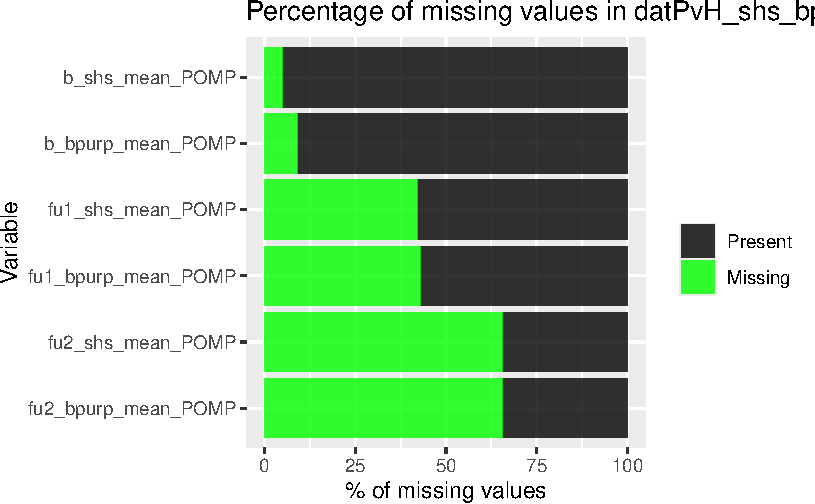
\includegraphics{purpose_vs_happiness_supplement_files/figure-pdf/missing_data-1.pdf}

\begin{Shaded}
\begin{Highlighting}[]
\CommentTok{\# create a missing data report}
\CommentTok{\#ZZZZ}
\end{Highlighting}
\end{Shaded}

\phantomsection\label{refs}
\begin{CSLReferences}{1}{0}
\bibitem[\citeproctext]{ref-steger2007}
Steger, Michael F., and Todd B. Kashdan. 2007. {``Stability and
Specificity of Meaning in Life and Life Satisfaction over One Year.''}
\emph{Journal of Happiness Studies} 8 (2): 161--79.
\url{https://doi.org/10.1007/s10902-006-9011-8}.

\end{CSLReferences}



\end{document}
